\documentclass[12pt,twoside]{book}
\usepackage[utf8]{inputenc}

% Style, symbols and language
\usepackage{libertine}
\usepackage[normalem]{ulem}
\usepackage{dsfont}
\usepackage{amsfonts}
\usepackage{amsmath}
\usepackage{amssymb}
\usepackage{amsthm}
\usepackage{mathtools}
\usepackage{cancel}
\usepackage{bm}
\usepackage[spanish,english]{babel}
%\usepackage[ruled, noline]{algorithm2e}
\usepackage[linesnumbered,ruled,vlined]{algorithm2e}
\SetKwInput{kwInit}{Init}


% Graphics, figures and colors
\usepackage{graphicx}
\usepackage{caption}
\usepackage{subcaption}
\usepackage{floatrow}
\usepackage{csquotes}
\usepackage[dvipsnames]{xcolor}
\definecolor{myColor}{HTML}{9B3035}
\definecolor{GIQOrange}{HTML}{C74B2A}

\usepackage{apptools}
\usepackage{titlesec}
\titleformat
{\chapter} % command
[display] % shape
{\bfseries\Huge} % format
{\filleft\,\scalebox{4}{\color{lightgray}\thechapter}} % label
{0.5ex} % sep
{   \rule{\textwidth}{1pt}
    \vspace{0.5 ex}
} % before-code
[
\vspace{-0.5 ex}%
\rule{\textwidth}{1pt}
] % after-code

% \usepackage{biblatex}%bibstyle=abbrv],backend=biber
\usepackage[backend=bibtex,citestyle=alphabetic,bibstyle=alphabetic,minalphanames=3,sorting=none,url=false]{biblatex}
%bibstyle= \usepackage[bibstyle=phys,citestyle=alphabetic,minalphanames=3,sorting=ynt,backend=biber]{biblatex}


\addbibresource{bibliography/1cv.bib}
\addbibresource{bibliography/1rl.bib}
\addbibresource{bibliography/intro.bib}
\addbibresource{bibliography/itw.bib}
\addbibresource{bibliography/disc.bib}

\addbibresource{bibliography/rlcoh.bib}
\addbibresource{bibliography/VANS.bib}
\addbibresource{bibliography/quantum.bib}
\addbibresource{bibliography/quantera.bib}
\addbibresource{bibliography/statinf.bib}
\addbibresource{publications.bib}


\usepackage[hidelinks]{hyperref}
\hypersetup{
     colorlinks = true,
     citecolor = magenta,
     linkcolor = magenta,
     urlcolor = magenta}


% Layout
\usepackage[a4paper,width=140mm,top=50mm,bottom=50mm,bindingoffset=6mm]{geometry}
\usepackage{fancyhdr}
\usepackage{afterpage}
\usepackage{hyperref}
\pagestyle{fancy} % \pagestyle{plain} changes to standard
\fancyhead{}
\fancyhead[LO]{\leftmark}
\fancyhead[RE]{\rightmark}
\fancyfoot{}
\fancyfoot[RO,LE]{\thepage}


\usepackage{tcolorbox}
% Miscellaneous
\usepackage{enumerate}
\usepackage[final]{microtype}
\usepackage{epigraph}
\usepackage{lipsum}
\usepackage{0hacks/shorthesis}

\renewcommand{\epigraphrule}{0pt}
\renewcommand{\epigraphflush}{flushleft}
\renewcommand{\textflush}{flushepinormal}
\renewenvironment{flushepinormal}{}{\vspace*{-1\baselineskip}}
\setlength{\epigraphwidth}{0.55\textwidth}
\usepackage[
    type={CC},
    modifier={by-nc-sa},
    version={3.0},
    imagemodifier={-eu-88x31}
]{doclicense}

\newcommand{\myTitle}{Decision-making in quantum environments:}
\newcommand{\mySubtitle}{from model-free to
model-aware learning of quantum controls}

\newcommand{\myName}{Matias Bilkis}
\newcommand{\myProfessor}{John Calsamiglia Costa}
\newcommand{\mySupervisor}{}
\newcommand{\myUniversity}{Universitat Autònoma de Barcelona}
\newcommand{\myFaculty}{Facultat de Ciències}
\newcommand{\myGroup}{Física Teòrica: Informació i Fenòmens Quàntics}
\newcommand{\myDepartment}{Departament de Física}
\newcommand{\myLocation}{Bellaterra}
\newcommand{\myTime}{Defense date\\ $12^{\text{th}}$ June, 2023}

\newcommand{\dbar}{d\hspace*{-0.08em}\bar{}\hspace*{0.1em}}

% Change line width of the fancy package
\renewcommand{\headrulewidth}{0.4pt}
\renewcommand{\footrulewidth}{0.4pt}

% \fancypagestyle{plain}{
%     \fancyhead[RO,LE]{\thepage} % Right Odd, Left Even => Outside
% }

\begin{document}
\frontmatter
%
\pagestyle{empty}
\begin{center}
\,
\vfill
    {\Large \color{myColor}{\textbf{\myTitle}}}
    \vspace{0.5cm}\\
    {\large \color{myColor}{\mySubtitle}}\\
    \vspace{0.5cm}
    by\\
    \textsc{\myName}
\vfill
\,
\end{center}

\pagestyle{empty}
\begin{flushright}
\,
\vfill
\textit{This page is intentionally left blank}
\end{flushright}

% -------------------------------------------------- %
% This is the title page of the thesis
% -------------------------------------------------- %

\begin{titlepage}
\begin{center}
    \vspace*{1cm}
    \myUniversity\\
    \vspace{1cm}
    {\Large \color{myColor}{\textbf{\myTitle}}}

    \vspace{0.25cm}

    {\large \color{myColor}{\mySubtitle}}

    \vspace{.5cm}
    by\\
    \textsc{\myName}
	\vspace{1 cm}

	under the supervision of \vspace{0.25cm}\\

	Prof. \textsc{\myProfessor,} \\

	\vspace{1 cm}

	A thesis submitted in partial fulfillment for the degree of \\
	Doctor of Philosophy in Physics
	\vspace{0.5cm}

    \myGroup \\
    \myDepartment, \myFaculty\\
    	\vspace{0.5cm}
    \includegraphics[width=4cm]{Figures/logos/giqlogo2.png}\\
    	\vspace{0.5cm}
	\myLocation, \myTime
\end{center}
\end{titlepage}

\pagestyle{empty}
\,
\vfill
\begin{flushright}
%\myName : \textit{\myTitle},\\
%\mySubtitle, \myTime.\\
\doclicenseThis
\end{flushright}

\pagestyle{empty}
\,
\vfill
\begin{flushright}
\textit{To my family and friends, \\ from here, there and beyond, \\ who supported me \\ during this amazing adventure.}
\end{flushright}
\vfill
\,

\pagestyle{empty}
\begin{flushright}
\,
\vfill
\textit{This page is intentionally left blank}
\end{flushright}

\chapter*{Abstract}
The success in the experimental control of quantum systems, along with the advent of artificial intelligence, raises the question of where do these worlds meet. In this thesis, a series of frameworks is proposed, in which a machine-learning agent sequentially interacts with a quantum system in order to learn control strategies. Such frameworks are interconnected with each other by the degree of knowledge the agent possesses on the setting at hand.

Our journey begins by model-free learning of long-distance quantum communication protocols, continues towards an intermediate-stage of awareness in which NISQ-computing problems are tackled, and finally lands on the fully-aware terrain, where statistical-inference problems are considered for continuously-monitored systems.

Specifically, we depart from a completely agnostic assumption, where a reinforcement learning agent is posed to the task of calibrating a quantum receiver that decodes information out of a continuous-variable system. From here, some light is shed into the learning problem, and in the second framework we consider how to design useful quantum circuits for currently-available quantum computers. To this end, a semi-agnostic algorithm that jointly optimizes both the structure and the parameters of the circuit is introduced. Finally, we consider how open quantum dynamics can be inferred by an agent which is continuously-monitoring a system. Here, the structure of the quantum evolution is assumed to be known, and the agent needs to learn which is the underlying hypothesis that describes systems’ dynamics out of a noisy measurement signal.

The methods developed in this thesis can potentially be applied to real-life scenarios, and represent a step forward towards the constitution of quantum machine learning.

\chapter*{Resum}
L’èxit en el control experimental dels sistemes quàntics, juntament amb la presència quotidiana de diferents intel·ligències artificials, planteja la pregunta d’on es creuen aquests mons. En aquesta tesi es proposa una sèrie de marcs en què un agent d’aprenentatge automàtic interactua seqüencialment amb un sistema quàntic per tal d’aprendre estratègies de control. Aquests marcs estan interconnectats entre si pel grau de coneixement l’agent té sobre l’escenari en qüestió.

El nostre viatge comença amb l’aprenentatge sense model de protocols de comunicació quàntica sobre llarga distància, continua cap a una etapa intermèdia de consciència en què s’aborden problemes de computació quàntica tipus NISQ i finalment aterra al terreny totalment conscient, on es consideren problemes d’inferència estadística en sistemes quàntics contínuament monitoritzats.

Específicament, partim d’un escenari completament agnòstic on un agent d’aprenentatge per reforç s’enfronta a la tasca de calibrar un receptor quàntic que descodifica informació clàssica d’un sistema quàntic de variable contínua. Partint d’aquest context, llancem una mica de llum sobre el problema de l’aprenentatge, i el segon escenari consisteix a dissenyar circuits quàntics útils per als ordinadors quàntics actualment disponibles. Per això, introduïm un algorisme semi-agnòstic que optimitza de manera conjunta tant l’estructura com els paràmetres del circuit. Finalment, considerem com la dinàmica d’un sistema quàntic pot ser inferida per un agent que està monitoritzant contínuament aquest sistema. Aquí, assumim que l’estructura de la dinàmica és coneguda per l’agent, que necessita aprendre quina és la hipòtesi subjacent que descriu l’evolució a partir d’un senyal de mesura sorollós.

Els mètodes desenvolupats en aquesta tesi estan preparats per poder ser aplicats a escenaris de la vida real i representen un pas endavant cap a la constitució de l’aprenentatge automàtic quàntic.
\setcounter{page}{1}

\chapter*{Resumen}
El control experimental exitoso de ciertos sistemas cuánticos, junto con la presencia de la inteligencia artificial, plantea la pregunta de dónde estos mundos se encuentran. En esta tesis proponemos una serie de marcos donde agente de aprendizaje automático interactúa secuencialmente con un sistema cuántico para aprender estrategias de control. Los marcos están interconectados entre sí por el grado de conocimiento el agente posee sobre el escenario en cuestión.

Nuestro viaje comienza con el aprendizaje sin modelo para protocolos de comunicación cuántica, continúa hacia una etapa intermedia de conciencia donde se abordan problemas de computación cuántica, y finalmente aterriza en el terreno totalmente consciente, considerando problemas de inferencia estadística en sistemas continuamente monitoreados.

En particular, partimos de una escenario agnóstico, donde un agente de aprendizaje por refuerzo se enfrenta a la tarea de calibrar un receptor cuántico que decodifica estados coherentes. Continuamos arrojando algo de luz sobre el grado de conciencia, y nuestro segundo escenario consiste en el diseño de circuitos cuánticos útiles para dispositivos actualmente disponibles. Para ello, introducimos un algoritmo semi-agnóstico que optimiza conjuntamente la estructura y los parámetros del circuito. Finalmente, estudiamos cómo inferir la dinámica de un sistema a partir de su monitoreando continuo. Aquí, asumimos que la estructura de la dinámica es conocida por el agente, quien necesita aprender cuál es la hipótesis subyacente que describe la evolución, a partir de la señal de medidas ruidosas.

Los métodos desarrollados en esta tesis están listos para ser aplicados a escenarios de la vida real y representan un paso adelante hacia la constitución del aprendizaje automático cuántico.

\pagestyle{empty}
\begin{flushright}
\,
\vfill
\textit{This page is intentionally left blank}
\end{flushright}

\chapter*{Declaration}
I declare that the thesis has been composed by myself and that the work has not been
submitted for any other degree or professional qualification. I confirm that the work
submitted is my own, except where work which has formed part of jointly-authored
publications has been included. My contribution and those of the other authors to this
work have been explicitly indicated below. I confirm that appropriate credit has been
given within this thesis where reference has been made to the work of others.
%I do also declare that Spanish crown means nothing to me.

\chapter*{Related works}
\begin{refsection}
    \small
    \nocite{bilkis2020realtime,bilkis2021semi,bilkisitw,gasbarri2023sequential,bilkis2023machine}
    \printbibliography[heading=none]
\end{refsection}
\noindent
\pagestyle{empty}
\begin{flushright}
\,
\vfill
\textit{This page is intentionally left blank}
\end{flushright}

\chapter*{Acknowledgments $\&$ Cariños}
\epigraphhead[10  ]{\epigraph{\textit{Gracias a la vida que me ha dado tanto }}{}}
Over all of the people I want to thank, John Calsamiglia (my PhD advisor) has undoubtedly been \textit{the} superhero. Among all the stuff he taught me ---which is certainly a lot by judging from the content of this thesis and our scientific collaborations---, there is one I want to highlight. Many issues, both scientific and life-related, have arisen during these years\footnote{As they say, \textit{La vida sin problemas es matar el tiempo a lo bobo.}}, and it was John who has taught me how to deal with such situations, and to find solutions without becoming desperate. These really subtle life lessons will mark me forever. I have no other words to thank this rather than saying that not only my scientific career but also personal life will be marked by this legacy. Per tot això, i tots aquests anys compartits, moltíssimes gràcies John!

Furthermore, this thesis would be really different if it wasn't for the two extraordinary post-docs I have worked with: Matteo Rosatti and Giulio Gasbarri. I also have no other words than big thanks to both of you, not only for the physics you taught me but also for the moments we enjoyed toghether.

During these years, the research group has been some sort of family to me, and it has been a pleasure to share the office with Matt, María, Minglai, Mani, Andreas, Anna, Ramón, Emili, Philipp, Gael, Suzana, Joe, Carlo, Naga, Illaria, Marco, Jennifer, Nikklas, Walther, Micha, Yago, Alonso, Jessica, Andreu, Antoni, Elisabeth, Esteban, Farzin, Zahra, and so many more!.

Tracing back a bit, I thank to all the people who encouraged me to move so far away from home to do this PhD. Above all, my family, who was an essential support during these times, even from so far away: mis viejos, mi hermana, Elena, Mariano, Flavia, Mandi, Paloma, mis abuelos Yaco, Scheine, Fanny y Abraham, Ruth, Tomi, Gonza, y todo el resto.

It was José Edelstein who first suggested me to move here (Barcelona); the Toni Acín, who has always been super receptive, was my first contact with this amazing city and got me in touch with GIQ. So big thanks to them!

Also, big thanks to all of my former teachers and collaborators from whom I have learnt and still learn so much; among them Mauricio Matera, Raúl Rossignoli, Norma Canosa, Lorena Rebón, Tomás Crosta, José Esté, Raul Morral, Marco Cerezo, Lukasz Cincio, Patrick Coles and Guillaume Verdon. Big thanks to the research institutions Instituto de Física La Plata and Los Alamos National Laboratory for hosting me during this years.

I also want to thank the unique support from people at Port d'Informació Científica (PIC), who lent me their computational resources which were essential to get most of the numerical results later analyzed in the thesis.

Also, I had an enormous help from my psychologist, who was essential to help me to take so many difficult decisions. Por el infinito apoyo durante estos años, muchas gracias Maren!

Son muchos años y por lo tanto mucha gente a la que agradecer, sin la cual toda esta aventura tampoco hubiera sido posible. Son al menos dos los lados del océano que toca agradecer, y las fronteras se suelen confundir épocas de tanta conexión. Sin más orden que el desorden, millones de gracias por todo el aguante a Valen Caso Rosendi, Caro Durián, Joaco Gil, Pedro Pablo, Javi Argüello, Mecchi Do Campo, Eric Kobrinsky, Amy Vianne, Sara Silva, Jero Penini, Seba Cabuli, Jose Giugno, Andi Sanelli, Ines Valla, Lucas Hadad, Nico Mártite, Nachito Piaggio (y toda la banda de natación platense!). Al maravishoso equipo Mashonesero: Cris Ceijas y Bea Astorga, a los vecinos de La Floresta y Vallvidrera: Carol Stankevicius, Ale Graziati, Taba Rios, Nati de la Fuente, Iña Allende, Lucho Griso y compañía. También Teresa Reinhard, Marta Solé Al Max Nordau en La Plata que siempre estará en mis raíces, a Lauti Krol, Pau Fioramonti, Eli Butinof, Juli Coloma, Joha Pronsky, Gasti Sal Anglada, Caro Bikis que es mi hermana pero ya que estamos la nombro de nuevo. ¡Cuánto aguante! También a Raulo Orcanza Rojas, Manu Hadad, Juli, Caro y Alicia Golijov (y Custom!). También Benja Ciancio, los Martines (Lagares y Tomé), Nahuel Díaz, Poe Enciso Porro, Pablo Gomez, Juani Sisti, Brian Evans, Floppy Espain, Sofi Lawrie, Manchi Machao, Nela Clinaz, Nacho Bruvera, Fiorela Ghilini, Cecchi, Lola Dafau-Saphores, Zenaida Andreica, Marta Fullola, A todo el equipo de triatló de la la Unió Ciclista de Sant Cugat! Cada persona que nombro me ha dado---y también las muchas que olvido nombrar---, durante estos años, un apoyo inigualable. Ah! and to my dog Dam that was always there (even virtually) for the routinary hugs :)

\pagestyle{empty}
\begin{flushright}
\,
\vfill
\textit{This page is intentionally left blank}
\end{flushright}

\include{Editorial/contents}

\mainmatter
\chapter{Motivation}
\epigraphhead[10  ]{\epigraph{\textit{It is imperfection - not perfection - that is the end result of the program written into that formidably complex engine that is the human brain, and of the influences exerted upon us by the environment and whoever takes care of us during the long years of our physical, psychological and intellectual development.}}{Rita Levi-Montalcini}}
Motivating this thesis should be quite easy, a friend told me a couple of days ago: just ask ChatGPT. However, I will not do this, and the main reason for that is because I have actually found joy during the writing of my thesis, and I think this is a good starting point. If we find pleasure in doing certain things, like research for example, why would we care in finding protocols to \textit{automatize} them, as done in this thesis? \textit{Ups}: tricky question.

Well, I can think of two reasons. The first one is for the fun in doing so: it has been (and still is) an amazing experience! Yes, definitely fun... but... it does not sound very convincing that my only motivation to do a PhD in quantum machine learning was only for the fun of it, right? %Also, let us just say it: this answer is a bit cliché, \textit{no?}

Thus, we need to think on a second reason. Think, think... come on... four and a half years thinking on this PhD and now nothing... Well, at least we can try to imagine the \textit{shape} of the answer. It should be something like... mmmm.... a bit harder to swallow... but not too much, since we really want to keep the reader up to (at least) the end of this Section. Exactly! that's the concept I need: ``Sections!''

While Sections help us structure things (and I can assure you, my Dear Reader that we \textit{will use them} later in the thesis), they do also place a distance between things. For us scientits, such distance is necessary --- and often essential --- in order to focus on an specific research topic. But more often than not, scientific communities (and we can well generalize this to the \textit{human knowledge}) fall into an abuse of \textit{knowledge compartmentalization}. And this sounds like a more satisfying motivation for why doing this PhD: work on connecting Science back. In turn, this thesis brings two fields that ---back to 2018, when my PhD began--- were quite far away from each other. Moreover, and as it happens in many situations when bringing two different worlds toghether, many beautiful things come up. While I will not play the card that quantum AI could lead to a major breakthrough ---I could sell it, but I don't buy it---  I do think that research directions that focus on intersecting different communities with each other are \textit{healthy} for science, and this is some kind of \textit{enough motivation} to me.

So what about \textit{quantum}? and what about \textit{AI}? Falling (perhaphs not too much!) in contradiction with the previous paragraph, let's go by parts.

Quantum theory is a route to understand physical reality, and I want to put emphasis on its fundamental aspects. Those have to do with describing reality by means of quantum superpositions and quantum correlations. Moreover, the theory is intrinsically stochastic in nature. Yet the physical reality that we inhabit has --- a priori --- nothing to do with this wierd phenomena of superpositions and non-local correlations. Furthermore, classical physics is intrinsically deterministic, in the sense that with precise knowledge of a given system, we can perfectly predict its behaviour. Some authors describe this gap as a desert of ignorance occupying many decimals in the scale. Then, how is our classical $\&$ deterministic perseption of reality reconciled with quantum theory? We simply do not know the answer yet, and this is perhaps one of the biggest misteries that we currently need to deal with.

On the other hand we have artificial intelligence (AI), and a huge (classical) computing power available ---at least to some--- right now. While ChatGPT and all the advent of AI is truly impressive, we are certainly not living in an Asimov's tale, and many questions remain open on how can current AIs become \textit{truly intelligent} as we humans are (if there even exists a clear definition for such concept). As of now, the possibility of an AI having the scientific \textit{aha!}s that we scientists are often illuminated with (call it \textit{intuition}) sounds like a fantasy. Perhaphs this will never happen, and our human condition hindered us to completely understand the logic behind our reasoning (be it concious or unconcious).

However, a PhD thesis consists in leaving almost all of the unresolved misteries of science, technology and humanity aside for a while, but focusing on only \textit{some}. And I guess this is what motivates the current thesis: on the one hand there is clear evidence that we can control quantum systems up to an unprecedented level\footnote{By this, we mean preparing and storing a system in a quantum superposition for a sufficiently long time.}. On the other hand, while current AIs might be a game-changer in a volatile society like ours, they do not represent a change-of-paradigm on how intelligence is understood, as they do not even get close to it. This might sound polemic, I know, since for example ChatGPT has recently passed Scott Aaranson's quantum-mechics exam with a 7/10 score. However, I do refer to intelligence as something beyond passing an exam. Again, I would be truly impressed (and of course chances are that I am wrong) that an AI had an \textit{aha!} all of a sudden, and came up with a new theory of knowledge on its own, \textit{i.e.} without human intervention. AI should be understood as a tool, and not as a stand-alone system.

\bigskip
In this thesis, we pay special attention to the currently available quantum technologies, by considering three paradigmatic devices. First we will study continuous-variable quantum receivers, which are aimed to decode information out of a quantum state of light. Secondly, we focus on NISQ computers, which are relatively small and extremely noisy version of quantum computers, but have already been able to provide a quantum advantage with respect to any classical computer paradigm (though for a very specific task). Thirdly, we will consider the case of continuous-time quantum sensors, where a quantum system stored in an optical cavity is being monitored, which provides an effective way to infer information about its environment.

In this thesis we tackle each of the aforementioned devices ---also called quantum environments--- from the machine-learning perspective. This is done by introducing an agent equipped with a varying level of awareness on the quantum environment that is faced to.

The phyisical systems that we consider, along with the methods and machine-learning algorithms, are
widely explained in the \textit{Preliminaries} Chapter. This (considerably long) chapter serves as a reference for the subsequent ones. Thus, the reader can straightfowardly begin from any Chapter, and consult the \textit{Preliminaries} when necessary (appropiate reference are included).

The learning journey begins \textit{in the darnkness}, where the agent is asked to optimally callibrate a quantum receiver without any knowledge of the setting at hand. Here, the only information given to the agent is a binary reward (a bit, valued either 0 or 1), which stands for the correctness of the guess made for the underlying signal that is aimed to be decoded.

We continue \textit{in the twilight}, with an agent facing the problem of building noisy quantum circuits, in the context of NISQ computing. Here, the solutions the agent is asked to reach are even unknown to us, and we can only aid her by providing specifically-tailored circuit compression rules. To this end, we introduce the VAns algorithm, which sequentially modifies the quantum circuit by following a variable-ansatz structure. Our method is thoroughly tested in paradigmatic quantum machine learning applications, ranging from VQE to quantum autoencoder tasks.

Finally, we \textit{learn during daylight}, where a fully model-aware agent is asked to tackle statistical inference problems. Here, our attention is put on continuously-monitored quantum systems, where the performance of sequential discrimination protocols is studied. Here, we analytically study the evolution of the log-likelihood ratio, by providing insight on error rates and stopping time probability distribution for a sequential test. In addition, the case of parameter estimation is considered, and a maximum-likelihood estimation is carried out by an automatic-differentiation method; such recurrent structure allows us to infer parameters of external signals out of the measurement signal.

The main contribution of this thesis is that of `` bringing the quantum scientist closer to the AIs, in such a way that they can collaborate with each other". This thesis, as most of the scientific research, provides a (small) step further towards the constitution of such collaboration. Having this in mind, the reader shall not understand each of the Chapters as a closed-one, but rather as an invitation to continue writing it. In turn, our results do not constitute a milestone in quantum AI, but we rather see them as blueprints towards more ellaborate quantum AI framework.

\pagestyle{fancy}

\chapter{Preliminaries}
\epigraphhead[12  ]{\epigraph{\textit{Yo no se qué pasó // en mil calles la calle se abrió. // Me perdí y en verdad // no sabía que rumbo tomar//. Pregunté, porque al fin // preguntando se llega a Pekín. }}{--- Lo que me costó el Amor de Laura \\ Alejandro Dolina}}
This chapter is aimed to explain both physics and algorithms studied in the thesis.

We begin with quantum physics; after recaping the basic ingredients of quantum information in Sec.~\ref{sec:1_introquantum}, we discuss about (discrete-variable) NISQ computing in Sec.~\ref{sec:1_nisq}. We then review continuous-variable quantum systems in Sec.~\ref{sec:1_cv}, with a particular focus on Gaussian states and operations. Introducing such a formalism allows us to discuss continuously-monitored systems in Sec.~\ref{sec:1_cmon}, and this consitutues the end of our tour through quantum systems.

Thus, in Sec.~\ref{sec:1_statinf} we turn to the classical world by discussing statistical inference problems, we discuss hypothesis-testing in Sec.~\ref{ssec:1_hypo_testing}, and consequently introduce the quantum state discrimination problem in Sec.~\ref{ssec:1_qdisc}. Moreover, we discuss parameter estimation in Sec.~\ref{ssec:1_stinf_estimation}.

Finally, we introduce the reinforcement learning framework in Sec.~\ref{sec:1_rl}, with a particular focus on model-free Q-learning agents.

\section{Some basic notions of quantum information}

A system $\mathcal{S}$ is described by quantum theory using a $d$-dimensional Hilbert space $\mathcal{H}$; the dimension $d$ might be infinite, \textit{e.g.} if we want to describe systems in the continuous-variable (CV) ones, such as optical or mechanical ones. The state of the system is represented by a self-adjoint, positive semi-definite and unit-trace operator $\rho\in\mathcal{H}$.

Physical quantities such as position, angular momenta or energy are described by self-adjoints operators, known as observables. As such they have an associated eigenbasis, each eigenstate being a unit-vector in $\mathcal{H}$ and deemed \textit{pure state}. Note however that a quantum state is generally found in a \textit{mixed state}, \textit{e.g.} a probabilistic mixture of pure states.

The value that physical quantities can take is obtained by measuring the system, and this makes quantum theory a \textit{physical} one, since we can readily contrast measurement statistics with theoretical predictions.

Given an orthonormal basis $\llaves{\ket{i}}_{i=1}^d$, a quantum state\footnote{While much of the following discussion applies to CV systems as well, we will restrict in this Section to finite $d$, and study CV-systems in Sec.~\ref{sec:1_cv}.} can be written as
\equ{\rho = \sum_{i,j}\rho_{ij}\ketbra{i}{j},} where $\rho_{ij}$ are the matrix components of $\rho$. Since $\rho\>0$, its spectral decomposition is always available, with an associated  eigenbasis $\llaves{\ket{k}}$
\equ{\rho = \sum_k p_k \proj{k},\spacee 0 \leq p_k\leq, \spacee \sum_k p_k=1,} where the conditions on $p_k$ arise from the fact that $\rho$ is positive semi-definite and unit-trace operator. The purity of the state is defined as $\tr{\rho^2}$; while pure-states are represented by rank-one operators (of purity $1$), mixed-states' purity is strictly less than $1$.

Composite systems are described in a Hilbert space formed by the tensor-product of the individual components. As an example, let us consider bipartite systems with parties $\cS$ and $\cA$; the composite quantum state $\rho_{SA}$ is an operator in $\mathcal{H}_{\cS \cA} = \mathcal{H}_\mathcal{S}\otimes \mathcal{H}_\mathcal{A}$. Taking a basis for $\mathcal{H}_{\cS \cA}$ formed by a tensor-product of basis $\ket{i_S}$ and $\ket{j_A}$ in $\mathcal{S}$ and $\mathcal{A}$ respectively, we obtain that
\equ{\rho_{AS} = \sum_{ijkl}\rho_{ij}^{kl} \ketbram{i}{S}{j}\otimes\ketbram{k}{A}{l}.} A state is \textit{separable} if it can be written as a convex combination of product-like states, \textit{i.e.}
\equ{\rho_{AS}^{sep} = \sum_k p_k \rho_S^{(k)} \otimes \rho_A^{(k)},} where $\rho_i^{(k)}$ is a \textit{local} quantum state in subsystem $i=S,A$. If $\rho_{AS}$ cannot be written in this form, then the state exhibits quantum correlations.

The reduced state of each subsystem is defined via the partial-trace~\cite{nielsen00}; \textit{e.g.} $\rho_{S(A)} = \text{Tr}_{A(S)}\left[\rho_{AS}\right]$. For instance, the local state of system $\mathcal{S}$ reads
\equ{\rho_S = \tr{\rho_{AS}} = \sum_m \bra{m_A}\Big(\sum_{ijkl} \rho_{ij}^{kl} \ketbram{i}{S}{j} \otimes \ketbram{k}{A}{l}\Big)\ket{m_A} = \sum_{ijm} \rho_{ij}^{mm} \ketbram{i}{S}{j}.}

\subsubsection{Projective measurements}

In order to extract information out of a quantum state, we need to measure it. Quantum measurements deliver a classical outcome, and provide a route to map quantum information to classical one. While generalized measurements will be discussed in Sec.~\ref{ssec:1_intro_qmeas}, we will now discuss a particular type of measurement.

Projective measurements consist on orthogonal projectors $\llaves{E_k}$ such that $E_k E_j = \delta_{kj}E_j$, with $\sum_k E_k = \mathbb{I_d}$, and $E_k = E_k^\dagger$. Here, the possible measurement outcomes are $\llaves{k}_{k=0}^{d-1}$, and the probability of outocome $k$ given the state of the system is $\rho$ reads\equ{p(k) = \tr{\rho E_k}.} Moreover, the state of the system after this outcome occurs, known as the post-measurement state, is given by \equ{\rho \rightarrow \rho_{|k} = \frac{E_k \rho E_k}{\tr{\rho E_k}},} where we note that the normalization is given by the probability of such measurement outcome. On the contrary, if the measurement is performed bu the outcome is not known, the \textit{unconditional post-measurement state} is given by \equ{\rho \rightarrow \sum_k E_k \rho E_k.}Here, we observe that \textit{(i)} the unconditional state is the average of all possible conditional-states, as weighted by the corresponding probability $p(k)$, and \textit{(ii)} if the original state to be measured is pure, then not recording the measurement outcome will generally convert it to a mixed state.

As an example, let us consider an observable $O$. We can readily construct a projective measurement via its spectral decomposition, \textit{i.e.} $\hat{O} = \sum_k o_k \proj{k}$, leading to $E_k = \proj{k}$ and
\equ{\expect{O}_\rho = \tr{\hat{O}\rho} = \sum_k p_k o_k,}
where $p_k = \tr{\rho \proj{k}}$ is the probability of finding the state $\rho$ in the $k^{th}$ eigenstate of $\hat{O}$. Here, let us recall that if $\hat{H}$ is the system's Hamiltonian, then \textit{the variational theorem} is obtained by noting that $p_k\geq0 \;\forall k$; it follows that $\expect{H}_\rho\geq E_0$ where $E_0$ is the ground-state energy, \textit{i.e.} the lowest eigenvalue of $\hat{H}$. The inequality is saturated in the case that $\rho$
is the ground-state of $\hat{H}$; this is the basis of variational quantum algorithms, where $\rho$ is evolved in such a way to get as close as possible to the ground-state, as discussed Sec.~\ref{sec:1_nisq}.

\subsection{Closed-system dynamics}\label{ssec:1_intro_unitary_evo}
The evolution of a closed quantum system is given by an unitary transformation $\hat{U}_t$, generated by a Hamiltonian $\hat{H}$, \textit{e.g.} $\hat{U}_t = e, {-\ii \hat{H}t}$, where the Hamiltonian will be assumed time-independent. Here, the Schrodinger equation describes quantum-state evolution according to
\equ{\partial_t \rho(t) = -\ii \comm{\hat{H}}{\rho(t)}.} The solution to such equation can be expressed as \eq{schro}{\rho(t) = \hat{U}_t\rho(0)\hat{U}_t^\dagger,} and this constitutes the \textit{Shcrodinger picture}.
However, the time-dependence of the quantum state can be entirely translated to the observables, which gives rise to the \textit{Heisenberg picture}. In turn, by defining \equ{\hat{O}(t) = \hat{U}^\dagger \hat{O}(0) \hat{U},}we observe that the expected value of $O$ reads \equ{\expect{O}(t) = \tr{O(0)\rho(t)} = \tr{O(t)\rho(0)}.} The correspoding equation of motion for the observable reads
\equ{\partial_t O(t) = \ii \comm{H}{O(t)}.}
Moreover, the \textit{interaction picture} ---or interaction frame--- is obtained by decomposing the Hamiltonian in terms of the \textit{free} Hamiltonian $H_0$ and an interaction term $V$ according to $H=H_0 + V$. In this picture, both states and observables depend on time, according to \equ{\rho_{IF}(t) = e^{-\ii H_0 t} \rho(0)e^{\ii H_0 t},}\equ{\hat{O}_{IF}(t) = e^{-\ii H_0 t}\hat{O}(0)e^{\ii H_0 t},} and the evolution of $\rho_{IF}(t)$ reads \equ{\partial_t \rho_{IF}(t) = -\ii \comm{V}{\rho_{IF}(t)},}
where a similar evolution applies for observables as well.
% Let us now turn to quantum measurements, which link the quantum to our (classical) world.

Changes in quantum-states can be generalized to consider the case in which the quantum system is interacting with an environment, \textit{i.e.} an open-quantum system. While our discussion of the continuous-time case will be postponed until Sec.~\ref{ssec:1_intro_open}, we will now introduce a tool to represent discrete changes, such as those modeling the noise that a quantum-receiver suffers, as studied in Sec.\ref{ssec:rlcoh_noise}, or the noise injected into a quantum state by an imperfect NISQ-component, as we study in Sec.~\ref{ssec:vans_results_noise}.

\subsection{Quantum channels}\label{ssec:1_intro_channels}
A quantum channel $\Phi$ is a lineal map $\Phi:L(\mathcal{H}_1) \rightarrow L(\mathcal{H}_2)$, where $L(\mathcal{H})$ denotes the set of operators in $\mathcal{H}$ and the dimensions of the input-space $\mathcal{H}_1$ and output-space $\mathcal{H}_2$ might differ.

The lineal map is required to be:
\begin{itemize}\item Completely positive (CP): let $\mathcal{H}_{1'}$ be of dimension $d'$, then \equ{(\mathbb{I}_{d'}\otimes\phi)[\sigma]\geq0\;\forall d', \;\forall \sigma \in \mathcal{H}_{1'}\otimes \mathcal{H}_1.}
\item Trace-preserving (TP).
\end{itemize}The first condition is required such that when $\Phi$ acts locally (\textit{i.e.} on one out of many subsystems), the resulting global state is a positive state. The second condition is required such that the resulting state is unit-traced.

Choi-Krauss theorem~\cite{manzano2019} guarantees that any CPTP channel admits a \textit{Kruss} decomposition:
\begin{equation}
\mathcal{M}(\rho) = \sum_{k=1}^N M_k \rho M_k^\dagger,
\end{equation}
with
\eq{compKraus}{\sum_{k=1}^N M_k^\dagger M_k = \mathbb{I}_d.}
The operators $\llaves{M_k}_{k=1}^N$ are known as \textit{Krauss operators}, and it is important to note that this decomposition is not unique.

The non-uniqueness of Krauss decomposition is explicited by the \textit{Stinespring dillation}. This states that any CTPT channel can be obtained by unitarily evolving the input-system with an ancilla and tracing the latter out. To see this, let the initial state of the system and ancilla be $\rho$ and $\proj{0_A}$ respectively, and the closed (unitary) evolution of the joint system given by $\hat{U} = \hat{U}_{SA}$. The resulting state of the system is
\begin{align}\label{eq:stinesrping}
\rho \rightarrow& \text{Tr}_A\left[\hat{U} \rho \otimes \proj{0_A} \hat{U}^\dagger\right] \\
=& \sum_{k=1}^N \langle k_A| \Big( \hat{U} \ket{0_A} \rho \bra{0_A} \hat{U}^\dagger \Big) \ket{k_A}\\
=& \sum_{k=1}^N M_k \rho M_k^\dagger,
\end{align}
where we defined $M_k = \langle k_A|\hat{U} \ket{0_A}$ by considering a basis $\llaves{\ket{k_A}}_{k=1}^N$ of the ancilla. However, we can readily note that a different basis $\llaves{\ket{\nu_A}}_{k=1}^{N'}$ (of a possibly enlarged) ancilla could be considered, where the basis-elements are related to each other by an isometry $\hat{V}$ such that $\ket{\nu} = \sum_{l=1}^{N} V_{\nu k}\ket{k}$. Using the latter basis, the two sets of Krauss operators relate to each other as $N_\nu = \sum_{l=1}^{N} V^\dagger_{\nu k} M_k$.

Morever, note that the map $\Phi$ will be trace-preserving iff $\sum_{k=1}^N M^\dagger_k M_k = \mathbb{I}$. Also, we remark that as long as Eq.~\ref{eq:compKraus} is satisfied, the Krauss operators can also be time-dependent~\cite{manzano2019}.

As an example, we can consider an unitary channel as in Eq.~\ref{eq:schro}, where the Krauss representation reduces to $M_k = \hat{U}_t$, with $N=1$.

\subsection{Generalized quantum measurements}\label{ssec:1_intro_qmeas}

A generalized quantum measurement given by a set of lineal operators $\llaves{E_k}_{k=1}^n$, each associated to a possible outcome $k \in \llaves{1,...,n}$. The probablity that outcome $k$ happens, conditioned on the quantum state being $\rho$, is given by the Born rule: \eq{bornrule}{p(k|\rho) = \tr{\rho E_k}.} Since such probability is required to be positive for any quantum state, it follows that $E_k\geq0$ (which imply self-adjointness). Moreover, since $\sum_k p(k|\rho) = 1$ for any quantum state, then $\sum_k E_k = \id_d$. This constitute a \textit{Positive Operator-Valued Measure (POVM)}, which we will often denote by $\mathcal{M}$.

POVMs arise when a projective measurement is carried out on an ancilla that the system is coupled with. Similarly to our previous discussion on quantum channels\footnote{In fact, measurements can be regarded as quantum-to-classical channels~\cite{watrous_2018}}, we can readily define an ancilla system $A$, with an associated eigen-basis $\llaves{\ket{k_A}}_{k=1}^n$. Now, considering the initial-state of the system and ancilla to be $\rho_S$ and $\proj{0_A}$ respectively, and the joint unitary evolution to be $\hat{U}$, a projective measurement $\llaves{\proj{k_A}}$ carried out on sub-system $A$ will occur with probability \equ{p(k) = \tr{(\id_d \otimes \proj{k_A}) \rho_s \otimes \proj{0_A}} = \tr{\rho M_k^\dagger M_k} = \tr{\rho E_k},}
where similarly to the previous Section we have $M_k=\langle k_A|\hat{U}\ket{0}$. Thus, under this Krauss decomposition we have that $E_k = M_k^\dagger M_k$, and the conditional state of $\rho$ upon obtaining measurement outcome $k$ reads
\equ{\rho \rightarrow \rho_{|k} = \frac{M_k \rho M_k^\dagger}{\tr{\rho M_k^\dagger M_k}}.}Similarly, the unconditional post-measurement state under such Krauss decomposition reads
\eq{measurementdynamics}{\rho \rightarrow \sum_k^n M_k \rho M^\dagger_k.}It is important to recall that this decomposition is not unique, since different Krauss decompositions are equivalent by an isometry, as discussed in the previous Section. In turn, Eq.~\ref{eq:measurementdynamics} can be understood as a quantum channel acting on $\rho$, similar to Eq.~\ref{eq:compKraus}. In this direction, it is useful to understand different Krauss decompositions as different \textit{unravelings} of the open-quantum system dynamics, all averaging up to the same unconditional evolution.

The notion of quantum measurements and channels can be generalize to take into account stochastic channels, using the concept of a quantum instrument~\cite{watrous_2018} ,or quantum operation~\cite{Preskill1998}, which we now turn to introduce.
\subsection{Quantum instruments}\label{ssec:1_intro_operations}
A quantum instrument is described by a collection of CP maps $\llaves{\phi_k}_{k=1}^n$, which sum up to a channel, \textit{i.e.} $\Phi = \sum_k \phi_k$. Such object is to be considered as a generalization of a POVM: after applying a quantum instrument on a state $\rho$, two things happen:\begin{itemize}\item A measurement outcome $k$ is obtained with probability $\tr{\phi_k(\rho) }$,\item The conditional state of $\rho$ upon observing measurement outcome $k$ is \equ{\rho \rightarrow \frac{\phi_k(\rho)}{\tr{\phi_k(\rho)}}.}\end{itemize}
We can readily consider a krauss decomposition of $\phi_k$, given by $\llaves{M_{k \mu}}$. Such Krauss operators should obey the completeness relation derived above, namely $\sum_{k \mu} M^\dagger_{k \mu} M_{k \mu} = \id$. Here, we can interpret the quantum instrument as an object describing an stochastic application of $\phi_k$: whereas $k$ is recorded, the label $\mu$ is ignored. As such, the post-measurement state reads\equ{\phi_k(\rho) = \sum_\mu M_{k\mu}\rho M_{k\mu}^\dagger,}with outcome $k$ occuring with probability $p(k) = \tr{\phi_k(\rho)}$. We note that since outcome $\mu$ is ignored, the channel $\phi_k$ is generally trace-decreasing, and the normalized post-measurement state coincides with the post-measurement state defined above as $\rho_{|k} = \frac{\phi_k(\rho)}{\tr{\phi_k(\rho)}}$.

Moreover, we might think of a process that consists on $M$ consecutive measurements, leading to an stochastic sequence $\bm{k} = \llaves{k_1, ..., k_j,... k_M}$. The conditional state of the system upon observing outcome $k_j$ is obtained via $\phi_{k_j}$. Note that when keeping the system's state unnormalized up to the $M$-outcome, the trace of the unnormalized state, \textit{i.e.} $\phi_{k_M} \circ....\circ \phi_{k_1} (\rho)$, represents the likelihood of observing such sequence of outcomes, and the normalized state reads:
\equ{\rho_{|\bm{k}} = \frac{\phi_M \circ....\circ \phi_1 (\rho)}{\tr{\phi_{k_M} \circ....\circ \phi_{k_1} (\rho)}}.}

Our discussion has so-far limited to discrete changes of the quantum state. In the following we will discuss how a dynamical equation is obtained for the (unconditional) evolution of an open-quantum system.
\subsection{Quantum master equation}\label{ssec:1_intro_open}

While we have previously introduced the notion of a quantum channel given by a CPTP map between quantum states, no notion of continuous-time has entered so-far in the discussion. Thus, we will here consider a quantum channel $\cE _t$, and discuss a dynamical equation accounting for $\rho(t)  = \cE _t[\rho(0)]$. In the Markov approximation, this can be expressed as a differential equation of the form
\equ{d\rho = \cL[\rho] dt,}
where $\cL$ is a superoperator that generates the \textit{quantum dynamical semi-group}
\footnote{A quantum dynamical semi-group consists on a family of CPTP maps $\llaves{{\cE}_t:t\geq0}$ such that \textit{(i)} $\cE _t \cE _s=\cE _{t+s}$ and \textit{(ii)} $\tr{\cE _t [\rho] \hat{O}}$ is continuous over $t$, for any state-observable pair $(\rho, \hat{O})$. Note that the first restriction is quite restrictive, since an aritrary evolution might not admit such decomposition.}
associated to $\cE _t$ and can be shown to admit the so-called \textit{Lindblad form}~\cite{libland1976, wisemanbook, manzano2019}:
\begin{equation}\label{eq:libland}
\cL(\rho)= -\ii\comm{\hat{H}}{\rho} +  \sum_{k=1}^{M} \cD[\hatL_k]\rho, \spacee \cD[\hatL_k]\rho = \hatL_k \rho + \rho \hatL_k^\dagger - \frac{1}{2}\llaves{\hatL_k \hatL_k^\dagger, \rho},
\end{equation}
where $\hat{H}$ is the system Hamiltonian (generator of the closed-system dynamics) and the linearly-independent operators $\llaves{L_k}$ are known as the \textit{Lindblad operators}, or \textit{jump operators}. We note that the Lindblad form is invariant under \textit{(i)} unitary transformations of the jump operators, \textit{i.e.} $\hatL_k \rightarrow \sum_l \hat{V}_{kl}\hatL_l$ with $\hat{V}$ unitary (which is a consequence of the unitary invariance of the Krauss decomposition), and
\textit{(ii)} shifts of the Lindblad operators accompanied by a new term in the Hamiltonian:
\begin{equation}\label{eq:invalibland}
\hatL_k \rightarrow \hatL_k + \xi_k, \spacee \hat{H} \rightarrow \hat{H} - \frac{\ii}{2}\sum_{i=1}^M \xi_k^* \hatL_k - \xi_k {{\hatL}^\dagger}_k.
\end{equation}
The dynamical equation introduced above is known as the \textit{quantum master equation}, and its generator is given by Eq.~\ref{eq:libland}. We remark that this evolution can also be obtained by suitable time-dependent Krauss operators:
\begin{align}\label{eq:ravel}
\rho(t+dt) = \cE_{dt}[\rho(t)] =& \rho + \sum_{k=1}^M K_k(dt) \rho K^\dagger _k(dt) \\
=& \rho + \cL[\rho] dt.
\end{align}
As discussed in Sec.~\ref{ssec:1_intro_qmeas}, the choice of Krauss and jump operators $K_k(dt)$ in Eq.~\ref{eq:ravel} plays an imporant role when studying the \textit{conditional} dynamics, arising as a consequence of recording the measurement outcome at each time-step. This can be understood as an stochastic sequence of channels, as introduced in Sec.~\ref{ssec:1_intro_operations}, which give rise to the notion of a \textit{quantum-trajectory}, as discussed in Sec.~\ref{sec:1_cmon}.

\vspace{2cm}
To conclude, in this Section we have revisted some of the basics in quantum information theory. Many of the concepts discussed here will be recaped later in the thesis. We will now turn to introduce some of the physics and concepts that set the basis for Chapter~\ref{chapter:VANS}.
\label{sec:1_introquantum}
\section{NISQ $\&$ the qubits}\label{sec:1_nisq}
In this Section we will focus on discrete-variable systems. Special attention will be payed to Noisy Intermediate-Scale Quantum (NISQ) computing, a concept standing for currently available technologies, where quantum circuits of about $50-100$ qubits are already being implemented and controlled despite the strong presence of noise~\cite{preskill2018quantum}.

While error-correcting codes cannot be built with such a low amount of qubits ---it is estimated that nearly a thousand \textit{physical qubits} are required in order to get a single \textit{logical qubit}~\cite{Fowler2012surface}--- special-purpose quantum devices can readily be built, exhibiting a genuinely quantum behaviour. Whether such techologies will be able to provide a game-changer quantum advantage in industry applications, or they are just a stepping stone towards fault-tolerant architectures is a matter of vivid debate between the community~\cite{supremacygoogle,nosupremacy,chemistrynono}. However, we remark that the sole feasibility of experimental preparation and control of quantum systems already constitute a game-changer paradigm in our scientific community. In turn, not only a plethora of new questions regarding scalability and overall implementation of such techologies arise~\cite{useful2discoverQC}, but also the demand for new theoretical tools, particularly to better analyze performance issues that we will later discuss~\cite{mcclean2018barren,cerezo2020cost,pesah2020absence,holmes2020barren,zhao2021analyzing,thanasilp2021subtleties,sharma2020trainability,patti2020entanglement,marrero2020entanglement,cerezo2020impact,arrasmith2020effect, npHardVQA}.

In the following we will concentrate on an specific topic that falls under the umbrella of NISQ computing, called Variational Quantum Algorithms.

\subsection{Variational Quantum algorithms}\label{ssec:1_nisq_vqa}
Recently, a superpisition of hype and hope has been put on the  %~\cite{preskill2018quantum, peruzzo2014variational, pesah2021absense,sharma2022reformulation,biamonte2017quantum
field of quantum machine learning~\cite{biamonte2017quantum, supremacygoogle, schuld2021isquantum, Aaronson2015, preskill2018quantum, peruzzo2014variational, pesah2021absense,sharma2022reformulation}, particularly when \textit{training} Parametrized Quantum Circuits (PQCs).

PQCs consists on a series of quantum gates, \textit{e.g.} CNOTs and rotations, where the real parameters of the latter are modified in order to \textit{optimize} the circuit. Here, and in analogy to the classical neural networks scenario~\cite{Goodfellow-et-al-2016}, we aim to minimize a given cost function (and thereby, these circuits are also known as \textit{quantum neural networks}). The overall training of PQCs is known as a Variational Quantum Algorithm (VQA), and consists on an hybdrid classical-quantum scheme. In turn, a quantum device is only used to estimate cost-function values, whereas a classical algortihm is in charge of controlling that quantum device by optimizing over accessible degrees of freedom, \textit{e.g.} rotation parameter values. Recently, many efforts have been carried out in order to analyze the performance, trainability and overall feasibility of VQAs~\cite{VQA_revmarco, VQA_revalba}.

Training a VQA means to solve an optimization problem encoded into a cost function of the form
\begin{equation}\label{eq:cost}
    C(\kvec,\thv)=\sum_i^M f_i\left(\tr{\Oi U(\kvec,\thv)\rho_i U^\dagger (\kvec,\thv)}\right)  \,.
\end{equation}
Here, $\{\rho_i\}$ are $n$-qubit states forming a \textit{training set} of cardinality $M$, and $U(\kvec,\thv)$ is our NISQ circuit parametrized by continuous parameters $\thv$ (\textit{e.g.}, rotation angles) and by discrete parameters $\kvec$ (\textit{e.g.}, gate placements). Moreover, $\Oi$ are observables and $f_i$ are functions that encode the optimization task at hand.

For example, when employing the Variational Quantum Eigensolver (VQE) algorithm~\cite{peruzzo2014variational} we have $f_i(x)=x$ and the cost function reduces to
\eq{vqe_cost}{C_{\text{VQE}}(\kvec,\thv)=\tr{\hat{H} U(\kvec,\thv)\rho U^\dagger (\kvec,\thv)},}where $\rho$ is the input state (and the only state in the training set) and $H$ is the Hamiltonian whose ground state we seek to prepare. Alternatively, in a classification problem where the training set is of the form $\{\rho_i,y_i\}$, with $y_i\in \{1,...,n\}$ being the true label, the choice $f_i(x)=(x-y_i)^2$ leads to the least square error cost~\cite{classiVQA, vqaclass1, vqaclass2,vqaclass4, cong2019quantum}.
In this regard, and as it happens in the reinforcement-learning scenario discussed in Sec.~\ref{sec:1_rl}, the possibility of encoding a given problem into a cost function is a matter of creativity.

\vspace{1cm}

Given the cost function, a NISQ circuit is employed to estimate each term in Eq.~\eqref{eq:cost}. Ussually, the available measurements consist on local projections over the eigenbasis of $\sigma^{i}_z$ for each qubit $i=1,...,n$. Here, in order to estimate the cost function, we decompose each operator appearing in the cost-function in terms of \textit{Pauli-strings}. Recall that Pauli-string operators form a basis in the space of $n$-dimensional hermitian operators and hence
\eq{decoH}{ \Oi = \sum_{k=1}^{4^n} c_k P_k,}
with $P_k = \bigotimes_{i=1}^n\mathbb{\sigma}_j$, where $\mathbb{\sigma}_j \in \llaves{\mathbb{I}, \sigma_x, \sigma_y, \sigma_z}$. Note that Pauli-string operators are orthogonal to each other, \textit{i.e.} $\tr{P_k P_{k'}} = 2^n \delta_{k k'}$ and thus $c_k = \tr{\Oi P_k}/2^n$.

Thus, the cost-function can be estimated by computing averages of some pre-determined observables, which are in turn a weighted sum of expected values of Pauli-strings. Moreover, we can estimate each expected value $\langle P_k\rangle$ by performing the corresponding single-qubit transformation beforehand and measuring $\sigma_z$\footnote{This can be understood as a change-of-basis.}. In this regard, if an $\epsilon$-accuracy is required in order to estimate this expected value, an order of $\sim \frac{1}{\epsilon^2}$ measurements needs to be done (this will have consequences when trying to resolve between very small values of the cost-function in Sec.~\ref{ssec:1_nisq_barrenplateaus}).

We also note that the Pauli-string procedure outlined above consists on an exponentially large sum of expected values. However, we are often interested in local hamiltonians, where many of these terms vanish (for example, TFIM and XXZ models considered in Ch.~\ref{chapter:VANS}). In this case, techniques such as randomized measurements (RMs) have recently been developed, in which the cost function can be computed more efficiently. While we do not consider such approaches in this thesis, we refer the interested reader to Ref.~\cite{elben2022randomized}, and we note that a combination between our methods (discussed in Chapter~\ref{chapter:VANS}) and classical shadows (a sub-class of RMs) is discussed in Sec.~\ref{ssec:vans_discu}.

\vspace{1cm}

Once the cost-function has been estimated, the power of classical optimization algorithms is leveraged to solve the optimization task
\begin{equation}\label{eq:optimization}
    \argmin{\kvec,\thv} C(\kvec,\thv)\,.
\end{equation}
\begin{figure}[t!]
    \centering
    \includegraphics[width=1.\textwidth]{Figures/VANS/vqa_cycle.png}
    \caption{Figure adapted from Ref.~\cite{borrowed}: a generic VQA algortihm is sketched. Here, a quantum device is used to estimate a cost-function value, whereas the device itself is controlled by a classical optimization algorithm. This cycle is iterated until convergence.}
    \label{fig:VQAcycle}
\end{figure}
The estimation of a cost function via a quantum circuit and its modification (hopefully towards a cost-minimizing direction) by a classical optimization algorithm defines a cycle, which is repeated until convergence, as depicted in Fig.~\ref{fig:VQAcycle}. The success of such scheme hinges on several factors. As a matter of fact, the classical optimizer must be able to efficiently train the parameters, and in the past few years, there has been a tremendous effort in developing quantum-aware optimizers~\cite{verdon2018universal,kubler2020adaptive,arrasmith2020operator,stokes2020quantum,koczor2019quantum,nakanishi2020sequential,fontana2020optimizing}. In particular, severe trainability issues has been pointed out, which forbid the success of VQAs and as constitute the main barrer (along with hardware-noise) for making use of current NISQ devices in the VQA framework, and we will review some of them in Sec.~\ref{ssec:1_nisq_vans_bp}.

However, we note that even if such trainability issues could be overcomed, the performance of a VQA will intrinsically be linked to the specific quantum circuit used for the training. Here, the choice of an ansatz for $U(\kvec,\thv)$ plays a crucial role in determining the success of a VQA scheme; for instance, for a given Hamiltonian in the VQE algorithm, circuits that are close to the ground-state preparing one might lie outside the subspace $\mathcal{U}$ of the unitary group $U(n)$ which is generated by varying $\thv$ in $U(\kvec, \thv)$, with a fixed circuit layout given by $\kvec$~\cite{holmes2021connecting}.

In this respect, not every unitary transformation in $U(n)$ can straightforwardly be implemented, since the availability of quantum gates is often restricted; we generally need to deal with a \textit{gate-dictionary} $\mathcal{D}$, which in this thesis will be composed of one-qubit rotations and of CNOTs entangling any pair of qubits present in the circuit. We note that such an dictionary is universal~\cite{nielsen00}: any quantum gate can be implemented provided enough gates of the dictionary are used. Nevertheless, such a \textit{compilation} is a tricky one: noise accumulates with circuit's depth, and hence only a non-trivial set of unitaries can be reached. Moreover, we remark that the availability of fully-connected qubits is a slight simplification, and connectivity constraints should in principle be considered. In the latter case, entangling two qubits which are not straightforwardly connected represents an overhead in circuit's depth, and many efforts have been carried out recently in order to find novel strategies to tackle this issue~\cite{compilingDeepRLmaster}.

For these reasons, it is important to discuss different strategies ussually considered when constructing the quantum-circuit to be used in a VQA, also known as an \textit{ansatz}. %Here, we can readily distinguish between fixed-structure quantum circuits (where only the continuous paramters encoded in the rotations values are optimized), and variable-structure ones, in which both parameters \textit{and} strucure are optimized.


\subsection{The Ansatz}\label{ssec:1_nisq_vans_bp}
We refer to the \textit{ansatz} as the quantum-circuit structure, \textit{i.e.} the layout defining quantum-gates placements. While such a word stand for \textit{an educated guess or an additional assumption made to help solve a problem}~\cite{wikiansa}, let us remark that trainability and noise-related issues make it non-trivial to define what an \textit{educated guess} for a given problem is in the NISQ-era.

We will make a distinction between \textit{fixed}-structured ansatzes (\textit{i.e.} where $\kvec$ is fixed), and \textit{variable}-structure ones, in which also the structure of the circuit is optimized. In the latter case, the optimization is arguably more complex, since it consists on finding the right circuit structure on top of the continuous parameter optimization.

A key parameter that characterizes the ansatz is the number of gates present in the circuit. It is thus essential to construct ansatzes that maintain this number as low as possible to mitigate noise and trainability-related issues, but also that have enough expressibility to contain the problem solution (or at least an approximate version of it).

In the following we will first discuss some commonly-used fixed-structured ansatzes, and we will then turn to the variable-structure case.
% \subsubsection{Fixed-structure ansatzes}\label{sssec:blabla}

\vspace{1cm}

Let us now discuss on some commonly-used fixed-structure ansatzes. We first consider a \textit{separable} ansatz as depicted in Fig.~\ref{fig:FANSATZ}. Here, the structure is so trivial that no entanglement is generated by the circuit, since only local operations are performed on each qubit. Assuming that the initial state is separable ---we often consider it to be $\ket{0}^{\otimes n}$---, only a very small fraction of the Hilbert space can be reached under this circuit's choice~\cite{separableAnna}, and the overall performance is expected to be poor since the presence of entanglement is generally required. Also, note that the separable case can efficiently be simulated in a classical computer, and thus we do would not expect them to provide any quantum advantage.

\begin{figure}[t!]
    \centering
    \includegraphics[width=1.\textwidth]{Figures/VANS/Fig2.pdf}
    \caption{We show examples of commonly-used quantum circuits. In \textit{(a)} we depict a separable product ansatz which generates no entanglement between the qubits. On the other hand, \textit{(b)} shows two layers of a shallow alternating Hardware Efficient Ansatz where neighboring  qubits are initially entangled.  Here $Z$ ($X$) indicates a parametrized rotation about the $z$ ($x$) axis (the angles $\bm{\theta}$ are not explicitely shown, but such are the degree of freedom to optimize over).}
    \label{fig:FANSATZ}
\end{figure}

This issue can be addressed with the layered Hardware Efficient Ansatz\cite{kandala2017hardware}, which we refer as HEA. Here, the gates are arranged in a brick-like fashion and act on alternating pairs of qubits, as depicted in Fig.~\ref{fig:FANSATZ}. We define a $L$-HEA as a circuit in which $L$ layers are stacked next to each other: a single layer consists on $n-1$ two-qubit gates (in the figure, rotations around $x$ and $z$ axis, followed by a CNOT) that correlate two neighbour qubits in the circuit. We here will consider the qubits as a cyclic chain, where the bottom one is also conected to the upper one, although this definition can be adapted to specific qubit-connection constraints of the quantum computer at hand. As $L$ increases, it can be expected that HEA becomes more expressible. as opposed to the separable circuit, whose expressibility is very poor.

In turn, HEA turns out to be \textit{too} expressible~\cite{holmes2021connecting}, in the sense that any unitary can be mimicked using enough HEA-layers, and this can lead to trainability issues. For a sufficiently-expressible PQC, the landscape of possible unitaries $\mathcal{U}$ that can be reached by varying its parameters turns to be hard to navigate, in the sense that the cost-function landscape becomes very flat, a phenomenon known as a \textit{barren plateau}. The latter fact constitute a big challenge for an optimization proccedure that needs to navigate such landscape and reach the lowest cost-function value, as discussed in Sec.~\ref{ssec:1_nisq_barrenplateaus}.

One of the main advantages of HEA is that it employs gates native to the specific device used, hence avoiding an unnecessary overhead in the number of gates present in the circuit, arising from compiling non-native unitaries into native gates (for instance, the building-blocks in the figure could be replaced with gates coming from another dictionary). This type of ansatz is \textit{problem-agnostic}, in the sense that it is expressible enough so that it can be generically employed for any task; in Chapter~\ref{chapter:VANS} we will often use this ansatz for benchmarking purposes.

On the other hand, a hint on the solution for the target problem to be solved by a quantum computer can, in principle, be helpful when building the ansatz. This claim should certainly holds in the ideal (\textit{e.g.} noise-less) scenario, and in VQAs, this is reflected by the so-called \textit{problem-inspired} ansatzes. Here the goal is to encode information of the problem into the ansatz's structure so the optimal solution of Eq.~\eqref{eq:optimization} exists within the parameter space without requiring high expressibility.

An example of such fixed-structure ansatzes is the Quantum Alternating Operator Ansatz (QAOA) for optimization problems, which is aimed to adiabatically prepare the ground-state of a \textit{problem}-hamiltonian, and thus alternates between a \textit{mixing} unitary and a \textit{problem} one. We will not discuss thse ansatzes here, and the interested reader can find more details in Refs.~\cite{farhi2014quantum,hadfield2019quantum}.

On a different note, considerable effort has been made in order to construct physically-inspired ansatzes in the field of quantum chemistry, and the Unitary Coupled Cluster (UCC) Ansatz~\cite{cao2019quantum,bartlett2007coupled} is an example of them. We will discuss the quantum-chemistry problem in greater detail in Sec.~\ref{ssec:molecular_ham_vans}. Essentially, we here seek to prepare the ground state of a molecular Hamiltonian, which (under the Born-Oppenheimer approximation) translates to solve a many-body fermionic system, known as the \textit{electronic-structure problem}.
While much insight from the classical methods that tackle this problem can be brought to the NISQ scenario, some issues raise up. Namely, we need to map the [UCC] ansatz from fermions to qubits, as well as the molecular Hamiltonian, since we are here targeting applications on digital quantum computers. Such mapping can be done by the Jordan-Wigner transform (or alternatively Bravi-Kitaev). Unfortunately, this ussually comes with an overhead in the number of quantum gates required to build the specific circuit (and also a large number of Pauli observables to represent the molecular Hamiltonian). This fact constitutes a big challenge for NISQ applications, since deep circuits are severely affected by noise.

We might think of quantum chemistry as a subset of problems that quantum computing can potentially addess. Generally, for a given physical problem, a family of quantum-circuit structures reflecting certain symmetries of potential solutions could in principle be constructed. However, quantum-hardware noise makes it highly no trivial to directly translate such physical intuition into the structure of the quantum circuit. %, since the afforementioned challenges related to noise generally arise.
\vspace{1cm}

Under the presence of limited resources, each component of the VQA that could in principle be optimized over, should be optimized over. This constitutes the spirit behind several efforts~\cite{grimsley2019adaptive,tang2019qubit,zhang2021mutual, rattew2019domain,chivilikhin2020mog, cincio2021machine, cincio2018learning,du2020quantum,zhang2020differentiable} to adapt the circuit layout to the specific scenario at hand (\textit{e.g.} a noise model, or the restricted availability of quantum hardware). In the following we will review some of such efforts, which are known as \textit{variable-structure ansatzes}. We remark that this is not the end of the story regarding optimization of VQA's components. As a matter of fact, we could also optimize the way cost-function estimates are obtained~\cite{algorithmiq1,algorithmiq2}, though we will only focus to optimizing circuit's structure.

The overall strategy of variable-structure ansatzes consists of iteratively changing the quantum circuit by placing (or removing) gates that empirically lower the cost-function value after the continuous-parameter optimization. The first proposal for variable ansatzes for quantum chemistry was introduced in~\cite{grimsley2019adaptive} under the name of ADAPT-VQE. Here, the authors follow a circuit structure similar to that used in the UCC ansatz introduced above, and propose to iteratively grow the circuit by appending gates that implement fermionic operators chosen from a pool of single and double excitation operators. At each iteration, one decides which operator in the pool is to be appended, which can lead to a considerable overhead if the number of operators in the pool is large. Similarly to the UCC case, the mapping from fermions to qubits can lead to prohibitively deep circuits. This issue can be overcomed using the qubit-ADAPT-VQE~\cite{tang2019qubit} algorithm, where the pool of operators is modified in such a way that only easily implementable gates are considered. However, the size of the pool still grows with the number of qubits. We refer the reader to~\cite{claudino2020benchmarking} for a detailed comparison between ADAPT-VQE and UCC ansatzes.

A different approach to variable-structure ansatzes that has gained considerable attention are machine-learning-aided evolutionary algorithms (EA) that upgrade individuals (quantum circuits) from a population. Noticeably, the presence of quantum correlations makes it so that it is not straightforward to combine features between circuits during the evolution, as simply merging two promising circuits does not necessarily lead to low cost-function values. Thus, only random mutations have been considered so far. An example of this method is found in the
Evolutionary VQE (EVQE)~\cite{rattew2019domain}, where one explores the Hilbert space \textit{smoothly} by growing the circuit with identity-initialized blocks of gates and randomly removing sequences of gates. Another example of an evolutionary algorithm is the Multi-objective Genetic VQE (MoG-VQE)~\cite{chivilikhin2020mog}, where one uses building blocks that are randomly placed along the circuit, and simultaneously optimizes both the energy and number of entangling gates. Evolutionary algorithms constitute a promising approach to ansatzes design, they nevertheless come at the cost of high quantum-computational resources to evolve populations of quantum circuits.

In addition, in Refs.~\cite{du2020quantum,zhang2020differentiable,pirhooshyaran2021quantum,du2020quantum} tools from auto-machine were employed in order to learn how to build ansatzes. The overall idea behind these methods is that of employing neural network (supernet) that suggests the quantum circuit structure; supernet-training can be done using policy-gradient methods, a variant of the reinforcement-learning algorithms that we consider in Sec.~\ref{sec:1_rl}. While the idea of artificial-intelligence improving (quantum) neural-network architectures is exciting, it is extremely resource-consuming: recall that the amount of data required to train a neural network is very often prohibitively high. Similarly to the EA case, the high amount of resources consumed by this method is a challenge that needs to be addressed.

Finally, in Refs.~\cite{cincio2018learning,cincio2021machine} a methodology, formalized by the VAns algorithm~\cite{bilkis2021semi} --- \textit{i.e.} our main contribution to the field, and explained and showcased in great detail in Chapter~\ref{chapter:VANS} --- was used to obtain a short-depth version of a given unitary under specific quantum hardware constraints (such as connectivity, noise-model as represented by quantum channels or available gates). %Explaining and showcasing our algorithm will be the matter of Chapter~\ref{chapter:VANS}.

Having reviewed some commonly-used quantum circuit structures, we will now turn to discuss the continuous optimization.


\subsection{The optimization procedure}\label{ssec:optimizer}
With a quantum circuit parametrized by $U(\kvec,\thv)$, VQAs employ a classical optimization algorithm in order to minimize the cost-function in Eq.~\eqref{eq:cost}. Here, we will focus on derivative-based methods, which at each cycle $\ell$ of the algorithm, the gradient $\nabla _{\thv} C(\kvec,\thv)$ is computed, and a cost-minimizing direction is followed. Ussually, the initial parameters $\thv^{\ell}$ are randomly chosen (this random initialization should be understood according to the Haar measure, as we discuss in the next Section). In the following we will first discuss about optimization algorithms, and then on how such gradients can be computed.

The most straightforward approach in gradient-based optimization is that of following the gradient; as such we are guaranteed to attain (at least) a local minima. Thus, in Gradient Descent algorithm, the continuous parameters are updated according to
\begin{equation}\label{eq:GD}
\thv^{(\ell + 1)} = \thv^{(\ell)} - \alpha \nabla _{\thv}(\kvec,\thv)|_{\thv = \thv^{(\ell)}},
\end{equation}
where $\alpha$ is the \textit{learning-rate}, accounting for the update-step size, and this is guaranteed to reach, at least, a local-minima.

In optimization problems where the dataset is too large, computing the gradients can be prohibitively expensive (for instance, if the entire dataset does not fit in the memory). In this case, the training set is splitted into chunks, and an stochasticity arises when estimating gradient; such is the case of Stochastic Gradient Descent (SGD), where the gradient is estimated out of $b$-dimensional data subsets known as \textit{batches}. At each cycle, the data is randomly splitted and the update rule of Eq.~\ref{eq:GD} is sequentially applied using the gradient $\nabla _{\thv} C(\kvec,\thv)$ computed using each batch (note that this injects stochasticity); an \textit{epoch} is consequently defined as an entire pass of the original training set. We note that this stochasticity, which might in principle appear undesired, it can actually be helpful since taking random directions often help in escaping local minima.

While a large learning-rate value in Eq.~\ref{eq:GD} can potentially forbid the optimizer to reach the actual minima (since the update becomes simply \textit{too large}), we note that small learning-rate values will potentially dampen the convergence rate. More elaborate optimization algorithms can be considered, which adapt the magnitude of the learning-rate according to the gradient landscape at hand. Among them, a very popular optimizer is the Adaptive Moment Estimation (Adam) algorithm~\cite{kingma2015adam}, which sequentially adapts the learning rate for each parameter, by specifically tailoring it out from moving averages of first and second moments for each gradient component. In practice, this allows to reach a better optimization performance, although we shall ultimately adapt the optimization algorithm to the specific problem at hand. In the context of VQA, many issues need to be addressed, such as shot-noise, sampling-complexity and optimal choice of learning-rate values to take into account the quantum nature of the optimization landscape; in this regard there has been a tremendous effort in developing quantum-aware optimizers~\cite{verdon2018universal,kubler2020adaptive,arrasmith2020operator,stokes2020quantum,koczor2019quantum,nakanishi2020sequential,fontana2020optimizing,gu2021adaptive}.

With a basic understanding on how optimization algorithms proceed, let us now discuss how the essential ingredient in the update-rule can be obtained under the VQA framework. For this, we distinguish between two approaches: \textit{(i)} classical simulation of quantum circuits, and \textit{(ii)} experimental implementations on quantum hardware.

\subsubsection{Classical simulation of quantum circuits $\&$ Automatic differentiation}
If no particular symmetries are imposed, we are able to simulate quantum systems classically for up to $\sim 30$ qubits\footnote{On the contrary, many systems can be approximated efficiently by using clever ansatzes; this lies at the heart of Tensor Network (TN) methods such as Matrix Product States (MPS), Density Matrix Renormalization Group (DMRG) or Multiscale Entanglement Renormalization Ansatz (MERA). There is currently much excitement about TNs: while the space of all possible quantum states is large, only a portion of it is \textit{physically relevant} and it is believed that such portion can be simulated efficiently using TNs~\cite{Biamonte2017tensornetworks,orusTN}.}.
%
State-of-the-art techniques used to classically compute VQA-cost-function gradients rely on automatic differentiation (AD), in which cost-function derivatives are obtained by tracking each intermmediate-operation derivative, and following the chain-rule~\cite{broughton2020tensorflow,Luo2020yaojlextensible}. This is done by decomposing a generic program in terms of elementary operations whose derivatives can be computed, and is the spirit behind the paradigm of \textit{differentiable programming}~\cite{Rackauckas2020GeneralizedPL,Liao2019differentaible,dpcontrolsto}.

We remark that AD differs from numerical differentiation (such as finite differences) since it is an exact method. Similarly to symbolic differentiation, each operation involved in the computation provides a rule for its derivative with respect to the corresponding input. However, the output of AD is a numerical value of the derivative, and not a mathematical expression for it.

In turn, AD is carried out by constructing a \textit{computational graph}, where nodes are associated to the elementary operations present in the computation (and whose derivatives are known), and where the dependence on the parameters is explicited. In order to compute the function derivative, the graph is transversed either forward or backwards; the latter case is known as \textit{backpropagation}\footnote{The optimal way to transverse the computational graph generally depends on the setting at hand. For high-dimensional inputs (as customary when working with neural networks), backpropagation is prefered at the cost of an increase in memory usage.}. Thanks to efficient matrix multiplication sub-routines and special-purpose hardware such as GPUs and TPUs, this can be done consideraly fast, and in turn AD stands as one of the main ideas behind the advent of Artificial Intelligence.

\begin{figure}[t!]
    \centering
    \includegraphics[width=1.\textwidth]{Figures/ad.pdf}
    \caption{We show how the computational graph is travelled forward and backwards in each of the possible modes of AD, for the example of an scalar function $f(x_1,x_2) = x_1 x_2 + \sin(x_1)$}
    \label{fig:ad}
\end{figure}

Let us consider an example\footnote{Taken from Ref.~\cite{wikiAD}} of an algorithm taking as input a real-value $x$, and outputing $y = f(g(h(x))$ where $f,g$ and $h$ are elementary functions whose derivatives are well-known and can be recorded when building the computational graph. We aim to compute $\partial_x y$, and to this end we define $w_0 = x$, $w_1 = h(w_0)$, $w_2 = g(w_1)$ and $w_3 = f(w_2) = y$. Now, the chain rule implies that
\equ{\frac{\partial y}{\partial x} = \frac{\partial y}{\partial w2} \frac{\partial w2}{\partial w1}  \frac{\partial w1}{\partial x}.} Thus, the computational graph is built by recording each of the elementary functions that need to be computed \textit{and} each of the elementary functions derivatives, which are known in advance. Then, forward-AD transverses the chain-rule from inside to outside, by first computing $\frac{\partial w_1}{\partial x}$, then $\frac{\partial w_2}{\partial w_1}$ and finally $\frac{\partial y}{\partial w_2}$.
On the contrary, backwards-AD transverses the chain-rule from outside to inside, by first computing $\frac{\partial y}{\partial w_2}$, then $\frac{w_2}{w_1}$ and finally $\frac{\partial w_1}{\partial x}$. As a concrete example, we can consider the function
\begin{align}
y &= f(x_1, x_2) \\
&= x_1 x_2 + \sin(x_1) \\ 
&= w_1 w_2 + \sin(w_1) \\
&= w_3 + w_4 \\
&= w_5,
\end{align}
where at each elementary operation we define a new variable $w_i$, which represents a node in the computational-graph. In the table we show the operations needed to compute the function, forward-AD, and backward-AD (this is also schematised in Fig.~\ref{fig:ad}).
\begin{center}
\begin{tabular}{| c |c |c |}
\hline
Function computation  &  Forward-AD&  Backward-AD\\
\hline
  $w_1 = x_1$&  $\dot{w}_1 = 1$ (\texttt{seed})&  $\bar{w}_5 = 1$ \texttt{seed}\\
  \hline
  $w_2 = x_2 $&  $\dot{w}_1 = 0$ (\texttt{seed})&  $\bar{w}_4 = \bar{w}_5 \cdot 1$\\
  \hline
  $w_3 = w_1\cdot w_2$& $\dot{w}_3 = \dot{w}_1\cdot w_2+ w_1 \cdot \dot{w}_2$ &  $\bar{w}_3 = \bar{w}_5 \cdot 1$\\
  \hline
  $w_4 = \sin(w_1)$& $\dot{w}_4 = \cos(w_1)\cdot \dot{w}_1$  &  $\bar{w}_2 = \bar{w}_3 \cdot w_1$\\
  \hline
  $w_5 = w_3 + w_4$& $\dot{w}_5 = \dot{w}_3 + \dot{w}_4$ &  $\bar{w}_1 = \bar{w}_3 \cdot w_2 + \bar{w}_4 \cos(w_1)$\\
  \hline
\end{tabular}
\end{center}
Here, we used the notation of $\bar{w}_i=\frac{\partial y}{\partial w_i}$ for the backward-AD, and note that the \textit{seed value} in this example is trivial for such case (since it stands for possible multidimensional outputs, \textit{e.g.} cases where $y \in \mathbb{R}^n$). On the contrary, since the example function has two inputs $(x_1, x_2)$, forward-AD needs to be specified which derivative we are computing ---either $\partial_{x_1} y$, as set by the seed value in the table, or $\partial_{x_2} y$---. Note that to compute the gradient, we would need two passes of the graph for this example\footnote{For a vector field $f:\mathbb{R}^m\rightarrow \mathbb{R}^n$, then computing the gradient requires $m$
computational graphs sweeps for the backward-AD, and $n$ sweeps for the forward-AD.}.

While this discussion only provides an introduction to the meaning of AD, we remark that much work has been done in this field during the last years, and we refer the interested reader to Refs.~\cite{wikiAD,abadi2016tensorflow,maclaurinautograd,maclaurin2016phd,survey_ad}.

\subsubsection{Experimental implementations on quantum hardware}
In NISQ circuits, backpropagating cost-function derivatives imply that the quantum state at each step in the circuit should be kept in memory, a fact essentially forbiden because of exponentially large Hilbert-spaces. Alternatively, we can use quantum hardware to compute such gradients.

In this scenario, cost-function derivatives can be obtained by the so-called \textit{parameter-shift rules} where cost-function derivatives are expressed as linear combinations of cost-function values, each obtained by using the very same circuit, but shifting the parameters by a finite amount. We remark that this is an analytic result, unrelated to numerical differentiation techniques such as finite differences\footnote{In turn, finite-differences do not get along with gradient-based optimizers, and often leads to inestabilities due to approximation errors; this issue intensifies in the NISQ framework, since we generally need to resolve between cost-function values that are small. Estimating such difference in cost-function values turns difficult, since not only a high amount of samples is required, but also the strong presence of hardware-noise can potentially forbid to resolve it.}.

In the following we will detail the idea behind parameter-shift rules. Let us consider a single parameter $\alpha \in \thv$, and a VQE problem, whose Hamiltonian is $\hat{H}$ and thus the cost-function becomes %(see also Eq.~\ref{eq:vqe_cost})
\begin{equation}
C(\thv) = C_{\text{VQE}}(\thv)= \expect{0|U^\dagger(\thv) \hat{H}U(\thv)|0},
\end{equation}
where we momentaneaously simplified our notation by dropping the dependence on $\kvec$, and used the notation $\ket{0}^{\otimes n} \equiv \ket{0}$).

Moreover, we will assume that $U(\thv) = U_L G(\alpha) U_R$, where $U_L$ and $U_R$ are unitary transformations parametrized by $\thv - \llaves{\alpha}$. Upon defining $\ket{\psi} = U_R \ket{0}$, and $\hat{Q} = U_L^\dagger \hat{H}U_L$, it follows that
\begin{align}\label{eq:shifted}
\partial_\alpha C(\thv) =& \expect{\psi |G^\dagger \hat{Q} (\partial_\alpha G)| \psi} + \expect{\psi |(\partial_\alpha G^\dagger) \hat{Q} \partial_\alpha G| \psi},\end{align}
where we used $G$ as a shorthand for $G(\alpha)$. Now, let us consider $G(\alpha) = e^{-\ii \frac{\alpha}{2} P}$, %$ = \cos(\frac{\alpha}{2}) - \ii \sin(\alpha) P$,
with $P \in \llaves{\sigma_x, \sigma_y, \sigma_z}$. In this case, we obtain
\begin{align}
\partial_\alpha C(\thv) =& \frac{\ii}{2}\expect{\psi |G^\dagger \Comm{P}{\hat{Q}} G |\psi}.\end{align}
Now, using the following identity, which holds for any operator $\sigma$~\cite{shiftrules1}:
\equ{\Comm{P}{\sigma} = \ii \Big( G(\frac{\pi}{2}) \sigma G(-\frac{\pi}{2}) - G(-\frac{\pi}{2}) \sigma G(\frac{\pi}{2}) )\Big),}
we get
\begin{align*}
\partial_\alpha C(\thv) =& -\frac{1}{2}\Big(\expect{\psi |G(\alpha)^\dagger G^\dagger(-\frac{\pi}{2}) \hat{Q} G(-\frac{\pi}{2}) G(\alpha)|  \psi}  + \expect{\psi |G(\alpha)^\dagger G^\dagger(\frac{\pi}{2}) \hat{Q} G(\frac{\pi}{2}) G(\alpha)|  \psi} \Big)
\end{align*}
By noting that $G(\alpha)G(\beta) = G(\alpha + \beta)$, and recalling that $\hat{Q} = U_L^\dagger \hat{H}U_L$, it follows that
\begin{equation}\label{eq:der}
\partial_\alpha C(\thv) = \frac{1}{2}\big(C(\thv)|_{\alpha \leftarrow \alpha + \frac{\pi}{2}} - C(\thv)|_{\alpha \leftarrow \alpha - \frac{\pi}{2}}\big)
\end{equation}
This procedure can be extended to consider arbitrary Pauli strings~\cite{shiftrules1}, and unitary transformations for which the derivative is not unitary. In the latter case, the derivative can be written as a linear combination of unitary operations, resulting in a generalized parameter-shift rule which --- as opposed to Eq~\ref{eq:der} --- involves more than two contributions~\cite{shiftrules2, Wierichs2022generalparameter}.

Thus, the cost-function derivatives can be obtained by estimating each term in Eq.~\ref{eq:der} using a quantum computer parametrized by $U(\thv)$, and repeating this procedure for each parameter $\alpha \in \thv$. As mentioned, this result is exact (contrary to numerical differentiation methods); it nevertheless relies on cost-function estimates, thus statistical fluctuations arising from measurement outcomes will always be present. This plays an important role if the value of such derivatives is small, in which case many measurements will be required in order to deal with sufficient accuracy.

Thus, VQAs' optimizers will generally need to deal with an intrinsically stochastic component, and convergence properties of SGD has been analyzed in Ref.~\cite{Sweke2020}. Following such reference, we can readily distinguish between different sources of \textit{stochasticity}, the first one being shot-noise. Alternatively, in Eq.~\ref{eq:decoH} we have decomposed the Hamiltonian as a sum of Pauli-string, and at each cycle of the optimization algorithm, the gradient could be estimated out of a subset of all the Pauli strings present in such decomposition. In this case, another source of stochasticity arises, and is associated to estimating cost-function gradient out of a subset of terms appearing in the cost-function. Methods combining both techniques are known as \textit{doubly-stochastic} optimizers~\cite{Sweke2020,harrow2019low}.

Overall, parameter-shift rules can be understood as a \textit{recipe} for computing gradients of cost functions; we remark that the approach presented above naturally generalizes to cost-functions of the form in Eq.~\ref{eq:cost}. Under this recipe, circuit's structure needs not to be modified, but rather the parameter in question is shifted, and the derivative is obtained as linear combination of the corresponding cost-function estimates. For classical simulation purposes, the \textit{best of both worlds} are ussually combined, and backpropagation methods are used along with the parameter-shift rules (provided that the systems under consideration are not too large); this is one among the many efforts behind projects like TensorFlow-Quantum or PennyLane ~\cite{bergholm2018pennylane,broughton2020tensorflow}.

By now, we have introduced the basic ingredients required to run a VQA. Namely, a strategy that defines the structure of our quantum circuit, a cost-function that evaluates its performance, and a (classical) optimization algorithm that takes control of free parameters such as rotation values. The ultimate goal is to find the global minima of the cost function by navigating the optimization landscape. In this regard many issues have been recently raised up, which put into question the overall feasibility of VQA framework, and that is the matter of our next section.


\subsection{Barren-plateaus}\label{ssec:1_nisq_barrenplateaus}
The barren plateau (BP) phenomenon has recently received considerable attention as one of the main challenges to overcome for the VQA framework to provide a quantum speedup. BPs refer to the exponentially vanishing (in the number of qubits) for a random circuit to present a gradient component which is slightly higher than zero. In turn, this constitutes a big challenge when navigating the cost-function landscape, since such landscape (\textit{e.g.} the set of unitaries that are generated when varying the parameters of a sufficiently random PQC) becomes flat in the pressence of a BP.

In the following we will first outline how the BP phenomenon emerges from a 2-design, and then discuss several extensions of this phenomena to other classes of circuits.

\vspace{1cm}

The notion of $t$-design quantifies how similar the measure obtained from varying parameters $\thv$ in $U(\kvec, \thv)$ differs from that of the Haar measure, which is the uniform measure in $U(n)$. A random event refers to randomly sampling an unitary transformation from $\mathcal{U}$, \textit{i.e.} the set of unitaries that are generated from $U(\kvec, \thv)$ by modifying the parameters $\thv$. Thus, we can define an expressibility super-operator as
\equ{\mathcal{A}^{(t)}_\mathcal{U}(\cdot) = \int_{\mathcal{U}} d_\mu(U)\; U^{\otimes t} (\cdot) {U^\dagger}^{\otimes t} - \int_{U(n)} d_{\mu_H}(U) \;U^{\otimes t} (\cdot) {U^\dagger}^{\otimes t},}
where $d_{\mu_H}(U)$ denotes the volume element of the Haar measure, and $d_\mu(U)$ is the volume element corresponding to the uniform distribution over $\mathcal{U}$~\cite{holmes2021connecting}; for PQCs such set is generated by uniformly sampling over the parameters $\thv$.

Thus, $\mathcal{U}$ forms a $t$-design if $\mathcal{A}^{(i)}(X) = 0$ for every operator $X$ and every $i=1,...,t$, meaning that the uniform distribution over $\mathcal{U}$ matches the uniform distribution over $U(n)$ up to the first $t$-moments. Using some useful identities from integrating over the Haar measure, namely that
\begin{align}\label{eq:relations_haar}
\int_{U(n)} d_\mu(U) \; U_{ij} U^{*}_{mk} =& \frac{\delta_{im}\delta_{jk}}{n} \\
\int_{U(n)} d_\mu(U) \; U_{ij} U_{kl} U^*_{mn} U^*_{op}  =& \frac{1}{n^2-1}(\delta_{im} \delta_{jn} \delta_{ko} \delta_{np} + \delta_{io} \delta_{km} \delta_{jp} \delta_{ln}) \\ & -\frac{1}{n(n^2-1)}(\delta_{i m} \delta_{ko} \delta_{jp} \delta_{ln} + \delta_{io} \delta_{km} \delta_{jn} \delta_{lp}), \nonumber
\end{align}
the landscape of $2$-designs was explored in Ref.~\cite{mcclean2018barren}. In particular, using the identities we can show that 2-designs have gradients which are on average (over the Haar measure) zero-valued, which indicate that the landscape is not \textit{biased} towards any particular direction. Moreover, the identities can also be used to compute the variance of the cost-function gradient, and the result (for $2$-designs) is that it exponentially vanishes with the number of qubits present in the circuit:
\begin{equation}\label{eq:BP}
    \Var\left[\partial _\alpha C_{\text{VQE}}(\kvec,\thv)\right]\leq F(n)\,, \quad \text{with} \quad F(n)= \OC\left(\frac{1}{2^n}\right)\ ,
\end{equation}
where $\alpha\in\thv$. From Chebyshev's inequality we have that $\Var\left[\partial _{\alpha} C(\kvec,\thv)\right]$ bounds the probability that the cost-function partial derivative deviates from its mean value (of zero) as
\begin{equation}\label{eq:Chebyshev}
    \Pr\left[\left|\partial_\alpha C(\kvec,\vec{\theta})\right|\geq c\right]\leq\frac{\Var[\partial_\alpha C(\kvec,\vec{\theta})]}{c^2} \sim \mathcal{O}(2^{-n}),\,,
\end{equation}
for any $c>0$. This indicates that when navigating the set $\mathcal{U}$ by varying parameters $\thv$, an optimizer will observe a considerably flat landscape with a high probability. Here, such probability is associated to the chances that, after a random circuit initialization, the cost-function value associated to such circuit presents a gradient whose value is larger than $c$, as per Eq.~\ref{eq:Chebyshev}.

Thus, two difficulties arise when using a quantum computer in this context.

On the one hand, we will need to deal with shot-noise arising from meaurements done to estimate the cost-function value. Here, the accuracy of the estimations is proportional to the squared-root-inverse of the number of shots $N$.

On the other hand, navigating through the set $\mathcal{U}$, \textit{i.e.} the set of unitary transformations that can be reached from the parametrized quantum circuit under consideration $U(\kvec,\thv)$, when varying the continuous parameters $\thv$. Here, the probability of reaching a higher-than-$\epsilon$ gradient in Eq.~\ref{eq:Chebyshev} should be understood in terms of the parameter landscape: high gradients are exponentially unlikely to be reached, when randomly varying the parameters. Nevertheless, the optimizer will ultimately need to deal with such small gradients, and for the optimization procedure not to behave like a random-walk, we will need to resolve between this gradients, and the accuraccy required to accomplish that will generally require a high number of measurements~\cite{mcclean2018barren}. In this sense, exponentially many resources will be required to navigate such flat landscape.


While barren plateaus were first identified for large circuits, they were shown to be present in shallow circuits as well. Here, cost-function locality plays a crucial role: while several choices of observables $\{O_i\}$ and functions $\{f_i\}$ can lead to different faithful cost functions (\textit{i.e.}, cost functions whose global optima correspond to the solution of the problem), global cost functions can lead to trainability issues for large problem sizes~\cite{cerezo2020cost,sharma2020trainability}. Here we recall that global cost functions are defined as ones where $O_i$ acts non-trivially on all $n$ qubits. On a different note, the BP-phenomena discussed above has so-far considered 2-designs. In this sense, Refs.~\cite{holmes2021connecting,larocca2021diagnosing} study the presence of BPs when the circuits are $\epsilon$-close to a 2-design. In particular, the expressibility of a quantum circuit (\textit{i.e.}, which sample large regions of the unitary group~\cite{sukin2019expressibility}), can be linked to the amount of entanglement it generates~\cite{sharma2020trainability,patti2020entanglement,marrero2020entanglement}, which serves as a tool to diagnosticate the presence of a BP. For example, the Hardware-Efficient-Ansatz is a highly expressible circuit, and consequently suffers from an expressibility-induced BP. Several promising strategies have been proposed to \textit{mitigate barren plateaus}, such as correlating parameters~\cite{volkoff2021large}, layerwise training~\cite{skolik2020layerwise}, and clever parameter initialization~\cite{grant2019initialization,verdon2019learning}. Nonetheless, constructing smart ansatzes that do not present BPs seem to be the most promising route to avoid them; an example of such are the Quantum Convolutional Neural Networks~\cite{Cong2019,pesah2020absence}.

However, this is not the end of the barren-pleateu story: there exists a second effect that leads to barren plateaus which can even affect smart ansatzes with no randomness or entanglement-induced barren plateaus. As shown in Ref.~\cite{wang2020noise}, the presence of certain noise models acting throughout the circuit maps the input state toward the fixed point of the noise model (\textit{i.e.}, the maximally mixed state)~\cite{wang2020noise,franca2020limitations}, which effectively implies that the cost function value concentrates exponentially around its average as the circuit depth increases. Explicitly, in a noise-induced barren plateau (NIBP) we now find that
\begin{equation}\label{eq:NIBP}
    \left|\partial _{\alpha} C(\kvec,\thv)\right|\leq g(n)\,, \quad \text{with} \quad g(L)= \OC\left(\frac{1}{q^L}\right)\,,
\end{equation}
where $q>1$ is a noise parameter and $L$ the number of ansatz's layers. From Eq.~\ref{eq:NIBP} we see that noise-induced barren plateaus will be critical for circuits whose depth scales (at least linearly) with the number of qubits. It is worth remarking that Eq.~\ref{eq:NIBP} is no longer probabilistic as the whole landscape flattens. Here, we note that strategies aimed at reducing the expressibility of the circuit cannot generally prevent the cost from having a noise-induced barren plateau, since here reducing the circuit noise (\textit{e.g.} improving the quantum hardware) and employing shallow circuits seem to be the only viable and promising strategies to prevent these barren plateaus at the moment.


\subsection{Discussion}\label{ssec:1_nisq_discu}
In this Chapter, we have introduced the VAns algorithm, a semi-agnostic method for building variable-structure parametrized quantum circuits.

At each iteration of the optimization, VAns stochastically grows the circuit to explore the architecture hyperspace. Crucially, VAns also compresses and simplifies the circuit by removing redundant and unimportant gates. This is a key aspect of our method, as it differentiates VAns from other variable ansatz approaches and allows us to produce shallow circuits, which can potentially mitigate the effect of noise.

To showcase the performance of VAns, we simulated our algorithm for several paradigmatic problems in the so-called quantum machine learning framework. Namely, we implemented VAns to find ground states of condensed matter systems and molecular Hamiltonians, for a quantum autoencoder problem and for 10-qubit QFT compilation. In all cases, VAns was able to satisfactory create circuits that optimize the cost. Moreover, due to VAns' specific circit-compression rules, these optimal circuits contain a small number of trainable parameters and entangling gates. Here we also compared the result of VAns with those obtained by using a Hardware Efficient Ansatz with either the same number of entangling gates or the same number of parameters: in all cases we found that VAns could achieve the best performance. This point is crucial for the success of VAns in the presence of noisy channels, as it automatically adapts the circuit layout to the situation at hand (\textit{e.g.} noise strength). For instance, under the $\lambda$-model (which is the noise model we have proposed and implemented), VAns notably outperforms HEA under ground-state preparation tasks.

While we provided the basic elements and structure of VAns (\textit{i.e.}, the gate \texttt{Insertion} and gate \texttt{Simplification}  rules), these should be considered as blueprints for variable ansatzes that can be adapted and tailored to more specific applications. For instance, the gates that VAns inserts can preserve a specific symmetry in the problem. Moreover, one can cast the VAns architecture optimization (\textit{e.g.}, removing unimportant gates) in more advanced learning frameworks. Examples of such frameworks include supervised learning~\cite{supercomi} or reinforced learning schemes~\cite{foselgoogleRL,Moro2021,HerreraMarti2022policygradient}, which could potentially be employed to detect which gates are the best candidates for being removed.

We expect VAns to be especially useful for abstract applications, such as linear systems~\cite{bravo2020variational,huang2019near,xu2019variational}, factoring~\cite{anschuetz2019variational}, compiling~\cite{khatri2019quantum,sharma2019noise}, metrology~\cite{beckey2020variational,koczor2020variational}, and data science~\cite{larose2019variational,cerezo2020variational,biamonte2017quantum,schuld2014quest,abbas2020power,verdon2019quantum}, where physically motivated ansatzes are not readily available. In addition, VAns will likely find use even for physical applications such as finding grounds states of molecular and condensed matter systems, as it provides an alternative to physically motivated ansatzes for mitigating the impact of noise, as shown in our noisy simulations. This is particularly promising since we have seen that VAns readily adapts the ansatz to the noise situation at hand.

Let us now discuss how VAns is expected to deal with barren pleateaus, which currently constitute one of the major barriers for the success of VQA frameworks.

\subsection{Mitigating the effect of barren plateaus}
% Let us now discuss why VAns is expected to mitigate the impact of barren plateaus.
First, consider the type of BPs that are caused by the circuit approaching an approximate 2-design~\cite{mcclean2018barren}. Approximating a 2-design requires a circuit that both has a significant number of parameters and also has a significant depth~\cite{brandao2016local,dankert2009exact,harrow2009random,harrow2018approximate,haferkamp2022randomquantum}. Hence, reducing either the number of parameters or the circuit depth can combat the appearence of barren plateaus. VAns attempts to reduce both the number of parameters and the depth and consequently attempts to avoid approximating a $t$-design.

Second, consider the BPs that are caused by hardware noise~\cite{wang2020noise}. For such barren plateaus, it was shown that the circuit depth is the key parameter, as the gradient vanishes exponentially with the depth. As VAns actively attempts to reduce the number of CNOTs, it also reduces the circuit depth. Hence VAns will mitigate the effect of noise-induced barren plateaus by keeping the depth shallow during the optimization. As we have seen in our noisy simulations in Sec.~\ref{ssec:vans_results_noise}, VAns automatically adjusts the circuit layout in such a way that the cost function reaches a minima, which translates to short-depth circuits in noisy scenarios.

\subsection{Future directions}

\subsubsection{BP-aware implementation}
While in the previous subsection we have presented general arguments as to why VAns can improve trainability, here we instead present a practical method that combines VAns with the recent techniques of Ref.~\cite{sack2022avoiding} for mitigating barren plateaus using classical shadows.

As discussed in Sec.~\ref{ssec:1_nisq_barrenplateaus}, it is known that the presence of barren plateaus is intrinsically related to the entanglement generated in the circuit~\cite{sharma2020trainability,patti2020entanglement,marrero2020entanglement}. That is, circuits generating large amounts of entanglement are prone to barren plateaus. With this remark in mind, the authors in~\cite{sack2022avoiding} propose to detect the onset of a barren plateau by monitoring, at each iteration, the entanglement of the resulting state. This can be achieved by computing, via classical shadows~\cite{huang2020predicting}, the second R\'enyi entanglement entropy $S_2(\rho_R)=-\log(\tr{\rho_R^2)}$, where
\equ{\rho_R=\text{Tr}_{\overline{R}}\left[U(\kvec,\thv)\rho_i U^\dagger (\kvec,\thv)\right]}
denotes a reduced state on a subset of $R$ qubits. As such, if $S_2(\rho_R)$ approaches the maximal possible entanglement of the $S$ qubits, given by the so-called Page value $S^{\text{page}}\sim k\log(2)-\frac{1}{2^{n-2k+1}}$, one knows that the optimization is leading to a region of high entanglement, and thus of barren plateaus.

The key proposal in~\cite{sack2022avoiding} is to tune the optimizer (\textit{e.g.}, by controlling the gradient step) so that regions of large entropies are avoided. This technique is shown to work well with an identity block initialization~\cite{grant2019initialization}, whereby the parameters in the trainable unitary are chosen such that $U(\kvec,\thv)=\id$
at the start of the algorithm. Note that, in principle, this is still a fixed-ansatz method, as some circuit structure has to be fixed beforehand, and as no gates are ever removed. Hence, the methods in Ref.~\cite{sack2022avoiding} can be readily combined with VAns to variationally explore the architecture hyperspace while keeping track of the reduced state entropy. In practice, this means that one can modify the VAns update rule to allow for steps that do not significantly increase entropy, while favouring steps that keep the entropy constant, or even that reduce it (\textit{e.g.} by removing gates during the \texttt{Simplification} modules).

\subsubsection{Reinforcement-learning}

Recaping the formalism of RL introduced in the previous Chapter, we might be tempted to define state-action value functions as done in Chapter~\ref{chapter:RLCOH}, where the problem was to find quantum receiver configurations. Nonetheless, we are here dealing with a task of higher complexity, as illustrated when casting it in terms of reinforcement learning. For instance, we can define $\mathcal{C}(\thv)$ to be the state $s$ of the circuit (\textit{e.g.} a classical description of circuit's layout and parameters value $\thv$), and the actions $a \in \mathcal{A}$ consisting on placing a parametrized gate $G_x(\alpha) \in \mathcal{A}$, at the $x$-th position in the circuit, where $\mathcal{A}$ is a dictionary of available quantum gates that can be used to grow the circuit. Moreover, we can define the reward to be the global minima of the cost-function associated to state $s$ (assuming the classical optimization algorithm is capable of finding it). From here, we could opt to consider an infinite-horizon scheme, where the environment dynamics $\tau$
becomes a deterministic function of $s$ and $a$\footnote{We could slightly complexify the model, for instance by including circuit compression rules carried out after each gate-insertion}. However, inferring the state-action value function constitutes an extremely hard task, since one should consider any possible circuit layout reachable from $s'$ on. Moreover, the presence of quantum correlations makes the encoding of circuit's state a highly non-trivial task; here, we would need an encoding that allows to process the circuit by \textit{e.g.} a neural network (or more sophiscitated RL agents).

Nevertheless, we could think of an hybrid appraoch, under which a subset of candidate quantum circuits is found by VAns, and an RL-agent is rewarded by filtering the important features of cost-minimizing circuits, and repeating such approach iteratively, which would fall under the umbrella of batched reinforcement learning.

\subsubsection{CV systems, receivers and beyond}
The VAns algorithm can also be casted in discovering useful continuous-variable quantum neural network structues~\cite{cvnetworks}. In this regard, we shall not restrict our attention to quantum-computing problems, and we note that VAns could also be applied to similar problems than those dealt during Chapter~\ref{chapter:RLCOH}. In turn, very little is known about the structure of near-optimal and implementable quantum receivers (particularly if the states form an $M$-ary set of coherent-states, with $M\geq3$). Here, the cost-function to be optimized is the error probability, $\kvec$ would be the POVM struture, in terms of symplectic transformations (given by phase-shifts, beam-spliters, etc.) and active transformations (squeezing, displacements) parametrized by $\thv$. In this regard, similar problems could be considered, such as channel-discrimination and parameter estimation (where the cost-function will be linked to the fisher information).


\subsection{Code}
Most of the code and simulations supporting this Chapter can be found in the repos~\cite{Vansgb0} and ~\cite{Vansgb}. As a bonus, a tutorial used for introducing quantum variational methods to undergraduate quantum physics students can be found in~\cite{castellers}


\section{Continuous-variable systems}\label{sec:1_cv}
Let us now introduce the formalism describing continuous variables quantum systems, which sets the playground to work with optical and optomechanical quantum systems, as we do in Chaptes~\ref{chapter:RLCOH} and~\ref{chapter:CMON}. This section is intended as a brief introduction to the formalism of continuous-variable quantum systems, with an emphasis on Gaussian states and operations, and thus several topics remain out of the scope. The interested reader is referred to Refs.~\cite{serafiniBOOK, RevGauss} for a comprehensive review of these topics and more.

A quantum continuous variable system is defined as a system whose $n$ degrees of freedom, as desribed by $2n$ canonical operators $\rop = \big(\hat{q}_1, \hat{p}_1, ..., \hat{q}_n, \hat{p}_n)^T$, obey the Canonical Commutation Relations (CCR):
\eq{ccr}{\big[ \hat{q}_j, \hat{p}_k\big] = \ii \hbar \delta_{jk}, \; \; j,k =1,...,n.}
Note that we can also define anhiliation and creation operators as $\hat{a}_j = \frac{\hat{q}_j + \ii \hat{p}_j}{\sqrt{2}}$, and $\aop = \big(\hat{a}_1, \hat{a}_1^\dagger...,\hat{a}_n,\hat{a}_n^\dagger\big)^T$, where an unitary transformation $\bar{U} = \bigoplus_{j=1}^{n}\bar{u}$, where $\bar{u} = \frac{1}{\sqrt{2}}\begin{pmatrix}1 & \ii \\ 1 & -\ii \\ \end{pmatrix}$
relates the former operators with the later as $\aop = \bar{U}\rop$, and the CCR can be compactly written as
\begin{align}\label{eq:cv_ccr}
  \Comm{\rop}{\rop^\dagger} &= \ii \Omega, \spacee \Omega = \bigoplus_{i=1}^n \Omega_i, \spacee \Omega_i = \begin{pmatrix} 0&1\\-1&0\\\end{pmatrix}, \\
  \Comm{\aop}{\aop^\dagger}&= \bar{\sigma}_z = \bigoplus_{i=1}^n \sigma^{(i)}_z
  \end{align}
where the notation $\Comm{\brop}{\crop^\dagger}  = \brop \crop^\dagger  - (\brop \crop^\dagger)^\dagger $ should be understood as an outer product which in components reads $\Comm{\brop}{\crop^\dagger}_{jk} = \brop_j \crop_k - \brop_k \crop_j $.

Each canonical degree of freedom $j$ defines a \textit{mode} equipped with an infinite-dimensional Hilbert space $\mathcal{H}_j$, and thus we talk of a $n$-mode system whose Hilbert space is $\otimes_{j=1}^n \mathcal{H}_j$. Moreover, the $\Omega$ matrix in Eq.~\ref{eq:cv_ccr} is known as the \textit{symplectic} form, and it can be checked that holds: \textit{(i)}: antisymmetry $\Omega = - \Omega^T$, \textit{(ii)} its inverse is its negative  $\Omega^2 = - \id_{2n}$, and \textit{(iii)} it corresponds to a real orthogonal transformation $\Omega^T \Omega = -\Omega^2 = \id_{2n}$.
From here, we are define Weyl transformations as
\equ{\hat{D}_{\rvec} := e^{\ii \rvec \;\Omega \rop},}
where $\rvec=\big(q_1, p_1, ..., q_n, p_n\big)$ is a constant vector in the phase space.% Note that $\weyl{-\rvec} = \weyl{\rvec}^\dagger$.
A composition law of Weyl operators and its action on canonical operators can readily be derived, and reads\footnote{Here, we have used the CCR and the BCH formular, which relates the exponential of two operators $X,Y$ as \eq{campb}{e^X e^Y = e^Z, \spacee Z = X + Y + \frac{\Comm{X}{Y}}{2} +\frac{\Comm{X}{\Comm{X}{Y}}}{12} +\frac{\Comm{Y}{\Comm{X}{Y}}}{12} + ....}Moreover, if we take a \textit{central} commutator $\Comm{X}{Y}$, \textit{i.e.} $\Comm{X}{\Comm{X}{Y}} = \Comm{Y}{\Comm{X}{Y}} = 0$, then the action of $e^{X}$ by similarity reads \eq{camsim}{e^XYe^{-X} = Y + \Comm{X}{Y}}}
%&%
\begin{equation}\label{eq:compoweyl}
\weyl{\rvec_1 + \rvec_2}  = \hat{D}_{\rvec_{1}} \hat{D}_{\rvec_{2}}  e^{\frac{\ii \rvec_1^T \Omega \rvec_2}{2}}
\end{equation}
\eq{actionweylop}{\weyl{\rvec}\;\rop\weyl{\rvec}^\dagger = \rop + \rvec.}
This last equation indicates that Weyl operators act as \textit{displacement} transformations. Equivalently, we can express these transformations with respect to anhilation and creation operators; let $\vec{\bm{\alpha}} = \big(\re{\alpha_1}, \im{\alpha_1}, ..., \re{\alpha_n}, \im{\alpha_n} \big)$, with $\alpha_j = \frac{q_j + \ii p_j}{\sqrt{2}}$, \textit{e.g.} $\vec{\rvec} = \bar{U}^\dagger \vec{\bm{\alpha}}$,
and define
\begin{align}\label{eq:weyladag}
\weyl{\vec{\bm{\alpha}}} &:= \weyl{\rvec}|_{\rvec=-\vec{\bm{\alpha}}} \\
&= e^{\vec{\bm{\alpha}} \bar{\sigma}_z \aop},
\end{align}
and thus Eq.~\ref{eq:compoweyl} reads
\begin{align}\label{eq:weylaop}
\weyl{\vec{\bm{\alpha}}+\vec{\bm{\beta}}} =\weyl{\vec{\bm{\alpha}}} \weyl{\vec{\bm{\beta}}} e^{-\bm{\alpha}^T \bar{\bm{\beta}} + \bar{\bm{\alpha}}^T \bm{\beta}}
\end{align}
We will now introduce an important set of quantum states, which in turn constitute our battle-horse when dealing with continuous degrees of freedom.

\subsection{Gaussian systems}\label{ssec:intro_cv_gaussianinfo}
We define Gaussian quantum states as thermal states of a quadratic hamiltonians
\eq{rhog}{\rho_G = \frac{e^{-\beta \hat{H}}}{\tr{e^{-\beta \hat{H}}}} \space,   \; \; \beta\in\mathbb{R}^+,}
\eq{hamiGauss}{\hat{H} = \frac{\rop^T H \rop}{2} + \rop^T \rvec,}
where $\rvec$ is a constant vector in phase space, and $H$ is the \textit{Hamiltonian matrix}, which is positive-defined and symmetric. Note this definition includes the limit $\beta \rightarrow \infty$, which corresponds to the case of pure states.

Such construction allows us to find the so-called normal mode form of $\rho_G$, in which the system behaves as a set of $n$ decoupled harmonic oscillators. In particular, studying the transformation that takes $\rho_G$ into its normal form is instructive, and we will comment on it nextly. %when studying the structure of gaussian states.
%
% Let us understand the structure of $\hat{H}$ in detail.
There are at least two important reasons to study Gaussian states. Firstly, many problems become analytically tractable when dealing with such a class. Secondly, manipulating Gaussian states is experimentally feasible. Moreover, light (\textit{e.g}) is a natural candidate for quantum communication scenarios, and coherent states --- a particular type of Gaussian states --- describe very well the behaviour of lasers.

We note that, up to a constant shift in the energy landscape, $\hat{H}$ is equivalent to
\eq{h1}{\hat{H}' = \frac{(\rop - \rbar)^T H (\rop - \rbar)}{2},  \spacee \rbar = - H^{-1} \rvec.}
Note that $H^{-1}$ does always exists since $H>0$. It follows that
\eq{hp}{\hat{H}' = \frac{1}{2} \weyl{-\rbar} \rop^T H \rop \weyl{\rbar},}
we can thus focus on the non-displaced hamiltonian $\rop^T H \rop$. In the Heisenberg picture, the evolution of canonical operators corresponds to $\dot{\rop}_j = \ii \Comm{\hat{H}}{\rop_j}$, and by using the CCR, it follows that $\dot{\rop} = \Omega H \rop$. Thus, we conclude that $\rop(t) = e^{\Omega H t} \rop(0)$.
Since any system transformation should preserve the CCR, it follows that
\eq{pres}{\ii \Omega = \Comm{\rop(t)}{\rop^T(t)} =  e^{\Omega H } \Comm{\rop(0)}{\rop(0)^T} (e^{\Omega H })^T  = \ii e^{\Omega H } \Omega (e^{\Omega H })^T,}
and thus
\eq{symp}{\Omega = S \Omega S^T, \spacee S:= e^{\Omega H t}.}
The last line is the condition for $S$ to belong to the real symplectic group $\symp$, which is the reason for calling $\Omega$ the symplectic form. If we now explicit the unitary character of canonical operators' time-evolution, we obtain
\eq{00}{\dot{\rop} = \hat{U}^\dagger(t) \rop(0) \hat{U}(t) = e^{- \ii \hat{H} t} \rop(0) e^{\ii \hat{H} t} = e^{\Omega H t} \rop(0) = S \rop(0),}
we see that there is a clear correspondence between unitary operators and symplectic transformations, and in fact $\symp \cap SO(2n)$ is a isomorphic to $U(n)$. Thus, there is a correspondence between symplectic transformations $S=e^{\Omega H}$ and unitary operators generated by second-order hamiltonians, $\sh=e^{\frac{\ii \rop^T H \rop}{2}}$:
\eq{sympo}{\sh \rop \sh^\dagger = S \rop.}
In particular, said symplectic transformation $S$ can be written in its singular value decomposition as
\eq{svdS}{S = O_1 Z O_2,}
where $O_1, O_2 \in \symp\cap SO(2n)$ are orthogonal symplectic transformations and $Z = \bigoplus_{j=1}^{n}\begin{pmatrix}z_j&0\\0&z_j^{-1}\end{pmatrix}$ stands for the \textit{squeezing} transformation. The energy of the system ($\rop^T\rop$) is invariant under the action of $O_i$, and thus we refer to those transformations as \textit{passive} ones. Importantly, the isomorphism with the unitary group guarantees that such symplectic transformations can be constructed out from \textit{phase-shifters} and \textit{beam-splitters}~\cite{Reck1994Experimental,Weedbrook2012Gaussian}.

In particular, phase-shifters $R_\phi$ and beam-splitters $B_{\theta,\psi}$
have the following matrix representations
\eq{passive1}{R_\phi = \begin{pmatrix}\cos\phi&\sin\phi\\ -\sin\phi & \cos\phi\\ \end{pmatrix},\spacee B_{\theta,\psi}=\begin{pmatrix}\cos\theta&e^{i\psi}\sin\theta\\ -e^{-\ii \psi}\sin\theta& \cos\theta\\ \end{pmatrix}\otimes \mathbb{I}_2.}
In passing, we note that if we move the anhilation and creation operators, the action of phase-shifters is that of adding a phase $e^{\ii \phi}$, whereas beam-splitters mix two modes $a_1$ and $a_2$ (which correspond to the input modes):
\begin{align}\label{eq:colhonbs}
B_{\theta,\psi}^\dagger \hat{a}_1 B_{\theta,\psi} &= \cos\theta \hat{a}_1 + e^{\ii\psi}\sin\theta \hat{a}_2 \\
B_{\theta,\psi}^\dagger \hat{a}_2 B_{\theta,\psi} &=  -e^{-\ii\psi}\sin\theta \hat{a}_2 +\cos\theta \hat{a}_1,
\end{align}
where the added phase $\psi$ can, for instance, be corrected via a proper phase-shift.

To sum up, any simplectic transformation can be implemented out of squeezing operations and interferometers (\textit{e.g.} a combination of phase-shifters and beam-splitters, which can in turn mimic any passive simplectic transformation.%~\cite{Reck1994Experimental}).

Let us now focus on the structure of the Hamiltonian matrix $H$. In particular, we recall that given $M\in\mathbb{R}^{2n\times2n}$, with $M>0$, there exists a transformation $S\in\symp$ taking $M$ into its normal form~\cite{Williamson1936Algebraic}, \textit{e.g.} $SMS^T = D$  with $D = \bigoplus_j d_j\mathbb{I}_2$ %\text{diag}\big(d_1,d_1...d_n,d_n\big)
containing the symplectic eigenvalues $\llaves{d_j}_{j=1}^n$; recall that such transformation can be challenging to find~\cite{pereira2021symplectic, Pirandola2009correlation}. In this regard, $S$ is related to the transformation
$L$ that puts $\ii \Omega M$ into its diagonal form, \textit{e.g.}
$L \Omega M L^{-1}$ is diagonal, with $S = (L^{-1} \bar{U})^\dagger$, and the symplectic eigenvalues of $M$ are the (absolute values of) the eigenvalues of $\ii \Omega M$, which come into pairs $\llaves{\pm d_j}_{j=1}^n$.
We can readily apply such decomposition to our quadratic Hamiltonian matrix $H$:
\equ{H = S^T \big( \bigoplus_{j=1}^n \omega_j \id_2 \big) S,}
where by denoting the symplectic eigenvalues by $\omega_j$ we highlight its role as frequencies of $n$ non-interacting free modes.
By inserting such normal mode decomposition into $\hat{H}$:
\begin{align}
\hat{H} &= \frac{1}{2} \rop^T H \rop \\
&= \frac{1}{2} \rop^T S^T \big(\bigoplus_{j=1}^n \omega_j \id^{(j)}_2 \big)S \rop
\end{align}
We now use that the symplectic transformation $S$ has a unitary representation $\sh$:
\begin{align}
\hat{H} &= \frac{1}{2} \rop^\dagger H \rop \\
&= \frac{1}{2} \hat{S} \rop^T \big(\bigoplus_{j=1}^n \omega_j \id^{(j)}_2 \big) \rop \hat{S}^\dagger
\end{align}
Upon defining $\hoj := \frac{\omega_j}{2}(q_j^2 + p_j^2)$, we note that any second-order Hamiltonian with zero displacement is equivalent (up to a unitary transformation) to a set of decoupled oscillators. The decomposition of the original quadratic hamiltonian reads
\begin{align}
\hat{H} &= \frac{1}{2} (\rop - \rbar)^T H (\rop - \rbar) \\
&= \weyl{-\rbar} \hat{S} \big( \sum_{j=1}^n \hoj\big) \hat{S}^\dagger \weyl{\rbar},
\end{align}
which implies that gaussian states have the following structure:
\begin{align}\label{eq:1gaussrho}
\rho_G &= \frac{\weyl{-\rbar} \hat{S} \big( \bigotimes_{j=1}^n e^{- \beta \hoj} \big) \hat{S}^\dagger \weyl{\rbar} }{ \prod_j\tr{e^{-\beta \hoj} }} \\
&= \mathcal{N}_\beta \weyl{-\rbar} \hat{S}^\dagger \big( \bigotimes_{j=1}^n \sum_{k_j=0}^\infty e^{- \beta k_j \omega_j} \proj{k_j} \big) \hat{S} \weyl{\rbar},
\end{align}
where in the second line we have expanded $\hoj$ in the Fock basis $\llaves{\proj{k_j}}$ of each mode $j$, and defined $\mathcal{N}_\beta  := \prod_j (1-e^{-\beta \omega_j})$. We observe that for $\beta \rightarrow \infty$ a pure state is obtained, since only vacuum terms survive. Hence, pure gaussian states are generated by applying gaussian unitary operations to the n-mode vacuum state. Quite remarkably, either Gaussian states have rank 1 (pure states), or infinite rank (mixed states).

We thus conclude that Gaussian states are obtained from orthogonal symplectic transformations (and displacements) applied to a set of non-interacting harmonic oscillators. In particular, the action of such transformations is lineal in phase space, a fact that becomes clear when inspecting its action on the statistical moments.

\subsection{Some methods in phase space}\label{ssec:intro_cv_phase}
Another parametrization of Gaussian states can be obtained, by departing from Eq.~\ref{eq:1gaussrho}; in particular we note that the first two moments of $\rho_G$ encode all its information, as
\begin{align}\label{eq:1moms}
 \rbar&:=\tr{\rho_G \rop}   \\
\cov&:= \tr{ \llaves{\rop - \rbar, (\rop - \rbar)^\dagger} \rho} = S \big(\bigoplus_j \nu_j \id_2^{(j)} \big)S^T,\nonumber
\end{align}
where $\nu_j = \dfrac{1+e^{-\beta \omega_j}}{1-e^{-\beta \omega_j}} $ stand for the symplectic eigenvalues of $\cov$\footnote{Note that for the single-mode case, the covariance reads $\cov_{nm} = \expect{\Delta \rop_n \Delta \rop_m} + \expect{\Delta \rop_m \Delta \rop_n}$, with $\Delta \rop_i = \rop_i - \expect{\rop_i}$, and $\rop = (q, p)$.}.
All the information about the Gaussian state is encoded in both the expectation value and covariance. On the one hand, the displacement value $\bm{\bar{r}}$ stand for the first statistical moment of the Gaussian state. On the other hand, the symplectic transformation $S$ (associated to the gaussian unitary $\sh$), as well as the symplectic eigenvalues of $H$ can be obtained through $\cov$. In this regard, we note that the spectrum of the Guassian state can be obtained from the covariance matrix, and thus correlation measures between the modes, as well as the states' purities, can be inferred from the second statistical moment.

%%% robertson- schrodinger
Importantly, any covariance matrix $\cov$ of a quantum state should satisfy the Robertson-Schrödinger uncertainty relation
\eq{uncer}{\cov + \ii \Omega \geq 0,}
which is a direct consequence of the CCR and the positivity of the quantum state $\rho$.
The singular value decomposition of symplectic transformations in~\eqref{eq:svdS} turns useful to understand the structure of the covariance matrix. For example, if we restrict to pure Gaussian states, then it follows that
\begin{align}\label{eq:pure_cov_gauss}
\cov = O D O^T,
\end{align}%single-mode Gaussian states, it follows that $\cov = \nu O D O^T$, with $D=\text{diag}(d, \frac{1}{d})$, whereas if we consider $n$can be inserted into the expression
where $D = \bigoplus_{j=1}^n\begin{pmatrix}d_j&0\\0&\frac{1}{d_j}\\\end{pmatrix}, \; d_j>0$ and $O$ stands for a passive, orthogonal transformation. Moreover, if we restrict to single-mode systems, we observe that covariance matrices are generated by squeezing and rotating the identity; this is aligned with the fact that all pure gaussian states can be obtained through symplectic tranformations applied to the vacuum state $\ket{0}^{\otimes n}$.

While preparation of pure Gaussian states has such intuitive interpretation, this picture can be complemented with a collection of quasiprobability distributions that depict the quantum state in phase space which we now turn to present.

In analogy to classical mechanics, we can study the quantum system in phase space. In doing so, we arrive to the so-called quasiprobability density functions, which are equivalent to the quantum state and provides yet another operational approach to its characterisation. Unsurprisingly, such analogy finds frontiers, since such quasiprobability distributions can take negative values (for instance, for non-Gaussian states). In this regard, we find that the set of quantum Gaussian states behave classically, since their associated quasiprobabilities are --- spoiler alert --- Gaussian distributions.

The phase-space formalism hinges on the overcompleteness of Weyl operators, which serves as a bridge between Hilbert and phase spaces. In the following we will restrict to the \textit{single}-mode case; generalizations to $n$-mode systems are straightforward.

Recall that a coherent state is defined an eigenstate of $\hat{a}$
\eq{def_coherent}{\begin{cases} \hat{a} \weyl{\alpha} \ket{0} = \alpha \weyl{\alpha}\ket{0} \\ \ket{\alpha} = \weyl{\alpha} \ket{0} \end{cases}.}
In particular, note that $\proj{\alpha} = \weyl{\alpha}\proj{0}\weyl{\alpha}^\dagger$, meaning that coherent states are --- in line with the formalism revisted in the provious section --- just displaced vacuum states, with idle symplectic transformations and thus an identity as covariance matrix. In particular, by writing such states in the Fock basis, we obtain
\eq{1fockcoherent}{\ket{\alpha} = e^{-\frac{|\alpha|^2}{2}} \sum_{n=0}^\infty \frac{\alpha^n}{\sqrt{n}}\ket{n},}from which it is not hard to prove that coherent states resolve to identity:
\eq{resocoh}{\frac{\int_\mathbb{C} \proj{\alpha} d^2\alpha}{\pi} = \id.}
This shows that coherent states resolve to a measurement, called \textit{heterodyne} measurement. Moreover, given any (bounded) operator $\hat{O}$, we can express it as
\begin{align}\label{eq:trW}
\hat{O} &= \frac{1}{\pi} \int_{\mathbb{C}}d^2\alpha \tr{\hat{O} \weyl{\alpha} }\weyl{-\alpha},\\
\tr{\hat{O}} &= \frac{1}{\pi}\int_\mathbb{C} d^2\alpha \langle\alpha|\hat{O}|\alpha\rangle,
\end{align}
which is known as the \textit{Fourier-Weyl relation}. This allows us to write any quantum state $\rho$ in terms of coherent states as
\equ{\rho = \frac{1}{\pi} \int_{\mathbb{C}} \tr{ \rho \weyl{\alpha}} \weyl{-\alpha}.} In particular, the \textit{characteristic function} $\chi(\alpha)$ is defined as the coefficient accompaying $\weyl{-\alpha}$ in the integral, \text{e.g.}
\begin{align}
\chi(\alpha) &= \tr{ \rho \weyl{\alpha}}\\
\rho &= \frac{1}{\pi} \int_{\mathbb{C}} \chi(\alpha)\weyl{-\alpha}.
\end{align}
Such characteristic function allows us to define% quasiprobability distributions, according to
% \eq{qpd}{W_s(\alpha) = \frac{1}{\pi^2} \int_{\mathbb{C}} d^2 \beta \chi_s(\beta) e^{\alpha \bar{\beta} - \bar{\alpha} \beta}}, where it can be checked that $\int W_s(\alpha) d^2 \alpha = 1$.
% Moreover,
the Wigner function as its (complex) Fourier transform:
\eq{qpd}{W(\alpha) = \frac{1}{\pi^2} \int_{\mathbb{C}} d^2 \beta \chi(\beta) e^{\alpha \bar{\beta} - \bar{\alpha} \beta},}
which satisfies that $\int W(\alpha) d^2 \alpha = 1$. By expanding $\alpha = \frac{q + \ii p}{\sqrt{2}} $ and $ \beta = \frac{\tilde{q} + \ii \tilde{p}}{\sqrt{2}}$, we find that $W(q,p) = \int d\tilde{q} e^{\ii p \tilde{q}} \langle q + \tilde{q}| \rho | q - \tilde{q}\rangle$.
Such parametrization provides an operational interpretation of Wigner functions, since $\frac{1}{2}\int_\infty^\infty dp W(q,p)= \langle q |\rho |q\rangle$, \textit{e.g.} marginal distributions predict probability measurement outcomes over conjugate variables and if varying the direction of $p$ in the integrand one can perform a tomographic reconstruction of the quantum state.
\begin{figure}[t!]
\centering
    \begin{subfigure}[b]{0.49\textwidth}
        \centering
        \includegraphics[width=1.\textwidth]{Figures/some_wigners/vacuum.png}
    \end{subfigure}
    \hfill
    \begin{subfigure}[b]{0.49\textwidth}
        \centering
        \includegraphics[width=1.\textwidth]{Figures/some_wigners/fock5.png}
    \end{subfigure}
\caption{We show the Wigner functions of the vacuum state $\ket{0}$ (left) and of the Fock state $\ket{5}$ (right). While in the former case the probability distribution is a Gaussian, the latter represents a non-Gaussian state (\textit{e.g.} is the fifth eigenstate of the harmonic oscillator), which here translates into negative values of the Wigner function. }
\label{fig:wigners}
\end{figure}
Finally, for Gaussian states, the characteristic and Wigner functions are Gaussians, \textit{e.g.}
\begin{align}\label{gauss_char_wigner}
\chi(\rvec) &= e^{-\frac{(\Omega \rvec)^T\cov \Omega \rvec}{2} - \ii (\Omega \rvec)^T \bar{\bm{r}}} \\
W(\rvec) &= \frac{2^n}{\pi^n \sqrt{|\cov|}}e^{-(\rvec - \bar{\bm{r}})^T\cov^{-1}(\rvec - \bar{\bm{r}})}.
\end{align}
In Fig.~\ref{fig:wigners} we show two examples of such Wigner functions, one for a coherent (and thus Gaussian) state, and other one for a Fock number state; we observe in the latter case that the Wigner function can take negative values: such negativity play a role of a classical-quantum frontier in continuous-variable systems~\cite{nongaussian}.

We have thus identified the set of Gaussian states as thermal (and ground) states of quadratic hamiltonians. Equivalently, Gaussian states can be defined as those whose characteristic function is Gaussian. On the one hand, we have observed that Gaussian states can be understood as a set of $n$ non-interacting harmonic oscillators, up to a symplectic transformation $\sh$. Such symplectic transformation is ultimately linked to a Gaussian unitary, \textit{e.g.} generated by a quadratic hamiltonian. Moreover, Eq.~\ref{eq:1moms} explicits the action of such transformations on the first two statisitcal moments of the Gaussian state, namely displacing the canonical coordinates and transforming the covariance matrix via a simplectic matrix that acts by similarity. In turn, such operations act linearly in phase space and that is the reason for which Gaussian operations are deemed so in literature~\cite{Weedbrook2012Gaussian,Olivares2012}.

\subsection{Gaussian operations and beyond}\label{ssec:1_cv_channels}
% While Gaussian unitary transformations act as either displacing, rotating or squeezing gaussian distributions in phase space, we might explicit a more expedient characterization of Gaussian transformations.
A quantum channel is deemed Gaussian if it preserves the Gaussian character of the state. Such definition applies to unitary transformations, but also to CP-maps (which can suitably be obtained via a Stinespring dilation with an ancilla).% Moreover, such definition also holds for quantum measurements, in such case the outcome distribution is required to be Gaussian whenever the measured state is Gaussian as well.


A handful parametrization of Gaussian CP-maps can readily be obtained by studying the evolution of system's state after a Gaussian unitary interaction with a (Gaussian) auxiliary system. The result is an update rule for the first two moments, parametrized by matrices $X$ and $Y$ in $\mathbb{R}^{2n\times2n}$:
\begin{align}\label{eq:1_cv_gaussianCPmap}
\bm{\bar{r}} &\rightarrow X \bm{\bar{r}}\\
\cov &\rightarrow X \cov X^T + Y,
\end{align}
with $Y + \ii \Omega \geq \ii X\Omega X^T$ (such condition guarantees that Robertson-Schrödinger uncertainty relations in Eq.~\eqref{eq:uncer} are preserved). We note that such evolution is different than the resulting one when continuously monitoring the system, as studied in Sec.~\ref{sec:1_cmon}.

In particular an attenuator --- or \textit{lossy} channel --- is obtained by mixing a quantum state with the vacuum by a beam-splitter, and we denote it by $\mathcal{L}_\eta$, where $\eta$ is the transmissivity coefficient. For such a channel, and restricting to the single-mode case, one finds that $X=\eta \mathbb{I}_2$ and $Y = \sqrt{1-\eta^2}\mathbb{I}_2$, with $\eta\in[0,1]$. We note that if the input state is a coherent state, the covariance matrix remains unchanged (since $\cov = \mathbb{I}_2$), whereas the first moment gets attenuated as $\alpha \rightarrow \eta \alpha$. This channel turns to accurately model the behaviour of a laser beam transmitted through the atmosphere, though the transmissivity $\eta$ non-trivially depends on parameters such as height, temperature and
 more~\cite{Dequal2020,Andrews2005,Usenko2012a,Pirandola2021,Pirandola2021a,Vasylyev2011,Vasylyev2017}.

\subsection{Measurements}\label{ssec:1_cv_measurements}
A measurement is deemed gaussian if \textit{(i)} it preserves the Gaussian character of the state upon post-conditioning, and \textit{(ii)} when measuring a Gaussian state, the outcome probability distribution is Gaussian.
For instance, counting excitations correspond to projections over Fock states: recall that $\sum_{n=0}^\infty \proj{n} = \mathbb{I}$), and are obviously non-gaussian since number states (asside from vacuum) are not; moreover, the underlying distribution is Poissonian. Nevertheless, it is experimentally possible (though expensive) to resolve excitations in quantum optics laboratories, thorugh an apparatus known as \textit{photon-counter}~\cite{Photoncounter}. In this regard, one may be interested in only resolving between ```no photons'' or ```one or more photons'', an apparatus known as \textit{on/off photodetector}, which correspond to jut partitioning the Hilbert space differently, \textit{e.g.} $\mathcal{M}_{on/off} = \llaves{\proj{0}, \mathbb{I}-\proj{0}}$, where the second measurement operator is non-gaussian.

Le us know restrict to Gaussian projections. In particular, we have mentioned homodyne detection corresponds to projecting over a quadrature direction in phase space, as defined by the operator $\hat{q}_\theta = \cos\theta \hat{q}+ \sin \theta \hat{p}$, where $\hat{q}_\theta \ket{q_\theta} = q_\theta \ket{q_\theta}$ and $\mathbb{I} = \int_\mathbb{R} \proj{q_\theta} dq_\theta$, and $p(q_\theta) = \tr{\proj{q_\theta} \rho}$.
Such measurement can be realized, for instance, by the so-called \textit{balanced} homodyne detection. This consists in mixing $\rho$ with a local oscillator ($\ket{\alpha}$ with $|\alpha|\gg1$) by a balanced beam-splitter ($\theta = \frac{\pi}{4}$ and $\psi=0$ in Eq~\ref{eq:colhonbs}), and substracting the detected intensities at the two outputs of the beam-splitter (each measured by a photodetector). An alternative way to realize a homodyne detection is the \textit{direct} homodyne detection, which consists on mixing the incoming signal with a local oscillator by a low-reflectivity BS (which transmits most of the original signal, adding only a small amount of the local oscillator) and measuring the intensity of the reflected port.

On the other hand, we can consider heterodyne measurements, which in accordance to Eq.~\eqref{eq:resocoh} are projective measurements on coherent state of varying intenstity and phase. They can be realized by combining the state $\rho$ with a vacuum into a balanced beam splitter, and homodying in the direction of $\hat{q}$ and $\hat{p}$ (\textit{e.g.} $\theta = 0 $ and $\theta = \frac{\pi}{2}$ in Eq.~\ref{eq:passive1} respectively) in the paragraph of above); in this regard heterodyne measurements correspond to joint measurements of position and momenta, and its probability measurement outcome is $p(\alpha) = \langle\alpha|\rho|\alpha\rangle\pi^{-1}$.

Such a mechanism of implementing a measurement by homodying and having access to ancillas can actually be generalized to any Gaussian operation via Gaussian ancillas, Gaussian unitary interactions and homodyning/discarding the reduced state of the ancilla system~\cite{Cirac2002Characterization}.

%

\section{Continuously-monitored systems}\label{sec:1_cmon}
Our focus in this Section will be put on continuously-monitored quantum systems. Opposite to the previously discussed single-shot scenarios, here we are interested in measuring the system repeatedly, which in the continuous limit leads to a \textit{measurement signal}. Here, we will give an introduction to the topic, and the interested reader is encouraged to complement our discussion with Refs.~\cite{wisemanbook,jacobs_2014,gardiner1985input, doherty1999feedback,wiseman1993interpretation}.

\begin{figure}[t!]
    \centering
    \includegraphics[width=1.\textwidth]{Figures/CMON/INTRO/cmon_esquema.png}
    \caption{We depict the continuously-monitored setting under consideration. This consists on an optomechanical cavity that stores a quantum system $\rho_t$, and whose decay rate is $\gamma$, and is coupled to a bosonic bath $\rho_E$, the latter being constantly measured. This gives rise to the measurement signal, whose (stochastic) value at time $t$ is denoted by $\dyt$.}
    \label{fig:cmon_scheme}
\end{figure}

The most direct way to implement a continuous measurement on a quantum system is to couple it an electromagnetic auxiliary mode that is subsequently measured via photon-counting or homodyning measurements as shown in Fig.~\ref{fig:cmon_scheme}. While several phyiscal scenarios allow for this kind of detection --- among them atomic sensors~\cite{Jimenez2018signal} and mesoscopic electrometers using quantum dots~\cite{Lu2003}---, we will focus on optomechanical cavities~\cite{Aspelmayer2014cavity}.

To this end, we begin in Sec.~\ref{ssec:1_cmon_physics} by providing some insight on optical cavities and their interplay with measurements done on the light that leaks otu of the cavity. Since such measurement outcomes are stochastic, the evolution of the system will be given by a \textit{stochastic master equation} (SME). Thus, in Sec.~\ref{ssec:contphoto} we derive an SME for the case of a single optical mode stored in the cavity and photon-detection done on the outside modes, leading to a SME driven by point processes, \textit{e.g.} the measurement record is a sequence of photon clicks. We then consider homodyne detection in Sec.~\ref{ssec:1_cmon_homodyne}, where the measurement signal becomes continuous, and a Wiener noise appears in the play. Next, a general equation for a continuously-monitored Gaussian system is discussed in Sec.~\ref{ssec:1_cmon_gaussian}.
Finally, in Sec.~\ref{ssec:1_cmon_model} we introduce the optomechanical model that we consider in Chapter~\ref{chapter:CMON}, which is used as a testbed for our approaches to the statistical inference problems considered in that Chapter.

\subsection{Cavity emission and photon-detection}\label{ssec:1_cmon_physics}
Optical cavities consist on convex mirrors faced together at some distance, where light can be stored in a standing wave mode for long periods of time. In order to access the cavity mode, one of the mirrors can be made slightly transmissive, as in Fig.~\ref{fig:cavityCMON}. This allows to retrieve information by measuring the leaked photons and to pump the cavity field by an external laser. Since light is trapped inside the cavity for long periods of times, placing a quantum system inside it, is one of the most effective means of coupling quantum systems to light.

The leaked light occupies travelling modes (free propagating), which means that such photons will never interact again with the system. This fact allows one to describe the evolution of the cavity mode as a Markovian dynamics. This corresponds to an electromagnetic (bosonic) cavity mode coupled to a bosonic bath, which in turn consists in the free-propagating modes. For optical modes, this bath is taken to be at zero temperature, \textit{i.e.} the vaccuum state, but the formalism also allows us to consider non-zero temperatures, that are present for example in the baths of optomechanical systems.

\begin{figure}[t]
    \centering
    \includegraphics[width=1.\textwidth]{Figures/CMON/INTRO/cavitiy_jacobs.png}
    \caption{An optical cavity is depicted (image taken from Ref.~\cite{jacobs_2014}, Ch.3). Here, light is input (and output) to (and from) the cavity by the same mirror, and such two modes are splitted by the circulator.}
    \label{fig:cavityCMON}
\end{figure}

We denote the cavity's decay rate by $\gamma$ (depending on the transmissivity of the mirror), the annihilation operator for the cavity mode by $a$, and the anhilliation operator at detection time $t$, by $b_t$. By approximating the bath's autocorrelation function as a delta-function, which makes the bath Markovian\footnote{This matter is discussed further in Sec.3.3. and Sec.3.11 of Ref.~\cite{wisemanbook}} we obtain the following commutation for the bosonic bath's operators in the interaction picture w.r.t. system's Hamiltonian:%~\cite{wisemanbook,wiseman1993interpretation,gardiner1985input}
\eq{commbathdelta}{\comm{b_t}{b_{t'}^\dagger} = \delta(t-t').}
Under the rotating-wave approximation, the interaction potential between cavity and bath is modelled to be
\eq{eee}{V_{IF} = -\ii \sqrt{\gamma}\big( b_t a^\dagger - b_t^\dagger a \big),}
and describes the exchange of excitations between each other. However, due to the singularity appearing in Eq.~\ref{eq:commbathdelta}, we must be careful when studying the dynamics generated by $V_{IF}$. A convinient approach is that of interpreting $b_t$ \textit{a la Ito}~\cite{wiseman1993interpretation}\footnote{Ito calculus is a tool of stochastic calculus, that allows to compactly write differential equations for random variables subject to Wiener noise, and also integrals. While working with Ito calculus, one proceeds similarly than traditional calculus but taking into account a few important rules. We briefly discuss this topic in Sec.~\ref{ssec:ito}.}. Thus, an infinitesimal operator is defined as
\eq{infidB}{dB_t = b_t dt,}
where $dt$ accounts for an infinitesimal time-interval leading to $\delta(0)dt = 1$. With the new operators, we then get the following commutation relations:
\equ{\comm{dB_t}{dB_t^\dagger} = dt,}
which indicates that the operator $dB_t$ can be undestood as being order $\sqrt{dt}$. With the re-defined bath's operators, we can now study how an infenitesimal evolution looks like. Here, we must be careful when performing expansions, since the $\sqrt{dt}$ scaling requires to go up to second order terms. To do this, we consider the infinitesimal evolution generated by $V_{IF}$ in Eq.~\ref{eq:eee}, and we get
\begin{align}
U(t+dt,t) &= e^{\sqrt{\gamma}(a \; dB_t^\dagger - a^\dagger dB_t)} \nonumber\\
&= \mathbb{I} + \sqrt{\gamma} \big( a  \; dB^\dagger - a^\dagger dB\big) - \frac{1}{2} \gamma a^\dagger a \;dt - \frac{\gamma}{2}\llaves{a^\dagger, a} dB^\dagger dB  \\ & \spacee+\frac{\gamma}{2} \big(a^2 {dB^\dagger}^2 + {a^\dagger}^2 dB^2\big) \nonumber,
\end{align}
which describes an infinitesimal evolution of the joint system, in the interaction picture.

We will now assume that the bosonic bath is always found in the ground-state $\ket{0}$, and that at each time-step $t$, the system interacts with a new copy of such ground-state, \textit{i.e.} with a new mode $b_t$. Let us also assume that system's state is given by $\ket{\psi(t)}$. With this, the global state at time $t+dt$ is given by
\equ{U(t+dt,t)\ket{0}\ket{\psi(t)} = \Big(\mathbb{I} - \frac{\gamma}{2}a^\dagger a dt\Big)\ket{0}\ket{\psi(t)} + \gamma dB^\dagger \ket{0} a \ket{\psi(t)}.}
Under these assumptions, the probability of finding an excitation in the bath is given by
\equ{p_1(dt) = \gamma \langle 0 | dB dB^\dagger |0\rangle \bra{\psi(t)} a^\dagger a \ket{\psi(t)},} which turns out to be small if we recall that $dB dB^\dagger = dt$.\footnote{This relationship holds since we only keep the non-normally ordered operators in bath's commutation relations, as such is assumed to be in the ground-state}

We also note that if we \textit{do measure} the state of the leaked mode, and detect a photon, the state of the cavity becomes $\ket{\psi_{1}(t+dt})\propto a \ket{\psi(t)}$ (a photon-subtracted state), while if no photon is detected $\ket{\psi_{0}(t+dt)}\propto (\mathbb{I} + \frac{\gamma}{2}a^{\dagger}a)\ket{\psi(t)}$.
In the next section we formalize this (stochastic) conditional state dynamics using a sequence of quantum instruments aplied one  infinitesimal step after the other.

\subsection{Continuous photon-detection}\label{ssec:contphoto}

To begin our study of conditional post-measurement states, we will consider the photon-detection example outlined in the previous section, but we will also include the action of the system's hamiltonian. By
direct identification of the post-measurement (unnormalized) conditional states are given by
$\ket{\psi_0(t+dt)} =M_{0}\ket{\psi(t)}$ and $\ket{\psi_1(t+dt)} =M_{1}\ket{\psi(t)}$  where the two
 Krauss operators are:
\begin{align}\label{eq:photocoM}
M_0 &= \mathbb{I} - \Big(\frac{R}{2} + \ii H \Big) dt\\
M_1 &= c \sqrt{dt},
\end{align}
where $H$ stands for the system's Hamiltonian\footnote{We will drop the hat notation in this Section.}, $dt$ is an infinitesimal amount of time, $c = \sqrt{\gamma}a$, with $\gamma$ being the cavity's decay rate and $R=c^\dagger c$.

By droping terms of $\mathcal{O}(dt^2)$, it is straightfoward to check that $\llaves{M_0, M_1}$ constitute a valid quantum instrument $(M_0^\dagger M_0 + M_1^\dagger M_1 = \mathbb{I})$, and the unconditional post-measurement state, \textit{e.g.} the state of the system at time $t+dt$ when not recording the measurement outcome, recovers the Lindblad form in Eq.~\ref{eq:libland} for the cavity emission model:
\begin{align}\label{eq:cavityemission}
\rho(t+dt) &= M_0 \rho M_0^\dagger + M_1 \rho M_1^\dagger \\
&= \rho - \ii \left[ H,\rho \right] dt + c^\dagger \rho c - \frac{1}{2}\llaves{c^\dagger c, \rho},
\end{align}
If we do keep track of the measurement record, at each (infinitesimal) time step we can get a detection
``click'' (outcome $i=1$) with probability
\eq{pointpro}{p_1(dt) = \tr{\rho M_1^\dagger M_1} = \tr{\rho c^\dagger c} dt.}
and the absence of a click (outcome $i=0$) with probability
\eq{pointpro2}{p_1(dt) =\tr{\rho M_0^\dagger M_0} = 1-\tr{\rho c^\dagger c} dt.}
and the corresponding normalized states will be given by.~\ref{eq:photocoM} we have
\begin{align}
\ket{\psi_1(t+dt)} &= \frac{M_1\ket{\psi(t)}}{|| M_1\ket{\psi(t)}||}=\frac{c_1 \ket{\psi(t)}}{\sqrt{\bra{\psi(t)} c^\dagger c\ket{\psi(t)}}},\\
\ket{\psi_0(t+dt)} &= \frac{M_0\ket{\psi(t)}}{|| M_0\ket{\psi(t)}||}=\frac{1}{\sqrt{ \expect{M_0^\dagger M_0}}} \Big[\mathbb{I} - (\frac{R}{2} + \ii H) \ket{\psi(t)}\Big] \\ \nonumber
&\simeq \Big( 1 + \frac{\expect{c^\dagger c}}{2} dt\big) \Big[ \mathbb{I} - \Big(\frac{R}{2} + \ii H dt\Big)\Big] \nonumber \\
&= \Big(\mathbb{I} - dt\Big[ \ii H + \frac{R - \expect{R}}{2}  \Big] \Big) \ket{\psi},
\end{align}
where we have Taylor-expanded the normalization term in $\ket{\psi_0(t+dt)}$ up to the first order, and dismissed terms $\mathcal{O}(dt^2)$. We that while most of the time the system will evolve continuously with ($M_{0}=\id + \mathcal{O}(dt)$), with very small probability, $p_{1}=\mathcal{O}(dt)$, the state will suffer a very drastic (finite)  change, the so-called \textit{quantum jump}. Note that in both cases, upon a click or a no-click, the act of measuring has always a \emph{back-action} on the system dynamics.


Now we wish to express the above results describing the stochastic evolution of the system in a single stochastic differential equation. For this purpose, we define the stochastic variable $N(t)$, corresponding to the total number of clicks until time $t$,  \textit{i.e.} the number of occurrences of  measurement outcome $i=1$ registered up to time $t$. Since such quantity can only increase by a single unit, the following properties hold:
\begin{align}\label{eq:pointpro}
dN_t^2 &= dN_t \\
\mathbb{E}\corch{dN_{t}} &= \tr{M_1^\dagger(t) M_1(t) \rho(t)} = dt \bra{\psi(t)}c^\dagger c\ket{\psi(t)},
\end{align}
A variable $N(t)$ with these properties defines what is called a \textit{a point process}~\cite{Dolinar1973,wisemanbook}. Since such variable $dN$ can only take the binary values of zero and one, we can compactly write the conditional evolution of the (normalized) pure state as
\eq{condicompa}{\ket{\psi(t+dt)} = \big(1-dN) \corch{\mathbb{I} - \Big(\ii H + \frac{c^\dagger c - \expect{c^\dagger c}}{2}\Big)dt} \ket{\psi(t)} + dN \frac{c\ket{\psi}}{\sqrt{\expect{c^\dagger c}}},}
where the time-dependence of the variable $N$ will be left implicit from now on. This a non-linear, stochastic equation, known as a \textit{Stochastic Scrhodinger Equation} since it preserves the purity of the state. Any solution to this equation defines a quantum trajectory,
and describes the possible paths that the quantum state can take under the stochastic outcomes obtained from the point process.
By dropping the terms of order $dN dt$\footnote{this can be justified by the fact that the probability of $dN=1$ is of order $dt$}, we get
\eq{sse}{\ket{\psi(t+dt)} = \ket{\psi} + dN\Big( \frac{c}{\sqrt{\expect{c^\dagger c}}} - 1\Big) \ket{\psi} + \frac{1}{2}dt \Big( c^\dagger c - \expect{c^\dagger c} - 2\ii H\Big) \ket{\psi}.}

We can now extend this to density matrices by witting $\rho(t)=\proj{\psi(t)}$ and  dropping high order terms in $d$t:
\begin{align}\label{eq:foto}
d\rho = dN \Big(\frac{c \rho c^\dagger}{\expect{c^\dagger c}}\Big) - dt \Big( \ii \comm{H}{\rho} + \frac{1}{2}\llaves{c^\dagger c, \rho} - \frac{1}{2}\expect{c^\dagger c} \rho\Big).
\end{align}
which by linearity extends to arbitrary mixed initial states. Note that averaging this equation out over all possible measurement outcomes and recalling $\mathbb{E}\corch{dN_{t}} =\expect{c^\dagger c}$ one recovers again  the Lindbladinan dynamics.

This can also be written as
\begin{equation}\label{eq:nav1}
d\rho(t) = \; dN \Goc\rho(t) -\; dt \mathcal{H}\Big[\ii H + \frac{c^\dagger c}{2}\Big] \rho(t),
\end{equation}
in terms of the super-operatos $\mathcal{G}$ and $\mathcal{H}$ as
\begin{align}\label{eq:superGH}
\Goc \rho &= \frac{c \rho c^\dagger}{\expect{c^\dagger c}}\\
\Hoc \rho &= c \rho + \rho c^\dagger - \tr{\rho(c + c^\dagger)} \rho
\end{align}

We note that one could easily extend this approach to include consider more \textit{jump operators}, $\llaves{c_i}_{i=1}^M$ by taking $M_i = c_i \sqrt{dt}$,  $M_0 = \mathbb{I}- (\frac{R}{2} + \ii H) dt$ with $R=\sum_{i=1}^M c_i^\dagger c_i$. For example, one could include losses the other mirror. Most interestingly, this approach lets us easily describe situations in which only some types of jumps are monitored or accounted for. One then obtains a stochastic equation with jump terms of the form $G[c]$ for the monitored modes and the averaged Lindbladian counterpart for the unobserved modes.

In this section we have studied the conditional evolution of system under the particular measurement choice in Eq.~\ref{eq:photocoM} (corresponding to photon-counting), and we have obtained the
stochastic equation describing the continuously monitored system. As discussed in the introduction to quantum channels and quantum instruments, for a fixed interaction between the system and the auxiliary system, different choices of measurement on the auxiliary system lead to different Kraus representations of the same quantum map.  In the next section we will study the conditional dynamics when one performs a different a different type of measurement on the auxiliary (bath) modes. Of course, this will lead to a completely different type of stochastic equation, but if we average over all its realization we will recover the same Lindblad equations.

The different stochastic differential equations corresponding to the same average open system Lindbladian equations are called \textit{unravelings}. We remark here that while in many works these unravellings are presented as just convenient interpretations or as a numerical  tool to simulate (Montecarlo) open system dynamics ---in many occasions it is much simpler to propagate the pure state, than the full density matrix---, in this thesis the particular unravelling will have a direct physical meaning and we will be concerned about inference methods based the single-trajectories, single (possibly long) measurement records rather than average quantities of the state.

\subsection{Continuous homodyne detection}\label{ssec:1_cmon_homodyne}
We have previously study an stochastic master equation for an specific \textit{unraveling} of unconditional dynamics, namely photon-detection. In such case, a detection induces a \textit{quantum jump} on the system's density matrix, with a probability that is proportional to $dt$, as given by Eq.~\ref{eq:pointpro}. Here, we will study a different unraveling of the dynamics.

The existence of different unravelings arises from the invariance of the master equation --- \textit{i.e.} the undonditional open quantum system dynamics revisted in Sec.~\ref{ssec:1_intro_open} --- under certain transformations (see also Eq.~\ref{eq:invalibland}) of the form
\begin{align}
c &\rightarrow c + \alpha \\
H &\rightarrow H - \frac{\ii}{2}\big(\bar{\alpha}c - \alpha c^\dagger),
\end{align}
with $\alpha \in \mathbb{C}$. This is (unitarily equivalent) to a different set of Krauss representation:
\begin{align}\label{eq:homPOM}
M_0 &\rightarrow\tilde{M}_0(t) = \mathbb{I} - dt\Big(\ii H + \frac{\bar{\alpha}c - \alpha c^\dagger - (c+\alpha)^\dagger(c+\alpha)}{2}\Big) \\
M_1  &\rightarrow \tilde{M}_1(t) = \sqrt{dt}(c+\alpha).
\end{align}
This transformation can physically be achieved by mixing the input field with a strong local oscillator (L.O.) by a low transmissivity beam-splitter (BS)\footnote{To see this, let the transmissivity of the BS be $\eta\sim1$, and let the intensity of the L.O. be $\frac{\alpha}{\sqrt{1-\eta}}$; the reflected mode will then be \equ{\sqrt{\eta} c + \alpha,}assuming we treat the local oscillator classically, an approximation valid when the intensity of the L.O. is sufficiently high~\cite{serafiniBOOK}. From here, since $\sqrt{\eta}\sim1$, we get the desired transformation.}, as shown in Fig.~\ref{fig:direhom}, which corresponds to direct homodyne detection. In turn, let us restrict to $\alpha\in\mathbb{R}$, then a detection (as defined in the previous section) happens with probability
\begin{align}
p_1(dt) = \mathbb{E}\corch{dN} &= \tr{\rho (c+\alpha)^\dagger(c+\alpha)} dt \\
&= \tr{\rho \big(c^\dagger c + \alpha (c+c^\dagger) + \alpha^2\big)}\\
&= \tr{\rho \big(c^\dagger c +  \alpha q + \alpha^2\big)},
\end{align}
where $q = c+c^\dagger$ stands for the position quadrature\footnote{We will momentaneously drop the $\sqrt{2}$ factor to ease the notation}. Thus, if $\alpha\gg\expect{c^\dagger c}$, photon-detection at the reflected port is equivalent (up to a constant) to measuring the $q$ quadrature. This is corresponds to the case of direct \textit{homodyne} detection, which was introduced in Sec.~\ref{ssec:1_cv_measurements}; we will here consider the direct homodyne detection, which is realized by mixing the system with a strong local oscillator by a low transmissivity beam-splitter, as shown in Fig.~\ref{fig:direhom}.

\begin{figure}[t!]
    \centering
    \includegraphics[width=0.35\textwidth]{Figures/CMON/INTRO/homosimpl.png}
    \caption{We sketch a direct homodyne detection. The beam-splitter is chosen such that the reflected part (which is subsequently measured) has only a small contribution of the local oscillator, and is dominated by the original signal associated to the system we are measuring.}
    \label{fig:direhom}
\end{figure}

Repeating the same procedure outlined by the end Sec.~\ref{ssec:contphoto}, but now with the transformed set of Krauss operators $ \llaves{\tilde{M}_0(t), \tilde{M}_1(t)}$, we get an stochastic master equation that reads
\begin{align}
d\rho = \mathcal{G}[c+\alpha] \rho dN + dt \mathcal{H}\Big[\ii H + \alpha c + \frac{c^\dagger c}{2}\Big].
\end{align}
From here, we aim to take the continuous limit, in which the photocurrent is approximated by a continuous function of time. This corresponds to the ideal limit of homodyne detection, in which the intensity of the local oscillator goes to infinity. In particular, we are interested in a regime under which the number of detections per time is high and changes in the system are small. In such regime, we obtain a \textit{Belavkin-Zakai} equation, which is yet another quantum stochastic master equation, that describes the continuous homodyne-monitoring of a quantum system. We will now derive such equation by making expansions in terms of the local oscillator intensity, following Ref.~\cite{wisemanbook}\footnote{Note that there are alternative ways to derive this equation. For instance by straightfowardly considering the action of a Gaussian measurement on the quantum state and Taylor-expanding it in terms of $dt$~\cite{jacobs_2014, JacobsStraightfoward2006}, or considering the interaction between a Gaussian system, bath and measurement\cite{serafini2017quantum,Genoni2016conditional}, although this formalism is focused on Gaussian systems, and directly leads to the set of stochastic linear equations for mean and covariance of the quantum state, which we discuss later on, bypassing stochastic master equations.}.

We begin by considering a small time-interval $\delta t = \mathcal{O}(\alpha^{-\frac{3}{2}})\ll1$\footnote{The only purpose of considering $\delta$ rather than $d$ is that we take a limit in terms of local oscillator intensity by the end of this discussion}, that results in an expected number of detections,
\eq{edng}{\mathbb{E}[\delta N] = \delta t\;\tr{\rho (\alpha^2 + \alpha q + c^\dagger c)} = \mathcal{O}(\alpha^{\frac{1}{2}}),}
which is large in comparison to system's evolution (since $\delta t = \mathcal{O}(\alpha^{-\frac{3}{2}})$). Under this choice of scaling, the detection probability is algo large $p_1(\delta t) = \mathcal{O}(\sqrt{\alpha})$.

As pointed out in Sec.~\ref{ssec:1_cv_measurements}, $\delta N$ is a Poissonian random variable. However, it is possible --- since the number of detections happening per $\delta t$ is large --- to approximate such probability distribution by a normal distribution~\cite{wisemanbook,wiseman1993quantum} (intuitively we can understand this as a central-limit theorem) with a mean-value given by Eq.~\ref{eq:edng} and variance
\eq{variaCMON}{\sigma^2= \delta t \big(\alpha^2 + \mathcal{O}(\alpha^{\frac{3}{2}})\big).}
By recurring to Ito calculus, Eq.~\eqref{eq:variaCMON} can be written compactly as
\eq{dnito}{\delta N = \alpha^2 (\delta t) \corch{1 + \frac{\expect{q}(t)}{\alpha}    } + \alpha \delta W,}
where $\delta W$ describes a differential white noise, \textit{e.g.} a zero-mean normal random variable whose variance is $\mathbb{E}[\delta W^2] = \delta t $.

It is now time to make a brief pause, and jump to revise Ito calculus. The interested reader is referred to Ref.~\cite{gardiner2004handbook}, where further details about this topic can be found.

\subsection{Intermezzo II: Ito calculus}\label{ssec:ito}
In a nutshell, Ito provides a tool to tackle problems involving stochastic differential equations,
where the infinitesimal change $dX_{t}$ of a variable $X_{t}$ occurring in an infinitesimal time $dt$ interval is written in terms of deterministic part (proportional to $dt$) and a stochastic infinitesimal increment $dW$.
Here we will focus on processes driven by Wiener noise and Ito calculus will give us tools to make sense of and compute integrals such as $\int X_{t} \; dW$.

A Wiener process $W(t)=\int_{0}^{t}dW$ describes stochastic curve
with zero mean and a variance that grows as $t$, and is defined in such a way that it is \emph{continuous} in time. The infinitesimal Wiener increments $dW$ have zero mean and variance $\mathbb{E}({dW^{2}})=dt$, but in order to guarantee that $W(t)$  is a continuous function, the increments have the (surprising) property that $dW^2=dt$, \textit{i.e.} it is deterministic (the distribution of $\Delta W^2$ become more and more peaked as the time intervals $\Delta t$ smaller). A Wiener process can be thought of as the continuum limit of a random walk or brownian motion

Consider the general (1D) Ito stochastic differential equation
\eq{1_stoch}{dX_t = a(X_t,t) X_t dt + b(X_t,t) dW_t.}
While the coefficientes $a(X_t,t)$ and $b(X_t,t)$ might be arbitrary functions, in case they are state-independent --- known as a drift-difussion process --- an integral expression can be defined as
\eq{1_ou_integal}{X_t = \int_{t_0}^t a(t') dt' + \int_{t_0}^t b(t') dW_{t'},}
where the second integral is an \textit{stochastic Ito integral} (whose value depends on the specific realization of the Wiener process up to time $t$).

Contrary to Riemman integral, when dealing with stochastic integrals it is of utmost importance to choose the value at which to evaluate the function for on each partition, due to the stochastic nature of the resulting function. Ito integral is defined by considering the value that the function takes at the beginning of each partition. For example, in a different stochastic calculus named by Stratonovich, the integral is defined by averaging up the values at the two extremes of the interval, and the rules of calculus are completely different. In this thesis, we will work with Ito integrals.

Here, we observe that $X_t$ clearly does \textit{not} depend on the \textit{future} realisations of the Wiener process (that is, on values $dW_s$ for $s>t$); this captures the notion of a \textit{non-anticipating function of t}, which we denote by $NA(t)$. That is, a stochastic function $G(t)$ is $NA(t)$ if $\forall\;t$ and $\forall \; s$ such that for $t<s$, the values that $G(t)$ take are statistically independent of the future increments $W(s) - W(t)$, with $W(T) = \int_0^T dW_t$.

Given $G(t)$ and $H(t)$ non-anticipating functions, and when integration \textit{a la Ito}, the following holds:
\begin{enumerate}
\item $\expect{\int_{t_0}^tG(t')dW_{t'}} = 0$, which can be seen by the construction of Ito's integral.
\item $\expect{\int_{t_0}^t G(t')dW_{t'} \Big[\int_{t_0}^{t'} H(s') dW_{s'}\Big]} = \int_{t_0}^t \expect{G(t') H(t')} dt'$, which can be understood as a correlator formula, and where $\expect{dW_t dW_s} = \delta_{t,s} dt$ rules the stochastic integration out.
\item $\expect{\int_{t_0}^t G(t')dW_{t'} \Big[\int_{t_0}^{t'} H(s') dW_{s'} \Big]} = 0$, which can be understood from the fact that $\tilde{H}(t') = \int_{t_0}^{t'} H(s') dW_{s'}$ is $NA(t')$ and thus the function $G(t')H(t')$ is $NA(t')$, whose stochastic integral averages to zero (see first item).
\item Let $\tilde{G}$ and $\tilde{H}$ be determinstic functions of time\footnote{This expression finds use when considering, for example, $\tilde{G}$ and $\tilde{H}$ to be diffusion coefficients of respectively different stochastic processes.}, then \equ{\expect{\int_{t_0}^t \tilde{G}(t')dW_{t'} \int_{t_0}^s \tilde{H}(s') dW_{s'}} = \int_{t_0}^{\text{min}(t,s)} dt' \tilde{G}(t')\tilde{H}(t').}
\end{enumerate}
Where we use the $\expect{\cdot}$ notation instead $\mathbb{E}(\cdot)$ for the expected values whenever there's no ambiguity with the expectation over quantum states.

When considering the derivative of a (twice-differentiable) function $f(X_t,t)$, one has to be carefull in not using blindly the chain rule. One needs to take Taylor expand $f$ up to second-order, taking into account that $dW\sim O(\sqrt{dt})$:
\equ{df=\big(\frac{\partial f}{\partial t} + a(t) \frac{\partial f}{\partial x} + \frac{b^2(t)}{2} \frac{\partial^2 f}{\partial x^2}\big) dt + b(t) \frac{\partial f}{\partial x} dW_t.}
The latter formula is known as the \textit{Ito lemma}, and we can understand it as a way to take into account a change of variables when studying the dynamics of a stochastic system.

When the drift $a(t)$ and diffusion $b(t)$ coefficients in Eq.~\ref{eq:1_stoch} are constant, the process is known as an \textit{Orstein-Uhlenbeck process}:
\equ{dX_t = \kappa( \mu - X_t) dt + \sigma dW_t,}
whose solution is easily obtained by a change of variables $Y_{t}= X_{t} e^{\kappa t}$. Using Ito's lemma:
$$dY=\kappa X_{t}e^{\kappa t} dt+e^{\kappa t} dX_{t}=\kappa \mu e^{\kappa t} dt+\sigma e^{\kappa t} dW_{t}$$
from where
$$Y_{t}=Y_{0}+\int_{0}^{t}\kappa \mu e^{\kappa t} dt'+\int_{0}^{t}\sigma e^{\kappa t} dW_{t'},$$
and using  $X_{t}= Y_{t} e^{-\kappa t}$:
\equ{X_{t}=X_{0}+\mu (1-e^{-\kappa t}) +\sigma \int_{0}^{t} e^{-\kappa (t-t')} dW_{t'}}
we get
\equ{X_t = \mu\big(1-e^{-\kappa t}\big) + \sqrt{D}\int_0^t e^{-\kappa(t-t')dW_{t'}}.}
Using the aforementioned rules, we can readily check that, for $t\rightarrow\infty$,
$\mu = \mathbb{E}[X_t]$ and $\text{Var}[X_t]=Dt$, which indicates that the distribution diffuses in time; in turn, this solution corresponds to a Gaussian probability distribution.
The mean and variance of $X_{t}$ can now be readily computed using the integration rules above,

\begin{align}
\expect{X_{t}}&=X_{0} e^{-\kappa t}+\mu(1-e^{-\kappa t}) \xrightarrow{\: t \to \infty \: } \mu \\
\text{Var}[X_t]&= \frac{\sigma^{2}}{2\kappa}(1-e^{-2\kappa t}) \xrightarrow{\: t \to \infty \: } \frac{\sigma^{2}}{2\kappa}
\end{align}
That is, unlike the Wiener process, the mean and variance converge to constant values for large times.
Moreover, since the process is Gaussian, the probability distribution of $X_{t}$ at a given time is a Gaussian with the mean and variance above. In turn, the probability of whole trajectory is fully determined by the first and second moments (including $\expect{X_{t}X_{t'}}$, which can also be readily computed).

The connection between SDE and probability distribution of the variable $X_{t}$ at a given time  can be established for more general processes.
In turn, considering any function $f(X_t)$ where the dynamics of $X_t$ is given by Eq.~\eqref{eq:1_stoch}, we have that
\begin{align}
\frac{\expect{df(X_t)}}{dt} &= \expect{\frac{df(X_t)}{dt}} = \frac{d}{dt} \expect{f(X_t)} \\
&= \expect{a(X_t,t) \partial_x f + \frac{1}{2} b(X_t,t)^2 \partial_x^2 f}
\end{align}
Considering that $X_t$ has a conditional probability density $p(X_t,t|X_0,t_0)$ then
\begin{align}
\frac{d}{dt}\expect{f(X_t)} &= \int dX f(X) \partial_t p(X,t|X_0,t_0) \\
&= \int dX \; \Big[a(X_t,t) \partial_X f + \frac{1}{2} b(X_t,t)^2 \partial_x^2 f\Big] p(X_t,t|X_0,t_0).
\end{align}
Integrating by parts and using the fact that $f(x)$ is arbitrary, we arrive to the \textit{Fokker-Planck} equation
\begin{align}
\partial_t p(X_t,t|X_0,t_0) = - \partial_X\;[a(X,t) p(X,t|X_0,t_0)] + \frac{1}{2} \partial_X^2[b(X,t)^2 p(X,t|X_0,t_0)],
\end{align}
resulting in an analogous description of the process in terms of an differential equation for its probability distribution.

\textit{Fin del intermezzo.}
\vspace{1cm}

Recalling that the evolution of cavity's system under the transformed measurement operators of Eq.~\eqref{eq:homPOM} reads
\equ{\delta \rho = \delta N(t)\mathcal{G}\Big[c+\alpha\Big]\rho - \delta t \mathcal{H}\Big[\ii H + \alpha c + \frac{c^\dagger c}{2}\Big]\rho,}
we can now work the $\mathcal{G}[c+\alpha]$ term and expand it in powers of $\alpha^{-1}$; this means keeping the terms up to $\frac{1}{\alpha^2}$ arising by Taylor expanding up to the second order the normalization in $\mathcal{G}$ (see Eq.~\ref{eq:superGH}). After such expansion, we obtain
\begin{equation}\label{eq:ddynexp}
\delta \rho = \delta N(t) \Big[ \frac{\mathcal{H}[c]}{\alpha} + \frac{\mathcal{G}[c] - \expect{q} \mathcal{H}[c]}{\expect{c^\dagger c}} \Big] \rho - \delta t \mathcal{H}\Big[\ii H + \alpha c + \frac{c^\dagger c}{2}\Big]\rho
\end{equation}
Now, plugging the Ito form of $\delta N$ into Eq.~\ref{eq:ddynexp}, we get
\begin{equation*}
\delta \rho = \Big( \alpha^2 \delta t \Big[ 1 + \frac{\expect{q}}{\alpha}\Big] + \alpha \delta W \Big) \Big( \frac{\mathcal{H}[c]}{\alpha} + \frac{\mathcal{G}[c]\expect{c^\dagger c} - \expect{q}}{\alpha^2} \Big)
\rho + \delta t \mathcal{H}\Big[-\ii H - \alpha c - \frac{c^\dagger c}{2}\Big]\rho.
\end{equation*}
From here, we can expand all the products on the above equation and keep terms of order $\frac{1}{\sqrt{\alpha}}$ or higher. Finally, taking the limit $\alpha\rightarrow \infty$ we get the desired Belavkin-Zakai equation for homodyne measurement:
\begin{align}\label{eq:1introBELAVKIN}
d\rho &= dt\Big(- \ii \Comm{H}{\rho} + \mathcal{D}[c]\rho\Big) + \mathcal{H}[c]\rho \;dW\\
\mathcal{D}[c]\rho &= c\rho c^\dagger - \llaves{\frac{c^\dagger c}{2},\rho} \\ \nonumber
\mathcal{H}[c]\rho &= c\rho + \rho c^\dagger - \tr{(c+c^\dagger)\rho},\nonumber
\end{align}
where to facilitate reading we included the definitions of the super-operatos $\mathcal{D}[c]$ and $\mathcal{H}[c]$ introduced before.

The last equation describes the evolution of a Markovian system which is subject to a continuous monitoring under homodyne detection. As a consequence, the so-called \textit{back-action} term arises (the one accompanying the Wiener noise), which takes into account the effect measurement result recording. Similar to photon-detection situation, when averaging out over possible measurement outcomes, the Lindblad form is recovered.% (\textit{i.e.} the non-selective master equation).

On the other hand, a measurement \textit{signal} arises, which is also a continuous function of time. To see this, let us return to the Ito expression for $\delta N(t)$, namely
\equ{\delta N(t) = \alpha^2 \delta t \left[ 1 + \frac{\expect{q}(t)}{\alpha}\right] + \alpha \; \delta W,}
which after substracting the intensity of the local oscillator we get
\begin{equation}
dy(t) = \underset{\alpha \rightarrow \infty}{\text{lim}} \frac{\delta N (t) - \alpha^2\delta t}{\alpha} = \expect{q}dt + dW,
\end{equation}
where clearly $\expect{q}$ is time-dependent and also the Wiener noise. As we will later see one can use this equation to replace de Wiener term in stochastic equation \eqref{eq:1introBELAVKIN} by $dW=dy-\expect{q}dt$ to obtain the conditional quantum state of the system given a homodyne measurement record.

Overall, we have seen one gets very different kind of information about the cavity mode from the information that has leaked from it, when we mix the leaked light with a local oscillator before the detector instead of measuring leaked light directly with a photo-detector (in-phase quadrature vs. photon number). We also note that the nature of the measured signal is very different: for homodyning we obtain essentially a continuous noisy signal while for photo-counting one gets a sequence of sparse sequence of ``clicks''. Similarly, the stochastic equation describing the system is of a very different nature: in the first case it's a smooth diffusion-type equation, while in the later exhibits abrupt quantum jumps. Of course, both lead to the same master equation when the leaked photons are traced out (or equivalently when all conditional dynamics is averaged out).

In the next Section we briefly explain how to take into account detection inefficiencies.

\subsection{Imperfect detection}
First, the case of inefficient detection, in which the efficiency of the photodetector $\eta$ is less than unity. In this case, the master equation describing cavity emission of Eq.~\ref{eq:cavityemission} can be understood as
\begin{align}
d\rho = -\ii \Comm{H}{\rho}dt + (1-\eta)\mathcal{D}[c] \rho dt + \eta \mathcal{D}[ c]\rho,
\end{align}
and only unravel the last term\footnote{note that $\mathcal{D}[\sqrt{\eta} c] = \eta \mathcal{D}[c]$.}, resulting in a modified stochastic master equation that for the homodyne case Eq.~\ref{eq:1introBELAVKIN} is slightly modified to read
\begin{align}\label{eq:inefficientDETECTION}
d\rho = -\ii\comm{H}{\rho}dt + \mathcal{D}[c] \rho dt + \sqrt{\eta} \mathcal{H}[c] \rho \;dW.
\end{align}
Moreover, the homodyne measurement signal for the inefficient detection case reads
\begin{align}\label{eq:1_cmon_ineff_measu}
dy = \sqrt{\eta} \langle q \rangle dt + dW.
\end{align}

The remaining refinement that we consider deals with the bosonic bath, which so far has been assumed to be in the ground-state. However, we might assume that the cavity is in contact with a thermal bath. Deriving stochastic master equations when measuring such thermal bath turns to be an obscure subject~\cite{wisemanbook,jacobs_2014}. However, we can assume that the thermal bath is just an extra reservoir which we do not measure. In this case, we recall that the master equation (for the cavity plus thermal bath only) reads:
\begin{align}\label{eq:master_thermal}
\frac{d\rho}{dt} = -\ii\Comm{H + \ii(\bar{\beta} c + \beta c^\dagger)}{\rho} (n_{th}+1) + \mathcal{D}[c] \rho + n_{th} \mathcal{D}[c^\dagger] \rho,
\end{align}
where $n_{th}$ is the average number of photons in the cavity and depends on bath's temperature, and we observe that the mean value of the incoming field, $\beta dt = \expect{dB}$, has a driving effect on the cavity\cite{wisemanbook}. This driving term induces a constant shift in cavity's quadratures that in the following will be dismissed.

As stressed in Sec.~\ref{sec:1_cv}, measuring system's quadrature belongs to the set of Gaussian measurements, and as such preserves the gaussian character of (an initially gaussian) state. This motivates the following Section, in which we study the quadratures dynamics of a quantum system under continuous homodyne detection.

\subsection{The Gaussian case}\label{ssec:1_cmon_gaussian}
In the previous Sections we have studied the dynamics of a cavity when its bath is being continuously-monitored, and also discussed a model for imperfect detections. We will now discuss the dynamics structure when the system is assumed Gaussian. We have introduced Gaussian systems in Sec.~\ref{ssec:intro_cv_gaussianinfo}, and also studied how a Gaussian map modifies the first moments of a Gaussian state in Sec.~\ref{ssec:1_cv_channels}. Opposite to such Section, we are here interested in studying the \textit{conditional} diffusive dynamics of the Gaussian system, arising as a consequence of continuously-monitoring the bath coupled to it.

Our discussion follows \textit{the Wiseman approach}~\cite{wisemanbook,Wiseman2005optimal,wiseman1993interpretation}, which consists on deriving dynamical equations for the moments of a Gaussian state \textit{from} the stochastic master equation of Eq.~\ref{eq:1introBELAVKIN}. However, we remark that for the Gaussian case, the same equations can be derived by straightfowardly working with the moments, and assuming an specific (Gaussian) structure for the interaction between bath's and system's modes. This constitutes the \textit{Serafini approach} one, and while it will not be discussed here, the interested reeader can consult Refs.~\cite{serafiniBOOK,Genoni2016conditional}.

For the sake of simplicity, we will restrict to a single-mode quantum system. We consider an equation of the form in Eq.~\ref{eq:1introBELAVKIN}:\footnote{Let us remark that while we derived such equation for an optical cavity, it can be used to describe more complex systems, such as quantum dots coupled to nano-mechanical resonators~\cite{wisemanbook}. Morever, by the end of this Section we will consider a slightly more complex model for the cavity, and discuss an scenario where a mechanical mode is also considered.}
\begin{align}\label{eq:cmon_optimal1}
d\rho &= \mathcal{L}_0 \rho dt + \mathcal{H}[c]\rho \; dW_t,
\end{align}
where $c$ is an arbitrary system operator ($c=\sqrt{\gamma}a$ in the cavity model), and $\mathcal{L}_0$ is the Lindbladian describing the non-diffusive open-quantum dynamics (that takes into account interaction with additional modes).

We recall that Gaussian states are generated by Hamiltonians which are at most quadratic in system's quadratures:
\begin{align}
H = \frac{1}{2} \rop G \rop - \rop^T \Omega B \textit{u}(t),
\end{align}
where $G$ is the Hamiltonian matrix (\textit{i.e.} $G$ is real and symmetric)\footnote{Note our change in notation with respect to Sec.~\ref{sec:1_cv}, \textit{e.g.} $G\equiv H$ in Eq.~\ref{eq:hamiGauss}.} and included a possible time-dependent drive $\textit{u}(t)$ that enters in the Hamiltonian as a linear term (\textit{e.g.} a displacement due by a driving force). Also, we recall that $\Omega$ is the symplectic form defined in Eq.~\ref{eq:cv_ccr}, and that system's mean and covariance are defined as $\rbar = \expect{\rop} = \tr{\rho \rop}$ and $\cov_{nm} = \expect{\Delta \rop_n \Delta \rop_m} + \expect{\Delta \rop_m \Delta \rop_n}$, with $\Delta \rop_i = \rop_i - \expect{\rop_i}$, and $\rop = (q, p)$.
Moreover, the transformation $\tilde{C}$ mapping system's quadratures with the operator $c$ in Eq.~\eqref{eq:cmon_optimal1} is defined via $c = \tilde{C} \rop$, which for the cavity model reads $\tilde{C}=\sqrt{\gamma}\Big(1, \ii\Big)$.

If we only consider the unconditional dynamics, given by the Lindbladian $\mathcal{L}_0$, and use the canonical commutation relations in Eq.~\ref{eq:cv_ccr}, we can derive a dynamical equation for the first two moments $\rbar, \cov$:
\begin{align}\label{eq:cmon_unco}
d \rbar &= \Big(A\rbar  + B\textit{u}(t)\Big) dt\\
d \cov &= \Big(A \cov + \cov A^T + D \Big) dt, \nonumber
\end{align}
where $A = \Omega( G + \text{Im}[\mathcal{C}])$ and $D = \Omega \text{Re}[\mathcal{C}]\Omega^T$ and $\mathcal{C} = \tilde{C}^\dagger \tilde{C}$~\cite{Wiseman2005optimal}. We note that Eq.~\ref{eq:cmon_unco} is just a different parametrization of the Gaussian evolution described in Eq.~\ref{eq:1_cv_gaussianCPmap}.
However, if we now consider the \textit{conditional evolution}, that arises from continuously-monitoring via homodyne detection and is captured by Eq.~\ref{eq:cmon_optimal1}, an stochastic term is expected to appears in moments' dynamics.

To this end, let us re-write the measurement signal in Eq.~\ref{eq:1_cmon_ineff_measu} in terms of system's quadratures\footnote{We will now recover the factor 2 dropped when defining $q = a + a^\dagger$ in the previous Section} as
\eq{signal_dy}{\dyt = C( \rbar dt +  C^{-1})\dwt,}
with $C = \sqrt{4 \eta \gamma}\Big(\begin{matrix}1&0\\0&0\end{matrix}\Big)$. Here, our notation $\dyt$ accounts for the fact that two components are in principle obtained when monitoring the first moment of the quantum state. For homodyne detection this implies that the second component is uninformative and always zero-valued, a fact also stressed by including the pseudo-inverse of $C$ in the above equation.

Computing the first moments --- \textit{e.g.} by taking the corresponding expectation values in Eq.~\ref{eq:cmon_optimal1}, where we take into account the interaction with a thermal math in $\mathcal{L}_0)$ ---, and using Isserlis' theorem to simplify the covariance evolution~\cite{JacobsStraightfoward2006}, we get the following system of lineal stochastic equations:
\begin{align}\label{eq:cmon_LINEALSYSTEM}
d\rbar_t &= \big(A - \chi(\cov_t) C\big) \rbar_t dt + \chi(\cov_t) \dyt = A \rbar_t dt + \chi(\cov_t) dW_t \\
d\cov_t &= A \cov_t + \cov_t A^T + D - \chi(\cov_t)^T \chi(\cov_t), \nonumber¸
\end{align}
where $\chi(\cov) = \cov C^T + \Gamma^T$\footnote{The expression for $\Gamma$ is not relevant for our discussion and numerics, where it is always zero-valued, but the interested reader is referred to Ref.~\cite{Wiseman2005optimal}.} Here, we have made explicit the time-dependence of the moments, and also explicited the \textit{back-action} term in the evolution for the firt moment, \textit{i.e.} by including the measurement outcome $\dyt$ in the evolution, and replacing the innovation $\dwt$ by it. We note that the measurement outcome $\dyt$ is the only experimentally-accessible object that can be used to update our knowledge of the system's state, \textit{e.g.} we do not have access to the value of the Wiener noises. The evolution for the covariance matrix is known as a Ricatti equation, and admits a stationary solution if certain stability conditions, known as Hurwitz conditions, are satisfied~\cite{Wiseman2005optimal}: the eigenvalues of $A$ are required to have a positive-semidefinite value. Noticeably, such evolution for the second moment is deterministic.

The equations Eq.~\ref{eq:cmon_LINEALSYSTEM} are mathematically equivalent to the \textit{Kalman-Bucy equations} for solving the classical filtering problem of estimating the hidden-state of a linear dynamic system out of a series of noisy measurements~\cite{doherty1999feedback}. In turn, we can be understand the equations as those governing the evolution of the first two moments of the normalized probability distribution, and obtained through the Bayesian update of a classical linear system, using the information acquired through the noisy measurement. Quantumly, this fact is not surprising, and is a direct consequence of the bayesian structure of the theory.

Finally, the measurement statistics are described by Eq.~\ref{eq:signal_dy}. We remark that such equation provides the value of the measurement outcome $\dyt$ obtained at time $t$, and it is not meant to be understood as a differential equation but rather as a compact formula that describes outcomes statistics. Thus, the probability distribution of $\dyt$ is a Gaussian, centered at $C\rbar dt$, and with a variance proportional to $dt$:
\begin{align}
p(\dyt|\rbar_t) = \mathcal{N} e^{-\frac{||\dyt - C\rbar_t dt||^2}{2 dt}},
\end{align}
with $\mathcal{N} = \frac{1}{\sqrt{2 \pi dt}}$.

To sum up, in this Section we have studied how the stochastic master equation, which describing a quantum system under continuous homodyne monitoring of the field it is coupled with, reduces to a system of lineal stochastic equations under the Gaussian assumption.

Before ending our discussion on continuously-monitored systems, we will discuss the motion of a mechanical-mode stored in the cavity, and in contact with the optical mode. This constitutes yet another refinement of the cavity emission example discussed along this Section, and will fix the structure of the matrices $A,C$ and $D$ of Eq.~\ref{eq:cmon_LINEALSYSTEM}.

\subsection{Optomechanical systems}\label{ssec:1_cmon_model}
We have previously discussed the dynamical behaviour of a quantum state of light stored in a cavity, that is being continuously-monitored by constantly measuring the bosonic bath which is coupled with. In this section, we will include the mechanical mode, and discuss how its equations of motion, which we anticipate have the same structure than those of Eq.~\ref{eq:cmon_LINEALSYSTEM}--- are obtained. While here we provide an overview of the optomechanical model, the interested reader can find a rigorous justification of it in Refs.~\cite{doherty1999feedback,wiseman1993quantum}.

We consider a single mechanical mode describing the motion of a moving mirror that forms the end of an optical cavity~\cite{Aspelmayer2014cavity}, \textit{e.g.} the one not leaking light in Fig.~\ref{fig:cavityCMON}. Moreover, the cavity stores an optical mode, and the Hamiltonian of the full system --- in the interaction picture with respect to cavity's optical-mode Hamiltonian--- reads
\begin{align}\label{eq:Hopto}
H = H_m - g a^\dagger a x + H_d
\end{align}
where $a$ is the optical-mode anhilation operator, $H_m$ and $x$ stand for the Hamiltonian and position of the mechanical mode, and $g$ is the coupling constant. Moreover, we included a driving term in the cavity, of the form $H_d = \ii E (a-a^\dagger)$, where $E \sim \alpha \gamma$ and with $\alpha$ related to the power of the driving laser. Note that this interaction relates the number of photons with the position of the mechanical mode. Intuitively, since $N$ is the generator of phase-shifts in the optical mode, the phase of the output light will contain information of mirror's position.

If we now monitor the cavity via homodyne-detection, we get a Belavkin-Zakai equation for the optomechanical system, similarly to our discussion in Sec.~\ref{ssec:1_cmon_homodyne}:
\begin{equation}
d\rhocm = \mathcal{L}_0[\rhocm] dt + \mathcal{L}_{mon}[\rhocm]dt + \sqrt{\eta \gamma}\mathcal{H}[a]\rhocm.
\end{equation}
Let us now focus on the mechanical mode, and perform some assumptions. Namely, we will assume that the cavity mode is \textit{slaved} to the mirror's dynamics, which correspond to the \textit{bad-cavity-limit} (high values of $\gamma$). In this regime, the cavity mode can be \textit{adiabatically eliminated}; this consists on expanding the optomechanical state $\rhocm$ in terms of a parameter that captures the difference in time-scales between the cavity and motional dynamics~\cite{doherty1999feedback}. Intuitively, the time-scale at which the optical mode changes is much shorter than that of the mechanical one. After performing such expansion and focusing on the reduced state of the mirror, \textit{i.e.} $\rho_m = \text{Tr}_c \rhocm$, we get
\equ{d\rho_m = \mathcal{L}[\rho_m] dt + \sqrt{\eta \kappa}\mathcal[x]\rho_m dW,}
that describes the evolution of the system following a similar structure than that if we only monitored the optical mode. Here, we defined $\mathcal{L}[\rho] = \mathcal{L}_0[\rho] + \mathcal{L}_{mon}[\rho]$\footnote{In particular, $\mathcal{L}_{mon}[\rho] = -\ii\comm{H_m - g|\alpha|^2 x}{\rho_m}dt + 2 \kappa \mathcal{D}[x]\rho_a dt$, and $\mathcal{L}_0$
describes the interaction with a thermal bath as in Eq.~\ref{eq:master_thermal}.} and some constants were introduced, such as the \textit{measurement constant} $\kappa=\frac{g^2 |\alpha|^2}{\gamma}$, describing the rate at which informaton on mirror's position is obtained and fed back into the first momenta (\textit{i.e.} the strength of the back-action term).

Recaping our discussion of Sec.~\ref{ssec:1_cmon_gaussian}, the equations describing the mechanical-mode dynamics can be simplified considerably by the Gaussian assumption (\textit{i.e.} the state is Gaussian, and all channels acting on it are Gaussian as well). In this case, the evolution of the first two moments --- of the mechanical mode --- is given by Eqs.~\ref{eq:cmon_LINEALSYSTEM}, \textit{e.g.}
\begin{align}\label{eq:cmon_LINEALSYSTEM}
d\rbar_t &= \big(A - \chi(\cov_t) C\big) \rbar_t dt + \chi(\cov_t) \dyt = A \rbar_t dt + \chi(\cov_t) \dwt \\
d\cov_t &= A \cov_t + \cov_t A^T + D - \chi(\cov_t)^T \chi(\cov_t), \spacee \chi(\cov) = \cov C^T + \Gamma \nonumber¸
\end{align}
with the matrices having the following structure:
\begin{align}\label{eq:LINEAL_MECH_EQSBIS}
A =& \Big(\;\begin{matrix}-\frac{\gamma}{2}& -\omega\\\omega & -\frac{\gamma}{2}\end{matrix}\;\Big), \spacee
D = \Big[\gamma (n + \frac{1}{2}) + \kappa \Big]\mathbb{I}_2, \spacee  C = \sqrt{4 \eta \kappa} \Big(\begin{matrix}1&0\\0&0\end{matrix}\Big),
\end{align}
and $\Gamma=0$.
Here, we recall that $\gamma$ is cavity decay rate, $\omega$ is the mechanical-mode frequency, $\kappa$ the measurement strength and $\eta$ the measurement efficiency. In this context, the measurement signal reads
\equ{\dyt = C \expect{\rbar} dt + \dwt.}

This measurement model can be further simplified, when the mechanical-mode frequency is known. This simplification, introduced in Ref.~\cite{Szorkovszky2011mechanical}\footnote{see also Ref.~\cite{doherty2012quantum} for clearer explanation}, consists on demodulating the measurement signal, resulting in an heterodyne-like measurement of a (rotating) system quadratures\footnote{Here, the measurement current is obtained by the transformations
\begin{align}
\Delta y_t^{(x)} = \int_t^{t+\Delta t} \cos{(\omega_m t')} dy_{t'} \sim \sqrt{4 \mu \kappa} \expect{X} \Delta t + \Delta W_x \\
\Delta y_t^{(p)} = \int_t^{t+\Delta t} \sin{(\omega_m t')} dy_{t'} \sim \sqrt{4 \mu \kappa} \expect{P} \Delta t + \Delta W_p,
\end{align}
where the rotating quadratures are defined as \begin{align*}X&=\frac{1}{\sqrt{2}}(a e^{\ii \omega_m t} + a^\dagger e^{-\ii \omega t})\\P&=\frac{-\ii}{\sqrt{2}}(a e^{\ii \omega_m t} - a^\dagger e^{-\ii \omega t}),\end{align*} and satisfy $\Comm{X}{P} = \ii$, and $\Delta W_x \sim \int_t^{t+\Delta t}\cos{\omega t'} dW(t')$ (and the same for $p$).
}.
Intuitively, for a ```sufficiently informative''' measurement, \textit{e.g.} after monitoring the system for enough time, the mirror's behaviour should easily be inferred from the signal. As such, its spectral power should be peaked around $\omega_m$, and performing such demodulation can be understood as moving to a rotating frame. We will further discuss how to infer the value of the mechanical-mode frequency in Sec.~\ref{sec:cmonEST}. When moving to such rotating frame, the matrices in Eq.~\ref{eq:LINEAL_MECH_EQSBIS} are modified and read
\begin{align}\label{eq:LINEAL_MECH_EQSBIS}
A =& \Big(\;\begin{matrix}-\frac{\gamma}{2}& 0\\0 & -\frac{\gamma}{2}\end{matrix}\;\Big), \spacee
D = \Big[\gamma (n + \frac{1}{2}) + \kappa \Big]\mathbb{I}_2, \spacee  C = \sqrt{4 \eta \kappa} \Big(\begin{matrix}1&0\\0&1\end{matrix}\Big),
\end{align}
namely $A$ has only a damping term, and $C$ is proportional to the identity.

The aforementioned model will be consider in Chapter~\ref{chapter:CMON}, when analyzing sequential hypothesis testing strategies and parameter estimation problems. Overall, the physical model consists on continuously-monitoring the position of a mechanical mode; a quantum-mechanical treatment of this results in an stochastic master equation that comes with back-action term due to the measurement result; note that such back-action term is un-present in the classical scenario. The dynamical equations of the moving mirror are described, in the Gaussian regime, by Eqs.~\ref{eq:LINEAL_MECH_EQSBIS}. Moreover, if the frequency of the mechanical mode is known, then the model is simplified even further. In such case, some analytical insight can be gained, as further discussed in Chapter~\ref{chapter:CMON}.
%%

\section{Statistical Inference}\label{sec:1_statinf}
It is time to put the attention on our (classical) daily lives. Arguably, the highlight of this century is \textit{data} (classical, at least for the first two decades), and motivating this Section by writing that \textit{we are surrounded by data} is, by now, a cliché, though an useful one. In turn, we are constantly faced towards new information and we ussually need to take decisions based on it (either conciously or unconciously)\footnote{The number of such decisions is obviously a random variable, but neuro-science community estimate it to be around 35K per day~\cite{sahakian_bad_2013}}.

While many of our daily decisions turns to be hard to model, some others can be placed on the scientific stage (\textit{i.e.} an experiment, where we acquire data in a systematic way). In this situation, we can riguoursly study the model and increase the possibilities of taking correct decisions in the face of uncertainty. In this context, we will now turn study (binary) hypothesis discrimination in Sec~\ref{ssec:1_hypo_testing}, and parameter estimation in Sec.~\ref{ssec:1_stinf_estimation}.

\subsection{Hypothesis testing}\label{ssec:1_hypo_testing}
The canonical example to discuss hypothesis testing problems deals with medical trials, where the effectiveness of a new development (for instance, a new test that tells whether a person has COVID or not) is to be tested. We will restrict to two hypothesis, or models, consisting on the null hypothesis $H_0$ (the patient is healthy), and the alternate hypothesis $H_1$ (the patient has COVID). In this context, we are interested in minimizing the chances that a sick patient is said to be healthy\footnote{By the 2020s, there was pandemics, and before having vaccines, we were particularly cautious when testing negative for COVID. For instance, we used to do double checks: if someone contracted COVID chances were extremely high to spread it among people in close contact with.}. This notion is captured by the overall probability that the test retrieves a \textit{false negative}, and is known as the $\beta$-error or type-II error. Denoting by $\hat{H}_i$ the result of the test, \textit{i.e.} $\hat{H}_1$ implies that the test result is \textit{positive} (diagnosing the patient as sick) and $\hat{H}_0$ \textit{negative} (telling the patient is healthy), have
\begin{align}
\beta = p(\hat{H}_0|H_1).
\end{align}
It is easy to come up with a test makes this quantity zero: always diagnose the patient as sick irrespective of the result obtained in the test. Such test is obviously useless, and we are often interested in keeping the \textit{false positive} rate bounded. This quantity is given by the $\alpha$-error, or type-II error:
\begin{align}
\alpha = p(\hat{H}_1|H_0).
\end{align}
We refer to $\alpha$ and $\beta$ as \textit{weak} errors, since they certify the average performance of the test; on the contrary, when discussing sequential strtegies we will also deal with the notion of \textit{strong certification}, in the sense that we will be interested in prodiving guarantees for \textit{each} realisation of the stochastic proceses.

In general it is not possible to minimize both errors and a tradeoff appears: reducing one type of error typically increases the other. Conventionally, we are interested in minimizing $\beta$ for a fixed value of $\alpha$, and this is known as \textit{assymetric hypothesis testing}. On the contrary, there are situations where both type of errors need to be minimized, and thus we consider a linear combination of the errors, leading to the \textit{symmetric} error probability. In particular, the total or mean error probability is given by
\begin{equation}\label{eq:1_statinf_symm}
P_e =  p_0 p(\hat{H}_1|H_0) + p_1 p(\hat{H}_0|H_1),
\end{equation}
where $p_k$ stands for the prior probability of having the $k^{\text{\underline{th}}}$ model (and $k=0,1$), and $\sum_k p_k=1$. Analogously, the success probability is defined as
\begin{equation}\label{eq:1_statinf_symm_ps}
P_s= 1-P_e =  p_0 p(\hat{H}_0|H_0) + p_1 p(\hat{H}_1|H_1),
\end{equation}
Our notation emphasizes that the symmetric error can be interpreted Bayesianly, where prior probabilities are assigned to each hypothesis and the total error is obtained by multiplying each prior with the postirior probability of having such hypothesis given the observed data.

Let us consider the example of a discrete random variable $X$ (say a dice) which takes values $x\in\{0,1,\ldots n\}$, with probability distribution $p(x)$ under hypothesis $H_{0}$ or $q(x)$ under hypothesis $H_{1}$. Upon receiving a sample, i.e. a value $x$, we have to make a guess $\hat{H}_{g(x)}$ about the true hypothesis according to a \emph{decision or guessing rule} $g(x)\in\{0,1\}$. The total success probability can be written as
\begin{align}
P_{s}&= \sum_{x=1}^{n} \left(P(g(x)=0,x|H_{0})\pi_{0}+P(g(x)=1,x|H_{1})\pi_{1} \right)\nonumber\\
&\leq \sum_{x=1}^{n} \max\{P(g(x)=0,x|H_{0})\pi_{0},P(g(x)=1,x|H_{1})\pi_{1}\}
\end{align}

This upper bound can be attained by always guessing for the most likely hypothesis: i.e.
\begin{equation}
g(x)=\left\{\begin{array}{ll}
0 & \mbox{ if } P(x|H_{0})\pi_{0}\geq P(x|H_{1})\pi_{1} \\
1 &\mbox{ if } P(x|H_{0})\pi_{0}\leq P(x|H_{1})\pi_{1})
\end{array}\right.
\end{equation}
That is the \textit{maximum-likelihood} criterium is optimal for the minimum-error case (symmetric error probability optimization).

Before further discussing hypothesis testing and the assymetric scenario, we will discuss a situation in which the underlying models are quantum states. That is, given a copy of a quantum state we are asked to correctly label it. However, this situation is subtle: the maximum-likelihood criterium can only be applied once a particular measurement (POVM) is implemented, and this is of course also subject to optimization.
\subsection{Single-shot quantum state discrimination}\label{ssec:1_qdisc}
\input{Chapters/11_colchon/7qdisc}

\subsection{Back to the classics: asymetric hypothesis testing}\label{ssec:asym}
Error probabilities non-trivially depends on the amount of data available, \textit{e.g.} the number of samples. Intuitively, the more data we have (\textit{e.g.} the more we have sampled our system), the smaller should the errors be on average. Quite generically, it can be seen that the error decays exponentially with the number of samples, with a rate that is an entropic function of the two underlying distributions; we will discuss some characterizations of such rates later in this Section.
%
% i.e. $\epsilon\sim e^{-r(\rho,\sigma) N}$, where the function $r(\rho,\sigma)$ depends on the precise setting (symmetric, asymmetric). In the independent and identically distributed (\textit{i.i.d}) scenario, much can be discussed about errors' behaviour, specially in the asymptotic limit of large number of samples.

In this context, a very powerful lemma known as the \textit{Neyman-Pearson lemma}, provides the statistic that is optimal for a wide range of settings.

\textit{Neyman-Pearson Lemma}. Given a binary hypothesis testing problem where we need to tell if data $\xf = (x_1,...,x_n)$ has been sampled from either $H=H_0$ or $H=H_1$, for $T>0$ we define the \textit{acceptange region} as
\equ{A(T)  = \Llaves{\frac{p(\xf|H_1)}{p(\xf|H_0)} \geq T},}
where $\xf$ are the samples acquired, and $T$ is the \textit{decision-boundary} (note that the point $T=1$ is where the hypothesis are equally likely). The decision region plays a prominent role in the values that the resulting errors take, and in this case read $\alpha^* = p \big(A(T)|H_0\big)$ and $\beta^* = p(\overbar{A(T)}|H_1)$\footnote{$\overbar{A(T)}$ denotes the complement of $A(T)$, \textit{e.g.} $\overbar{A(T)} = \Llaves{\xf: \frac{p(\xf|H_1)}{p(\xf|H_0)} <T}$}. Now, consider any other decision region $B$, whose error probabilities are $\alpha_B$ and $\beta_B$.
Then, the lemma states that if $\alpha_B \leq \alpha^*$, it follows that
$\beta_B \geq \beta^*$ (and also if $\beta_B \leq \beta^*$ then $\alpha_B \geq \alpha_*$)\footnote{The proof of the lemma is straightforward, and consists on exploting decision functions associated to $A(T)$ and $B$, and playing a bit with the definition of $A(T)$.}.

As discussed previously, we are generally interested in minimizing $\beta$ error when keeping $\alpha$ bounded. Considering the set of all possible statistics that can be defined, the power Neyman-Pearson lemma is that of providing the optimal one, which is given by the \textit{log-likelihood ratio}.

\subsubsection{Large deviations and assymptotic error rates}
The dependence of the error probabilities is non-trivial with repect to the number of samples available, and we intuitively expect that the error probabilities become smaller and smaller when more data is acquired. This is can be formally studied, and we here provided a short outline of the topic.

We will begin by discussing the notion of \textit{random variable concentration}. We consider the random sequence $\xf$ with $x_k \in \mathcal{A} = \llaves{a_1,...,a_M}$, and consisting on $n$ \textit{i.i.d} samples, whose underlying probability will be denoted by $Q$, \textit{i.e.} $Q^{n}(\mathbf{x}) = \prod_{k=1}^n Q(x_k)$

We define a \textit{type} $P_\mathbf{x}(\mathcal{A})$ ---for simplicity we will denote it as $P_\mathbf{x}$)--- which is the empirical probability distribution of each letter in alphabet $\mathcal{A}$, associated to the sequence $\mathbf{x}$, \textit{i.e.} $P_\mathbf{x}(a) = \frac{N_\mathbf{x}(a)}{n},\; \forall a \in \mathcal{A}$, where $N_\mathbf{x}(a)$ is the number of times that letter $a$ appears in $\xf$.
Next, we define as $\mathcal{P}_n$ as the set comprising all possible types $P$ generated by a denominator $n$. %\footnote{Note that the number of all such types is at most polynomial in $n$, \textit{i.e} $|\mathcal{P}_n|\leq (n+1)^{|\mathcal{A}|}$.}.
For example taking a binary alphabet $\mathcal{A} = \llaves{0,1}$, we get
\begin{equation*}
\mathcal{P}_n = \llaves{\big(P(0), P(1)\big): \Big(\frac{0}{n},\frac{n}{n} \Big), \Big(\frac{1}{n},\frac{n-1}{n}\Big) ... ,\Big(\frac{n}{n}, \frac{0}{n}\Big)}.
\end{equation*}
Since many sequences can lead to the same type, we define the type class $T(P)$ as
\equ{T(P) = \llaves{\mathbf{x}: P_\mathbf{x} = P}.}
Now, the probability of a given sequence $\mathbf{x}$, which is $i.i.d.$ and sampled from $Q$ can be written in terms of its type $P_\mathbf{x}$ as\footnote{To see this, we expand the total probability of $\mathbf{x}$ and exploit the $i.i.d.$ property:
\begin{align*}
Q(\mathbf{x}) = \prod_k Q(x_k) =\prod_{a\in\mathcal{A}}Q(a)^{N_\mathbf{x}(a)} &= \prod_{a\in \mathcal{A}}Q(a)^{n P_\mathbf{x}(a)} \\
&= e^{-n \Big(\sum_{a\in\mathcal{A}} P_\mathbf{x}(a) \log{\frac{P_\mathbf{x}(a)}{Q(a)} - P_\mathbf{x}(a) \log{P_\mathbf{x}(a)}}\Big)},
\end{align*}
where the last terms in the exponent can is the relative entropy and Shannon entropy respectively.}
\eq{probSEQ}{Q(\mathbf{x}) = e^{-n\Big(D(P_\mathbf{x} || Q) + H(P_\mathbf{x})\Big)},}
where the relative entropy between two (discrete) random-variable distributions is defined as $D(p||q)=\sum_k p_k \log{\frac{p_k}{q_k}}$ and $H$ is the Shannon entropy.% $H(p) = -\sum_k p_k \log{p_k}$.

From Eq.~\ref{eq:probSEQ} we can readily see that for typical sequences, i.e. sequences
$\mathbf{x}$ with  $P_\mathbf{x}=Q$, $Q(\mathbf{x}) = e^{-n H(Q)}$, i.e. its occurrence is given by the entropy of $Q$.

It can be shown that the size of a given type class (that is the number of sequences with a given empirical distribution) is asymptotically given by $|T(P)|\sim e^{n H(P)}$. This allows us to write the probability of a given type class as
\equ{Q\Big(T(P)\Big)=|T(P)|e^{-n\Big(D(P_\mathbf{x}=P || Q) + H(P)\Big)} \sim e^{-n D(P||Q).}}

This shows that type class corresponding to the typical distribution is exponentially most probable that any other type. This puts on solid grounds that if one samples a distribution many times the frequency of symbols  will be essentially equal to the probabilities. $\frac{N(a)}{n}=Q(a)$ with high probability.

For example, considering again the tossing-coin example, with a heads probability of $q$. For $n$ samples the types $\mathcal{P}_n$ can be fully characterized by the number of heads, \textit{i.e.} $\mathcal{P}_n = \llaves{\Big(\frac{k}{n}, \frac{n-k}{n}\Big)}_{k=1}^n$, and the random variables concentrate around the type $k$ given by $\frac{k}{n} = q$ as $n\to\infty$.

\vspace{1cm}
Let us return to the likelihood ratio, which given a random sequence $\mathbf{x}$ is obtained as $\Lambda(\mathbf{x})=\frac{p_1(\mathbf{x})}{p_0(\mathbf{x})}$. In the \textit{i.i.d.} setting we can link the logarithm of the likelihood ratio, which we call the \textit{log-likelihood ratio} and denote by $\ell$, to the relative entropies as
\begin{align}\label{eq:loglikiid}
\ell(\xf) = \log{\frac{p_1(\xf)}{p_0(\xf)}} &= \sum_{i=1}^n \log{\frac{p_1(x_i)}{p_0(x_i)}} \\ &= \sum_{a\in\cA} n P_\xf(a) \log{\frac{p_1(a)}{p_0(a)}} \\ \nonumber
&= \sum_{a\in\cA} n P_\xf(a) \log{\frac{p_\xf(a)}{p_0(x_i)} - \sum_{a\in\cA} n P_\xf(a) \log{\frac{p_\xf(a)}{p_1(x_i)}}} \\ \nonumber
&= n \Big[ D(P_\xf||p_0) - D(P_\xf||p_1) \Big] \nonumber.
\end{align}

From here it is immediate to see that the expectation value of log-likelihood under hypothesis
$H_1$ is given by the relative entropy, $\expect{\ell}_{1}/n=D(P_1||P_0)$, and under $H_{0}$
 by $\expect{\ell}_{0}/n=- D(P_0||P_1)$. Moreover, from our previous discussion on the theory of types, it also follows that $\ell/n$ concentrates around these values:
 \eq{concenELL}{\frac{\ell(\xf)}{n} \underset{n\rightarrow\infty}{\longrightarrow} D(P_1||P_0).}
under $H_{1}$ (and similarly with $H_0$).

Neyman-Pearson's Lemma in conjunction with the theory of types also allows us to easily asses the asymptotic error rates for  \textit{i.i.d.} sampling. It is clear that the decision region depends only on the type class of the observed sequence (in the case of the coin, the total number of head and tails).

Then, for symmetric hypothesis testing, the optimal decision region corresponds to guessing for the most probable hypothesis (given the observed empirical distribution) or equivalently guessing hypothesis
$H_{1}$ ($H_{0}$) if $\ell>0$ ($\ell\leq 0$). It is easy to check that the error rate for $P_{err}^{(n)} = \pi_0 \alpha_n + \pi_1 \beta_n$ is dominated by the events were $\ell=0$, i.e. $D(P_\xf||p_0) - D(P_\xf||p_1) =0$.
That is, we obtain the \textit{Chernoff coefficient}:
\eq{chernoff}{C^*=\underset{n\rightarrow\infty}{\text{lim}} - \frac{1}{n}\log{\underset{A_n}{\text{ min }} P^{(n)}_{err}},}
where $C^* = D(P_{\lambda^*}||P_1) = D(P_{\lambda^*}||P_0)$, meaning that $\lambda^*$ is determined by the probability distribution $P_\lambda$ for which the relative entropy to $P_0$ equals the relative entropy to $P_1$\footnote{Such probability distrbution has the structure $P_\lambda(x) = \frac{P_0^{\lambda}(x) P_1^{1-\lambda}(x)}{\sum_{a\in\cA} P_0^\lambda(a)P_1^{1-\lambda}(a)}$, which leads to an alternative (and more common) expression for $C^* = -\underset{0\leq\lambda\leq 1}{\text{ min }} \log{\sum_{a\in\cA} P_0(a)^\lambda P_1^{1-\lambda}(a)}$
}.

Similarly, in the asymmetric setting one can get the largest error exponent (fastest decay of the error), while keeping a finite probability for the other type error (recall that we wish to diagnose correctly at least a fraction of the healthy patients). This is is formalized in the following lemma.

\textit{Stein-lemma}. Let $\xf$ be a sequence of \textit{i.i.d.} samples obtained from $Q$. We consider an hypothesis testing scenario where the models are given by $Q=P_1$ and $Q=P_0$. Let $A_n$ be an acceptance region for hypothesis $H_1$, and the error probabilities be $\alpha_n = P(\bar{A}_n|H_0)$ and $\beta_n = P(A_n|H_1)$. Let $0<\epsilon<\frac{1}{2}$, and define $\beta_n^\epsilon = \underset{A_n}{\text{min}}\;\beta_n$ such that $\alpha_n<\epsilon$.
Then the optimal error exponent is
\eq{stein}{ -\underset{n\rightarrow\infty}{\text{lim}} \frac{\log{\beta_n^\epsilon}}{n} = D(P_0||P_1).}

Note that this rate is independent of the particular value of $\epsilon$. Similarly, the $\alpha$ error is minimized instead (while keeping $\beta<1/2$, then the optimal rate is given by $D(P_1||P_0)$.
The relative entropies appearing in the Stein lemma, are strictly larger than the Chernoff coefficient, as it should since in the symmetric scenario both (optimal) errors must decay exponentially, whereas in the asymmetric case only one them remains constant.

Finally, note that the error rates provide an operational interpretation to the relative entropy and the Chernoff coefficient as measures of distinguishability between the two probability distributions.

\subsubsection{Quantum hypothesis testing: a brief comment}
While we provided an introduction to the classical hypothesis testing problem, and this suffices for the scope of this thesis, we will here outline how this situation generalizes to the quantum realm. Contrary to the single-shot quantum-state discrimination scenario, we are here given $N$ copies of the same quantum state, and it is desired to identify its nature among two (or more) alternatives. In this case, since more information is available, our performance is expected to be better on average, similarly to the results discussed in Sec.~\ref{ssec:asym}. The scope of possible strategies is, however, non-trivially larger. In turn, we can choose to perform either a separable quantum measurement (individually measure each copy), an adaptive quantum measurement (where the result of the previous copy conditions the next quantum measurement to be performed), or a joint measurement acting on all the $N$ copies at once, or even any combination of the above strategies. In this context, a quantum version of the Neyman-Pearson lemma discussed above can be formulated:

\textit{Quantum Neyman-Pearson Lemma}
Given a binary hypothesis testing problem with the two hypotheses:  $\rho$ ($H_{1}$) vs. $\sigma$ ($H_{0}$). For  $T>0$ define a two outcome POVM $M=\{M_{0},M_{1}=\mathbb{I} -M_{0}\}$ with
\begin{equation}\label{eq:optalphabeta}
M_{1}(T)=\mathbb{I} _{(\rho-T \sigma)>0}
\end{equation}
where $\mathbb{I} _{\Delta>0}$ is the projector on the positive part of $\Delta$,
and the corresponding error probabilities $\alpha^{*}=P(M_{1}|H_{0})=\tr{M_{1}(T)\sigma}$ and $\beta^{*}=P(M_{0}|H_{1})=\tr{M_{0}(T)\rho}$. Given any measurement $F=\{F_{0},F_{1}\}$ and its associated error probabilities $\alpha_{F}$ and $\beta_{F}$. If $\alpha_{F}\leq\alpha^{*}$ then $\beta_{F}\geq \beta^{*}$(and vice versa).

The projective measurement $M_{1}(T)$ is the quantum analog of the likelihood test which defined the acceptance region (for hypothesis $H_{1}$)
$$A=\left\{ \mathbf{x}: \frac{P_{1}(\mathbf{x})}{P_{0}(\mathbf{x})}> T\right\}=
\left\{ \mathbf{x}: P_{1}(\mathbf{x})-T P_{0}(\mathbf{x})> 0 \right\}$$
Note also from \eqref{eq:optalphabeta} that such class of measurements $M_{1}(T)$ is optimal when one wishes to minimize the linear combination of errors  $\alpha^{*}+T  \beta^{*}$, \textit{e.g.} in symmetric hypothesis testing taking the parameter $T$ to be the ratio of priors: $T=\pi_{0}/\pi_{1}$. For this case the Helstrom bound from last section is recovered.

Generally, the optimal error probability decreases exponentially with the number of copies, and deriving rates at which it does so is the matter of \textit{quantum hypothesis testing}. For example, in the \textit{i.i.d.} scenario, generalizations of the classical testing framework are known: while the symmetric error decrases with a rate known as the \textit{quantum Chernoff coeficient}\cite{Audenaert2007Discrimination}, the asymmetric errors have quantum relative entropies as rates~\cite{Hiai1991,Stein2}. Strikingly, such rates are often obtained by replacing the classical expression of the entropic functions with the quantum one. The optimal measurement attaining such rates might be a global one (\textit{i.e.} acting jointly on all the available copies). We remark, however, that for the case of binary pure state discrimination, it has been shown that one can be assymptotically optimal when measuring locally and updating the priors in a Bayesian manner~\cite{Acin2005Multi}, a result that turns useful when proving the optimality of Dolinar's receiver in Sec.~\ref{ssec:tdol}. Furthermore, the setting of quantum sequential hypothesis testing has recently been formalized and studied in Ref.~\cite{Vargas2021quantum}, and we will now turn to study the classical version of it.

\subsection{Sequetial hypothesis testing}\label{ssec:sprt}
So far we have discussed the hypothesis testing setting in which $n$ samples of data where presented to us, and a decision needs to be made for the underlying hypothesis. We introduced different figures of merits, taking into account the importance given to each error type. Following, we introduced the log-likelihood ratio, which via the Neymann-Pearson lemma turns out to be the optimal statistic. Then, we have discussed the assymptotic behaviour of the errors, which in the \textit{i.i.d.} are exponentially decaying, with a rate given by either the relative entropy (assymetric scenario) or the Chernoff coefficient (symmetric scenario).

Strikingly, by slightly relaxing the setting, more efficient strategies can be brought to the stage. This consists in relaxing the condition that the underlying hypothesis needs to be determined after observing the random sequence $\xf$ (of length $n$). Instead, we could think of allowing for an extra label that deems $\xf$ as unconclusive. In this case, further samples will be required, and the test proceeds in a \textit{sequential} fashion until a given criterium is met.

Thus, a sequential strategy is characterized by \textit{(i)} \textit{a stopping rule}, that tells whether to stop the sampling process or to demand an additional sample, and \textit{(ii)} \textit{a decision rule} which selects one hypothesis or the other in case of stopping the test. Moreover, we will consider an scenario in which one can guarantee that \textit{for each realization of the test}, the conditional probability of correctly identifying each of the hypothesis is above some pre-defined threshold. This is known as a \textit{strong errors guarantee}, \textit{i.e.} given $\epsilon_k$ ($k=0,1$), the test assures that
\eq{strongSPRT}{p(H_k|\xf_n)\geq1-\epsilon_k.}
These conditions cannot always be achieved by a test with a fixed-horizon --- since there is a chance that the random sequence is not informative enough to assert the correctness of Eq.~\ref{eq:strongSPRT} for \textit{both} hypothesis ---. On the contrary, if new samples are required until conditions in Eq.~\ref{eq:strongSPRT} are fullfiled, then we can readily devise a test --- known as the Sequential Probability Ratio Test (SPRT)~\cite{Wald1948Optimum} --- that consists on the following. Starting at $n=1$, at each step $n$ check if
\begin{enumerate}
\item $p(H_1|\xf_n) \geq 1-\epsilon_1$. If this happens, \textit{stop} and accept $H_1$, with a success probability guaranteed to be $P_{s_1} = 1-\epsilon_1$.
\item $p(H_0|\xf_n) \geq 1-\epsilon_0$. If this happens, \textit{stop} and accept $H_0$, with a success probability guaranteed to be $P_{s_1} = 1-\epsilon_0$.
\item If neither of 1. nor 2. is acccomplished, then continue sampling and move to the next step.
\end{enumerate}
This procedure can be casted in terms of the log-likelihood ratio $\ell_n = \ell(\xf_n)$ at step $n$. By using Bayes theorem, we can readily construct an \textit{undecision} region $\Omega = [a_0, a_1]$ such that
\begin{align}\label{eq:decisionsASPRT}
a_1 &= \log{ \Big(\frac{1-\epsilon_1}{\epsilon_1} \frac{p_0}{p_1} \Big)}\\
a_0 &= \log{\Big(\frac{\epsilon_0}{1-\epsilon_0}\frac{p_0}{p_1} \Big)}\nonumber
\end{align}
and then the test proceeds at step $n$ as follows:
\begin{itemize}
\item Compute the log-likelihood ratio $\ell_n$
\item If $\ell_n \geq a_1$ \textit{stop} the test, and accept $H_1$, with a success probability guaranteed to be $P_{s_1} = 1-\epsilon_1$
\item Alternatively, if $\ell_n \leq a_0$, \textit{stop} the test, and accept $H_0$, with a success probability guaranteed to be $P_{s_0} = 1-\epsilon_0$
\item On the contrary, if $\ell_n \in \Omega$, demand an extra sample and repeat the test for step $n+1$.
\end{itemize}

As explicited by Eq.~\ref{eq:loglikiid}, in the \textit{i.i.d.} scenario the log-likelihood ratio can be casted as a sum of contributions $\ell_k = \ell(x_k)$ that are sequentially-acquired:
\eq{logsumrandom}{\ell(\xf_n) = \log{\frac{p(\xf|H_1)}{p(\xf|H_0)}}) = \sum_{k=1}^n \ell_k, \spacee \ell_k = \log{\frac{p(x_k|H_1)}{p(x_k|H_0)}}.}
The beauty of this relies on \textit{the random walk interpretation}: with each new sample, a step of length $\ell_k$ is taken with probability $p(\xf_k|Q)$, where $Q$ is the underlying probability distribution, \textit{i.e.} either $P_0$ or $P_1$. From here, we can readily see that the walker will have a positive (negative) drift when $H_1(H_0)$ is the underlying hypothesis: by denoting the log-likelihood ratio obtained under hypothesis $i$ as $\ell_{|i}$, we have
\begin{align}
\expect{\ell(\xf_n)}_{|1} &= n D(P_1||P_0) \\ \nonumber
\expect{\ell(\xf_n)}_{|0} &= -n D(P_0||P_1).
\end{align}
These drifts values indicate that the random walk will likely hit the decision boundary that corresponds to the underlying hypothesis, since it moves with an average speed given by the relative entropy. However, it might well be that the stochastic nature of the process leads the walker to hit the complementary decision boundary. Either the case, Wald proved that the walker eventually exits the undecision region $\Omega$, and thus the process stops~\cite{Wald1948Optimum}. The time ---or sample number--- at which the process stops is known as \textit{the stopping time}, and we denote it by $\tau$:
\eq{stop_time}{\tau := \underset{n}{\text{inf}}\llaves{n:\ell(\xf_n)\notin\Omega}.} Thus, the stopping time refers to the first instance at which the process leaves the $\Omega$ region, and we have that the probability of the walker to be inside the region $\Omega$ goes to zero as the number of samples goes to infinity. In the following, we will intercheangably refer to $\tau$ as the number of samples $n$ at which the process stops, since this Section will serve as a reference for the continuous-time processes analyzed in Chapter~\ref{chapter:CMON}.

The average position of the walker at step $\tau$, \textit{e.g.} the value of $\expect{\ell(\xf_\tau)}$ can be linked to the average value of the stopping-time $\tau$ via the Wald's identity~\cite{probcompbook}:
\eq{waldIdentity}{\expect{\ell_(\xf_\tau)}_{|i} = \langle\sum_{k=1}^\tau \ell_k \rangle_{|i} = \expect{\ell_k}_{|i},}
resulting in
\begin{align}\label{eq:waldsolved}
\expect{\tau}_{1} &= \frac{\expect{\ell}_{1}}{D(P_1||P_0)}, \\
\expect{\tau}_{0} &= -\frac{\expect{\ell}_{0}}{D(P_1||P_0)}.
\end{align}

Thus, it becomes clear that the value of the log-likelihood at the stopping time (the moment when it exits the undecision region) will be essentially given its value at the boundary (essentially $a_{0}$ or $a_{1}$ for hypothesis $H_{1}$ or $H_{0}$, respectively). Hence, as we will show more rigorously below,
\begin{align}\label{eq:waldsolved}
\expect{\tau}_{1} &\sim \frac{a_{1}}{D(P_1||P_0)}, \\
\expect{\tau}_{0} &\sim -\frac{a_{0}}{D(P_1||P_0)}.
\end{align}

The last equation clearly shows that the average value of the likelihood ratio is proportional to the average-time required to reach the corresponding decision boundary, and the slope is given by the relative entropy between the probability distributions under consideration. Since the relative entropy is generally not symmetric, \textit{i.e.} $D(P_0||P_1)\neq D(P_1||P_0)$, we expect the average stopping-times to differ when swapping the underlying model. Thus, it is interesting to ask how many samples would be required, on average, to stop the process; this will in turn depend on the quality of the sequential test, as given by the strong error conditions of Eq.~\ref{eq:strongSPRT}.

Let us see now how does SPRT perform regarding the type-I and type-II errors, in particular in the regime where $|a_{i}|$ asymptotically large (small errors), where  $\text{Pr}\big[\ell(\xf_n) \in \Omega\big] \underset{n\rightarrow\infty}{\longrightarrow}0$ holds. For simplicity, we define
\begin{align*}
A = e^{a_1} = \frac{1-\epsilon_1}{\epsilon_1} \frac{p_0}{p_1}, \quad B =e^{a_0} =  \frac{\epsilon_0}{1-\epsilon_0} \frac{p_0}{p_1}.
\end{align*}
Then, the weak errors can be linked to the decision thresholds as follows
\begin{align}
\alpha &= p(\hat{H}_1|H_0) = \sum_{\xf \in \mathbf{\mathcal{X}}_0} p(\xf|H_0) \leq A^{-1}  \sum_{\xf \in \mathbf{\mathcal{X}}_0} p(\xf|H_0) = A^{-1}(1-\beta)\\
\beta &= p(\hat{H}_0|H_1) = \sum_{\xf \in \mathbf{\mathcal{X}}_1} p(\xf|H_1)\leq B \sum_{\xf \in \mathbf{\mathcal{X}}_1} p(\xf|H_0) = B (1-\alpha),
\end{align}
where used that, when stopping the test, the log-likelihood ratio is either higher (smaller) than $a_1(a_0)$, and defined the decision regions $\mathbf{\mathcal{X}}_k$ under which the test decides for the $k^\text{th}$ hytpothesis.

Moreover, the inequalities above saturate if there is no \emph{overshooting}, that is if the
process stops exactly at the boundary. This happens either approximately when the step-sizes $\ell_{k}$ are small relative to $a_{i}$, as mentioned above, or if the log-likelihood evolves continuously --- \textit{e.g.} if we are sampling from a Wiener-like process, as discussed in Sec.~\ref{ssec:ito}, and analyzed in Chapter~\ref{chapter:CMON}. In that case the above relations can be inverted to get

\begin{align}\label{eq:weakErrorsSPRT}
\alpha &= \frac{1-B}{A-B} = \frac{1-e^{a_0}}{e^{a_1}-e^{a_0}} = \frac{\epsilon_1(p_1 -\epsilon_0)}{p_0(1-\epsilon_0 -\epsilon_1)}\\
\beta &= \frac{B(A-1)}{A-B} =  e^{a_0}\frac{e^{a_1}-1}{e^{a_1}-e^{a_0}} = \frac{\epsilon_0 (p_0 - \epsilon_1)}{(1-\epsilon_0-\epsilon_1)p_1}.
\end{align}

Thus, imposing strong-error conditions fixes the value of the weak errors in the SPRT. Note that in the case that the boundaries are very large in absolute value, \textit{e.g.} $a_0 \rightarrow -\infty$ and $a_1 \rightarrow\infty$, corresponding to very small values of $\epsilon_0$ and $\epsilon_1$ respectively, then
\begin{equation}\label{eq:largeBoundaries}
\alpha \sim e^{a_0}\sim \epsilon_1, \quad \beta \sim e^{-a_1}\sim \epsilon_0.
\end{equation}

\textit{$\ell(\xf_\tau)$ as binary random-variable}. In the non-overshooting case, the log-likelihood ratio $\ell(\xf_\tau)$ can take two values once the SPRT stops, which are determined by the region $\Omega$, \textit{e.g.} $\ell(\xf_\tau)\in\llaves{a_0,a_1}$. For instance, if the underlying probability distribution is $P_1$, then the walker will arrive to position $a_1$ with probability $p(\hat{H}_1|H_1) = 1-\alpha$, and otherwise arrive to position $a_0$ with probability $p(\hat{H}_0|H_1) = \beta$ (a similar reasoning applies when the underlying model is $P_0$), and thus we have that the mean-value of the $\ell(\xf_\tau)$ reads
\eq{mean_ell_binarySPRT}{\expect{\ell(\xf_\tau)}_{|_1} = a_1(1-\beta) + a_0 \beta, \quad \expect{\ell(\xf_\tau)}_{|_0} = a_0 \alpha + a_1(1-\alpha).}

From here, we can infer the number of samples required to stop the test, given pre-defined strong error thresholds. In turn, from Eq.~\ref{eq:mean_ell_binarySPRT}, the Wald identity in Eq.~\ref{eq:waldIdentity}, and the expressions of the weak errors in terms of the strong ones, one can readily identify the average stopping-time, whose expression is assymptotically given by
\begin{equation}\label{eq:sptrWaldsimple}
\expect{\tau}_{1} \sim -\frac{ \log{\epsilon_1}}{D(P_0||P_1)}, \quad \expect{\tau}_{0} \sim -\frac{\log{\epsilon_0}}{D(P_1||P_0)}
\end{equation}

Remarkably, the SPRT is \textit{optimal} regarding such resource~\cite{Wald1948Optimum}. This means that, for a pre-defined value of the weak errors $\alpha$ and $\beta$\footnote{To avoid confusion, recall that such errors are, in the SPRT, are fixed by the values of $\epsilon_0$ and $\epsilon_1$.}, the number of samples ---$\expect{\tau}_{|1}$ and $\expect{\tau}_{|0}$--- that a test would require to gather cannot be less than that of the SPRT, when accomplishing to such errors.

In this regard, the SPRT comes with a \textit{bonus}: not we one can attain the desired error rates faster, but also it is possible to certify the error commited for any given trajectory. This is in contrast to the approach presented in Sec.~\ref{ssec:asym}, which contrasts the hypothesis in a \textit{static} way. As expected, allowing the test to stop when enough evidence is gathered, results in a lower average number of samples; and when compared with its \textit{deterministic} counterpart, one can attain better error rates using the same resources (on average). Similarly, these results hold for the symmetric error probability in Eq.~\ref{eq:1_statinf_symm_ps}, \textit{e.g.} when the value $P_e = p_0 \alpha + p_1 \beta$ is fixed in advance, and a sequential test is carried out in order to optimize the average stopping time required to reach such error threshold~\cite{Gordon1976Improved}.

Thus, we will deem the test presented in Sec.~\ref{ssec:asym} --- which does not process the data sequentially but rather makes a decision once a fixed and pre-defined time-horizon has been reached--- as the \textit{deterministic} test. In Chapter~\ref{chapter:CMON} we will thoroughly study the performance of sequential tests in continuously-monitored systems and compare their performance with to respect to that of deterministic ones (those that gather data during a pre-established and fixed time).

\subsection{Parameter estimation}\label{ssec:1_stinf_estimation}
\input{Chapters/11_colchon/INFERENCE/estimation}

\section{Reinforcement learning}\label{sec:1_rl}
Let us now introduce the formalism describing continuous variables quantum systems, which sets the playground to work with optical and optomechanical quantum systems, as we do in Chaptes~\ref{chapter:RLCOH} and~\ref{chapter:CMON}. This section is intended as a brief introduction to the formalism of continuous-variable quantum systems, with an emphasis on Gaussian states and operations, and thus several topics remain out of the scope. The interested reader is referred to Refs.~\cite{serafiniBOOK, RevGauss} for a comprehensive review of these topics and more.

A quantum continuous variable system is defined as a system whose $n$ degrees of freedom, as desribed by $2n$ canonical operators $\rop = \big(\hat{q}_1, \hat{p}_1, ..., \hat{q}_n, \hat{p}_n)^T$, obey the Canonical Commutation Relations (CCR):
\eq{ccr}{\big[ \hat{q}_j, \hat{p}_k\big] = \ii \hbar \delta_{jk}, \; \; j,k =1,...,n.}
Note that we can also define anhiliation and creation operators as $\hat{a}_j = \frac{\hat{q}_j + \ii \hat{p}_j}{\sqrt{2}}$, and $\aop = \big(\hat{a}_1, \hat{a}_1^\dagger...,\hat{a}_n,\hat{a}_n^\dagger\big)^T$, where an unitary transformation $\bar{U} = \bigoplus_{j=1}^{n}\bar{u}$, where $\bar{u} = \frac{1}{\sqrt{2}}\begin{pmatrix}1 & \ii \\ 1 & -\ii \\ \end{pmatrix}$
relates the former operators with the later as $\aop = \bar{U}\rop$, and the CCR can be compactly written as
\begin{align}\label{eq:cv_ccr}
  \Comm{\rop}{\rop^\dagger} &= \ii \Omega, \spacee \Omega = \bigoplus_{i=1}^n \Omega_i, \spacee \Omega_i = \begin{pmatrix} 0&1\\-1&0\\\end{pmatrix}, \\
  \Comm{\aop}{\aop^\dagger}&= \bar{\sigma}_z = \bigoplus_{i=1}^n \sigma^{(i)}_z
  \end{align}
where the notation $\Comm{\brop}{\crop^\dagger}  = \brop \crop^\dagger  - (\brop \crop^\dagger)^\dagger $ should be understood as an outer product which in components reads $\Comm{\brop}{\crop^\dagger}_{jk} = \brop_j \crop_k - \brop_k \crop_j $.

Each canonical degree of freedom $j$ defines a \textit{mode} equipped with an infinite-dimensional Hilbert space $\mathcal{H}_j$, and thus we talk of a $n$-mode system whose Hilbert space is $\otimes_{j=1}^n \mathcal{H}_j$. Moreover, the $\Omega$ matrix in Eq.~\ref{eq:cv_ccr} is known as the \textit{symplectic} form, and it can be checked that holds: \textit{(i)}: antisymmetry $\Omega = - \Omega^T$, \textit{(ii)} its inverse is its negative  $\Omega^2 = - \id_{2n}$, and \textit{(iii)} it corresponds to a real orthogonal transformation $\Omega^T \Omega = -\Omega^2 = \id_{2n}$.
From here, we are define Weyl transformations as
\equ{\hat{D}_{\rvec} := e^{\ii \rvec \;\Omega \rop},}
where $\rvec=\big(q_1, p_1, ..., q_n, p_n\big)$ is a constant vector in the phase space.% Note that $\weyl{-\rvec} = \weyl{\rvec}^\dagger$.
A composition law of Weyl operators and its action on canonical operators can readily be derived, and reads\footnote{Here, we have used the CCR and the BCH formular, which relates the exponential of two operators $X,Y$ as \eq{campb}{e^X e^Y = e^Z, \spacee Z = X + Y + \frac{\Comm{X}{Y}}{2} +\frac{\Comm{X}{\Comm{X}{Y}}}{12} +\frac{\Comm{Y}{\Comm{X}{Y}}}{12} + ....}Moreover, if we take a \textit{central} commutator $\Comm{X}{Y}$, \textit{i.e.} $\Comm{X}{\Comm{X}{Y}} = \Comm{Y}{\Comm{X}{Y}} = 0$, then the action of $e^{X}$ by similarity reads \eq{camsim}{e^XYe^{-X} = Y + \Comm{X}{Y}}}
%&%
\begin{equation}\label{eq:compoweyl}
\weyl{\rvec_1 + \rvec_2}  = \hat{D}_{\rvec_{1}} \hat{D}_{\rvec_{2}}  e^{\frac{\ii \rvec_1^T \Omega \rvec_2}{2}}
\end{equation}
\eq{actionweylop}{\weyl{\rvec}\;\rop\weyl{\rvec}^\dagger = \rop + \rvec.}
This last equation indicates that Weyl operators act as \textit{displacement} transformations. Equivalently, we can express these transformations with respect to anhilation and creation operators; let $\vec{\bm{\alpha}} = \big(\re{\alpha_1}, \im{\alpha_1}, ..., \re{\alpha_n}, \im{\alpha_n} \big)$, with $\alpha_j = \frac{q_j + \ii p_j}{\sqrt{2}}$, \textit{e.g.} $\vec{\rvec} = \bar{U}^\dagger \vec{\bm{\alpha}}$,
and define
\begin{align}\label{eq:weyladag}
\weyl{\vec{\bm{\alpha}}} &:= \weyl{\rvec}|_{\rvec=-\vec{\bm{\alpha}}} \\
&= e^{\vec{\bm{\alpha}} \bar{\sigma}_z \aop},
\end{align}
and thus Eq.~\ref{eq:compoweyl} reads
\begin{align}\label{eq:weylaop}
\weyl{\vec{\bm{\alpha}}+\vec{\bm{\beta}}} =\weyl{\vec{\bm{\alpha}}} \weyl{\vec{\bm{\beta}}} e^{-\bm{\alpha}^T \bar{\bm{\beta}} + \bar{\bm{\alpha}}^T \bm{\beta}}
\end{align}
We will now introduce an important set of quantum states, which in turn constitute our battle-horse when dealing with continuous degrees of freedom.

\subsection{Bandit problems}\label{ssec:1_rl_bandit}
The multi-armed bandit problem constitutes a simplified version of the RL setting. Here, an agent is faced towards a set of $N$ slot-machines, and each action $a \in \cA= \llaves{1,...,N}$ stands for the pulling arm of the $a$-th machine, which retrieves a reward $r \in \cR$ with an unknown probability $\tau(r|a)$. Each episode starts from a single default state, the bandit can only pull one machine at the episode, which ends right after obtaining the reward; thus the MDP is reduced to a Markov Reward Process (MRP). Though it is not clear who the actual \textit{bandit} is, the situation models a gambler trying to maximize its earnings in a casino. Note also that we restrict to the case in which arms' distributions are stationary, \textit{e.g.} do not change in time.

The bandit problem is ideal to discuss our figures of merit when it comes to model-free learning optimal policies, and in particular to characterize learning curves behaviour. On the one hand, we would like the agent to identify the arm which --- on average --- leads to the highest reward. If the agent knew beforehand all reward distributions $\tau(r|a)$, then it would readily know which action to take. Nevertheless, since no access is granted to those distributions (for otherwise that would be a very generous casino), we then monitor how reward acquisition evolves \textit{during} the learning process. In this regard, a reasonable figure of merit is the cumulative reward
\begin{align}
\Rt(\pi) = \frac{1}{t}\sum_{\nu=1}^t r_\nu
\end{align}
where $r_\nu$ is the reward enjoyed by the agent at episode $\nu$. As such, the cumulative reward is an stochastic quantity, and depends on agent's policy $\pi$ (\textit{i.e.} the way it decides for which arm to sample at a given episode). Whenever it is clear from the context, we will drop the dependence on $\pi$ and simply denote the cumulative reward as $\Rt$. Note that the cumulative reward is upper-bounded (on average) by that one associated to the optimal policy, which always samples from $a^* = \argmax{a\in\cA}Q(a)$, with $Q(a) = \mathbb{E}_r[\tau(r|a)]$. Such expected values $Q(a)$ quantify how \textit{valuable} each action $a$ is, and are the analogue of state-action value functions in MRP --- a slightly more complex quantity that we will define in Sec.~\ref{ssec:1_rl_seqDec} ---. While the agent is not aware of those values, successful learning hinges on how accurately can the agent discriminate between such quantities, and in particular find the optimal one. To this end she updates and estimate of such quantity as new samples are obtained, which we denote by $\hat{Q}(a)$.
% Thus, the closet $\Rt(\pi)$ is, on average, to $\Rt(\pi^*)$, then clo
In particular, bandit theory defines the so-called \textit{expected cumulative regret}:
\begin{equation}\label{eq:CumRegegret}
  \mathcal{L}_t =  \mathbb{E}\big[ \sum_{k=1}^{t} \Big( Q(a^{*}) - Q(a^{(k)}) \Big) \big] = t \;\big(Q(a^{*}) - \mathbb{E}[ \Rt ]\big),
\end{equation}
where $\mathbb{E}$ indicates the expected value with respect to different agents (that experience different realizations of the sampling processes) following the same policy $\pi$,%, but also over the possible conditionings that said strategy $\pi$ requi
and $a^{(t)}$ is the action actually taken by the agent at episode $t$. The cumulative regret is closely related to the (expected) cumulative reward per episode $\Rt$, and quantifies the price to pay, or loss, for taking actions different from the optimal one $a^{*}$. In other words, it quantifies the difference in earnings of the agent with respect to those of a model-aware super-agent, which owns the casino and hence has access to $a^*$.

One of the most fundamental results in bandit theory is the Lai-Robbins bound~\cite{Lai1985} for the asymptotic behaviour of the expected cumulative regret:
\begin{equation}\label{eq:RLBOUND}
 \mathcal{L}_t \underset{t > 1}{\gtrsim} \log t \Big( \sum_{a \in \cA\backslash \{a^{*}\}} \frac{\Delta_a}{\text{KL}(a||*)} + o(1) \Big):=C_{\mathrm{LR}} \log t,
\end{equation}
with $\Delta_a = Q(a^{*}) - Q(a)$ and $\text{KL}(a||*)$ the Kullback-Leibler divergence between the reward distributions $\tau(r|a) $ and $ \tau(r|a^{*})$.
%Recalling the definition in Eq.~\eqref{eq:CumRegegret} we note that the Lai-Robbins bound characterizes the learning curve behaviour in the asymptotic regime: indeed, the average reward over agents, $\mathbb{E}[\Rt]$ can approach the optimal value not faster than $\mathbb{E}[\Rt] \lesssim Q(a^{*})-C_{\mathrm{LR}} \frac{\log t}{t}$.

Recalling that the agent is unaware of the underlying distribution $\tau(r|a)$, we note that $\Rt$ is a figure of merit that detects whether the learning behaviour has improved or not, and is readily available to the agent. In particular, it captures the entire learning process, and measures how well the agent has balanced between exploring potentially optimal (yet undersampled) arms, or exploiting arms that she consider the best, according to the statistics gathered up to episode $t$. Such tradeoff is known as the \textit{exploration-exploitation tradeoff}, and is one of the core concepts in RL theory. It also captures the relevance of bandit problems in real-life applications, where the final success probability of the protocol is not the only figure of merit, but the whole learning process counts. For example, in clinical trials~\cite{Thompson1933} one needs to find the right compromise between advancing in the search of the best treatment (\textit{exploring}) while effectively treating current patients (\textit{exploiting}). Moreover, if one as a scientist is aware of the setting, and aims to monitor the \textit{average} learning behaviour of the agent, the expected regret is readily accessible (provided that enough realisations of the learning process could be simulated), and we know from Lai-Robbins bound that such quantity is assymptotically bounded.
In this regard, the general traits of the cumulative reward per episode $\Rt$ could inspire several ways of quantifying the performance of the learning agent, \textit{e.g.}, \textit{(a)} the onset episode at which $\Rt$ starts exceeding a completely random policy (which samples a random arm unconditioned on the history of past rewards acquired); \textit{(b)} the transient episode at which $\Rt$ reaches a given fraction of its upper bound $\Rt(\pi*)$;  \textit{(c)} the learning speed as quantified by the slope of $\Rt$ after the onset episode; and so on. While little is known on how such traits behave, the expected regret constitutes a route to design policies in bandit problems, which are considered \textit{good} ones if they assimptotically saturate the Lai-Robbins bound. Thus, bandit theory provides us with a framework were some of these notions can be rigorously studied, though extending such formal approach to the general MDP is a challenging task, and constitutes an active area of research~\cite{banditbook, regRL1, regRL2, thesisRegret, QlearningUCB}.%, and one often relies on heuristics (see Sec.~\ref{ssec:rlcoh_dolinar_plus_bandit}).

We will now turn to review some well-known policies that are used in bandit problems, and that will find use in this thesis when dealing with reinforcement learning scenarios (see Sec.~\ref{sec:rl_coh_model_free}).

Recall that at each episode, the agent keeps an estimate $\hat{Q}(a)$ of how valuable taking each action is, by estimating the mean reward it provides. Here, the non-trivial question is which arm to try, given the experience gathered so far. The most straightforward policy to use is the $\epsilon$-greedy, which is outlined in Algorithm~\ref{alg:epgreedybandit}, and consists on going greedy (that is, choosing action $\argmax{a\in\cA}\hat{Q}(a))$ with probability $\epsilon$, or to randomly choose an action with probability $1-\epsilon$. After enjoying the reward, a Monte-Carlo like update is performed on $\hat{Q}(a)$,
which sequentially updates such average value according to some learning-rate $\lambda_t(a)$, and which might depend on both the arm label and the episode number. While small values of $\epsilon$ will favour potentially sub-optimal actions that were discovered by the agent in early episodes, large values of $\epsilon$ imply a random behaviour, and thus a low reward acquisition. In general, the value of $\epsilon$ is modified ah-hoc with the episode number.

\begin{algorithm}[H]\label{alg:epgreedybandit}
  \DontPrintSemicolon
  \SetAlgoNoEnd
  \SetKwInOut{Input}{input}\SetKwInOut{Output}{output}
  \Input{$\hat{Q}(a)$ arbitrarily initialized and learning rates $\lambda_{t}(a) \in (0, 1]$ $\forall a \in \cA\;$, $\epsilon \in (0,1]$}
  \For{ $t$ in $1$ ... $T$  }{
  $\; \; \; \; \; \;$\texttt{generate a random number j}\;
  $\; \; \; \; \; \;$\If{\texttt{j} $\leq \epsilon$}{$\; \; \; \; \; \; \; \; \; \;$\texttt{choose} $a$ \texttt{at random}}$\; \; \; \; \; \;$\Else{}{$\; \; \; \; \; \; \; \; \; \;$\texttt{choose} $a =\argmax{a \in \cA} \hat{Q}(a)$}\;
  $\; \; \; \; \; \;$\texttt{observe} $r$\;
  $\; \; \; \; \; \;$\texttt{update} $\hat{Q}$: \;$\; \; \; \;  \; \; \; \; \; \;\; \; \hat{Q}(a) \leftarrow \hat{Q}(a) + \lambda_{t}(a) [r - \hat{Q}(a)]$
  }
\caption{We detail the $\epsilon$-greedy policy for bandit problems.}
\end{algorithm}
Note that by choosing the learning rates $\lambda_t(a)$ to be the inverse of the number of times action $a$ was visited up to time $t$, then
\begin{equation}
   \hat{Q}(a)  \underset{t \rightarrow \infty}{\rightarrow} \sum_{r \in \cR} r \; \tau(r|a) \; = Q(a) \; \; \forall a \in \cA.
   \label{eq:Qband}
\end{equation}
Moreover, an $\varepsilon$-greedy strategy can not attain the logarithmic behaviour for the $\mathcal{L}_t$ since $\mathbb{E}[ \Rt]<Q(a^{*})$ for all $t$, because at every episode there is a finite probability $\varepsilon$ that the agent performs a suboptimal action, and thus the expected cumulative regret grows linear with $t$. It is then clear that there is room for improvement before saturating the bound in Eq.~\eqref{eq:RLBOUND}.

In what follows we will present two strategies, one based on Upper Confidence Bounds (UCB) ~\cite{Lai1985,Agrawal1995,Auer2002} and the other based on Thompson sampling (TS)~\cite{Thompson1933,Thompson1935,Scott2010,Russo2018}, which substantially improve the performance of $\varepsilon$-greedy and even attains the assymptotic logarithmic behaviour for $\mathcal{L}_t$~\cite{TSoptimal}.% the Lai-Robbins ultimate bound \cite{TSoptimal, Auer2002}.

In UCB, the agent keeps a record of the number of times each action $a$ was selected up to episode $t$, which we denote as $N_{t}(a)$. Hoeffding's inequality bounds the probability that the $\hat{Q}(a)$ underestimates the true value of ${Q}(a)$  by more than $\varepsilon(t)>0$, as
\begin{equation}\label{eq:ucbeq}\small
{\rm Pr}[ \hat{Q}(a)<Q(a)-{\varepsilon}(t) ] \leq e^{- 2 N_{t}(a) {\varepsilon}(t)^{2}} =: \mathcal{P}(t).
\end{equation}
%where here and in the rest of this section we assume that $r\in [0,1]$.
Then, for  $N_{t}(a)>0$, the upper confidence bound, defined as
\begin{equation}\label{eq:ucbeq2}
{\rm ucb}_{t}(a):=\hat{Q}(a)+\varepsilon(t) = \hat{Q}(a)+\sqrt{\frac{-\log \mathcal{P}(t)}{2 N_{t}(a)}} ,
\end{equation}
represents an upper bound to the true value ${Q}(a)$ with a high probability $1-\mathcal{P}(t)$.
This value is used to compare and choose among the different actions, \textit{i.e.}
$a = \argmax{a \in \cA}\mathrm{ucb}_t(a)$, and responds to the motto \textit{optimism under the face of uncertainty}: actions that have not been visited enough are assigned an \textit{optimistic} estimate value and hence more chances of being picked; in addition, actions whose Q-estimate is accurate but sub-optimal will have little chances to be picked again. The functional form of $\mathcal{P}(t)$ can be tuned to balance exploration and exploitation. In particular, for the standard choice $\mathcal{P}(t) = t^{-4}$ it can be proven that the expected cumulative regret $\mathcal{L}_t$ follows the logarithmic scaling ~\cite{Auer2002, banditbook}.

\begin{algorithm}[h]\label{alg:ucbandit}
  \DontPrintSemicolon
  \SetAlgoNoEnd
  \SetKwInOut{Input}{input}\SetKwInOut{Output}{output}
  \Input{$\mathcal{P}(t)$, initialize $\hat{Q}(a), N(a)$ to zero $\forall a \in \cA\;$. }

  \For{$t$ in $1, ...,T$ }{
  $\; \; \; \; \; \;$ \If{ $t \leq \big| \cA \big|$}{
  $\; \; \; \; \; \; \; \; \; \; \; \;$\texttt{(choose each action once)} $a = t$}
  $\; \; \; \; \; \;$ \Else{
  $\; \; \; \; \; \; \; \; \; \; \; \;$
  \texttt{choose} $a = \argmax{a \in \cA} ucb_t(a)$, (Eq.~\eqref{eq:ucbeq2})
  }
  $\; \; \; \; \; \;$ \texttt{observe reward} $r$ \;
  $\; \; \; \; \; \;$ \texttt{record visit: }\;
  $\; \; \; \; \; \; \; \; \; \; \; \; N_t(a)) \leftarrow N_t(a) +1$ \;
  $\; \; \; \; \; \;$ \texttt{update Q-value: } \;
  $\; \; \; \; \; \; \; \; \; \; \; \;  \hat{Q}(a) \leftarrow \hat{Q}(a) + \frac{[r - \hat{Q}(a)]}{N_t(a)}$\;

  }
\caption{UCB for bandit problems.}
\end{algorithm}

Instead of updating an estimate $\hat{Q}(a)$ for each action, in Thompson sampling (TS) a Bayesian approach is followed, where at every episode a full prior distribution (and not just an expectation value) is assigned to the \emph{expected reward} $\bar{r}$ of every arm $a$, $f_{t}(\bar{r}|a) \; \forall a \in \cA$. This distribution characterizes the knowledge the bandit has about the expected earnings of each arm, $Q(a)$, and at the first episode can be taken to be flat over the whole interval $[0,1]$. The policy then consists in sampling an expected reward $\bar{r}\sim f_{t-1}(\bar{r}|a)$
\emph{for each} possible action $a$ and choosing the action with the largest sample $\bar{r}$:
$a=\argmax{a\in\cA}\{\bar{r}\sim f_{t}(\bar{r}|a)\})$; such sampling procedure constitutes an overhead for the bandit, since at each episode $N$ extra samples are required, which are nonetheless unrelated to the arms (\textit{i.e.} at each episode, the bandit still samples only a single arm). Finally, the distribution for the chosen action is updated according to the true reward $r$ obtained, using Bayes' theorem.

\begin{algorithm}[b!]\label{alg:tsber}
  \DontPrintSemicolon
  \SetAlgoNoEnd
  \SetKwInOut{Input}{input}\SetKwInOut{Output}{output}
  \Input{$\mu_1(a), \nu_1(a)$ initialized to one $\forall a \in \cA\;$}
\;
  \For{$t$ in $1, ...,T$ }{
  \;
  $\; \; \; \; \; \;$ \For{ $a$ \texttt{in} $\cA$}{
  $\; \; \; \; \; \; \; \; \; \; \; \;\; \; $\texttt{draw} $\bar{r}_a \texttt{ according to } \text{Beta}(\mu_t(a), \nu_t(a))$} \;
  $\; \; \; \; \; \;$ \texttt{choose} $a = \underset{a}{argmax} \; \bar{r}_a$\;
  $\; \; \; \; \; \;$ \texttt{observe reward} $r$ \;
  $\; \; \; \; \; \;$ \texttt{update Beta distribution: }\;
  $\; \; \; \; \; \; \; \; \; \; \; \;\; \; \mu_{t+1}(a)=\mu_{t}(a) + r$ \;
  $\; \; \; \; \; \; \; \; \; \; \; \;\; \; \nu_{t+1}(a)=\nu_{t}(a) + 1-r$\;
  }
\caption{TS for Bernoulli bandit problems.}
\end{algorithm}

In order to avoid computationally-expensive Bayesian updates, families of distributions that are closed under the update rule are used. In the case of Bernoulli bandits, beta-distributions are employed since those are precisely their conjugate priors. That is, given
\begin{equation}\label{eq:betaDistro}
f_{t}(\bar{r}|a)=\text{Beta}(\mu_t(a), \nu_t(a))\propto \bar{r}^{\mu_{t}(a)-1}(1-\bar{r})^{1-\nu_{t}(a)},
\end{equation}
upon obtaining a reward $r$ the prior is updated to a beta distribution with parameters  $\mu_{t+1}(a)=\mu_{t}(a) + r$, $\nu_{t+1}(a)=\nu_{t}(a) + 1-r$, where at the first episode it is $\mu_{1}(a)=\nu_{1}(a)=1 \;\; \forall a \in \cA$  (flat prior). By mimicking the underlying distributions, TS gauges exploration according to the information acquired so far: if a certain action has not been sampled enough at episode $t$, its reward distribution will still be broad and, when sampled, can easily return a higher value of $\bar r$ than that obtained from other (more peaked) distributions; thereby TS will favour to explore such action. At the same time, if a sub-optimal action has been sampled enough episodes, it will be very unlikely that it is sampled again, since the corresponding prior will be highly peaked at low values. %The pseudo-code of TS for Bernoulli bandits is described in Algorithm~\ref{alg:tsber}.

TS algorithm has been introduced surprisingly long ago~\cite{Thompson1935}, and it is kown to assymptotically attain the Lai-Robbins bound~\cite{regTS1}. Moreover, its performance has been studied in non-assymptotic regimes~\cite{workTSFOLK}, where it was shown that sub-leading constants and terms of order $\log(\log t)$ might be important. Finally, a review about TS and its applicability can be found in Ref.~\cite{Russo2018}.

Let us conclude this overview of bandit theory by introducing the \textit{simple regret}, another widely used figure of merit that quantifies how well has the agent learned to identify the optimal action at episode $t$, regardless of her actual performance:
\begin{equation}
\Lambda_t = \mathbb{E} \big(Q(a^{*}) - Q(a^{(t)*}) \big),
\end{equation}
where $a^{(t)*}$ is the agent's \emph{recommendation} of which the optimal action is at episode $t$. For example, in an $\epsilon$-greedy strategy, the recommendation is given by $a^{(t)*}=\argmax{a}\hat{Q}(a)$. Thus, strategies designed to minimize $\Lambda_t$ will prioritize to learn what the optimal arm to pull is, regardless of the rewards acquired during the entire learning process. %, and the probability that the agent confuses the optimal arm by a sub-optimal one will be exponentially small, hence $\Lambda_t $ will converge to zero exponentially fast.
Recent results~\cite{simpleRegretMunoz} show that the exploitation-exploration trade-off manifests itself in the asymptotic scaling of the simple and cumulative regret in the sense that one imposes lower and upper-bounds on the other, and therefore optimizing one usually affects the performance of the other.

Having gained some intuition on why model-free learning schemes are complex, we will not return to study the general MDP setting.

\subsection{Value functions and the Bellman equation}\label{ssec:1_rl_seqDec}
The complexity added in MDPs, as compared to bandit problems (MRPs), is that agent and environment sequentially interact during (a possibly infinite number of) time-steps. Similar to the bandit case, agent's objective is to acquire as much reward as possible during an episode, and as a matter of fact this strongly depends on the policy that the agent follows. At the end of episode $t$, in which a sequence of tuples %of states, actions, rewards and next states
$\llaves{(s_\ell, a_\ell, r_{\ell+1})}_{\ell = 0}^{L}$ has been experienced (with $s_{L+1}$ a \textit{terminal state}, and $L$ generally varying among different episodes), the agent's performance after each time-step $\ell$ is evaluated using the so-called \textit{return},
\begin{equation} \label{eq:returnGT}
G_{\ell}^{(t)}=\sum_{i=0}^{L-\ell}\gamma^i r_{i+\ell+1}^{(t)},
\end{equation}
which is the weighted sum of rewards obtained at all future time-steps, with a \textit{discount factor} $\gamma\in(0,1]$, weighting more the rewards that are closer in the future. Note that for infinite-horizon MDPs, i.e., $L\rightarrow\infty$, it must hold $\gamma<1$ to ensure that $G_\ell$ remains finite.

By introducing the return, it is straightforward to assign a value to a state $s$ for a given interaction policy $\pi$, via the so-called \textit{state value function}:
% By following interaction policy $\pi$, the value function of state $s$ is defined as
\begin{equation}\label{eq:vFunc}
v_\pi(s)=\mathbb{E}{\pi}[{G_\ell | s_\ell=s}],
\end{equation}
which is the expected return over all possible trajectories that start from state $s$, take actions according to policy $\pi$ and whose dynamics is governed by $\tau$. In other words, the value function measures how convenient it is to visit state $s$ when policy $\pi$ is being followed, and thus provides a route to qualify the goodness of such policy. Note that this quantity is completely determined by the future trajectories accessible from $s$ and hence its dependence on the time-step $\ell$ can have at most the effect of restricting the set of states on which $v_{\pi}(s)$ is supported at that time; we keep this dependence implicit unless otherwise stated. By writing explicitly the expected value for the first future time-step in Eq.~\eqref{eq:vFunc} and then applying the definition of $v$ recursively, it is easy to show that the state-value function satisfies, for any policy, the \textit{Bellman equation}~\cite{Bellman2003}:
\begin{equation}\label{eq:vBell}
v_\pi(s) = \sum_{\substack{ s'\in\cS, r\in\cR\,\\ a\in\cA}}\tau(s',r|s,a)\pi(a|s)\left(r+\gamma v_\pi(s')\right).
\end{equation}
This equation relates the value of a state $s$ with that of its nearest neighbours $s'$, which can be reached with a single action from $s$, and with the corresponding reward obtained by performing such action.

Since value functions assign a score to the policy $\pi$ being followed, a possible route to solve the reinforcement learning problem is that of maximizing state-value functions. Specifically, the optimal policy $\pi^{*}$, maximizes the state-value function for each $s$ and thus represents the \textit{optimal value function}, which satisfies a particular Bellman equation, which is known as the \textit{optimal Bellman equation}:
\begin{align}\label{eq:vBellOp}
v^{*}(s)&:=v_{\pi^*}(s)=\max_\pi v_\pi(s)\\
&=\max_{a\in\cA}\sum_{s'\in\cS,r\in\cR}\tau(s',r|s,a)\left(r+\gamma v^{*}(s')\right).
\end{align}
In an hypothetical situation where optimal value functions are available, an optimal policy can readily be constructed by selecting an action that, from each state, takes the environment towards the next state whose state-value function is the highest. Nevertheless, to do so one needs to have a precise mapping between actions and next-states, an information which is missing if environment dynamics $\tau(s'|s,a)$ is unavailable to the agent.

For this reason, we define the state-action value function (or Q-function, or Q-value) as the expected return when starting from state $s$ and performing action $a$:
\begin{equation}
Q_\pi(s,a) = \mathbb{E}{\pi}\left[G_\ell | s_\ell=s, a_\ell=a\right],
\end{equation}
which is related to the state-value function by $v_\pi(s)=\sum_{a\in\cA} \pi(a|s) Q_\pi(s,a)$. Whenever it is clear from the context we will drop the dependence on the policy $\pi$ for $Q(s,a)$.
Similar to the state value function, by writing explicitly the expected value for the first future time-step, the Bellman equation for state-action value function reads:
\begin{eqnarray}\label{eq:bellqas}
Q_{\pi}(s,a)&=& \sum_{\substack{ s'\in\cS, r\in\cR\,\\ a\in\cA} } \tau(s',r|s,a)(r+\gamma \pi(a'|s')Q_{\pi}(s',a')).\nonumber
\end{eqnarray}

Importantly, the optimal policy $\pi^*$ can also be obtained by maximizing the Q-function, with a corresponding optimal Bellman equation
\begin{eqnarray}\label{eq:qBellOp}
Q^{*}(s,a)&&:=Q_{\pi^*}(s,a)=\max_\pi Q_\pi(s,a)\\
&&=\sum_{s'\in\cS,r\in\cR}\tau(s',r|s,a)(r+\gamma \max_{a'\in\cA}Q^{*}(s',a')).\nonumber
\end{eqnarray}
Note that the state-action value function $Q(s,a)$ provides a natural generalization of the expected reward $Q(a)$ to the case where agent and environment interact sequentially during an episode, where the necessity of defining enivornment states arises. In the latter case, the Bellman equation trivially reduces to only the first term in the right-hand side of Eq.~\ref{eq:vBell}.

We are now in position to understand the complexity of the reinforcement learning problem. While agent and environment begin to interact through some policy $\pi$, state-action value functions are not available to the agent. In turn, several repetitions of such interaction are required in order to  asses which is the relevant subspace of states and actions (recall that environment dynamics $\tau(s',r|s,a)$ might be stochastic). Since the agent can not do better than randomly sampling actions at the beggining of the learning process, she needs to wait a transient time --- which is related to the probability of randomly arriving to a high-reward region of the state-action space --- until some reward signal that might guide the search is experienced. Once obtained a reward signal, a balance between exploring new regions of the state-action space, and to better estimate current state-action value functions should be made. Here, even if an action deterministically maps a state $s$ to a state $s'$, the agent needs several episodes in order to estimate value functions $Q_\pi(s,a)$, since those depend on the accessible region of the state-action space under policy $\pi$, once $s'$ has been reached, as explicited in the Bellman equation of Eq.~\ref{eq:bellqas}. Moreover, such policy should be modified in order to maximize the expected return. Overall, reaching a reasonable balance between exploration and exploitation in such scenarios is certainly challenging, particularly if the agent has resource constraints such as a finite number of episodes available in order to learn a reasonably good policy.

In this regard, while the model-free assumption is strong, it often happens that such agents discover unknown protocols solving the probem at hand. While the solutions found by RL might not be optimal, they can be better than any previously known one. Moreover, the versatily of the reinforcement learning setting (in particular when defining states, actions and rewards) constitutes an extremely appealing tool the discovery of ansatz to problems that are challenging to tackle (or even to model), as we do in Chapter~\ref{chapter:RLCOH}.
%The problem we have introduced is certainly a hard one. While the model-free assumption is strong, it is often customary, since modelling environments can also be a hard task. %Despite of the complexities and issues stressed above, the reinforcement learning community has arrived to a series of outstanding results --- probably in record time, considering how much effort has it take Scientific Community to reach desired goals ---.

In what follows we will detail one out of the --- very many --- algorithms that can be used in order to learn optimal policies in model-free, reinforcement learning scenarios.

%

\subsection{Q-learning}\label{ssec:1_rl_qlearning}
In the model-free setting, the agent not only has to find an optimal policy by exploiting valuable actions, but also needs to characterize the environment in the first place by exploring possibly advantageous configurations. In such a case, the Q-value is quite helpful since it associates a value to the transitions determined by taking action $a$ from state $s$ and following policy $\pi$ thereafter.

Q-learning is an algorithm that can be used to learn optimal policies in a model-free way, and it was first proposed by Watkins \cite{Watkins1989}. This algorothm is often used as a basis for more advanced RL algorithms~\cite{Mnih2013, ddpg}.
It is based on the observation that any Bellman operator, i.e., the operator describing the evolution of a value function as in Eqs.~(\ref{eq:vBell},\ref{eq:vBellOp},\ref{eq:qBellOp}), is contractive~\cite{algsrl}. This implies that, under repeated applications of a Bellman operator, any value function converges to a fixed point, which by construction satisfies the corresponding Bellman equation. Thus, in order to find $Q^{*}(s,a)$, Q-learning turns the optimal Bellman equation for Q, Eq.~\eqref{eq:qBellOp}, into an update rule for $\hat{Q}(s_{\ell},a_{\ell})$, \textit{i.e.}
, the Q-function's estimate available to the agent at a given time-step $\ell$ of any episode $t=1,\cdots,L$.

After an interaction step $s_{\ell}\rightarrow a_{\ell}\rightarrow r_{\ell+1}\rightarrow s_{\ell+1}$ is experienced, the update rule for the Q-estimate is
\begin{align}\label{eq:QLUPDATERULE}
\hat{Q}(s_{\ell}, a_{\ell}) & \leftarrow (1-\lambda_t(s_{\ell},a_{\ell}))\hat{Q}(s_{\ell}, a_{\ell})\\
&+ \lambda_t(s_{\ell},a_{\ell}) \left(r_{\ell+1}  + \gamma \max_{a'\in\cA(s_{\ell+1})}\hat{Q}(s_{\ell+1}, a')\right),
\end{align}
where $\lambda_t(s,a)$ is the learning rate, which depends on the number of times the state-action pair $(s_{\ell},a_{\ell})$ has been visited.
%In case that the state-action pair $(s_\ell, a_{\ell})$ is visited $k$ times during a single episode, the expected return can be estimated using the \textit{first-visit} or the \textit{every-visit} experiences, where in the second case \eqref{eq:QLUPDATERULE} is applied $k$ times during episode $t$ \cite{Sutton2018}.
Note that in order to do the update at each time-step $\ell$, it is only necessary to enjoy the next immediate reward $r_{\ell+1}$ and observe the next state $s_{\ell+1}$; this method thereby allows an on-line learning of the MDP. A pseudo-code of the algorithm can be found below.
%As it turn to be equivalent for our specific setting, in here all updates are done at the end of the episode.

\begin{algorithm}[h]\label{alg:ql}
  \DontPrintSemicolon
  \SetAlgoNoEnd
  \SetKwInOut{Input}{input}\SetKwInOut{Output}{output}
  \Input{$\hat{Q}(s,a)$ \texttt{arbitrarly initialized} $\forall s \in \cS, \; \forall a \in \cA (s)$; \texttt{learning rates} $\lambda_t(s_\ell,a_\ell) \in (0, 1]$, $\epsilon > 0$}
  \Output{$\hat{Q}(s,a) \sim Q^{*}(s,a)$}\;
  \For{ $t$ in $1$ ... $T$  }{
  $\; \; \;$ \texttt{initialize} $ s_0  \; \; \;$ \;
  $\; \; \;$ \For{\texttt{step }$\ell$ \texttt{in episode} $t$}{$\; \; \; \; \; \;$\texttt{take action }$a_\ell$ \texttt{according to }$\pi$ (e.g. $\epsilon$\texttt{-greedy})\; $\; \; \; \; \; \;$\texttt{observe reward }$r_{\ell+1}$\texttt{ and next state }$s_{\ell+1}$ \; $\; \; \; \; \; \;  $\texttt{update }$\hat{Q}(s_\ell, a_\ell)$ \texttt{according to: }\; $ \; \; \; \;  \; \; \; \; \; \; \hat{Q}(s_{\ell}, a_{\ell}) \leftarrow \hat{Q}(s_{\ell}, a_{\ell})  + \lambda (s_\ell, a_{\ell}) [r_{\ell+1} +$\; $\; \; \; \; \; \;  \; \; \; \;  \gamma \max_{a'} \hat{Q}(s_{\ell+1}, a') - \hat{Q}(s_{\ell}, a_{\ell}) ]$\;$\; \; \; \; \; \;$\If{$s_{\ell+1}$\texttt{ is terminal state}}{$\; \; \; \; \; \; \; \; \; \;$ break}$\; \; \; \; \; \;$\Else{}{$\; \; \; \; \; \; \; \; \; \;s_{\ell} \leftarrow s_{\ell+1}$}
  }
}
\caption{Q-learning pseudo-code.}
\end{algorithm}

After a large number $n$ of iterations of the update rule Eq. \eqref{eq:QLUPDATERULE} for all state-action couples, the convergence of the Q-estimate to the optimal Q-function is guaranteed by two general conditions on the learning rate (also known as Robinson conditions)~\cite{Watkins1989,Sutton2018}:
\begin{align}\label{eq:qLConv}
\hat{Q}(s,a)&\underset{k\rightarrow\infty}{\rightarrow}Q^{*}(s,a)\;\,\forall s\in\cS, a\in\cA(s)\\
&\text{ iff }\sum_{t(s,a)}\lambda_{t}(s,a)=\infty,\;\sum_{t(s,a)}\lambda_{t}(s,a)^{2}<\infty,
\end{align}
where the sums are taken over all interactions at which a given state-action couple is visited.
Once the optimal Q-function is obtained, an optimal (deterministic) policy can be constructed by ``going greedy'' with respect to it, i.e., $\pi^{*}(a|s) = \delta(a,\argmax{a\in\cA} Q^{*}(s,a))$ for all $s\in\cS$, where $\delta(x,y)$ is a Kronecker delta.

In RL literatue, Q-learning is classified as an off-policy method~\cite{Sutton2018}, meaning that it learns the state-action values of a \textit{target policy} - in this case the optimal policy - by taking actions according to an \textit{interaction policy}, generally differing from the first one. The standard Q-learning method commits to an $\epsilon$-greedy interaction policy, where with probability $\epsilon$ the agent chooses a random action and otherwise it chooses the greedy action that maximizes the current Q-estimate. However, as we will see in Sec.~\ref{ssec:rlcoh_dolinar_plus_bandit}, more general strategies can be considered, including a clever search as inspired by UCB or TS algorithms.%, where the policy

Moreover, Q-learning is also classified as a tabular method~\cite{Sutton2018}, meaning that it does not approximate or infer the value function of state-actions that have not been visited. In the latter case, it is customary to use an artificial neural network in order to infer the value of the Q-function, and much of the recent success of reinforcement learning algorithms in discovering new protocols for a wide variaty of problems hinges on such networks.

There is a plethora of reinforcement learning algorithms that has been proposed according to specific constraints imposed in the setting, and there is generally no best algorithm; on the contrary --- as it happens in real-life --- the success of an idea generally depends on the context it is carried out. In general, a combination of them needs to be done in order to attain succesful learning and to prove an advantage over state-of-the-art techniques, when tackling a problem from the reinforcement learning perspective. Before closing up this section in reinforcement learning, let us comment on the case where a model of environment dynamics is available to the agent.
%%%

\subsection{Model aware methods}\label{ssec:1_rl_dp}
In the model-aware scenario, the agent has access to the environment dynamics $\tau(s'r | s,a)$. Nonetheless, the question of how to design an optimal policy still holds: while estimating value functions out of samples is no longer required, the agent still needs to solve the Bellman equation in Eq.~\ref{eq:vBell} in order to compute $v_\pi(s)$ for $s\in\cS$. Moreover, the policy optimization challenge remains, and solving it can be highly non-trivial. Such a problem is known as planning~\cite{Sutton2018}, and can be solved for finite-horizon MDPs via dynamic programming methods.

Here we distinguish between two approaches. On the one hand, there is the sequential approach, which exploits the structure of Bellman equation and solves the policy optimization by splitting the global policy optimization into a sequence of smaller optimization problems~\cite{Bellman2003}. On the other hand, iterative approaches can be formulated for the policy optimization problem, such as value and policy iteration algorithms. The latter approach exploits the contractive property of state value function, and are sligthly more general than the methods we consider here, since they can readily be applied in scenarios where  $L$ (the number of time-steps in each episode) is not fixed~\cite{Sutton2018}). In particular, the state value function can be seen as a fixed point of a contractive operator, called the Bellman operator~\cite{AlgorithmsRLCsaba}. While policy iteration algorithms consist on a loop where value functions are estimated through such contractiveness property and a policy is modified in such a way to optimize such values, value iteration algorihtms straightfowardly apply the optimal Bellman operator in order to compute $v^*(s)\; \forall s\in\cS$; more insight can be gained in \href{https://cs.stanford.edu/people/karpathy/reinforcejs/gridworld_dp.html}{this online demonstration}.

In this thesis we restrict to a sequential optimization of the state value, since we will apply RL algorithms to a problem with a well-defined,  sequential structure, namely the calibration of Dolinar receivers. We thus follow the method introduced by Bellman~\cite{Bellman2003}, which makes use of the recursive relation of Eq.~\eqref{eq:vBellOp} to find the optimal policy step by step, and for this we assume that every episode deterministically ends at a fixed time-step $L$, and denote by $v^{*}_{\ell}(s)$ the optimal value function of state $s$ at time-step $\ell$. Here, the so-called \textit{principle of optimality} holds, which is nothing than the optimal value equation in Eq.~\ref{eq:qBellOp}, and states that an optimal policy can be obtained by going greedy sequentially, \textit{e.g.} step by step. Hence, since the optimal policy consists in taking the best possible action from any given state, it can be constructed by concatenating optimal (and local) policies at each time-step: we start by solving Eq.~\eqref{eq:vBellOp} at the last time-step,
\begin{equation}\label{eq:dpL}
v^{*}_{L}(s)=\max_{a\in\cA(s_{L})}\sum_{r\in\cR}\tau(r|s,a)r,
\end{equation}
where we used the fact that $v_{L+1}(s)=0$. The solution to Eq.~\eqref{eq:dpL} provides the optimal action at step $L-1$ for each $s$ and the optimal value function $v^{*}_{L}(s)$.
Then we plug the latter into the optimal Bellman equation for the previous time-step, which in turn can be solved to obtain the optimal action and value function $v^{*}_{L-1}(s)$ for every $s$. By repeating this procedure iteratively for each time-step $\ell=L,\cdots,0$, we can obtain the optimal sequence of actions and value functions for any state at any time-step. This an approach has the nice interpretation of constructing the solution of a large problem by solving smaller problems, each stage essentially adding some complexity into the problem at hand.

The difficulty in this method is that the optimization over actions at a given state \textit{i.e.} $\max_{a\in\cA(s_{\ell})}$ might be find problems. As a matter of fact, we will find difficulties in such optimization landscape when calibrating coherent-state receivers in the presence of noisy channels (see Sec.~\ref{ssec:rlcoh_noise}.)

\subsection{Discussion}\label{ssec:1_rl_discu}
In this section we have introduced some basic concepts in reinforcement learning, which can readily be used by an agnostic agent in order to learn \textit{good} behaviours when acting in unknown environments. The goodness of such behaviours is formally quantified by the amount of reward that the agent gets, on average, when departing from its initial state (or the average over possible states, if there is a non-vanishing probability of the interaction being initialized in more than one state). For this, we have introduced value functions, which are the expected return (\textit{i.e.} a weighted sum of stochastic rewards obtained during an episode) that the agent enjoys when following policy $\pi$, and by doing so we have defined an order relation among policies, \textit{i.e.} a policy $\pi^{'}$ is better than a policy $\pi$ if $v_\pi(s) < v_{\pi^{'}}(s)$ $\forall s\in\cS$. In particular, the agent should seek to perform optimally, and that guarantees her to attain as much rewards as possible, on average, during an episode. We have discussed some methods that the agent can used in order to find such optimal policies, through the optimal state value functions, in Sec.~\ref{ssec:1_rl_dp}. Nonetheless, such methods can only work if a perfect model of the environment dynamics is available to the agent, that is, if the agent knows excatly which is the probability of enjoying a reward $r$, and observe its environment transitioning to state $s'$, when departing from state $s$ and performing action $a$. To gain some intuition on the complexity that model-free scenarios carry on, we have stepped back and discussed a simplified setting in Sec.~\ref{ssec:1_rl_bandit}, known as the multi-armed bandit problem, in which we introduced several strategies that balance between exploring how good untaken actions are, and exploiting potentially sub-optimal yet high-reward-retrieving actions; in particular we studied
$\varepsilon$-greedy, UCB and TS strategies. We then moved to the general MDP case in Sec.~\ref{ssec:1_rl_seqDec}, where the usefulness of the state-action value functions $Q(s,a)$ was highlighted. Finally, we introduced an algorithm that allows the agent to learn optimal policies, called Q-learning, in Sec.~\ref{ssec:1_rl_qlearning}.

These concepts and methods will find use in Ch.~\ref{chapter:RLCOH}, where a reinforcement learning agent is asked to calibrate a quantum receiver out of several repetitions of the experiment. The model-free features of the algorithms we have discussed can readily be used to deal with scenarios where quantum information is transmitted over unknown quantum channels, a result we will present in Sec.~\ref{ssec:rlcoh_noise}. Let us stress that here, even finding sub-optimal strategies might already be a step forward towards better understanding the structure of quantum communication protocols, since little is known about such systems. In this regard, there is plenty of room for the type of machine learning heuristics that are presented along this thesis, in order to help with the development of quantum information protocols. %Thus, even if the reinforcement learning agent gets stuck in sub-optimal policies




\chapter{Learning in the darkness}\label{chapter:RLCOH}
\epigraphhead[10  ]{\epigraph{\textit{Yo te pido un favor, no me dejes caer \\en las tumbas de la gloria.}}{--- Fito Paez}}
Our journey through the learning in the quantum begins, literally, by trial and error. We focus on quantum state discrimination (see Sec.~\ref{ssec:1_qdisc}), where we want to tell which is the physical state of our system out of measurement outcomes. In this Chapter, learning occurs from the darkness, and we ask how the discrimination error can be minimized by using only binary reward signals, accounting for the correctness of the guess.

To this end, we will focus in optical systems, and ask a model-free reinforcement-learning agent (see Sec.~\ref{sec:1_rl}) to control an optical table; by departing from complete ignorance about the setting, we require the agent to achieve near-optimal discrimination performance. Our approach is crucially focused in experimental scenarios, where each repetition of the experiment counts, and thus exploiting every measurement outcome is required.

Studying this setting is particularly motivated by long-distance classical communication over quantum channels. Here, classical information is encoded into a quantum state, which is sent by a quantum channel to a receiver. Once arrived, the original information needs be decoded as accurately as possible, and thus a non-trivial optimization over quantum measurements arises. For instance, in ground-to-satellite communication, optical signals are sent through the atmosphere, which can degrade signals' intensity to the point that quantum distinguishability effects become relevant. A quantum receiver is thereby used, which decodes the original information sent from free space. %Here, we can readily identify a tradeoff: while the measurement that best distinguishes between the states is a projection over the candidates difference (\textit{e.g.} Eq.~\ref{eq:1_qdisc_helstom}), it might be very difficult to implement experimentally (and even to install on the satellite).

We consider one of the most standard sources of light found in optical laboratories, which are lasers. The quantum-mechanical behaviour of such systems is described by coherent states~\cite{Glauber1963Coherent} $\ket{\alpha}$, that belong to the set of Gaussian states (see ~\ref{ssec:intro_cv_gaussianinfo}). Specifically, we cast the discrimination of two electromagnetic signals with opposite phases, described by two coherent states of the field, $\ket{\alpha_k}$, with $\alpha^{(k)} = (-1)^{k}\alpha$, whose energy is proportional to $|\alpha|^{2}$.
When the energy of the signals approaches zero, \textit{i.e.}, $|\alpha|^{2}\ll1$ (or when losses are present in the transmission channel), quantum effects become evident and it becomes impossible to discriminate between them perfectly. In particular, the ultimate bound given by quantum mechanics imposes bounds to the distinguishability of states, as discussed in Sec.~\ref{ssec:1_qdisc}. For the discrimination between two coherent states, the Helstrom bound (\textit{e.g.} Eq.~\eqref{eq:helstrom_pure}) reads:
\begin{align}\label{eq:hel_coh}
P_{s}^{(hel)}(\alpha)=\max_{\mathcal{M}}P_{s}(\alpha,\mathcal{M})=\frac12\left(1+\sqrt{1-e^{-4\abs{\alpha}^{2}}}\right),
\end{align}
where we recall that the overlap between the two states is $|\braket{-\alpha}{\alpha}|^2 = e^{-4|\alpha|^2}$. Thus, as the intensity of the original signals to zero, the success probability gets closer to that of randomly guessing for the phase of the coherent state.

As discussed in Sec.~\ref{ssec:1_qdisc}, any binary discrimination protocol is described compactly by a POVM, $\mathcal{M}=\llaves{M_{0},M_{1}}$ with $M_{1,2}\geq0$ and $M_{1}+M_{2}=\mathbb{I}$. The probability of obtaining measurement outcome $\hat{k}$ given that hypothesis $k$ was true is given by $p(\hat{k}|\alpha_k) = \tr{M_k \proj{\alpha^{(k)}}}$.
Nevertheless, once outcome $\hat{k}$ has been obtained, \textit{a guess} for $k$ needs to be done, and the best one is --- by definition ---  related to the most likely hypothesis $k\in\llaves{0,1}$, given outcome $\hat{k}$. Thus, the success probability of this setting reads
\begin{align}
P_{s}(\alpha,\mathcal{M})&=\sum_{\hat{k}=0,1}\max_{k=0,1}p(\alpha^{(k)},\hat{k})\\
&=\sum_{\hat{k}=0,1}\max_{k=0,1}p(\hat{k}|\alpha^{(k)})p_{k}.
\end{align}
In particular, the measurement $\mathcal{M}$ that achieves the Helstrom success probability is a superposition on the positive and negative part of an operator $\Lambda = \frac{1}{2}(\proj{\alpha} + \proj{-\alpha})$. As discussed in the exampe of Sec.~\ref{ssec:1_qdisc}, such projection is obtained by a superposition of the original states, which in the coherent-state discrimination problem leads to a projection over cat-like states of the form $\ket{\alpha_0} + \ket{\alpha_1}$~\cite{Osaki1996Derivation}.

While preparation of such states currently constitutes an experimental challenge~\cite{catstates0,catsates1_RL}, an implementation of this projection can be carried out using lineal (\textit{i.e.} Gaussian) optics, photon-detectors and feedback operations. This measurement scheme is known as \textit{the Dolinar receiver}, works in a sequential logic and it is proven to be assymptotically optimal~\cite{Dolinar,Takeoka2005}. Because it only requires lineal optics, photon-detection and feedback operations, this receiver is experimentally appealing, and several proofs of concepts have already been carried out~\cite{Cook2007,Geremia2004,DaSilva2013,DiMario2018}. It constitutes, nevertheless, a non-Gaussian measurement (see Sec.~\ref{ssec:1_cv_measurements}), and as such it presents several implementation challenges; for example, the feedback operation is assumed to act instantaneously, with arbitrarly many operations happening during the measurement process, whereas in practice we are constrained to a limited amount of such operations. Moreover, the presence of noise might alter the performance of the receiver.

However, a strong assumption is needed to implement the Helstrom measurement, or approximate versions of it. Namely, it is (obviously) required that the experimenter knows the quantum states she wants to distinguish. This motivates the current Chapter, where we will focus on the model-free discrmination of coherent  states, by means of a Dolinar-like reveiver. Our motivation emerges from situations where the experimental setting is not well characterized, and where we need to take advantage of \textit{each} device usage (\textit{i.e.} each measurement).

% e calibration of Dolinar-like receivers in a model-free way, and out of several repetitions of the discrimination experiment, will be the matter of this Chapter. In this regard, while experimental implementations issues potentially forbid the optimality of a quantum receiver with respect to the ultimate Helstrom bound, an \textit{imperfect} Dolinar-like receiver can still perform \textit{pretty well}.

In this regard, achieving optimality in the implementation of quantum protocols (such as state discrimination) is certainly a goal, but we shall not dismiss sub-optimal strategies. Several examples supporting this claim can be found in our thesis: we find several scenarios in which sub-optimal strategies become state-of-the-art techniques that can readily be used to tackle a problem at hand. For instance, while the Dolinar receiver is assymptotically optimal when enough \textit{measurement layers} are performed, we will see that already a single layer is sufficient to surpass the best Gaussian receiver (that is, a receiver composed only out of Gaussian elements).

Nevertheless, while the performance of such receivers can prove succesful even in the case of limited resources (for example, a limited number of such measurement layers available), there are certainly more shortcomes that we need to address in order to model realistic scenarios. Among them, there is always the presence of some noise that underlies every experiment. Moreover, in communication scenarios, an unknown source of noise (such as an uncharacterized quantum channel) may alter the transmitted signals in a non-trivial manner. For example, in the case of long-distance ground-to-satellite communications, such channel is the atmosphere, whose action on the coherent-states can be understood as a lossy channel (see Sec.~\ref{ssec:1_cv_channels}) whose attenuation suffers non-trivial variations depending on height or temperature, a situation which turns particularly difficult to model~\cite{Dequal2020,Andrews2005,Usenko2012a,Pirandola2021,Pirandola2021a,Vasylyev2011,Vasylyev2017}.

In this context, our model-free approach to the calibration of resource-limited Dolinar-like receivers finds a solid motivation. Here, an agent needs to find a near-optimal configuration for its initially uncalibrated receiver by trial and error repetitions of the discrimination experiment. At each episode, one of the two possible coherent-states $\ket{\alpha_k}$ is randomly picked and sent to the agent, who needs to make use of its apparatus in order to guess for the signal's label. Here, we stress that no knowledge about the physics of the setting is assumed, but only a \textit{reward} is given to the agent if the bit of information is correctly decoded. As we will show, this approach is robust under the presence of unknown sources of noise, since the agent is no biased towards the noise-free setting and can readily adapt its calibration strategy to the noisy channel at hand.

This Chapter is structured in the following way. We begin in Sec.~\ref{sec:rl_coh_quantum_receivers} by revisting some quantum receivers that are frequently used to discriminate between two coherent-states; in particular we introduce homodyne, kennedy and Dolinar receivers. The sequential structure of the latter is exploited by a dynamic programming optimization in Sec.~\ref{sec:rlcoh_model_aware_approach_intro}. Then, we study how such optimization can be carried out in a model-free way in Sec.~\ref{sec:rl_coh_model_free}.
Our main results are presented in Sec.~\ref{ssec:rlcoh_qlearning}, where a reinforcement-learning example is considered for the idealistic case. Following, we consider how such learning paradigm adapts to a sequence of experimental limitations in Sec.~\ref{ssec:rlcoh_noise}. This Chapter concludes with a discussion and prospects for future extensions of this project in Sec.~\ref{ssec:rlcoh_outlook}.

\section{Coherent-state quantum receivers}\label{sec:rl_coh_quantum_receivers}
This section is a tour through Gaussian and \textit{almost-Gaussian} quantum receivers which are used to discriminate between two coherent states $\ket{\pm \alpha}$ of equal energy and opposite phase. Note that such encoding is known in the literature as Binary Phase-Shifted Key (BPSK) coherent state discrimination, since the (classical) information is encoded into the phase of the coherent states. For simplicity, we assume that the sender and receiver have a shared reference frame, so that we can take the states to be real, \textit{e.g.} $\alpha\in\mathbb{R}$, without loss of generality, as shown in Fig.~\ref{fig:300coh}.
\begin{figure}[t!]
    \centering
    \includegraphics[width=0.8\textwidth]{Figures/some_wigners/bpshcoh.png}
    \caption{We show the Wigner function for the two candidate states $\ket{\alpha_k}, \; k=0,1$, which are Gaussian distribution functions. We restrict to real amplitudes, since in the binary case one can always rotate the frame (assuming we know the direction to do so).}
    \label{fig:300coh}
\end{figure}
The term quantum receiver stands for a quantum measurement that decodes the information carried out on a quantum state that was sent through a quantum channel. In this Section we will restrict to the case where the signals are not altered by neither the presence of a quantum channel (\textit{e.g.} we consider the noiseless channel) nor by noise due to malfunctioning devices: we will deal with such scenarios in Sec.~\ref{ssec:rlcoh_noise}.

As discussed in Sec.~\ref{ssec:1_cv_measurements}, operations in continuous-variable systems can be classified as either Gaussian or non-Gaussian. Generally, the Gaussian ones are considered \textit{feasible} in quantum optics laboratories. As such, they include linear operations (\textit{i.e.} displacing, phase-shifting, squeezing and mixing signals by beam-splitters), Gaussian POVMs (\textit{e.g.} homodyne and heterodyne measurements) and laser-beams. In particular, we observed in Sec.~\ref{ssec:intro_cv_phase} that coherent states are Gaussian states (\textit{e.g.} their Wigner function is a Gaussian distribution in phase-space), are obtained by displacing the vacuum state $\ket{\alpha} = \weyl{\alpha}\ket{0}$ and describe laser states.

This Section is structured as follows. We will comment on BPSK Gaussian receivers in Sec.~\ref{ssec:1_gaussian_receivers}. We then introduce some non-gaussianity through photon-detection measurements in Sec.~\ref{ssec:rlcoh_kennedyreceiver}, where we study the performance of the so-called \textit{Kennedy} receiver. Then, we will introduce the Dolinar receiver in Sec.~\ref{ssec:rlcoh_dolinarreceiver}, and explain its sequential logic throughout the section.
%Finally, we will pose the problem of calibrating Dolinar-like receivers as a reinforcement-learning one in Sec.~\ref{ssec:rlcoh_dolinar_2_RL}.

\subsection{Gaussian receivers}
Let us brieflly retrict our attention to Gaussian measurements for the BPSK coherent-state discrimination problem. As explained in Sec.~\ref{ssec:1_cv_measurements}, such measurements are defined as those that preserve Gaussianity upon post-measurement conditioning or, if the entire state is measured, give rise to Gaussian outcome probability distributions.

A wide class of Guassian measurements are knwon as \textit{general-dyne} measurements, which are POVMs that correspond to projections on generic Gaussian pure states, and discussed in the Preliminaries section. Here, note that such projections might not be orthogonal to each other, as happens in the heterodyne case, \textit{e.g.} projecting over a coherent state, since $\expect{\alpha|\alpha'}\neq0$. Let us also recall that any pure Gaussian state can be obtained through a symplectic unitary operation acting on the vacuum state, and Weyl displacements.

When it comes to discriminate between two Gaussian states, it is known that homodyne POVM (given by projections over quadrature states) is optimal among the set of Gaussian operations~\cite{Limit2021Roberson,opGaussDet, Winter2021Bosonic}. For this reason, homodyne success probability (in the discrimination setting) is known as \textit{the homodyne limit}. Note, nevertheless, that this is subset of all POVMs, and as such it might not saturate the Helstrom bound (see Sec.~\ref{ssec:1_qdisc}). In turn, as mentioned above for the BPSK case, the Helstrom measurement can be attained by projecting over cat-like states, which is a \textit{non-Gaussian} measurement.

\begin{figure}[t!]
    \centering
    \includegraphics[width=.45\textwidth]{Figures/312/receiver_homodyne.pdf}
    \caption{An implementation of homodyne measurement is shown, which consists on mixing the incoming signal with a coherent state of strong intensity, known as Local Oscillator, by a balanced beam-splitter. The difference in signals' intensities between the two exiting ports constitutes the homodyne measurement outcome~\cite{serafiniBOOK}.}
    \label{fig:homodynereceiver}
\end{figure}

To gain some more insight on the problem, let us derive the success probability attained by homodyne measurement in the BPSK. We consider a quadrature measurement of the form $\mathcal{M} = \llaves{\Pi_-, \Pi_+}$, with $\Pi_- = \int_{-\infty}^{0} dq \ket{q}\bra{q}$, and $\Pi_+= \int_{0}^{\infty} dq \ket{q}\bra{q}$. Given an outcome of the homodyne measurement $q$, the guess for the underlying hypothesis $k$ is chosen according to the sign of $q$: if the value is negative, the signal is associated to $\ket{\alpha^{(1)}} = \ket{-\alpha}$,
whereas if positive to $\ket{\alpha^{(0)}} = \ket{\alpha}$. Such a decision rule is denoted by $\hat{k}(k)$
With this, the success probability reads:
\begin{align}
P_s^{\text{hom}} &= \sum_{k} p_{\hat{k}} p(\hat{k}|k) \\
&= \frac{1}{2} \Big( \int_{-\infty}^0 dq p(q|-\alpha)  +  \int_{0}^\infty dq p(q|+\alpha) \Big)
\end{align}
Recalling that $p(q|\alpha) = |\braket{q}{\alpha}|^2 = \sqrt{\frac{2}{\pi}} e^{2 (q-\alpha)^2}$, a straightforward calculation leads to
\begin{equation}\label{eq:gaussian_receiver_homo}
P_s^{hom} = \frac{1}{2}\big( 1 + \text{Erf}[\sqrt{2} \alpha]\big).
\end{equation}

As shown in Fig.~\ref{fig:homodynereceiver}, the homodyne receiver can be realized by measuring the intensity of the resulting signals after mixing the state $\rho$ with a local oscillator (a high-intensity cohernet state). Quite surprisingly, the building blocks of such standard Gaussian measurement are photon-detectors, which are actually non-Gaussian.

Experimentally, Gaussian operations can be complemented with on/off photon-detectors, constituted by a POVM with elements $\llaves{\Pi_0 = \proj{0}, \Pi_1 = \mathbb{I}-\proj{0}}$, where the $\Pi_1$ is a non-Gaussian projection. Using on-off photon-detections is experimentally feasible, and there has been a trend in the recent years to combine Gaussian transformations with photo-detections carried out by the end of the circuit. While in general one can surpass the homodyne limit, it has been shown that optimality might be elusive in this setting~\cite{nongaussian1}. Before considering more sophisticated receivers, we will now study an example of the aforementioned Gaussian+on/off receiver, named after Kennedy.
%%
\label{ssec:1_gaussian_receivers}
\subsection{Kennedy receivers}\label{ssec:rlcoh_kennedyreceiver}
When allowing on/off photodetectors, an intuitive approach to the discrimination of binary coherent states can be constructed~\cite{Kennedy1973a}. Assuming we know the amplitude $|\alpha|$ of the incoming states, we can readily displace the signal by $\weyl{\beta}$ with $\beta = \alpha$. In this way, if $\ket{-\alpha}$ was received, the resulting state would be $\ket{0}$, and if $\ket{\alpha}$ was received instead, the resulting state would be $\ket{2\alpha}$. This is illustrated in Fig.~\ref{fig:312shifts}, where the Wigner function of the incoming states (either $\ket{\alpha}$ or $\ket{-\alpha}$, with equal priors)
is shown, along with the displaced signals.
 \begin{figure}[t!]
 \centering
     \begin{subfigure}[b]{0.49\textwidth}
         \centering
         \includegraphics[width=1.\textwidth]{Figures/some_wigners/bpshcoh.png}
         \caption{}
         \label{fig:312shiftsA}
     \end{subfigure}
     \hfill
     \begin{subfigure}[b]{0.49\textwidth}
         \centering
         \includegraphics[width=1.\textwidth]{Figures/some_wigners/bpshcohdisp.png}
         \caption{}
         \label{fig:312shiftsB}
     \end{subfigure}
 \caption{We show the Wigner functions for (panel $a$) the coherent states $\ket{\pm \alpha}$ and (panel $b$) the displaced coherent states $\ket{0}$ and $\ket{2 \alpha}$}
 \label{fig:312shifts}
 \end{figure}
After displacing, an on/off photodetector is used, which projects the probe into the vacuum state $\ket{0}$ or its complement, \textit{i.e.} $\mathcal{M}_{ph} = \llaves{\proj{0}, \mathbb{I}-\proj{0}}$. Such a measurement is a non-Gaussian one, yet is a standard component in modern quantum optics laboratories. The whole apparatus of measuring the displaced signal is known as the \textit{Kenendy receiver}, and is shown in Fig.~\ref{fig:kennedy_receiver}.

Thus, once the measurement outcome is obtained, a guess for the most-likely hypothesis needs to be performed. By denoting the measurement outcome by $o\in\llaves{0,1}$ (standing for zero and one or more photons detected respectively), the sucess probability reads
\begin{align}
P^{ken}_s = \sum_{o=0,1} \underset{k}{\text{max }} p_k p(o|\alpha^{(k)}),
\end{align}
where $p(n|\alpha^{(k)})$ can easily be obtained by noticing that $p(0|\alpha^{(k)}) = |\langle 0 | \hat{D}_\beta \ket{\alpha}|^2 = |\langle -\beta | \alpha \rangle|^2$, and $p(1|\alpha^{(k)}) = 1- p(0|\alpha^{(k)})$.
\begin{figure}[b!]
    \centering
    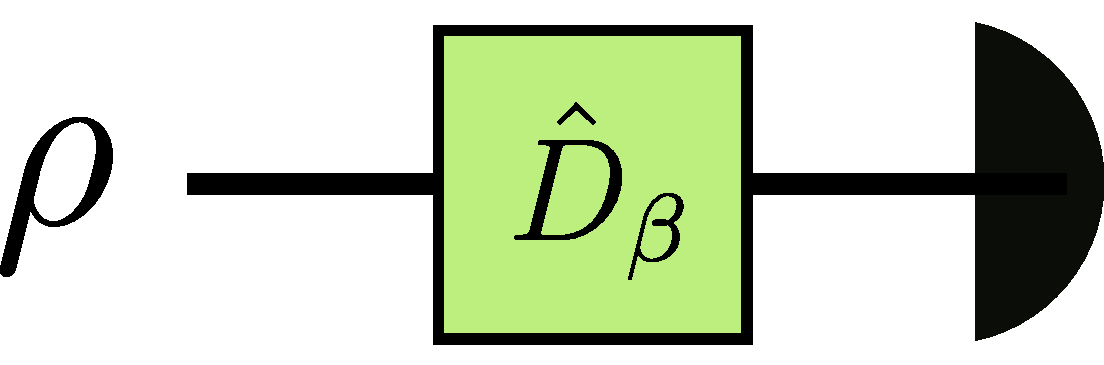
\includegraphics[width=0.5\textwidth]{Figures/312/kennedy_receiver.pdf}
    \caption{We show the Kennedy receiver, which in the case of coherent states' intensity being $\alpha$, it reduces to $\beta = -\alpha$.}
    \label{fig:kennedy_receiver}
\end{figure}

Let us understand the logic behind this receiver. Once displaced, the signal can either be $\ket{0}$ or $\ket{2\alpha}$. In the former case, when measuring with an on/off photodetection --- and in the absense of errors such as dark-counts --- the only possible result is $n=0$ photons. Thus, if outcome $n=1$ was obtained, we can be sure that the signal is $\ket{\alpha}$. However, outcome $n=0$ does not imply that the signal is $\ket{-\alpha}$ with absolute certainty, since $|\braket{0}{2\alpha}|^2 = e^{-4|\alpha^2|}\neq0$. This leads us to evaluate the success probability of Kennedy receiver as:
\begin{align}\label{eq:ps_ken}
P_s^{\text{ken}}(\alpha) = 1 - \frac{e^{-4|\alpha|^2}}{2}.
\end{align}
When compared with the homodyne measurement (\textit{i.e.} Eq.~\ref{eq:gaussian_receiver_homo}), we observe that an advantage in favour of Kennedy receiver is only attained when $|\alpha| \gtrsim 0.4$.

As it happens in cases where little resources are available, each component of a protocol should be optimized if possible. Here, we can readily observe that the displacement value $\beta=\alpha$ might not be the best choice.

\subsubsection{Optimized Kennedy receiver}
By identifying the displacement as a degree of freedom to be optimized, we have $\textit{parametrized}$ the Kennedy receiver, and its performance is now measured by the success probability associated to the specific choice of $\beta$. For a fixed $\beta$, we will denote such receiver as the $\beta$-Kennedy receiver (the original Kennedy receiver is recovered for $\beta = \alpha$).

We note that different values of $\beta$ will lead to different POVMs $\mathcal{M}_\beta$, each belonging to the same family of Kennedy-like receivers. This is analogous to the case of parametrized quantum circuits studied in Sec.~\ref{sec:1_nisq}, in which a unitary transformation was constructed from local qubit rotations and entangling CNOT gates, and optimized in such a way to minimize a given cost function. From this quantum machine learning point of view, the parametrized quantum circuit analogous is given by $\mathcal{M}_\beta$ and the success probability (or, equivalently, the error probability) $P^{\beta-\text{ken}}_e(\alpha, \beta)$ plays the role of the cost function.

Depending on the context, this problem also falls into the category of \textit{optimal control theory}~\cite{Bell1964, Bert05}, since one is interested in optimizing the cost function. This field tries to find answers on how to steer a system towards a target state by performing external controls or \textit{actions} on it. For instance, such system can be thought as our coherent state $\ket{\alpha^{(k)}}$, whose phase needs to be deciphered by the $\beta$-Kennedy receiver, and different actions correspond to varying the value of $\beta$. In this regard, navigating through the optimization landscape is important in order to find which actions are the best, though doing so is generally hard. For instance, one needs to estimate the cost value for each possible value of the control: in our discrimination example, this means estimating the success probability associated to each possible $\beta$-Kennedy receiver out of several repetitions of the discrimination experiment. While estimating the entire landscape is generally too costly, we can get some insight into the problem at hand by studying simplified models. In particular, certain scenarios can readily be deemed \textit{hopeless}, in the sense that parameter optimization might only succeed with an exponentially vanishing success probability, as it happens with barren plateaus appearing in certain parametrized quantum circuits (see  Sec.~\ref{sec:1_nisq})

\begin{figure}[t!]
    \centering
    \includegraphics[width=.9\textwidth]{Figures/kenn_landscape.pdf}
    \caption{We show the optimization landscape for the $\beta$-Kennedy receiver, at a fixed intensity $\alpha=0.2$. which in the case of coherent states' intensity being $\alpha$, it reduces to $\beta = -\alpha$.}
    \label{fig:optiland}
\end{figure}

In this chapter, the simplified model that allows us to get some insight is precisely the $\beta$-Kennedy receiver, whose optimization landscape is shown in Fig.~\ref{fig:optiland} for a fixed value of $\alpha=0.2$. In this a region, the homodyne receiver outperforms the Kennedy one, as noticed after inspecting Eq.~\ref{eq:ps_ken}. However, we observe that there is an entire region of $\beta$ values for which the $\beta$-Kennedy receiver can actually surpass the homodyne limit. Note also that the optimal solution is degenerate; this is a consequence of the symmetry in testing either $\ket{\alpha}$ (negative $\beta$) or $\ket{-\alpha}$ (positive $\beta$) using the photon-detector logic explained above.

\begin{figure}[t!]
\centering
    \begin{subfigure}[b]{0.49\textwidth}
        \centering
        \includegraphics[width=1.\textwidth]{Figures/312/kennedy_compa.pdf}
    \end{subfigure}
    \hfill
    \begin{subfigure}[b]{0.49\textwidth}
        \centering
        \includegraphics[width=1.\textwidth]{Figures/312/kennedy_compa_diff_hel.pdf}
    \end{subfigure}
\caption{We compare the success probabilities for homodyne receiver, Kennedy receiver, and optimized-Kennedy receiver with the Helstrom bound. Data in both panels is the same, however in right one we show the different with Helstrom bound, in order to help visualization.}
\label{fig:kenn_compa1}
\end{figure}

In this way, the optimization over $\beta$ can be carried out for each value of $\alpha$. The resulting receiver is known as the \textit{optimized Kennedy receiver}, and surpasses the homodyne limit for all intensity values, as shown in Fig.~\ref{fig:kenn_compa1}, where we compare its success probability, denoted by $P_S^{opt-\text{ken}}$, with that of homodying and with the original Kennedy receiver $P_S^{\text{ken}}$ (\textit{e.g.} $\beta = -\alpha$). To aid the comparison, we have depicted the difference with respect to the Helstrom bound: how to approach such a limit is the matter of the next section.

%

\subsection{Dolinar receivers}\label{ssec:rlcoh_dolinarreceiver}
Sequential strategies lie in the heart of this thesis, and this Chapter is no exception. The Dolinar receiver~\cite{Dolinar1973} is a concatenation of $\beta$-Kennedy receivers, each acting on an tiny portion of the original signal.

In particular, this receiver consists on splitting the incoming coherent state by using beam-splitters (BMs), resulting into $L$ lower-intensity copies, \textit{e.g} $\ket{\alpha_k^{(\ell)}} = \ket{\frac{\alpha_k}{\sqrt{L}}}$ for $\ell=1,...,L$. From here, the phase of each state is tested by using a $\beta$-Kennedy receiver. Crucially, a sequential logic is applied, in which the displacement value at $\ell$-th stage depends on the measurement outcomes previously obtained, as shown in Fig.~\ref{fig:313dolinar_setup}. This conditioning operation is known as a classical feed-forward, and should in principle be optimized over all possible measurement outcomes.
\begin{figure}[t!]
    \centering
    \includegraphics[width=.8\textwidth]{Figures/313/dolinar_receiver.pdf}
    \caption{We show a Dolinar-like receiver. For an infinite sequence measurements and feedforward operations, such a scheme attains the Helstrom bound for binary coherent-state discrimination.}
    \label{fig:313dolinar_setup}
\end{figure}
We note that for $L=1$ we recover the optimized-Kennedy receiver. However, because of its structure consisting on $L$ processing \textit{layers} $\ell=0,\cdots,L$, Dolinar receiver is considerably more complex than the Kennedy one. Specifically, for each layer $\ell<L$, the following operations are applied:
\begin{enumerate}
\item The input signal $\ket{\alpha}$ (or equivalently $\ket{-\alpha}$) is split on a BS of transmissivity $\theta$, effectively extracting a fraction $1-\theta$ of the energy for detection. The BS transforms the input signal and vacuum states as
\begin{equation}
\ket{\alpha}\ket{0}\mapsto\ket{\alpha\sqrt{\theta}}_{\rm tr}\ket{\alpha\sqrt{1-\theta}}_{\rm ref},
\end{equation}
Note that the BS adds a phase to the second mode, which we assumed corrected via a proper phase-shifter not shown in the figure.
\item The reflected part of the signal undergoes a displacement operation $\Dis{\beta}$. Such operation is realizable via interference with a strong coherent signal on a small-reflectivity BS, not shown in the figure. The resulting state is $\ket{\tilde{\alpha}(\beta,\theta)}_{\text{ref}}=\Dis{\beta}\ket{\alpha\sqrt{1-\theta}}_{\text{ref}}$.
\item\label{ops:end} The displaced signal is measured via a on/off photodetector, which detects no photon, i.e., outcome $o_{\ell+1} = 0$, with conditional probability
\begin{equation}\label{eq:313singLayProb}
p(o_{\ell+1}=0|\alpha,(\beta,\theta))=\abs{\braket{0}{\tilde{\alpha}(\beta,\theta)}_{\text{ref}}}^{2}=e^{-\abs{\tilde{\alpha}(\beta,\theta)}^{2}},
\end{equation}
and detects one or more photons, i.e., $o_{\ell+1}=1$, with probability $1-p(o_{\ell+1}=0|\alpha,(\beta,\theta))$.
\item The transmitted part of the signal enters layer $\ell+1$.
\end{enumerate}
Finally, the last processing layer $\ell=L$ consists in elaborating a guess $\hat{k}$ of the true hypothesis $k$, based on previous measurement outcomes and parameter choices.

Similar to $\beta$-Kennedy receivers, Dolinar-like receivers are parametrized by the displacements $\Dis{\beta}$. Nevertheless, the complexity is considerably higher: while $L$ displacement operations should be performed per signal detection, the feed-forward conditioning non-trivally enlarges the optimization landscape to $2^{L}-1$ possible values.

In addition, we shall now adopt the control-theory mindset introduced in Sec.~\ref{sec:1_rl},%\footnote{We will indistinctly talk about optimal control theory and reinforcement learning, while both fields come from different communities, they are faces of the same coin.} introduced in Sec.~\ref{ssec:rlcoh_kennedyreceiver}. Here,
and think of the displacements $\Dis{\beta_\ell}$ and attenuations $\theta_\ell$ as \textit{actions} $a_{\ell}$ performed on the signal.

Under these definitions, let us now study the success probability associated to a Dolinar-like receiver. For an initial coherent state $\ket{\alpha}$, the input state at the $\ell$-th layer is $\ket{\alpha_{\ell}}=\ket{\alpha\sqrt{\theta_{0}\cdots\theta_{\ell-1}}}$. In principle, we can use all the past history defined as
\equ{h_{\ell}=(a_{0},o_{1},\cdots,a_{\ell-1}),}
with $h_{0}=\emptyset$, to decide the next value of $(\beta,\theta)$ and the final guess. We label them compactly as $a_\ell(h_{\ell})=(\beta_{h_{\ell}},\theta_{h_{\ell}})$ and $a_{L}(h_{L})=\hat{k}$, omitting the label $\ell$ or the dependence on $h_{\ell}$ when it is clear from the context.

Hence, the average success probability of the $L$-Dolinar receiver, \textit{calibrated} under actions $\{a_\ell\}$, and averaged out over all possible outcomes' sequences $o_{1:L}=(o_{1},\cdots,o_{L})$ can be written as
\begin{equation}\label{eq:psdol}
P_{s}(\alpha,\{a_\ell\})=\sum_{o_{1:L}} \prod_{\ell=1}^{L}p(o_{\ell}|\alpha^{(k)},a(h_{\ell})) \; p_{k}\Big|_{k=a(h_{L})},
\end{equation}
Here, the configuration $\{a_{\ell}\}$ is the total set of actions over all histories, and we have written the conditional probability of the sequence of outcomes $o_{1:L}$ as a product of single-layer conditional probabilities, \textit{e.g.} Eq.\eqref{eq:313singLayProb}. In particular, we aim to optimize this success probability over the available actions of the receiver, and this value will denote as
\begin{equation}\label{eq:32OptSuc}
  P_{*}^{(L)}(\alpha) = \underset{\llaves{a_{\ell}}}{\text{ max }} P_s(\alpha, \llaves{a_\ell}).
\end{equation}
We will omit the dependence on $L$ whenever it is clear from the context.

The importance of the Dolinar receiver is that \textit{it is known to attain the Helstrom bound} in the limit of many layers, \textit{i.e.} $L\rightarrow \infty$, provided that the optimal actions are performed. However, before discussing such optimality and the structure of the receiver further, we will comment on an alternative formulation of this receiver.

\subsection{Time-domain Dolinar receiver $\&$ optimality}\label{ssec:tdol}
\begin{figure}[t!]
    \centering
    \includegraphics[width=1.\textwidth]{Figures/dolianr_cont.png}
    \caption{We show the original proposal of the Dolinar receiver, which works in continuous-time. This image is taken from Ref.~\cite{revisiting2011Assalini}. Instead of splitting the coherent-state in space by a beam-splitter array, we here have the signal spread in time, as explained in the main-body. The $\ell$-dependence in the conditional displacements is now translated into a time-dependence for $u(t)$, which in turn depends on the parity of the measurement outcomes as captured by the function $z(t)$. After the pulse-duration $T$, a decision for the phase of the coherent state is done via the function $z(T)$.}
    \label{fig:dolinar_cont}
\end{figure}
While we have introduced Dolinar receiver in the spatial-domain, its original formulation was done in the continuous-time domain~\cite{Dolinar}. The two formulations are related to each other by the equivalence between continuous-time photon-counting procesess and a (sufficiently-large) sequence of lossless beam-splitters and photon-detectors, as shown in Ref.~\cite{quasicontinuous}.

In the time-domain picture, the coherent state $\ket{\pm \alpha}$ is understood as a travelling-mode, and given by the field $\psi(t) = \pm \psi e^{\ii \omega t}$, where $\omega$ is the optical frequency and $|\alpha|^2 = \int_0^T |\psi(t)|^2dt = \psi^2 T$, with $T$ the total duration of the pulse. At each time $t$, the receiver shifts the incoming-field by a value $u_{z(t)}(t)$, and measures it by a photon-detector, as depicted in Fig.~\ref{fig:dolinar_cont}. Such measurement is assumed to be carried out very fast, leading only to binary outcomes (click or no click), which defines a so-called
\textit{compound Poisson process}. As shown in Dolinar's PhD thesis, the most-likely hypothesis $k$ is given by the parity of the sum of the outcomes obtained up to time $t$, and this determines the binary value $z(t)$ that controls the nature of the displacements to be done at consecutive times. The optimal shape of the pulses $u_{z(t)}(t)$ and of the success-probability of this scheme was originally derived in Ref.~\cite{Dolinar} by performing a dynamic programming optimization of the likelihood-ratio; in turn, he was able to show that the receiver attains the Helstrom bound. %However, following his approach can be painful, and we refer the interested reader to Refs.~\cite{Geremia2004,revisiting2011Assalini} for more compact proofs of the optimality.

In this line, the optimality of Dolinar receiver can also be proved in the spatial-domain (\textit{e.g.} the array of beam-splitters and conditional displacements) as follows. With sufficiently many measurement layers, say $L$, the coherent state will be splitted into $L$ copies, each having a very low intensity. From here, we can recall the results of Ref.~\cite{Acin2005Multi}, namely that the optimal discrimination between multiple copies of two pure quantum states can be achieved by a sequential strategy, in the assymptotic case of many copies. This strategy consists on a local projective measurement that is optimized at each step according to the most likely hypothesis; most notably the global measurement optimization problem is solved by an adaptive-local measurement, which hinges on bayesian updating the prior probabilities of each hypothesis after each measurement result. Such strategy is shown to achieve the Helstrom bound, and it can readily be applied to the $L$ copies of the attenuated coherent-state. In Ref.~\cite{revisiting2011Assalini} it was shown that, following this approach, the optimal adaptive measurement coincides with the Dolinar receiver, in the binary coherent-state discrimination problem. Also, let us mention that an alternative proof of Dolinar receiver's optimality is given in Ref.~\cite{Takeoka2005}

\bigskip
However, in practical experimental scenarios it is not possible to perform a large number of measurement layers. Such constraint is justified by \textit{(i)} the experimental feasibility of constructing the receiver, and \textit{(ii)} the noise accumulation at every layer.

Moreover, noise might even accumulate with the number of layers, as it happens with one of the most common sources of photon-detectors noise, the dark counts. Here, a click appears in the detector even when measuring the vacuum. Moreover, optimality of Dolinar receiver also requires the feed-forward operation to act before the signal reaches the next measurement layer. However, measuring and classical post-processing do take some time, and this delay is in practice modelled by including losses in between each measurement layer~\cite{sychLeuchs}.

From our previous discussion, it might seem that we are heading towards a paradigm where a set of suggestions is given to the experimentalist, with the optimizing actions in Eq.~\ref{eq:32OptSuc} essentially constituting the recipe to follow. This paradigm is actualy followed in Chapter~\ref{chapter:VANS}, where several cost-minimizing quantum circuits are discovered using our VAns algorithm, which is shown to work under several noise-models. While our experimental simulations should be realistic as possible, the usefulness of the recipe we provide will ultimately depend on how accurate can reality be modeled.

On the contrary, we will here tackle the situation from a different angle, and adapt to reality on the fly. This is the radical and experimentally-centered approach taken in this Chapter. To this end, a reinforcement-learning agent is faced towards the discrimination experiment, and asked to optimize its Dolinar-like receiver by having only access to an answer: \textit{yes/no}, a binary value standing for the correctness of its guess.

\subsection{The sequential structure of Dolinar receiver}\label{ssec:3bis_intuition}
Before jumping to the optimization of Dolinar-like receivers (either model-aware or model-free), it is important to further discuss its structure, as captured by Eq~\ref{eq:psdol}. In turn, we can take profit of the sequential structure, in order to compute Eq.~\ref{eq:32OptSuc} in a model-aware setting, a quantity that will help us to benchmark the performance of agnostic agents.

We will refer to a finite Dolinar receiver, \textit{i.e.} one consisting on $L$ processing layers as \textit{$L$-Dolinar}, and refer to the prior probability of having the state $\ket{+\alpha}$ as $\eta_0 = \eta$; as a consequence the prior probability of $\ket{-\alpha}$ is $\eta_1 = 1-\eta$. Whenever it is clear from the context, we will drop the subscripts and simply refer to $\eta$.

To this end, we will study the performance of the $L$-receiver layer by layer, and first consider a $0$-Dolinar receiver. Without any measurement, we only rely on the prior probabilities to asses the label of the states (\textit{e.g.} to guess for the value of $k$). The success probability of such a trivial receiver thus corresponds to the probability of the most likely hypothesis:
\begin{equation}\label{eq:0dol}
P_s^{L=0}(\alpha, \eta) = \text{max } \llaves{\eta, 1-\eta}.
\end{equation}
Let us now consider an $1$-Dolinar receiver (\textit{e.g.} a Kennedy-like receiver). In such a case, the success probability --- when considering the optimal, \textit{i.e.} maximum-likelihood guess--- reads
\begin{align}\label{eq:1dol}
P_s^{L=1}(\alpha, \llaves{a}, \eta) &= \sum_{o_1 = 0,1} \underset{k}{\text{max }} p(\alpha_k, o_1),
\end{align}
where $p(\alpha_k, o_1)$ denotes the joint probability of having the state $\ket{\alpha_k}$ and observing outcome $o_1$, and $\llaves{a}$ reduces to the displacement with value $\beta$, as shown in Fig.~\ref{fig:kennedy_receiver}.

The joint probability $p(\alpha_k, o_1)$ can be written in terms of the prior probabilty $\eta_k$ of having $\ket{\alpha_k}$ times the probability of observing outcome $o_1$, given we actually have such state:
\begin{align}\label{eq:1dol_eta}
P_s^{L=1}(\alpha, \llaves{a}, \eta) &=\sum_{o_1 = 0,1} \underset{k}{\text{max }} p(o_1 | \alpha_k) \eta_k.
\end{align}
On the other hand, we can also write the joint probability in terms of the total outcome probability, \textit{i.e.} $p(o_1) = \sum_{k} p(o_1, \alpha_k ) = \sum_{k} p(o_1|\alpha_k ) \eta_k$, and the \textit{posterior} probability of having $\ket{\alpha_k}$ once $o_1$ was observed:
\begin{equation}\label{eq:rlcoh_bayes_prior}
\eta_{k|o_1} = p(\alpha_k | o_1) = \frac{p(o_1|\alpha_k ) \eta_k}{p(o_1)}.
\end{equation}
With this, the success probability of Kennedy-like receivers reads
\begin{align}\label{eq:1dol_post}
P_s^{L=1}(\alpha, \llaves{a}, \eta) &=\sum_{o_1 = 0,1} p(o_1)\;\underset{k}{\text{max }} p(\alpha_k| o_1) \\
&=\sum_{o_1 = 0,1} p(o_1) \;P_s^{L=0}(\eta_{k|o_1}),
\end{align}
where the dependence on $\llaves{a}$ is left implicit. We note that once once the outcome is observed, 1-Dolinar receivers trivially recurs to 0-Dolinar receivers, with a bayesian-updated prior values.

Let us now consider a 2-Dolinar receiver. Here, the success probability reads
\begin{align}\label{eq:2dol}
P_s^{L=2}(\alpha, \llaves{a}, \eta) &=\sum_{o_1 = 0,1}\sum_{o_2 = 0,1} \;\underset{k}{\text{max }} p(\alpha_k, o_1, o_2) \\
&=\sum_{o_1 = 0,1}\sum_{o_2 = 0,1} p(o_1, o_2)\;\underset{k}{\text{max }} p(\alpha_k|o_1, o_2 )\\
&=\sum_{o_1 = 0,1} p(o_1) \sum_{o_2 = 0,1} p(o_2|o_1)\;\underset{k}{\text{max }} p(\alpha_k|o_1, o_2 )\\
&=\sum_{o_1 = 0,1} p(o_1) \sum_{o_2 = 0,1} p(o_2|o_1)\;\underset{k}{\text{max }} \frac{p(o_2| \alpha_k o_1) \;p(\alpha_k|o_1)}{p(o_2|o_1)}\\
&=\sum_{o_1 = 0,1} p(o_1) P_s^{L=1}(\eta_{k|o_1}),
\end{align}
where we expressed conditional outcomes probabilities as $p(o_1, o_2) = p(o_2|o_1)p(o_1)$, and used
\begin{equation}\label{eq:depend}
p(o_2|o_1) = \sum_{k}p(o_2 \alpha_k|o_1) = \sum_k p(o_2|\alpha_k o_1) p(\alpha_k|o_1) = \sum_k p(o_2|\alpha_k o_1) \eta_{k|o_1}.
\end{equation}
Here, we can readily highlight the conditional dependence of the actions. In the 2-Dolinar receiver, they are given by $\llaves{a_1, a_2^{o_1=0}, a_2^{o_1=1}}$, where $a_1$ denotes the first displacement (which is unconditional) and $a_2^{o_1}$ stands for the second displacement (conditioned on the outcome $n-1$). While this can be extended to consider the attenuation values as well, we will not reinforcement-learn them, since their contribution to the success probability is very small, as observed in the next Section.

Thus, the conditional dependence of the actions is reflected in the outcome probabilities. For the first outcome $o_1$, the dependence is only on $a_1$ as
\begin{equation}
p(o_1) = \sum_k p(o_1 \alpha_k) = \sum_k p(o_1|\alpha_k) \eta_k = \sum_k (o_1 + (-1)^{o_1} e^{-|\alpha_k + a_1|^2})\eta_k,
\end{equation}
where we have wrote compactly the outcome probability of an on/off photodetector with coherent state $\ket{\alpha_k + a_1}$ as input. Furthermore, as Eq.~\ref{eq:depend} indicates, the dependence of $o_2$ with $o_1$ has a contribution on $a_2^{o_1}$ (through $p(o_2|\alpha_k o_1)$), but also through the updated prior $\eta_{k|o_1}$. In turn, the sequential interpretation of the Dolinar receiver crucially depends on this bayesian update; as observed in Eq.~\ref{eq:2dol}, a $2$-Dolinar receiver is an extension of a $1$-Dolinar receiver, in which the prior probability of each hypothesis is modified according to the first measurement outcome.

Similarly, the sequential structure can be made explicit for the $L$-Dolinar receiver. Let us denote with $o_{\ell_1:\ell^{'}}$ the string of outcomes $(o_{\ell_1}, o_{\ell_1 +1}, ... o_{\ell_{'}})$ (with $\ell < \ell^{'}$). Then, the success probability of $L$-Dolinar receiver reads
\begin{align}\label{eq:Ldol}
P_s^{L}(\alpha,\eta) &= \sum_{o_{1:L}}  \underset{k}{\text{max }} p(\alpha_k, o_{1:L})  \\
&= \sum_{o_1} p(o_1) \sum_{o_{2:L}} p(o_{2:L}|o_1)\underset{k}{\text{max }} p(\alpha_k| o_{1:L}) \\
&= \sum_{o_1} p(o_1) \sum_{o_{2:L}} p(o_{2:L}|o_1)\underset{k}{\text{max }} \frac{p(\alpha_k| o_{2:L})\; p(\alpha_k| o_{1})}{p(o_{2:L}|o_1)} \\
&= \sum_{o_1} p(o_1) \sum_{o_{2:L}} \underset{k}{\text{max }} p(\alpha_k| o_{2:L})\; p(\alpha_k| o_{1}) \\
&= \sum_{o_1} p(o_1) P_s^{L-1}(\eta_{k|o_1}).
\end{align}
Thereby, enlarging Dolinar's receiver with an extra layer translates into bayesian updating the prior probability of each hypothesis.

This resemblences to the dynamic programming procedure we discussed in Sec.~\ref{ssec:1_rl_dp}, where the principle of optimality (\textit{i.e.} the recurrence relation given by the optimal Bellman equation) allowed us to sequentially attain the optimal policy. Here, we observe that the best success probability --- \textit{i.e.} that optimized over all actions $\llaves{a}$ --- can be obtained by a sequential optimization of local problems, in this case given by Kennedy-like receivers with varying priors.

Before jumping to this model-aware optimization, let us highlight some further symmetries that will find use in the following section. In particular, note we that the prior probability of having $\ket{\alpha}$, \textit{e.g.} $\eta_0 = \eta$, is sufficient to encode all the information required for the binary discrimination problem, since $\eta_1$ is trivially be obtained from $\sum_k\eta_k=1$. This simple symmetry should also be translated into the success probability. In turn, from Eq.~\ref{eq:1dol_eta} it is trivial to see that
\begin{align}\label{eq:symmetry_kenn}
P_S^{L=1}(\eta, \llaves{a}) =  P_S^{L=1}(1-\eta, \llaves{-a}),
\end{align}
where by $-a$ we mean that the displacement take now the opposite values. In practice, since $\eta_k \in[0,1]$, this means that it is sufficient to consider half of such an interval, the complementary optimal actions can be obtained from Eq.~\ref{eq:symmetry_kenn}.

We will now turn to explain how the sequential structure studied above can be exploited in order to compute the optimal values of the displacements and success probabilities in the fully-aware scenario.
% Moreover, this symmetry is trivially extended to the probability $p(n)$, and hence we can also use it for optimizing $L$-Dolinar receivers, which is the matter of the next section.% Sec.~\ref{sec:rlcoh_model_aware_approach_intro}.


\section{The model-aware approach}\label{sec:rlcoh_model_aware_approach_intro}
We will now discuss the model-aware optimization of Dolinar-like receivers, which is based in the observations outlined previously regarding the sequential structure of such receivers.

As introduced in Sec.~\ref{ssec:1_rl_dp}, dynammic programming exploits the so-called principle of optimality, which links optimal actions to optimal state value functions through the optimal Bellman equation, see Eq.~\ref{eq:vBellOp}. In there, we introduced Markov Decision Problems (MDP) consisting on an agent that sequentially interacts with its environment in order to maximize a figure of merit known as the return. This quantity captures the amount of rewards the agent collects during an episode, and it here translates to the correcteness of agent's guess, which is obtained after measuring the state by a Dolinar-like receiver. In the MDP section, we have also made the distinction between agent and environment states, which arises due to the impossibility of the agent to have fully access to the environment's state at a given step, and thus Partially Observable Markov Decision Processes were introduced. Here, we will define the environment states as the underlying quantum states $\ket{\alpha_k}$ to be discriminated.

\begin{figure}[t!]
    \centering
    \begin{subfigure}[b]{0.49\textwidth}
        \centering
        \includegraphics[width=1.\textwidth]{Figures/314/34_dp_results.pdf}
        \caption{}
        \label{fig:dpre1}
    \end{subfigure}
    \begin{subfigure}[b]{0.49\textwidth}
        \centering
        \includegraphics[width=1.\textwidth]{Figures/314/paper_dp_results_notation.png}
        \caption{}
        \label{fig:dpre2}
    \end{subfigure}
    \caption{We show the difference between the best probability of success attainable for a fix $L$ and the optimal probability of success in discriminating BPSK coherent states. The results were obtained by dynamic programming. \textit{Left panel}: the attenuations at the beam-splitters are fixed in such a way that each partial measurement deals with a state having the same intensity $\alpha^{\ell}_k=\frac{\alpha_k}{\sqrt{L-1}}$ for all $\ell$. \textit{Right panel}: we compare the advantage of adapting beam-splitter transmisivities (dashed lines) as compared to the receivers considered in left panel (solid lines).}
    \label{fig:dp_resu}
\end{figure}

Since in the model-aware scenario the agent has full access to the outcomes probabilities, it is sensible to define agent's state as the prior probability of $\ket{\alpha_k}$ at each layer of the receiver. Intuitively, such a quantity stands for the belief distribution over the states $\ket{\alpha_k}$, and it is defined as:
\begin{align}\label{eq:belief}
b_{\ell}(k) = p(\alpha^{(k)}_{\ell}|o_{\ell},a_{\ell-1},b_{\ell-1}).
\end{align}
As new information about the hidden state is collected, the belief evolves. The evolution law of this quantity is obtained by a bayesian update, which reads:
\begin{eqnarray}\label{eq:belUp}
b_{\ell}(k) = \frac{p(\alpha^{(k)}_{\ell}|o_{\ell}, a_{\ell-1}) \;b_{\ell-1}(k)}{\sum_{k} p(\alpha^{(k)}_{\ell}|o_{\ell}, a_{\ell-1}) \; b_{\ell-1}(k)}.
\end{eqnarray}
We can readily define the state value function $v(s)$, recalling it quantifies how \textit{valuable} state $s$ is in terms of the expected return. In our case, the return reduces to the final reward obtained after action $a_L$, \textit{e.g.} guessing, and the expected return becomes the success probability associated to agent's policy. Specifically, agent's policy consists on specifying the actions of its $L$-Dolinar receiver, and we are thus interested in finidng the optimal policy, which on the one hand is linked to Eq.~\ref{eq:32OptSuc}, and on the other hand its state value function should satisfy the optimal Bellman equation.% (\textit{e.g.} Eq.~\ref{eq:vBellOp}).

To understand this last point, let us consider final last step of an $L$-Dolinar receiver, which consists on performing a guess. The optimal action to take is the maximum-likelihood guess, and its associated value function reads
\begin{equation}\label{eq:opBellLQSD}
v^{*}_{L}(b_{L})= \max_{k} b_{L}(k).
\end{equation}
Observe that since $\sum_k b_\ell(k)=1$, it is sufficient to track $b_\ell(k=0)$. The optimal Bellman equation at step $\ell<L$ instead reads
\begin{equation}\label{eq:opBellEllQSD}
v^{*}_{\ell}(b_{\ell})=\underset{a\in\mathcal{A}(s_{\ell})}{\text{max }} \sum_{o_{\ell+1}\in\mathcal{O}} \sum_k p(o_{\ell+1}; b_\ell(k), a_\ell)v^{*}_{\ell+1}(b_{\ell+1}).
\end{equation}
% \begin{equation}\label{eq:opBellEllQSD}
% v^{*}_{\ell}(b_{\ell})=\underset{a\in\mathcal{A}(s_{\ell})}{\text{max }} \sum_{o_{\ell+1}\in\mathcal{O}} \sum_k p(o_{\ell+1}|\alpha_k,a_\ell) b_{\ell}(k)v^{*}_{\ell+1}(b_{\ell+1}).
% \end{equation}

%
% Hence, by computing optimal state-value functions in a recurrent and backward fashion, we are able to find optimal actions for $L$-Dolinar receivers. Specifically, we depart from the final layer ($\ell = L$), and compute the state-value function for a discrete amount (but sufficiently many) of belief values. Note that because of the symmetries highlited in Sec.~\ref{ssec:3bis_intuition}, we can restrict to the interval $\mathcal{B} = \left[0,\frac{1}{2}\right]$, which essentially stands for agent's state space $\mathcal{S}$ of this problem.
The last equation shows that the value-functions can be computed \textit{back-wards}. In this sense, we can first compute the optimal state-value functions for the final layer, then move the previous layer (\textit{i.e.} $\ell = L-1$), and compute optimal ones using Eq.~\eqref{eq:opBellEllQSD} for each belief value in a (discretized) set of possible beliefs $\mathcal{B}$. Because of the symmetry highlighted in Eq.~\ref{eq:symmetry_kenn}, we can consider points in between the interval $[0,\frac{1}{2}]$.

However, we note that for a given $b_\ell \in \mathcal{B}$, the posterior probability $b_{\ell+1}$ appearing in optimal Bellman equation might lie outside the set $\mathcal{B}$. This constitutes a problem, since its state value function is unavailable from the previous step. To circumvent this issue, we interpolate $v_{\ell+1}^*(b)$ to the entire interval $[0,1]$ using Eq.~\ref{eq:symmetry_kenn}, and to this end we require many points in $\mathcal{B}$ (in our numerics we considered $100$).

% Moreover, note that the success of this procedure hinges on the fact that the \textit{optimal} value function was computed, and thus assumes the actions can be optimized correctly. Nevertheless, such optimization can find difficulties. For instance, values of the belief that are close to the extremal points (\textit{e.g.} $0$ or $1$), the optimization landscape flattens, since the success probability already approaches to $1$, and each layer can only contribute with a very small percentage to increase the success probability. Note that such small contributions are actually important, since Dolinar-like receivers assymptotically approach to the Helstrom bound, and thus optimizing such points becomes crucial for large values of $L$. On the other hand, the optimization landscape can present difficulties in the presence of noise, a situation we will discuss below.

% \begin{figure}[b!]
%     \includegraphics[width=.45\textwidth]{Figures/314/dolinar_receiver_with_theras_adaptive.pdf}
%     \caption{We show an enhanced Dolinar-like receiver, where Beam-Splitter transmisivity values are also conditioned on previous measurement outcome}
%     \label{fig:dolinar_with_attas}
% \end{figure}

In our numerics, shown in Fig.~\ref{fig:dp_resu} we were able to optimize up to $L=30$; the interpolation method is based on Radial Basis Functions (see \textit{e.g.} introduction of Ref.~\cite{rbf_interpolate}) and the minimization method used was dual annealing~\cite{scipy}. Moreover, following a similar proccedure than outlined above, we can optimize over the attenuations as well. The latter proves advantageous, since from $L=4$ and on, adaptive beam-splitters outperform non-adaptive ones, even in the case where an extra layer is included for the latter. To see this, consider Fig.~\ref{fig:dp_resu}: we observe that dashed lines (adaptive beam-splitters) for $L=5$ outperform solid ones (non-adaptive beam-splitters) even for $L=6$.
% As previously pointed out, making use of noisy quantum devices is a tricky task. Here, in order to mitigate the effects of noise, one needs to optimize each possible component of the apparatus. When it comes to Dolinar receivers, there is an additional degree of freedom we have not exploited yet, which is related to the way that the incoming signal is splitted. In particular, the success probability also depends on Beam-Splitters' attenuations, and we could in principle optimize them as well. Thus, we could think on a scheme as the one depicted in Fig.~\ref{fig:dolinar_with_attas}, where the measurement outcome not only conditiones the displacement value, but also the transmissivity of the next BS, which acts on the remaining part of the signal. While conditioning the displacement value according to the measurement outcome can be carried out relatively fast~\cite{Becerra2013,Cook2007}, it is unclear whether we have the technology required to condition transmisivities in a fast way. Nevertheless, we have carried out these numerics which indicate that,

\subsubsection{Unveiling Dolinar's strategy from the numerics}
\begin{figure}[t!]
    \centering
    \includegraphics[width=1.\textwidth]{Figures/strat_dolinar.pdf}
    \caption{\small{We show the structure of the optimal policy for a $10$-Dolinar receiver, where we consider $\alpha=0.4$. Each panel corresponds to a different string of observations obtained through a possible experiment realisation. At each layer, the optimal policy obtained through dynamic programming instructs the agent to perform an action (a displacement) according to the current belief $b_\ell$ on state $\ket{\alpha}$; such belief is updated as more information about the environment state is acquired. Thus, in order to obtain this plot, we propagate the initial prior (set to $\frac{1}{2}$) as per Eq.~\ref{eq:belUp}, using the corresponding measurement outcome. Then, we find the interpolate the optimal action that corresponding to that belief, and repeat this along the $10$ layers. Here, we do also compute the total probability of finding each sequence, as per $p(o_{1:L}) = \sum_k p(o_{1:L}|\alpha_k)\eta_k$. Such probability is extremely low for the rightmost sequence (all ones), here rounded to zero, and considerably high for the sequence of all zero outcomes (see discussion in the main body).}}
    \label{fig:strategy_dp}
\end{figure}
\afterpage{\clearpage}

It is worth discussing the optimal strategy, \textit{i.e.} which are the displacements obtained of each layer after the dynamic programming optimization for a fixed $L$. In Fig.~\ref{fig:strategy_dp} we illustrate this optimal strategy, for the $10$-Dolinar receiver. Here, we do only consider a subset of the $2^{10}$ possible combinations of measurement outcomes that can be observed in a single discrimination experiment.

As with Kennedy receiver, Dolinar one is equipped with on/off photodetectors, which projects the incoming state either into the vacuum $\proj{0}$ (no photons), or into its complement $\mathbb{I} - \proj{0}$ (one or more photons). Displacing the signal by $\beta$ right before such measurement acts as a projection $\proj{\beta}$ (or $\mathbb{I}-\proj{\beta}$), and as outlined in Sec.~\ref{ssec:rlcoh_kennedyreceiver} there is a symbiosis between displacements and photon-detection that surpasses the so-called \textit{homodyne limit}, when optimizing over $\beta$.
While for Kennedy receivers $\beta = \alpha$, leading to measure either $\ket{0}$ or $\ket{2 \alpha}$, optimized Kennedy receivers find a better balance between the two contributions by displcing the signal with differnet value (see Fig.~\ref{fig:kenn_compa1}). However, the bottom line is similar: after displacing by a value $\beta>0$ and measuring, if outcome $0$ was obtained, a bet for $\ket{-\alpha}$ is done, and if outcome $1$ is obtained, $\ket{\alpha}$ is then the most likely hypothesis for which the agent bets.

Dolinar receiver exploits this idea, and carries out partial tests in a sequential way. By splitting the signal into $L$ parts, the receiver essentially has now $L$ copies of the state, each attenuated by a factor $\sqrt{L}$. Thus, until a click is detected (measurement outcome $1$), it proceeds similarly to the Kennedy receiver, \textit{i.e.} by testing if the state was $\ket{-\alpha}$. In this sense, the belief of having such state increases according to the number of $0$'s, as can be seen in the Fig.~\ref{fig:strategy_dp}. We also observe that there is a dependence on the value of $\beta$ with the layer number $\ell$, whereas its sign remains positive. However, if the first measurement result happens to be $1$, the preferred hypothesis flips to $\ket{\alpha}$, since by having performed a positive displacement, that is the most-likely state. From there, Dolinar receiver verifies if such claim holds, by testing on the remaining layers whether the state was $\ket{\alpha}$: this is done by changing the sign of the displacement. In turn, if the state $\ket{\alpha}$
was displaced by a value $\beta<0$, then it is more likely to detect outcome $0$. As we can observe in the Figure, if further outcomes happen to be $0$, then the receiver keeps testing $\ket{\alpha}$ through negative displacements. On the contrary, if outcome $1$ is obtained, the strategy flips again (bottom-left panel). The success of Dolinar receiver hinges on the fact that having sequences containing so many consecutive $1$'s is vanishingly small. In turn, for $\alpha=0.4$, we observe that the probability of encountering such a string of outcomes is as small as $10^{-16}$.

We remark that a similar reasoning for the structure of the optimal controls applies in the time-domain Dolinar receiver (see Sec.~\ref{ssec:tdol}), as discussed in Refs.~\cite{Dolinar, Takeoka2005, revisiting2011Assalini}.

We are now in position to turn agnostic, and introduce our reinforcement-learning agent that adapts the receiver to the measurement outcomes sampled from an unknown probability distribution. In such situation, the agent has no other choice than interacting with the receiver through several repetitions of the discrimination experiment, and thus the methods outlined in this Section cannot be applied.


\section{The model-free approach}\label{sec:rl_coh_model_free}
This Section represents the main contribution of the Chapter, namely the real-time model-free calibration of coherent-state receievers.

Here, the reinforcement-learning agent is asked to optimally-calibrate a $L$-Dolinar receiver, but is provided  with essentially no information about the setting: she can only select actions according to the experience gathered via sequential repetitions of the discrimination experiment.

By the end of each episode (each discrimination experiment), the agent is only given \textit{one bit of information}, \textit{i.e.} the reward that accounts for the correcteness of her guess. Thus, if the agent is able to calibrate the receiver such that it performs near-optimal actions $\llaves{a_\ell}$, then the rewards enjoyed will be higher on average. This stresses the difficulty of the setting proposed: \textit{even if the receiver was calibrated to perform optimally, there is a chance of enjoying no reward}. In turn, the reward is a Bernoulli-distributed random variable with success probabilty $P_s^{L}$, and even the optimal configuration in Eq.~\ref{eq:32OptSuc} will experience a zero reward with probability $1-P_*^{L}$.

% The commented in the introduction of this Chapter, studying the performance of finite Dolinar receivrers (\textit{e.g.} finite $L$) is experimentally justified, whereas the model-free assumption is motivated by communication scenarios where the presence of unknown quantum channels can non-trivially act on the transmitted signal. Thus, our model-free approach finds its roots in Reinforcement Learning, which was discussed previously; in order to apply such ideas to the calibration of this receiver, we will require some definitions, which are given in the following Section.

\subsection{Reinforcement learning the Dolinar receiver}\label{ssec:rl_cohql}
Reinforcement learning was discussed in Sec.~\ref{sec:1_rl}, where the versatility of such framework was stressed. In particular, once a problem of interest is translated into the RL formalism, algorithms such as Q-learning (introduced in Sec.~\ref{ssec:1_rl_qlearning}) can readily be applied.%, in od to tackle it in a model-free manner.

For this purpose, we now need to specify the corresponding definitions of states, actions, rewards and episodes specific in our problem of calibrating the $L$-Dolinar receiver. Hence, we now state:
\begin{itemize}
\item Each episode $t$ corresponds to an independent discrimination experiment, with a new default state $s_{0}=\alpha^{(k)}$ sampled from $p_{k}$, $k\in\{0,1\}$
\item Each episode consists of $L+1$ time-step $\ell=0,\cdots,L$, corresponding to the $L$ detection layers followed by the final guessing stage;
\item The possible states of the environment at time-steps $\ell$ are $s_{\ell}=\alpha^{(k)}_{\ell}$, i.e., the transmitted part of $s_{0}$ at that layer;
\item The agent is not aware of the state $s_{\ell}$, in particular it does not know which hypothesis is true, but it can observe the measurement outcome $o_{\ell}$, $0 < \ell \leq L$;
\item The actions $a_\ell$ available at time-step $0 \leq \ell <L$ are the displacements $\beta_{\ell}$ available at that layer, conditioned on the history of observations and actions $h_{\ell}=(a_0, o_1, ...,a_{\ell-1},o_\ell)$, while at the last step they constitute the guess, $a(h_{L})=\hat{k}\in\{0,1\}$. For a given state $s_\ell$, the set of available actions is denoted as $\mathcal{A}(s_{\ell})$.
\item The reward $r\in\{0,1\}$ is non-zero only at the end of the episode and provided that the guess is correct, hence the transition function for the environment $\tau(r,s'|s,a)$ is
\begin{align}\label{eq:sTr}
&\tau(\alpha^{(k')}_{\ell+1}|\alpha^{(k)}_\ell,a_{\ell})=\delta(k',k)\;\;\forall\ell\leq L,\\
&\tau(r_{L+1}|\alpha^{(k)}_L,a_L)=\delta(r_{L+1},1)\delta(a_L,k),
\end{align}
were we omitted the trivial reward for $\ell\leq L$.
\item Measurement outcomes obtained from the $\ell$-th photodetector will be denoted as $o_\ell$. The set of possible observations is denoted as $\mathcal{O}$.
\item A \textit{policy} will correspond to the entire set of conditional actions and guess $\llaves{a_\ell}$, which can be thought as a pre-defined receiver configuration. In particular, we target to find the \textit{optimal} configuration, \textit{i.e.} that leading to the highest expected reward.
\end{itemize}
Additionally we set $\gamma=1$ since the process has a finite horizon ($L$); recall that such parameter acts as a regularizer for the \textit{return} function in infinite-horizon problems (see, \textit{e.g.} Eq.~\ref{eq:returnGT}).

Similarly to the model-aware situation studied in Sec.~\ref{sec:rlcoh_model_aware_approach_intro}, we need to specify agent's reconstruction of environment state (recall we are dealing with a Partially Obersvable Markov Decision Process, and as such the state of the environment is not fully observable by the agent at each time-step). While when applying dynammic programming techniques we defined agent's state to be the belief of $b_\ell$ of having $\ket{\alpha}$, the model-free agent is not able to perform the bayesian update, since it ignores outcomes probabilities distributions.

Thus, we define agent's state as the history $h_\ell$ of observations and actions made up to the $\ell$-th stage. An important consequence of such definitions is that the expected return, departing from the initial state (that is, the state value function of $s_0$, independent of agent awareness) is the success probability associated to agent's policy.

In contrast to the dynamic programming approach, the agent needs now to estimate the state-value functions out of several repetitions of the experiment, in order to asses how valuable a given configuraton is.

In particular, in Sec.~\ref{ssec:optVal} we will show that the optimal state-action value functions are in close correspondence to the ultimate attainable success probability $P_*^{L}$. Thus, if the agent is able to find such state-action value functions, then it can readily construct the optimal policy, as described in Sec.~\ref{ssec:1_rl_seqDec}. To do so, we now bring the Q-learning algorithm into the play.

\subsection{Q-learning the Dolinar receiver}\label{ssec:rlcoh_qlearning}
We will now apply the Q-learning algorithm to $L$-Dolinar-receiver calibration problem.

Here, we restrict to $L=2$ processing layers and fix the attenuation coefficients to give equal amplitude at each layer, since the advantage obtained in the success probability is small when optimizing over them as well, see Fig.~\ref{fig:dp_resu}.

The Q-learning algorithm was introduced in Sec.~\ref{ssec:1_rl_qlearning}, and we recall that is consists in exploiting the contractive property of the optimal state-action value function. In our setting, such quantity $Q^*(h_\ell, a_\ell)$ is the average reward that will be enjoyed by the agent, when departing from state $h_\ell$, performing action $a_\ell$, and following the optimal policy afterward. As expected, this quantity reduces to the success probability, as explicitely shown in Sec.~\ref{ssec:optVal}.

Since the $Q$ value is unavailable to the agent, she relies on its estimate $\hat{Q}$, and a tradeoff between exploring and exploiting $greedy$ policies appears, which in Q-learning is tackled by following an $\epsilon$-greedy policy. This consists on choosing, for a given state $h_\ell$, a greedy action with probability $\epsilon$ (\textit{e.g.} the action that maximizes $\hat{Q}(h_\ell, a_\ell)$), or to act randomly with probability $1-\epsilon$.

In contrast to the model-aware case, where the guessing rule was straightforwardly obtained from the Bellman equation at the last time-step, the optimization of state-action value function includes a non-trivial search for the optimal guessing rule, determined by the most likely hypothesis. For a given state $h_\ell$, the agent needs to select a displacement value out of a set $\mathcal{A}(h_\ell)$, which here consists on $21$ points for each displacement, each one ranging from $-1$ to $1$ with step $0.1$, leading to a fairly large state-action space: the agent has $21\times 2 \times 21 \times 2 \times 2=3528$ possible $Q$-values to learn from (including the last guess). We note that each discretized displacement is an independent action or ``button'' in the eyes of the agent ---the agent is dispossessed of any notion of closeness between buttons corresponding to similar values.

In particular, we have studied different schedules for $\epsilon$. While an $\epsilon$ close to 1 will not demonstrate an empirical success rate better than random guesses, an $\epsilon$ value that drops to zero too fast will get stuck in sub-optimal actions (since the agent would not dispose of enough episodes in order to explore the entire state-action space). The update rule for the agent's estimate $\hat{Q}$ is given by Eq.~\eqref{eq:QLUPDATERULE}, with $s_\ell\rightarrow h_\ell$ and learning rates $\lambda_t(h,a)=N_{t}(h,a)^{-1}$ being the inverse of the number of times a state-action pair has been visited. This choice guarantees convergence as per Eq.~\eqref{eq:qLConv}.

As the behaviour of the RL agent strongly depends on the actions chosen at early episodes, we averaged the learning curves over 48 agents. Our results are compared with: \textit{(i)} the maximum success probability attainable with this number of layers and discretization of displacements, Eq.~\eqref{eq:Ldol}, and \textit{(ii)} the success probability attainable via a standard homodyne measurement, which is optimal among Gaussian receivers.

Following our discussion about the figures of merit in Sec.~\ref{ssec:1_rl_bandit}, we have evaluated the performance of our model-free agents at episode $t$ using two figures of merit: \textit{(i)} the cumulative return per episode,
\begin{equation}
\mathbf{R}_{t}=\frac1t\sum_{i=1}^{t}G^{(i)}_{0}=\frac1t\sum_{i=1}^{t}r_{L+1}^{(i)},
\end{equation}
where $r_{L+1}^{(i)}=\{1,0\}$ stands for the correctness of the guess made at episode $i$, and \textit{(ii)} the success probability of the best actions according to the agent, at the current episode,
\begin{equation}
\mathbf{P}_{t}=P_{s}(\alpha,\{a_{\ell}^{(t)*}\}),
\end{equation}
where the best actions $\{ a_{\ell}^{(t)*} \}$ at episode $t$ are obtained by going greedy with respect to the current $Q$-estimate, i.e.,
\begin{eqnarray}
  a_{0}^{(t)*}(h_{0})&=&\argmax{a \in \cA(h_0)} \hat{Q}(h_0,a) \rightarrow h_1^{*} = (o_1, a_0^{(t)*})  \\  \nonumber
  a_{1}^{(t)*}(h^{*}_{1})&=&\argmax{a \in \cA(h^{*}_1)} \hat{Q}(h^{*}_1,a) \rightarrow h_2^{*} = \big( a_0^{(t)*}, o_1, a_1^{(t)*}(h_1^{*}), o_2 \big) \\ \nonumber
  &...& \\ \nonumber
  a_{L}^{(t)*}(h_L^{*}) &=&\argmax{a \in \cA(h^{*}_L)} \hat{Q}(h^{*}_L,a).  \nonumber
\end{eqnarray}
The first figure of merit, $\Rt$, is usually employed to describe the learning process in reinforcement learning, and it evaluates the success rate obtained by the agent so far. On the other hand, the second figure of merit, $\Pt$, is standard in quantum state discrimination, and in our context it evaluates the best strategy discovered by the agent so far. Note that such quantity is unavailable to the agent, but is here used to monitor its learning process.

As $t\rightarrow\infty$, for a \textit{good} learner it is expected that $\Rt\rightarrow\Pt$, \textit{i.e.} with enough agent-environment interactions the average reward should tend to the success probability for the best actions found by the agent, which in turn should converge to the optimal success probability $P_{*}^{(L)}$. Therefore, the learner is not only expected to find a good discrimination strategy, but to also follow it: the interaction policy should tend to the optimal policy. This feature is captured by the evolution of $\Rt$ over different episodes: a good learner is asked to obtain as much reward as possible \textit{during} the learning process.

\begin{figure}[t!]
    \centering
    \includegraphics[width=1.\textwidth]{Figures/315/rev_QL.png}
    \caption{We benchmark traditional Q-learning with different \textit{schedules} on $\epsilon$ as the episode number increases. The figures of merit are averaged over $A=48$ agents and show the corresponding uncertainty region. }
    \label{fig:compEpsql}
\end{figure}

In Fig.~\ref{fig:compEpsql} we show the evolution of these two figures of merit for $Q$-learning agents with three different $\epsilon$-greedy interaction policies: \textit{(i)} a completely random one, i.e., $\epsilon=1$, \textit{(ii)} a $0.3$-greedy one, \textit{i.e.}, $\epsilon=0.3$, and \textit{(iii)} a dynamic one (exp-greedy) that becomes exponentially greedier as time passes, \textit{i.e.}, $\epsilon (t)=\max\{e^{- \frac{t}{\tau}},\epsilon_0\}$, with $\epsilon_0=10^{-2}$
\footnote{
This choice assures that at initial episodes the agent favours exploration, whereas at $t = \tau \log \frac{1}{\epsilon_0}$ the agent's behaviour collapses to an $\epsilon_0$-greedy policy.}.

In the first place we note in Fig.~\ref{fig:compEpsql} that, as we mentioned above, a fully random search over the action space ($1$-greedy policy) leads to the extremely poor cumulative reward per episode of $\Rt\approx 1/2$, even for long times, which is expected because a random guess (last action) leads to $P_s(\alpha, \llaves{a_\ell})=1/2$. Instead, since all the actions will be sampled enough times for the agent to learn the optimal policy, $\Pt$  will converge to optimal value at long enough episode number. Nevertheless, if the action space is large, the fully random strategy will require a large number of episodes to explore each action a significant number of times, and for moderate times a $\epsilon$-greedy strategy might reach a better strategy. Indeed, Fig.~\ref{fig:compEpsql} shows that the $0.3$-greedy policy has at all episodes a higher $\Pt$ than the 1-greedy one, being $99\% $ the optimal success probability $P_*^{(L=2)}$ at episode $t=10^{5}$.
Of course, for $0.3$-greedy policy the agent collects many more rewards (actual correct guesses) than for the $1$-greedy  but it is still limited to $\Rt\approx 0.7 P_{*}^{(L=2)}$. In order to reach a better exploration-exploitation trade-off, it is customary to consider an episode-dependent $\epsilon$, e.g. $\epsilon (t)=\max\{e^{-\frac{t}{\tau}},\epsilon_0\}$. Fig.~\ref{fig:compEpsql} shows the results for this tunable interaction policy with $\tau = 2 \cdot  10^{2}$ and $\epsilon_0 = 0.01$.
This allows the agent's $\Rt$ to surpass the homodyne limit at about episode $\sim 5 \cdot 10^{3}$ (which is comparable with the size of the action space), while at later times the performance converges to that of the $0.01$-greedy policy. Note also that $0.3$-greedy discovers a strategy whose $\Pt$ surpasses the homodyne limit at episode $\sim 3 \cdot 10^{2}$.

In Fig.~\ref{fig:315guess} we study the guessing rule discovered by the $0.3$-greedy agent at episode $t= 5 \cdot 10^{5}$. For each sequence of outcomes $o_{1}$, $o_{2}$, we plot the difference between the $Q$-values of guessing for $\ket{-\alpha}$, i.e., $a_{L}=1$, and $\ket{+\alpha}$, i.e., $a_{L}=0$, as a function of the past actions:
\begin{equation}\label{eq:315diff}
\hat{Q} \big( (a_0,o_{1},a_1(h_1),o_{2}),1 \big)-\hat{Q} \big( (a_0,o_{1},a_1(h_1),o_{2}),0 \big).
\end{equation}
Note that the sign of Eq.~\eqref{eq:315diff} corresponds to the agent's best guess for the true hypothesis, since the latter is obtained by going greedy towards $\hat{Q}(h_L,a_L)$, as explained below. We compare these results with the optimal guessing rule in the model-aware setting, plotting a shaded region when the maximum-likelihood guess is $\ket{\pm\alpha}$. The plot shows the agent perfectly learn the guessing rule at the given resolution. Moreover, the difference between the two $Q$-values is more pronounced in the surroundings of the optimal $\beta$ values, meaning that the agents are more confident about their guess in these regions.

\begin{figure}
    \centering
       \includegraphics[width=.85\textwidth]{Figures/315/barri.pdf}
    \caption{Density plot of the difference between the estimated $Q$-values for guessing ``plus'' and ``minus'' as a function of the displacements at the first and second layer, for each possible sequence of outcomes, with $\alpha=0.4$. The shaded areas correspond to the regions where the optimal guess, taken according to maximum-likelihood, is ``plus''. The white dots corresponds to the optimal values of the displacements for the proper discretization).
    }
    \label{fig:315guess}
\end{figure}

Our numerical results indicate that standard Q-learning successfully trains agents that surpass the homodyne limit of optical detection and discover strategies whose error rate is comparable with that of the optimal receiver. This is remarkable, especially taking into account that the agents are not initially trained for this task, and run in a model-free setting entirely based on the feedback they get (correct/incorrect) on their guess. While many reinforcement learning schemes focus on extracting the optimal policy from the agent (as measured \textit{e.g.} by $\Pt$), our central figure of merit, $\Rt$, captures the real performance of the agent, and can actually be assessed by the agent itself. It is hence important to design strategies that not only aim at finding the optimal policy within an episode, but also maximize the cumulative reward per episode, reaching $\Rt \rightarrow P_*^{(L)}$ as fast as possible.

As we discussed in Sec.~\ref{ssec:1_rl_bandit}, bandit theory precisely captures such tradeoff by means of the expected cumulative regret. In next sections, we will actually borrow ideas from such a field, in order to enhance the Q-learning agents. Nevertheless, before doing so, let us show how the sequential structure of the receiver is exploited by the Q-learning algortihm.
%

\subsection{Optimal state-action values $\&$ convergence}\label{ssec:optVal}
In this section we verify that, by construction, the optimal policy leads to the maximum success probability $P^{(L)}_*(\alpha)$.
It is assumed that $Q$ is always associated with the optimal policy $\pi^{*}$; we simplify notation by $Q = Q_{\pi^{*}}$.

At step $L$, given any history $h_{L}$, the actions available to the agent are $\hat{k} = a_L$, i.e. guessing for one of the possible phases of the coherent state. The Q-values at this time-step read as
\begin{equation}
  \begin{aligned}
  Q(h_{L}, a_L) = \mathbb{E}[G_L | h_L, a_L] &= \sum_{r_{L+1}} r_{L+1} \; p(r_{L+1}| h_L; a_L) \\
    &=  p( \alpha ^{(a_L)} | o_{1:L}, a_{0:(L-1)}) ,
  \end{aligned}
\end{equation}
with $o_{1:\ell} = \{o_1, o_2, ..., o_{\ell}\}$ the observations obtained up to the $\ell^{\text{\underline{th}}}$ photodetector, and $a_{0:\ell} = \{a_0, a_1 , ..., a_\ell \}$ the actions done up to step $\ell$. Such actions are deterministic functions of $h_\ell$, and thus we aim to optimize over all possible function choices (and for this reason we will here use the semi-colon notation in the probabilities).

Recalling that the optimal action, given $h_{\ell}$, is obtained from Q as $a^{*}(h_{\ell}) = \underset{a_{\ell}}{\text{argmax }} Q(h_\ell, a_\ell)$, the optimal guess $a_L^{*}$ is the one of maximum-likelihood:
\begin{equation*}
    a^{*}_L = \underset{a_L}{\text{argmax }} \; p( \alpha ^{(k)} | o_{1:L}; a_{0:(L-1)}) \Big|_{k=a_{L}}.
\end{equation*}

By definition of the optimal policy and because the optimal Bellman equation Eq.~\eqref{eq:qBellOp} holds, namely
\begin{eqnarray}
Q^{*}(s,a)&&:=Q_{\pi^*}(s,a)=\max_\pi Q_\pi(s,a)\\
&&=\sum_{s'\in\cS,r\in\cR}\tau(s',r|s,a)(r+\gamma \max_{a'\in\cA}Q^{*}(s',a')),
\end{eqnarray}
then the optimal action to take given history $h_{L-1}$ at step $L-1$ is
{\small
\begin{equation}\begin{aligned}
  &a^{*}_{L-1} = \underset{a_{L-1}}{\text{argmax }} \; Q(h_{L-1}, a_{L-1}) \\
  &= \underset{a_{L-1}}{\text{argmax }} \sum_{o_L} p(o_{L}|o_{1:(L-1)}; a_{0:(L-1)}) \; \max_{a_{L}}  \; Q(h_L, a_L) \\
  &= \underset{a_{L-1}}{\text{argmax }} \sum_{o_L} p(o_{L}|o_{1:(L-1)}; a_{0:(L-1)}) \; \max_{k} \; p( \alpha ^{(k)} | o_{1:L}; a_{0:(L-1)}) \\
  &= \underset{a_{L-1}}{\text{argmax }} \; \sum_{o_L}  \; \frac{\max_{k} \; p(o_{1:L} | \alpha ^{(k)}; a_{0:(L-1)}) p_k}{p(o_{1:(L-1)}; a_{0:(L-1)}) }, \\
\end{aligned}\end{equation}
}%
where in the last line we have used Bayes theorem. Following this line of reasoning, we can obtain the optimal actions $a^{*}_{\ell}$ at any time-step. In particular, for $\ell=0$, by recursively applying the optimal Bellman equation (Eq.~\eqref{eq:qBellOp}) we have
% % % %

\begin{eqnarray}\label{eq:OptQLL}
Q(h_0, a_0)&=& \sum_{o_1} p(o_1; a_0) \; \underset{a_1}{\max } \; Q(h_1, a_1)  \\ \nonumber
&=& \sum_{o_1} p(o_1; a_0) \; \underset{a_1}{\max } \; \sum_{o_{2}} p(o_{2}|o_{1}; a_1) \; \underset{a_2}{\max } \; Q(h_2, a_2) \\ \nonumber
& = &  \sum_{o_1} p(o_1; a_0) \; \underset{a_1}{\max } \sum_{o_{2}} p(o_{2}|o_{1}; a_1) \; \underset{a_2}{\max } \sum_{o_3} \; \Big( \\ \nonumber
& (...) & \; \sum_{o_{L}}  p(o_L|o_{1:(L-1)}; a_{1:(L-1)}) \; \underset{a_L}{\max}\; Q(h_L, a_L)\Big) \\  \nonumber
&=& \sum_{o_1} \; \underset{a_1}{\max } \sum_{o_{2}} \; \underset{a_2}{\max } \sum_{o_3} \; \Big( \\ \nonumber
& (...) & \; \sum_{o_{L}}  \; \underset{k}{\max}\; p(o_{1:L}|\alpha^{(k)}; a_{0:(L-1)}) \; p_k \Big). \\  \nonumber
\end{eqnarray}

Therefore, by taking the optimal action $a^{*}_0 = \underset{a_{0}}{\text{argmax }} Q(h_0,a_0)$, we obtain
\begin{equation}
  \underset{a_0}{\text{max }} Q(h_0,a_0) = p_*^{(L)},
\end{equation}
which was defined in Eq.~\ref{eq:32OptSuc}, though here we dropped the dependence on $\alpha$. As pointed out in the main text, the value and action-value functions are related via $v_\pi(s) = \sum_{a}\pi(a|s)Q_{\pi}(s,a)$. Therefore, the optimal value function for the initial state is the optimal success probability:
\begin{equation}
  v_*(h_0) = \sum_{a} \delta \big(a, \underset{a}{\text{argmax }} Q(h_0, a)) = Q(h_0, a^{*}_0 \big) = P_*^{L}(\alpha).
\end{equation}

In Fig.~\ref{fig:profiles} we show several sections of the estimats $\hat{Q}$, using 1-greedy as the interaction policy and each update made according $Q$-learning, at episode $t = 10^{8}$,

\begin{figure}[t]
    \centering
    \includegraphics[width=1.\textwidth]{Figures/315/qprofguess108.pdf}
    \caption{We plot different values of the Q-estimates, after $10^{8}$ episodes of random exploration ($\epsilon = 1$), updating the Q-estimates according to Q-learning (see Algorithm 1). The random exploration is used in order to ensure that, at \textit{finite} number of episodes, all state-action pairs were equally visited on average. The lower plot corresponds to the estimates $\hat{Q}(a_0)$, and it is compared with the optimal success probability as a function of $a_0$, i.e. $P_*^{(L=2)}(\alpha, a_0) =  \sum_{o1}\;p(o_1; a_0) \; \underset{a_1}{\text{max}} \sum_{o_2} p(o_2|h_1, a_1) \; \underset{a_2 = \pm}{\text{max }} p(\pm \alpha | h_2) pr(\pm \alpha)$.}
    \label{fig:profiles}
\end{figure}

The success of $Q$-learning agents in finding the optimal configurations of Dolinar-like receivers crucially depends on accurately estimating the success probability of the relevant configurations. Such configurations correspond to the \textit{interesting} region of the state-action space (\textit{i.e.} where high rewards are allocated), and as we have seen, they are related to optimal state-action value functions $Q^*$.

From such optimal values, the agent can straightfowardly follow an optimal policy $\pi^*$ by going greedy with respect to them. Nevertheless, as we stressed in Sec.~\ref{ssec:1_rl_seqDec}, learning begins without the knowledge of how to access those high-rewarding configurations, and hence the agent needs to balance between exploring new ones (through displacements that has not been performed previously) and performing displacements that have previously led to a reward of $1$ with a high probability. In the latter case, statistical fluctuations when estimating success probabilities out of measurement outcomes can potentially hide the fact that some displacements are actually sub-optimal. To balance such trade-off, $Q$-learning selects a displacement according to an $\epsilon$-greedy strategy.

As introduced in Sec.~\ref{ssec:1_rl_bandit}, bandit theory defines the so-called regret, that precisely captures the \textit{exploration-exploitation} tradeoff in Markov Reward Processes. In that Section, we introduced strategies based on Upper Confidence Bounds (UCB) or Thompson Sampling (TS) which outperforms $\epsilon$-greedy ones in terms of the expected regret. It is thus sensible to ask wheter the $Q$-learning agent can be enhanced with such bandit-based strategies, and hence we now turn to study how these enhanced agents perform in our BPSK coherent-state discrimination problem.
%

\subsection{A little help from my bandit friends}\label{ssec:rlcoh_dolinar_plus_bandit}
As introduced in Sec.~\ref{ssec:1_rl_bandit}, there exists other strategies than $\epsilon$-greedy ones, that balance between exploration and exploitation in Markov Reward Processes (MRP). Among them, we studied  UCB and TS ones. In this section we will equip the Q-learning agent introduced in Sec.~\ref{ssec:rl_cohql} to enchance the model-free calibration.

\begin{figure}[t!]
    \centering
    \includegraphics[width=0.9\textwidth]{Figures/1bandit/bandit_numerics_not_shifted.png}
    \caption{We show the evolution of the cumulative regret for three different policies: $\varepsilon$-greedy, UCB and TS in a bandit setting. The mean values considered are associated to success probabilities of Kennedy-like receivers, as introduced in Sec.~\ref{ssec:rlcoh_kennedyreceiver}. All curves are averaged  over $10^{3}$ agents. Specifically, they are Bernoulli distributions with different mean values, each associated to different configurations of a quantum receiver parametrized by a value $\beta$. For \textit{bandit problem 1}, we considered $\beta \in \{0, -\alpha, \beta^{*}\}$, with $\alpha = 0.4$ and $\beta^{*} = -0.74$.
    Furthermore, we compare the asymptotic behaviour of TS, studying \textit{bandit problem 2}, where $\beta \in \{-\alpha, \beta^{*}, -1.5 \alpha\}$, shown in the inset plot.}
    \label{fig:bandfig}
\end{figure}

\textit{Calibration of Kennedy-like receivers as a bandit-problem}. We will first consider the model-free calibration of a Kennedy-like receiver as a bandit-problem. To this end, we have numerically compared the performance of the three bandit policies discussed in Sec.~\ref{ssec:1_rl_bandit}. The bandit problem that we consider deals with three different Bernoulli distributions, each associated to a different value of a Kennedy receiver. At each episode the agent observes a reward of value either $0$ or $1$, obtained by guessing (max-likelihood) for the underlying phase of the coherent state by using the selected receiver. In Fig.~\ref{fig:bandfig} we show the expected regret $\mathcal{L}_t$ estimated out of several realizations of such 3-armed bandit problem. The figure shows that the cumulative regret scales linearly with time for the $\epsilon$-greedy strategy, while it has a logarithmic scaling for the UCB and TS strategies. The inset shows the cumulative regret as a function of $\log t$ together with the ultimate bound given by Lai-Robbins bound; we observe that sub-leading constants seem to still be relevant in such a bound, and that whereas assymptotic regime seems not to have been reached, the results are yet consistent with Eq.~\ref{eq:RLBOUND}.

We will now turn to use this strategies to improve the performance of the Q-learning agent considered previously. In particular, we will present two alternative strategies for the action exploration to be applied in the Q-learning algorithm.

The first strategy employs the standard Q-learning update rule for the estimate $\hat{Q}$, as described in Eq.~\eqref{eq:QLUPDATERULE}, but it uses UCB to determine the interaction policy at each time-step of each episode. Here, we recall that UCB choices the action according to an upper confidence bound of the form of Eq.~\ref{eq:ucbeq2}:
\begin{equation}
{\rm ucb}_{t}(a):=\hat{Q}(a)+\varepsilon(t) = \hat{Q}(a)+\sqrt{\frac{-\log \mathcal{P}(t)}{2 N_{t}(a)}} ,
\end{equation}
which represents an upper bound to the true value ${Q}(a)$ with a high probability $1-\mathcal{P}(t)$.

We have here chosen $\mathcal{P}(t)=t^{-4}$. This is implemented by keeping a count of the number of visits of each history-action couple up to the current episode $t$, i.e., $N_{t}(h_{\ell},a_{\ell})$, which is then used to compute an upper confidence bound, ${\rm ucb}_{t}(h_{\ell},a_{\ell})$ as in Eq.~\eqref{eq:ucbeq2}, for each action $a_{\ell}$ and history $h_{\ell}$. Finally, at time-step $\ell$ the agent chooses the greedy action with respect to the UCB, \textit{i.e.}, $a_{\ell}^{(t)}=\argmax{a}{\rm ucb}_{t}(h_{\ell},a)$.

The second strategy is instead based entirely on TS, considering each action conditioned on the past history as a bandit problem and rewarding each sequence of actions that led to a successful experiment. In detail, the agent keeps a beta-distribution, Eq.~\eqref{eq:betaDistro}, of the mean reward obtainable at each time-step $\ell$ from each action $a_{\ell}$ given each possible history $h_{\ell}$, i.e., $f_{t}(\bar{r}|h_{\ell},a_{\ell})$. In order to choose a new action at time-step $\ell$ given history $h_{\ell}$, the agent samples an expected reward $\bar{r} \sim f_{t}(\bar{r}|h_{\ell},a_{\ell})$ for each $a_{\ell}$
and selects the action with the largest sample $\bar{r}$.
At the end of the episode a reward is obtained as usual, and $f_{t}(\bar{r}|h_{\ell},a_{\ell})$ is updated in a Bayesian way for all the history-action couples visited at the episode. In this case, when computing $\Pt$, the best actions are chosen by going greedy with respect to their mean reward distribution $f_{t}(\bar{r}|h_{\ell},a_{\ell})$~\cite{Russo2018}.

In Fig.~\ref{fig:threemethods} we show the evolution of the two figures of merit $\Rt$, $\Pt$ for several agents trained using these two enhanced strategies, as well as for those based on the exp-greedy and $0.3$-greedy strategies, considered in Sec.~\ref{ssec:rlcoh_qlearning}, which had respectively the largest final $\Rt$ and $\Pt$ out of all the analyzed strategies.
We observe that UCB performs a thorough exploration of the action space and indeed it is able to attain a value of $\Pt$ close to that of $0.3$-greedy. This result comes at the price of a small $\Rt$ value, which nevertheless shows that UCB has better exploitation properties than $0.3$-greedy; in particular it has a strikingly larger slope than the latter at long times. As for TS, we observe that this strategy attains the best $\Rt$ values, surpassing exp-greedy at intermediate times. Moreover, TS also radically improves the values of $\Pt$ with respect to exp-greedy and it is even able to attain the performance of the other two strategies that favour exploration. Overall, it appears that for this particular problem setting, and the hyperparameters chosen for all three algorithms, TS provides the most profitable balance of exploration and exploitation.

\begin{figure}[t!]
    \centering
    \includegraphics[width=1.\textwidth]{Figures/317/rev_enh-QLexp.png}
   \caption{We show the learning curves for the enhanced Q-learning agents via bandit methods. On the upper plot we despict $\Rt$, the agent's success rate per episode, whereas on the bottom plot we despict $\Pt$, the success probability of the agent's recommended actions at episode $t$, $\llaves{a_{\ell}^{(t)*}}$. Each of the learning curves is averaged over 48 agents; the amplitude was fixed to $\alpha = 0.4$.}
    \label{fig:threemethods}
\end{figure}

Overall, we observe that model-free Q-learning agents can readily learn to calibrate Dolinar-like receivers by beggining the learning task from the darkness, meaning that they complete ignore the setting at hand.

While such learning process is interesting on its own, we can now turn to non-ideal scenarios, which arguably is \textit{the} motivation of our setting. The reason for this is, on the one hand, that the presence of unknown quantum channels might non-trivially act on the signals, and thus the optimal configuration will differ to that one of the idealistic, noise-less case. On the other hand, we have assumed so far that there are no imperfections during the measurement process, an issue that is certainly present in experiments. For this reason, we will now turn to benchmark the performance of our model-free agents in a wide range of noisy scenarios.

\subsection{Noise robusteness}\label{ssec:rlcoh_noise}
We have already seen that our RL agents are able to learn near-optimal discrimination strategies and --- most importantly --- exploit them in real time, by employing exclusively the detectors' outcomes and the rewards enjoyed by the end of each episode. In this section we show that such results do not sensibly change in the presence of noise, \textit{i.e.}, that the same $Q$-learning agents are able to attain near-optimal performances even when unknown errors affect the experiment and hence the learning process. Here, we will consider dark counts, phase flip errors and the presence of a compound lossy channel acting between sender and receiver.

\textit{Dark counts}. First, we consider a common experimental imperfection known as dark counts: due to the presence of background noise, each photodetector of the receiver has a non-zero probability $p_{\rm dc}$ of detecting a photon even when it receives a vacuum signal. Accordingly, the conditional probability of obtaining an outcome $0$ given an input state $\ket\alpha$, Eq.~\eqref{eq:313singLayProb}, is modified by a multiplicative factor $(1-p_{\rm dc})$.
In Fig.~\ref{fig:dkresu} we plot $\Rt$ and $\Pt$ at time $t=5\cdot10^{5}$ for several RL strategies as a function of $p_{\rm dc}\in[0,1]$, along with the maximum success probability attainable by the corresponding receiver. We see that the final values of $\Pt$ are near-optimal for all values of $p_{\rm dc}$, while $\Rt$ seems to be slightly affected in an intermediate region of values of $p{\rm _{dc}}$. Since the agents operate on a completely model-free basis and the reward system has been chosen to ensure convergence of the value function to the true success probability, it can be expected that they are still be able to learn in the long term, as shown by the high values of $\Pt$ attained. However, since a dark count effectively increases the chance of (not) obtaining a reward for a (correct) wrong action, the time it takes to learn a near-optimal strategy and to start exploiting it might increase, as shown by the behaviour of $\Rt$.
Note that for $p_{dc}\sim 1$ the best guess is the random one and thus easier to learn.

\begin{figure}[t!]
    \centering
    \includegraphics[width=1.\textwidth]{Figures/318/darkcounts.pdf}
   \caption{We compare the performance of the three RL agents (the same considered in Sec.~\ref{ssec:rlcoh_dolinar_plus_bandit}) at episode $t= 5\cdot 10^{5}$, for several photo-detection noise values (dark count rates). The amplitude of the coherent states is fixed to $\alpha = 0.4$; all data points are averaged over 48 agents. }
    \label{fig:dkresu}
\end{figure}

\textit{Phase flips}. Next, we consider the case where the phase of the incoming signal is flipped before arriving to the receiver, with probability $p_{f}$. In this scenario, if the agent guesses for the correct received phase, the corresponding reward will be zero since the phase initially sent was opposite than the received one. In particular, the probability of observing a string of outcomes $p(o_{1:L}|\alpha,\{a(h_{L-1})\})$ in Eq.~\eqref{eq:313singLayProb} is modified such that
\begin{align}
p(o_{1:L}|\alpha,\{a(h_{L-1})\}) &\rightarrow (1-p_f) p(o_{1:L}|\alpha,\{a(h_{L-1})\}) \\
&+ p_f p(o_{1:L}|-\alpha,\{a(h_{L-1})\})
\end{align}
In Fig.~\ref{fig:dfResults} we despict the values of $\Rt$ and $\Pt$ attained by several agents at episode $t=5\cdot10^{5}$, as a function of $p_{f}\in[0.5,1]$, along with the maximum success probability attainable by the corresponding receiver. As in the dark counts case, we see that for all values of $p_{f}$, the agents are able to converge to near-optimal $\Pt$ values and they exhibit very small variations in $\Rt$ as $p_{f}$ increases.

\begin{figure}[t!]
    \centering
    \includegraphics[width=1.\textwidth]{Figures/318/flips.pdf}
   \caption{We compare the performance of the three RL agents (the same considered in Sec.~\ref{ssec:rlcoh_dolinar_plus_bandit}) at episode $t= 5\cdot 10^{5}$, as a probability of the signal being phase flipped before arriving to the receiver. The amplitude of the coherent states is fixed to $\alpha = 0.4$; all data points are averaged over 24 agents.}
    \label{fig:dfResults}
\end{figure}

\subsubsection{Compound lossy channels}

Next, we consider the presence of lossy-channels, which are based in Ref.~\cite{bilkisitw}. These channels were introduced in Sec.~\ref{ssec:1_cv_channels}, and consist on mixing the incoming state with the vacuum state $\ket{0}$ by a beam-splitter. As such, lossy channels constitute a common model for long-distance optical-fiber and free/deep-space optical communication~\cite{Dequal2020,Andrews2005,Usenko2012a,Pirandola2021,Pirandola2021a,Vasylyev2011,Vasylyev2017}, since they model attenuations of the incoming signal; their action on coherent states reads
\begin{equation}
{\cal L}_\eta:\ket \alpha\mapsto \ket{\sqrt\eta \alpha},
\end{equation}
where $\eta\in[0,1]$ is the transmissivity or attenuation coefficient of the lossy channel.

\begin{figure}[t!]
    \centering
    \includegraphics[width=1.\textwidth]{Figures/318/dist1wigner.png}
    \caption{We show Wigner function of inputs and outputs states of the compound channel. We observe that each input state is splitted accoriding to the possible attenuation value.}
    \label{fig:wignercomp}
\end{figure}

While we have seen that RL is effective in calibrating the receiver at different values of the noise-parameters, a considerably more challenging situation arises when practical communication links are affected by noise-parameter variations. In turn, these situation occurs in practice, and can be difficult to estimate and counteract in real-time. In particular, in the case of a lossy channel ${\cal L}_\eta$, the transmissivity $\eta$ can be altered over time, a phenomenon known as \textit{fading}, and which is caused by a plethora of different effects that alter the optical signal during its transmission through the atmosphere to/from a satellite~\cite{Dequal2020,Andrews2005,Usenko2012a,Pirandola2021,Pirandola2021a,Vasylyev2011,Vasylyev2017}. In this setting, the performance of all the receivers studied in this Chapter can be expected to degrade.

Here, we model such variable-loss channels by restricting to the case of two lossy channels $\{{\cal L}_{\eta_0}, {\cal L}_{\eta_1}\}$, happening with probabilities $\{\pi_0=\pi$, $\pi_1=1-\pi\}$, and hence the success probability%(\textit{e.g.} in Eq.~\ref{eq:1_qdisc_PSEMM})
is is now averaged over the possible channel realizations,
\begin{equation}\label{eq:meanps}
    \bar P_{\rm s}({\cal M}):=\sum_{i=0,1}\pi_i  P_{\rm s}({\cal M};\eta_i).
\end{equation}
As a consequence, the Helstrom bound will also be affected, and we will now discuss how to compute it in this case. Each hypothesis state $\ket{\alpha_k}$ can take two different values, depending on the channel transmissivity. This effectively amounts to discriminate between the two mixed states
\begin{equation}
\rho_{x}:=\sum_{i=0,1}\pi_{i}\proj{\sqrt{\eta_{i}}\alpha_{k}}, \;\;\;k\in\{0,1 \} .
\end{equation}
The average success probability of a generic measurement then reads
\begin{equation}\label{eq:pscom}
\bar P_{\rm s}({\cal M})=\sum_{k=0,1}p_{k}\tr{M_{k}\rho_{k}}
\end{equation}
and in order to compute Eq.~\ref{eq:1_qdisc_helstom}, we need to compute the trace-norm of the matrix $q_0\rho_0-q_1\rho_1$ in the four-dimensional subspace where it is supported, ${\cal S}:={\rm span}\{\ket{\psi_{k+2i}}:=\ket{\sqrt{\eta_{i}}\alpha_{k}}\}_{i,k=0,1}$. Since the trace-norm is basis-independent, one can readily find a four-dimensional representation of the involved states by computing the square-root of their Gram matrix, $B=\sqrt{G}$ with $G_{ij}=\braket{\psi_i}{\psi_j}$.
By construction it holds that $B^\dagger B= G$, hence the column vectors of $B$ constitute a representation of the original states in a $4$-dimensional subspace of the Hilbert space. By expressing all the operators via this representation, we are then able to compute the Helstrom bound in Eq.~\eqref{eq:1_qdisc_helstom} numerically.

Furthermore, we can readily compute how the homodyne success probability in Eq.~\ref{eq:gaussian_receiver_homo} is affected by this channel,
 \begin{equation}\label{eq:homodynecompo}
  P_{\rm s}^{\rm hom}=\frac{1}{2} \big( 1 + \sum_{i=0,1}\pi_{i}{\rm Erf}\left[{\sqrt{2\eta_{i}} a }\right]\big).
 \end{equation}

Finally, in the case of Dolinar-like receivers, we need to take into account that the outcome probability should now be averaged out considering the two different transmissivities:
\begin{equation}
p(j|\rho^{(\ell)}_{k}):=\sum_{i=0,1}\pi_{i}p(j|\sqrt{\eta_{i}}\alpha^{(\ell)}_{k}).
\end{equation}

Thus, we are now in position to compare the success probabilities attained by the different receivers we have studied. We note that in the case of variable-loss channels, there is no guarantee that Dolinar-like receivers will be able to attain the Helstrom bound, and whether that holds or not is an open question.

In particular, we consider the parameter regime where the two transmissivities are relatively distant from each other, which approximates the physical cases where the channel transmissivity changes abruptly due to weather conditions~\cite{Vasylyev2017}. In Fig.~\ref{fig:benchmark} we compare the behaviour of optimized Kennedy, 2-Dolinar and homodyne receivers across different values of input signal amplitude, together with the Helstrom bound. Displacements in the adaptive receivers have been numerically optimized using simulated annealing~\cite{dual_annealing, scipy}. This optimization proves demanding for higher number of adaptive measurements, and thus the dynamic programming method presented in Sec.~\ref{sec:rlcoh_model_aware_approach_intro} fails, unless a sufficiently high amount of computational resources is allocated to perform the continuous optimization (for instance, several initializations per optimization seed, and several seeds), though we have not investigated this optimization further.

\begin{figure}[t!]
   \centering
   \includegraphics[width=1.\textwidth]{Figures/318/singleetas[0.01, 1]_wdiffe_.pdf}
   \caption{Top: We compare the success probabilities attainable by one $(L=1)$ and two ($L=2$) adaptive receivers with homodyne measurement and Helstrom bound, for different values of signal intensity. Bottom: difference between the success probabilities of the receivers under considerations and the Helstrom bound are shown in order to ease the visualizaton of different features. In this case, a lossy channel ($\eta=10^{-2}$) acts on the transmitted state with probability of one half, whereas the signal is transmitted through a noise-less channel otherwise. }
   \label{fig:benchmark}
\end{figure}

We observe that, while the homodyne receiver maintains a satisfying performance in the whole amplitude range, the behaviour of the Kennedy receiver exhibits a clear transition and its performance degrades at sufficiently large amplitudes. Fortuantely, the addition of a second adaptive detection layer appears to be able to correct this trend. Hence the two-layer receiver can get close to the performance of the homodyne receiver in the large-amplitude regime, while showing a clear advantage with respect to the latter in the low-amplitude regime.

The degrade of $1$-Dolinar receivers in the high-amplitude regime can be understood as follows. The action of the compound channel, for high-amplitude signals, is that of increasing the possible candidates in the discrimination problem to four; each channel can act with probability $\frac{1}{2}$, and while the success probability in Eq.~\ref{eq:pscom} weights only the final binary guess, the action of the compound channel is that of averaging out two binary discrimination problems: the original one (with states $\ket{\pm \alpha}$), and the new one (with states $\ket{\pm \eta \alpha}$). In this sense, if initial amplitudes are small, then the attenuated amplitude will be \textit{very} small, and the resulting state will effectively be the vacuum state.

One can understand this results by looking at the phase space in Fig~\ref{fig:wignercomp}. The kennedy reciver efectivly projects over $\proj{\beta}$. Therefore it checks whether the hypothesis occupies a small region around $\beta$ or not. In the case of composite hypothesis the coherent state projection can only cover one of the states in the ensemble. This effect is reduced when the amplitude is very low, and the \textit{blobs} for both coherent states can be partially covered by the coherent state projection. In the limit of very large amplitudes, where the signals are almost orthogonal, a Kennedy receiver will need to specialize on one of the members of the ensemble, which will lead to a succes probability of $\frac{3}{4}$, instead of 1.

On the contrary, a $L$-Dolinar receiver performs a projection on a coherent state $\ket{\beta_\ell}$ (v. the rest), at each $\ell$. Thus, such receiver is expected to attain a probability 1 for large amplitudes, if the number of hypothesis ---composite or not--- can be covered by $L$ coherent states.

Finally, in Fig.~\ref{fig:epgreedycomp} we show that our Q-learning agent is also capable of calibrating a $2$-Dolinar receiver under the composite noisy channel, without prior informaton about the original amplitudes nor the attenuations.

 \begin{figure}[t!]
     \centering
     \includegraphics[width=1.\textwidth]{Figures/318/compoundRL.png}
     \caption{We show learning curve behaviour for $\epsilon$-greedy Q-learning, with an $\epsilon$ exponentially decaying as a function of episode number. The figures of merit are averaged over $48$ agents and corresponding uncertainty region are shown.}
     \label{fig:epgreedycomp}
 \end{figure}

To sum up, our numerical simulations indicate that model-free $Q$-learning agents can readily adapt to many situations that are present in experimental scenarios. As a matter of fact, we have considered dark counts, phase flips and lossy channels with varying transmissivity. 
%%

\section{Discussion and future perspectives}\label{ssec:rlcoh_outlook}
The results presented in this Chapter stand as one of the first steps taken towards the reinforcement learning of quantum systems, in an experimentally-centered paradigm (note that this project was initiated back in 2018).

Here, we have introduced a reinforcement-learning agent that is able to calibrate a Dolinar-like receiver by only observing binary bits of information. Such receivers depend on a tree of conditional displacements that are applied to the incoming state, and the agent is asked to find the optimal configuration (namely, the set of displacements whose success probability is the highest). This is accomplished by repeating the discrimination experiment several times; by the end of each repetition the agent needs to guess for the underlying hypothesis and if such guess is correct, a reward of $1$ is given to her. This constitutes a big challenge, since there is a finite probability of not enjoying the reward while performing optimally (\textit{i.e.} using the best receiver's configuration). To this end, we have adapted the $Q$-learning algorithm to the task at hand, and also improved it by means of bandit methods. Our method shows succesful, in the sense that after a finite amount of repetitions the agent is able to achieve near-optimal calibrations. The usefulness of our approach has been showcased in wide range of non-ideal situations, where the presence of noise degrades the success probability of the receiver (and importantly, also modifies its optimal configuration). However, we showed that the agent can readily adapt to any of the situations considered.

The approach we have presented can readily be implemented as a proof of principle. While the original proposal of the receiver, \textit{i.e.} the time-domain Dolinar receiver, is slightly more experimentally friendly than the spatial-configuration one (though theoretically equivalent, as discussed in Sec.~\ref{ssec:tdol}), we observe that the application of reinforcement-learning algorithms in time-domain is still in its first steps, even theoretically~\cite{doya,cagata}. In this regard, conditional displacements can be done relatively fast using a Field Programmable Gate Arrays (FPGA), and we foresee a possible application of the finite receiver we considered $(L=2)$ that implements our reinforcement-learning method. In turn, this constitutes an on-going collaboration with the experimental group of Lorena Rebón in La Plata, Argentina.

Regarding the machine learning framework we have posed, there is certainly room for improvement. For example, the displacements (actions) were here considered to be discrete, whereas their nature is actually continuous. This issue has partially been tackled with a degree thesis~\cite{joseTFG}, in which we have studied the usage of neural networks (NNs). Here, we leverage the predictive power of NNs to interpolate state-action value functions to points in phase space $(s,a)$ that have not been visited (and thus we lack their estimate). However, training NNs with a low amount of data is a subtle matter. In the degree thesis, we have studied the performance of algorithms inspired by the Deep Deterministic Policy Gradient algorithm~\cite{DDPGpaper}, where both policy and state-action value functions are predicted by deep neural networks. However, we were not able to go further than $L=1$ unless the number of experiments were ridiculously high, and more work needs to be done in this respect. A possible circumvent to this issue is the usage of pre-trained generative models, to have a clever ansatz for the state-action value function profile.

Overall, many doors remain open to deeper understand the reachability of reinforcement-learning algorithms to model-free discrminating between quantum states in an agnostic way.

\bigskip

While the reinforcement learning of quantum systems is a relatively young research direction, it has arguably positioned as a state of the art technique in many branches of science. In turn, approaches based in deep reinforcement learning have recently lead to breakthroughs in protein-folding problem~\cite{Jumper2021}, quantum sensing~\cite{Schuff_2020}, quantum communications~\cite{PScomm}, quantum computing~\cite{Cerezo2021,foselgoogleRL} and more~\cite{Carleo2016,Torlai2016,VanNieuwenburg2017,Carrasquilla2017,Torlai2018,Melnikov2018,Fosel2018,Wallnofer2019,Bukov2017,Niu2019}.

Whether such a human-computer collaboration will remain as a state-of-the-art paradigm for the discovery of novel protocols in science and technology, or is a stepping stone towards a deeper understanding of knowledge is an open and existing question.

\subsection{Code}
The code and simulations supporting the results presented here can be found in the Refs. ~\cite{marek,deeper}, where the latter also contains a collection of unsuccesful approaches to the deep learning of dolinar-like receivers. We remark that the dynamic programming results constitute the degree thesis of Raúl Morral~\cite{raultfg}, and the code supporting such results can be found in Ref.~\cite{dynamo}.

%
\chapter{Learning in the twilight}\label{chapter:VANS}
\epigraphhead[10  ]{\epigraph{\textit{El lujo es vulgaridad, dijo y me conquistó}}{--- Indio Solari }}
Let us now introduce the formalism describing continuous variables quantum systems, which sets the playground to work with optical and optomechanical quantum systems, as we do in Chaptes~\ref{chapter:RLCOH} and~\ref{chapter:CMON}. This section is intended as a brief introduction to the formalism of continuous-variable quantum systems, with an emphasis on Gaussian states and operations, and thus several topics remain out of the scope. The interested reader is referred to Refs.~\cite{serafiniBOOK, RevGauss} for a comprehensive review of these topics and more.

A quantum continuous variable system is defined as a system whose $n$ degrees of freedom, as desribed by $2n$ canonical operators $\rop = \big(\hat{q}_1, \hat{p}_1, ..., \hat{q}_n, \hat{p}_n)^T$, obey the Canonical Commutation Relations (CCR):
\eq{ccr}{\big[ \hat{q}_j, \hat{p}_k\big] = \ii \hbar \delta_{jk}, \; \; j,k =1,...,n.}
Note that we can also define anhiliation and creation operators as $\hat{a}_j = \frac{\hat{q}_j + \ii \hat{p}_j}{\sqrt{2}}$, and $\aop = \big(\hat{a}_1, \hat{a}_1^\dagger...,\hat{a}_n,\hat{a}_n^\dagger\big)^T$, where an unitary transformation $\bar{U} = \bigoplus_{j=1}^{n}\bar{u}$, where $\bar{u} = \frac{1}{\sqrt{2}}\begin{pmatrix}1 & \ii \\ 1 & -\ii \\ \end{pmatrix}$
relates the former operators with the later as $\aop = \bar{U}\rop$, and the CCR can be compactly written as
\begin{align}\label{eq:cv_ccr}
  \Comm{\rop}{\rop^\dagger} &= \ii \Omega, \spacee \Omega = \bigoplus_{i=1}^n \Omega_i, \spacee \Omega_i = \begin{pmatrix} 0&1\\-1&0\\\end{pmatrix}, \\
  \Comm{\aop}{\aop^\dagger}&= \bar{\sigma}_z = \bigoplus_{i=1}^n \sigma^{(i)}_z
  \end{align}
where the notation $\Comm{\brop}{\crop^\dagger}  = \brop \crop^\dagger  - (\brop \crop^\dagger)^\dagger $ should be understood as an outer product which in components reads $\Comm{\brop}{\crop^\dagger}_{jk} = \brop_j \crop_k - \brop_k \crop_j $.

Each canonical degree of freedom $j$ defines a \textit{mode} equipped with an infinite-dimensional Hilbert space $\mathcal{H}_j$, and thus we talk of a $n$-mode system whose Hilbert space is $\otimes_{j=1}^n \mathcal{H}_j$. Moreover, the $\Omega$ matrix in Eq.~\ref{eq:cv_ccr} is known as the \textit{symplectic} form, and it can be checked that holds: \textit{(i)}: antisymmetry $\Omega = - \Omega^T$, \textit{(ii)} its inverse is its negative  $\Omega^2 = - \id_{2n}$, and \textit{(iii)} it corresponds to a real orthogonal transformation $\Omega^T \Omega = -\Omega^2 = \id_{2n}$.
From here, we are define Weyl transformations as
\equ{\hat{D}_{\rvec} := e^{\ii \rvec \;\Omega \rop},}
where $\rvec=\big(q_1, p_1, ..., q_n, p_n\big)$ is a constant vector in the phase space.% Note that $\weyl{-\rvec} = \weyl{\rvec}^\dagger$.
A composition law of Weyl operators and its action on canonical operators can readily be derived, and reads\footnote{Here, we have used the CCR and the BCH formular, which relates the exponential of two operators $X,Y$ as \eq{campb}{e^X e^Y = e^Z, \spacee Z = X + Y + \frac{\Comm{X}{Y}}{2} +\frac{\Comm{X}{\Comm{X}{Y}}}{12} +\frac{\Comm{Y}{\Comm{X}{Y}}}{12} + ....}Moreover, if we take a \textit{central} commutator $\Comm{X}{Y}$, \textit{i.e.} $\Comm{X}{\Comm{X}{Y}} = \Comm{Y}{\Comm{X}{Y}} = 0$, then the action of $e^{X}$ by similarity reads \eq{camsim}{e^XYe^{-X} = Y + \Comm{X}{Y}}}
%&%
\begin{equation}\label{eq:compoweyl}
\weyl{\rvec_1 + \rvec_2}  = \hat{D}_{\rvec_{1}} \hat{D}_{\rvec_{2}}  e^{\frac{\ii \rvec_1^T \Omega \rvec_2}{2}}
\end{equation}
\eq{actionweylop}{\weyl{\rvec}\;\rop\weyl{\rvec}^\dagger = \rop + \rvec.}
This last equation indicates that Weyl operators act as \textit{displacement} transformations. Equivalently, we can express these transformations with respect to anhilation and creation operators; let $\vec{\bm{\alpha}} = \big(\re{\alpha_1}, \im{\alpha_1}, ..., \re{\alpha_n}, \im{\alpha_n} \big)$, with $\alpha_j = \frac{q_j + \ii p_j}{\sqrt{2}}$, \textit{e.g.} $\vec{\rvec} = \bar{U}^\dagger \vec{\bm{\alpha}}$,
and define
\begin{align}\label{eq:weyladag}
\weyl{\vec{\bm{\alpha}}} &:= \weyl{\rvec}|_{\rvec=-\vec{\bm{\alpha}}} \\
&= e^{\vec{\bm{\alpha}} \bar{\sigma}_z \aop},
\end{align}
and thus Eq.~\ref{eq:compoweyl} reads
\begin{align}\label{eq:weylaop}
\weyl{\vec{\bm{\alpha}}+\vec{\bm{\beta}}} =\weyl{\vec{\bm{\alpha}}} \weyl{\vec{\bm{\beta}}} e^{-\bm{\alpha}^T \bar{\bm{\beta}} + \bar{\bm{\alpha}}^T \bm{\beta}}
\end{align}
We will now introduce an important set of quantum states, which in turn constitute our battle-horse when dealing with continuous degrees of freedom.

\section{The Variable Ansatz (VAns) Algorithm}\label{sec:vans_vans}
The goal of the VAns algorithm is to adaptively construct trainable ansatzes for generic problems encoded into a cost function, using parametrized quantum circuits. We will here consider general cost-functions of the form\footnote{More details can be found in Sec.~\ref{ssec:1_nisq_vqa}.}
\begin{equation}\label{eq:costbis}
    C(\kvec,\thv)=\sum_i^M f_i\left(\tr{O_i U(\kvec,\thv)\rho_i U^\dagger (\kvec,\thv)}\right),
\end{equation}
where $\{\rho_i\}_{i=1}^M$ are $n$-qubit states forming a training-set, and $U(\kvec,\thv)$ is our NISQ circuit parametrized by continuous parameters $\thv$ (\textit{e.g.}, rotation angles) and by discrete parameters $\kvec$ (\textit{e.g.}, gate placements); moreover $O_i$ are observables and $f_i$ are functions that encode the optimization task at hand.

We define $\CC_l$ as the architecture hyperspace of quantum circuits having $l$ gates in the layout. VAns takes as input:
\begin{itemize}
    \item A cost function $C(\kvec,\thv)$ to minimize.
    \item A dictionary $\DC$ of parametrized gates that compile to the identity. That is, for  $V(\gamv)\in\DC$ there exists a set of parameters $\gamv^*$ such that $V(\gamv^*)=\id$.
    \item An initial circuit configuration $U^{(0)}(\kvec,\thv)\in\CC_{l_0}$ of depth $l_0$ .
    \item Circuit \texttt{Insertion} rules which stochastically take an element $V(\gamv^*)\in\DC$ and randomly insert it in the circuit. The insertion is a map $\IC:\CC_l\rightarrow \CC_{l'}$ with $l'\geq l$.
    \item Circuit \texttt{Simplification} rules to eliminate unnecessary gates, redundant gates, or gates that do not have a large effect on the cost. The simplification is a map $\SC:\CC_l\rightarrow \CC_{l'}$ with $l'\leq l$.
    \item An optimization algorithm for the continuous parameters $\thv$, and an optimization algorithm for the discrete parameters $\kvec$.
\end{itemize}
Given these inputs, VAns outputs a circuit architecture and set of parameters that approximately minimize the cost function in Eq.~\ref{eq:costbis}.

In what follows we describe the overall structure of VAns (whose pseoudocode is provided later in this Section), and in the next sections we provide additional details for the \texttt{Insertion} and \texttt{Simplification} modules. We remark that the steps presented here are aimed at giving a general overview of the method and are intended to be used as building blocks for more advanced versions of VAns (which we discuss in Sec.~\ref{ssec:vans_discu}).

The first ingredient of VAns (besides the cost function, which is defined by the problem at hand) is a dictionary $\DC$ of parametrized gates that can compile to identity and which VAns employs to build the ansatz. A key aspect here is that $\DC$ can be composed of any set of gates, so that one can build a dictionary specifically tailored for a given application. In addition, it is usually convenient to have the unitaries in $\DC$ expressed in terms of gates native to the specific quantum hardware employed, as this avoids compilation depth overheads (\textit{e.g.} a larger number of gates would otherwise be required). In our numerics, we will consider a dictionary composed of one and two qubit identity block of gates that can resolve to the identity; the alphabet is given by single-qubit rotations and CNOT acting on any two qubits present in the circuit (see Sec.~\ref{ssec:insertion} for further details). As stressed in Sec.~\ref{ssec:1_nisq_vqa}, we will not consider issues arising from connectivity constraints.

Once the gate dictionary is set, the ansatz is initialized to a given configuration $U^{(0)}(\kvec,\thv)$. As discussed in Sec.~\ref{ssec:optimizer}, we then need to employ an optimizer to control the parameters $\thv$ of the initial ansatz until the convergence is reached. We recall that in Sec.~\ref{ssec:1_nisq_vans_bp} we discussed several strategies that define the ansatz structure. In particular, the two non-trivial ansatzes shown in Fig.~\ref{fig:FANSATZ} are employed in our numerical simulations as initialization strategies: \textit{(i)} the \textit{separable} product ansatz which generates no entanglement, and \textit{(ii)} the alternating \textit{Hardware Efficient Ansatz}
which entangles neighboring qubits; note that only shallow circuits (\textit{e.g.} a low number of HEA-layers) are considered for initialization purposes. While the choice of an appropriate initial ansatz can lead to faster convergence, VAns can in principle transform a simple initial ansatz into a more complex one as part of its architecture search.

From this point, VAns enters a nested optimization loop. In the outer loop, VAns explores the architecture hyperspace to optimize the ansatz's discrete parameters $\kvec$ that characterize the circuit structure. Then, in the inner loop, the ansatz structure is fixed and the continuous parameters $\thv$ are optimized.

At the start of the outer loop, VAns employs its \texttt{Insertion} rules to stochastically grow the circuit. The fact that these rules are stochastic guarantees that different runs of VAns explore distinct regions of the architecture hyperspace. As previously mentioned, the gates added to the circuit compile to the identity so that circuits that differ by gate insertions belong to an equivalence class of circuits leading to the same cost function value (we remark that this strategy has been also introduced in ~\cite{rattew2019domain}). As discussed below, the \texttt{Insertion} rules can be such that they depend on the current circuit they act upon. For instance, VAns can potentially add entangling gates to qubits that were not previously connected.

To prevent the circuit from constantly growing each time gates are inserted, VAns follows the \texttt{Insertion} step by a \texttt{Simplification} step. Here, the goal is to determine if the circuit can be compressec without significantly modifying the cost function value in a systematic way, as proposed in~\cite{maslov2008quantum}. This is a fundamental step of VAns as it allows the algorithm to explore and jump between different regions of the architecture hyperspace which might not be trivially connected. Moreover, unlike other variable-ansatz strategies that continuously grow the number of gates present in the circuit, or which randomly remove gates, the \texttt{Simplification} step allows VAns to find shorter ansatzes by deleting gates in an informed manner.

Taken together, \texttt{Insertion} and \texttt{Simplification} provide a set of discrete parameters $\kvec$. However, to determine if this new circuit structure can improve the cost function value it is necessary to enter the inner optimization loop and train the continuous parameters $\thv$. Here, we remark that a global optimization of all parameters shall be performed, since the landscape might contain a newer minima. In practice, when entering the continuous optimization, the parameters are initialized such that the circuit does not exactly compile to the same unitary than that of the previous step, but rather small perturbations are injected in order to help exiting potential local minima. When convergence in the optimization is reached, the final cost-function value is compared to the cost in the previous iteration. Updates that lead to equi-cost values or to smaller costs are accepted, while updates leading to higher cost functions are accepted with exponentially decaying probability in a manner similar to a Metropolis-Hastings step~\cite{hastings1970monte}. Here one accepts an update which increases the cost value with a probability given by $\exp{( -  \beta \frac{\Delta \mathcal{C}}{\mathcal{C}_0} )}$, with $\frac{\Delta \mathcal{C}}{\mathcal{C}_0}$ being increment in the cost function with respect to the initial value, and $\beta > 0$ a  \textit{temperature} factor.
The previous optimizations in inner and outer loops are repeated until a termination condition $f_\texttt{Term}$ is reached, \textit{e.g.} distance to a target cost function value (if a lower bound is available), maximum VAns iteration number, or an user-specified function that might depend on variables such as circuit structure and cost value reached.

In the following we will give more details about VAns specific modules.
\subsection{\texttt{Insertion} method}\label{ssec:insertion}
\begin{figure}[t]
\centering
\includegraphics[width=.5\textwidth]{Figures/VANS/Fig3.pdf}
\caption{We show the two words from the dictionary $\DC$ used during the \texttt{Insertion} steps. Here we show two types of the parametrized gate sequences composed of CNOTs and rotations about the $z$ and $x$ axis. Specifically, one obtains the identity if the rotation angles are set to zero. Using the circuit in \textit{(a)}, one inserts a general unitary acting on a given qubit, while the circuit in \textit{(b)} correlates the two qubits it acts upon.}
\label{fig:blocks}
\end{figure}

The \texttt{Insertion} step stochastically grows the circuit by inserting a parametrized block of gates from the dictionary $\DC$ which compiles to the identity. In order to facilitate the exploration of a larger architecture-hyperspace region, in practice we allow some deviation from the identity by slightly modifying the continuous parameters so that the new gate deviates slightly from the identity. In Fig.~\ref{fig:blocks} we show examples of two parametrized quantum circuits that can compile to the identity.

There are many choices for how VAns determines which gates are chosen from $\DC$ at each iteration, and where they should be placed. When selecting gates, we have here taken a uniform sampling approach, where every sequence of gates in $\DC$ has an equal probability to be selected.

\subsection{\texttt{Simplification} method}
The \texttt{Simplification} steps in VAns are aimed at eliminating unnecessary gates, redundant gates, or gates that do not have a large effect on the cost. For this purpose, \texttt{Simplification} moves gates in the circuit using the commutation rules shown in Fig.~\ref{fig:simplification}(a) to group single qubits rotations and CNOTs together.
Once there are no further commutations possible, the circuit is scanned and a sequence of simplification rules are successively applied. For instance, assuming that the input state is initialized to $\ket{0}^{\otimes n}$, we can define the following set of simplification rules.
\begin{enumerate}
\item Scan the circuit for possible commutations: if possible place CNOTs at the left, and rotations at the right side.
\item CNOT gates acting at the beginning of the circuit are removed.
\item Rotations around the $z$-axis acting at the beginning of the circuit are removed.
\item Consecutive CNOT sharing the same control and target qubits are removed.
\item Two or more consecutive rotations around the same axis and acting on the same qubit are compiled into a single rotation (whose value is the sum of the previous values).
\item If three or more single-qubit rotations are sequentially acting on the same qubit, they are simplified into a general single-qubit rotation of the form $R_z(\theta_1) R_x(\theta_2) R_z(\theta_3)$ or $R_x(\theta_1) R_z(\theta_2) R_x(\theta_3)$ which has the same action as the previous product of rotations.
\item Gates whose presence in the circuit does not considerably reduce the cost are removed.
\end{enumerate}
Rules $(2)-(6)$ are schematically shown in Fig.~\ref{fig:simplification}(b). We remark that a crucial feature of these \texttt{Simplification} rules is that they can be performed using a classical computer that analyzes the circuit structure and hence do not lead to additional quantum-computation resources.

\begin{figure}[t!]
\centering
\includegraphics[width=.7\textwidth]{Figures/VANS/Fig4.pdf}
\caption{We depict the rules for the \texttt{Simplification} steps. \textit{(a)} Commutation rules used by VAns to move gates in the circuit. As shown, we can commute a CNOT with a rotation $Z$ ($X$) about the $z$ ($x$) axis acting on the control (target) qubit; when possible, CNOTs are moved to the left-side of the circuit, and rotations to the right one. \textit{(b)} Example of simplification rules used by VAns to reduce the circuit depth. Here we assume that the circuit is initialized to $\ket{0}^{\otimes n}$. }
\label{fig:simplification}
\end{figure}

As indicated by step $(6)$, the \texttt{Simplification} steps can also delete gates whose presence in the circuit does not considerably reduce the cost. Here, given a parametrized gate, one can remove it from the circuit and compute the ensuing cost function value. If the resulting cost is not increased by more than some threshold value, the gate under consideration is removed and the simplification rules $(1)-(5)$ are again implemented. Here, we can use information from the inner optimization loop to find candidate gates for removal. For instance, when employing a gradient descent optimizer, we may attempt to remove gates whose parameters lead to small gradients. Note that, unlike the simplification steps $(1)-(5)$ in Fig.~\ref{fig:simplification}\textit{(b)}, when using the deletion process in $(6)$ one needs to call a quantum computer to estimate the cost function, and hence these come at an additional quantum-resource overhead which scales linearly with the number of gates one is attempting to remove.

An interesting aspect of the \texttt{Simplification} method is that it allows VAns to obtain circuit structures that are not contained in the initial circuit $U^{(0)}(\kvec,\thv)$ or in the gate dictionary $\DC$, and hence to explore new regions of the architecture hyperspace. For instance, using the gate dictionary in Fig.~\ref{fig:blocks}, VAns can obtain a gate structure as the one shown in Fig.~\ref{fig:new}.

\begin{figure}[t!]
\centering
\includegraphics[width=.5\textwidth]{Figures/VANS/Fig5.pdf}
\caption{We show a non-trivial circuit structure that can be obtained by VAns using the \texttt{Insertion} and \texttt{Simplification} steps and the gate dictionary in Fig.~\ref{fig:blocks}. }
\label{fig:new}
\end{figure}
\afterpage{\clearpage}

\begin{algorithm}[h]\label{alg:algovans}
    \DontPrintSemicolon
    \KwIn{Cost function $C(\kvec,\thv)$; initial circuit $U^{(0)}(\kvec,\thv)$; dictionary of gates $\DC$; \texttt{Insertion} rules which take gates from $\DC$ and appends them to a circuit; \texttt{Simplification} rules; optimization algorithm \texttt{Opt}$_C$ for continuous parameters $\thv$; optimization algorithm \texttt{Opt}$_D$ for discrete parameters which accepts or rejects an ansatz update given changes in the cost function value; termination condition function $f_\texttt{Term}(n, C(\kvec,\thv),U(\kvec, \thv)), \; n\in \mathbb{N}$}
    \KwOut{Optimized ansatz $U^{(f)}$.}
    \kwInit{Randomly initialize the parameters $\thv$;
    initialize the ansatz $U^{(f)}\gets U^{(0)}(\kvec,\thv)$;
     $C^{(f)}\gets 0$;
    $\kvec^{(f)}\gets \kvec$;
    $\thv^{(f)}\gets \thv$;
    $\UC(\kvec,\thv)\gets \id$;
    $\texttt{Term} \leftarrow false$; $n \leftarrow 0$.
    }
    Optimize $\thv$ with \texttt{Opt}$_C$ and store result in $\thv^{(f)}$; $C^{(f)}\gets C(\kvec,\thv)$.\;
    \While{\texttt{Term} is false}{
    $n \leftarrow n + 1$\;
    $\texttt{Accept}\gets\textit{false}$\;
    \While{\texttt{Accept} is false}{
    Use \texttt{Insertion} in $U^{(f)}$ and store new sets of discrete parameters, continuous parameters and ansatz in $\thv$, $\kvec$, and  $\UC(\kvec,\thv)$, respectively.\;
    Use rules [1-6] of \texttt{Simplification} on $\UC(\kvec,\thv)$ and store new sets of discrete parameters, continuous parameters and ansatz in $\thv$, $\kvec$, and  $\UC(\kvec,\thv)$, respectively.\;
    Optimize continuous parameters in $\UC(\kvec,\thv)$ with \texttt{Opt}$_C$ and store result in $\thv$; $C^{(f)}\gets C(\kvec,\thv)$.\;
    Repeat step 7, with rules [1-7] of \texttt{Simplification}.\;
    Given $C(\kvec,\thv)$ and $C^{(f)}$, optimize discrete parameters in $\UC(\kvec,\thv)$ with \texttt{Opt}$_D$ and store result in \texttt{Accept}.\;
    }
    $\kvec^{(f)}\gets \kvec$.\;
    $\thv^{(f)}\gets \thv$.\;
    $U^{(f)}\gets \UC(\kvec,\thv)$.\;
    $C^{(f)}\gets C(\kvec,\thv)$.\;
    $\texttt{Term} \leftarrow f_{\texttt{Term}}(n,C^{(f)},U^{(f)})$
    }
    \caption{Pseudo-code for VAns}
 \end{algorithm}
\afterpage{\clearpage}
\newpage
\subsection{Scaling of VAns}

With the previous overview of the VAns method in mind, let us now discuss the computational complexity arising from using VAns versus that of using a standard fix architecture scheme. In the following discussion we will not include any computational cost or complexity of the continuous-parameter optimizer as we assume that the same tools could be used for fixed or variable ansatzes.

Firstly, we note that any additional computational cost comes due to circuit manipulations, meaning that we should study the scaling of the \texttt{Insertion} and \texttt{Simplification} methods. On the one hand, adding gates via \texttt{Insertion} is stochastic, and independent of the number of qubits or the current circuit depth, that is:  its complexity is always in $\OC(1)$. Then, removing gates via \texttt{Simplification} has a cost which increases with the number of gates in the circuit. If we have $M$ gates, then running the \texttt{Simplification} scheme has a cost $\OC(M)$. We note that such computational complexity is similar to that of using gradient-free versus gradient-based methods, as the computational cost of the latter also scale as $\OC(M)$. Notably, since the goal of VAns is to produce short-depth circuits, the algorithm itself tries to reduce its own computational cost during training.  As we sill see below in our numerical examples, VAns is always able to find short-depth circuits whose solutions are better than those arising from fixed structure ansatzes, meaning that the extra complexity of VAns can be justified in terms of its performance.

With an understanding of VAns mechanism, we will now turn to use it in a plethora of different scenarios.

\section{Using VAns}\label{ssec:vans_results}
In this Section, we present our results obtained from simulating VAns to solve paradigmatic problems in condensed matter, quantum chemistry, quantum autoencoding and quantum compiling problems in ideal conditions,\textit{e.g.} without considering any noise-model of the quantum computer.

We first use VAns in the Variational Quantum Eigensolver (VQE) algorithm~\cite{peruzzo2014variational} to obtain the ground state of the Transverse Field Ising model (TFIM), the XXZ Heisenberg spin model, and the $H_2$ and $H_4$ molecules. We then apply VAns to a quantum autoencoder~\cite{romero2017quantum} task for data compression. We then move to use VAns to compile a Quantum Fourier Transform unitary in systems up to 10 qubits. In all these cases, we have perform the simulations under the unrealistic scenario in which neither shot-noise nor harware noise were considered; this will be the matter of further sections. %Finally, we benchmark the performance of VAns under the presence of noisy channels, which are unavoidable in quantum hardware, and demonstrate that it successfully finds cost-minimizing circuits on a wide range of noise-strength levels.

The simulations presented here were performed using Tensorflow Quantum~\cite{broughton2020tensorflow}. Adam~\cite{kingma2015adam} and qFactor~\cite{qFactor} were employed to optimize the continuous parameters $\thv$, \textit{e.g.} \texttt{Opt}$_C$ in the pseudo-code previously presented. While VANs is an stochastic algorithm, and the number of iterations required until meeting a convergence criteria should in principle be a random variable, we remark that all the results shown in this Section were obtained from \textit{a single instance} of the algorithm (for each of the problems considered). While a statistical analysis should in principle be carried out in order to analyze VAns' average performance, the latter fact intuitively highlights the way in which VAns is able to exploit computational resources.

The dictionary $\mathcal{D}$ of gates used consisted on block of single single-qubit and two-qubit gates that can resolve to identity. Each is composed by single-qubit rotations around $x$ and $z$ axis, and CNOTs gates between all qubits present in the circuit. As already mentioned, we have assumed no connectivity constraints under the quantum circuits under consideration. In the following examples, VAns was initialized to either a separable ansatz or an $L$-HEA, with $L<3$ (recall that in Fig.~\ref{fig:FANSATZ} we showed the separable and 2-HEA circuits).

\subsection{Transverse Field Ising model (TFIM)}
\begin{figure}[t!]
\centering
\includegraphics[width=.9\textwidth]{Figures/VANS/Fig6.pdf}
\caption{Results of using VAns to obtain the ground state of a Transverse Field Ising model: we use VAns in the VQE algorithm for the Hamiltonian in Eq.~\ref{eq:HTFIM} with \textit{(a)} $n=4$ qubits and \textit{(b)} $n=8$ qubits, field $g=1$, for different values of the interaction $J$. Top panels: solid lines indicate the exact ground state energy, and the markers are the energies obtained using VAns. Bottom panels: Relative error in the energy for the same interaction values.}
\label{fig:TFIM}
\end{figure}
\begin{figure}[t!]
\centering
\includegraphics[width=.9\textwidth]{Figures/VANS/Fig7.pdf}
\caption{We show VAns learning process: \textit{(a)} we show an instance of running the algorithm for the Hamiltonian in Eq.~\eqref{eq:HTFIM} with $n=8$ qubits, field $g=1$, and interaction $J=1.5$. The top panel shows the cost function value and the bottom panel depicts the number of CNOTs, and the number of trainable parameters versus the number of modifications of the ansatz accepted in the VAns algorithm. Top: As the number of iterations increases, VAns minimizes the energy until one finds the ground state of the TFIM. Here we also show the best results obtained by training a fixed structure layered Hardware Efficient Ansatz (HEA) with $2$ and $5$ layers, and in both cases, VAns outperforms the HEA. Bottom: While initially the number of CNOTs and number of trainable parameters increases, the \texttt{Simplification} method in VAns prevents the circuit from constantly growing, and can even lead to shorter depth circuits that achieve better solutions. Here we also show the number of CNOTs (solid line) and parameters (dashed line) in the HEA ansatzes considered, and we see that VAns can obtain circuits with less entangling and trainable gates. }
\label{fig:learning}
\end{figure}
We now consider a cyclic TFIM chain. The Hamiltonian of the system reads
\begin{equation}\label{eq:HTFIM}
    \hat{H}=-J\sum_{j=1}^n \sigma_j^x\sigma_{j+1}^x-g\sum_{j=1}^n \sigma_j^z\,,
\end{equation}
where $\sigma_j^{x(z)}$ is the Pauli $x$ ($z$) operator acting on qubit $j$, and where $n+1\equiv 1$ to indicate periodic boundary conditions. Here, $J$ indicates the interaction strength, while $g$ is the magnitude of the transverse magnetic field. As mentioned in Section~\ref{ssec:1_nisq_vqa}, when using the VQE algorithm the goal is to optimize a parametrized quantum circuit $U(\kvec,\thv)$ to prepare the ground state of $H$ so that the cost function becomes \equ{C_{\text{VQE}}(\kvec,\thv)=\tr{\hat{H} U(\kvec,\thv)\rho U^\dagger (\kvec,\thv)},}
where one usually employs $\rho=\proj{0}$ with $\ket{0}=\ket{0}^{\otimes n}$.% Note that we here employ $E$ as the cost function label to keep with usual notation convention: in VQE applications the cost-function reduces to system's energy.

\begin{figure}[h]
\centering
\includegraphics[width=.9\textwidth]{Figures/VANS/circTFIM.pdf}
\caption{We show a low-depth, ground-state preparing circuits found by VAns during the learning process; here $Z$ ($X$) indicates a rotation about the $z$ ($x$) axis, about the corresponding value appearing below.}
\label{fig:circui}
\end{figure}

In Fig.~\ref{fig:TFIM} we show results obtained from employing VAns to find the ground state of a TFIM model of Eq.~\eqref{eq:HTFIM} with $n=4$ qubits (a) and with $n=8$ qubits (b), field $g=1$, and different interactions values. To quantify the performance of the algorithm, we  additionally show the relative error $\left|\Delta E/E_0\right|$, where $E_0$ is the exact ground state energy $E_0$, $\Delta E=E_{\text{VAns}}-E_0$, and $E_{\text{VAns}}$ the best energy obtained through VAns. For $4$ qubits, we see from Fig.~\ref{fig:TFIM} that the relative error is always smaller than $6\times 10^{-5}$, showing the that ground-state energy was obtained for all coupling values $J$. Then, for $n=8$ qubits, VAns obtains the ground state of the TFIM with relative error smaller than $8\times 10^{-4}$.

To gain some insight into the learning process, in Fig.~\ref{fig:learning} we show the cost function value, number of CNOTs, and the number of trainable parameters in the circuit discovered by VAns as different modifications of the ansatz are accepted to minimize the cost in an $n=8$ TFIM VQE implementation. Specifically, in Fig.~\ref{fig:learning}(top) we see that as VAns explores the architecture hyperspace, the cost function value continually decreases until one can determine the ground state of the TFIM. Fig.~\ref{fig:learning}(bottom) shows that initially VAns increases the number of trainable parameters and CNOTs in the circuit via the \texttt{Insertion} step. However, as the circuit size increases, the action of the \texttt{Simplification} module becomes more relevant as we see that the number of trainable parameters and CNOTs can decrease throughout the computation. Moreover, here we additionally see that reducing the number of CNOTs and trainable parameters can lead to improvements in the cost function value. The latter indicates that VAns can indeed lead to short depth ansatzes which can efficiently solve the task at hand, even without the presence of noise.

Finally, in Fig.~\ref{fig:circui} we also compare the performance of VAns with that of 2-HEA and 5-HEA. We specifically compare against those two fixed structure ansatzes as the first (latter) has a number of trainable parameters (CNOTs) comparable to those obtained in the VAns circuit. In all cases, we see that VAns can produce better results than those obtained with the Hardware Efficient Ansatz.


\subsection{$XXZ$ Heisenberg Model}
\begin{figure}[t!]
\centering
\includegraphics[width=.9\textwidth]{Figures/VANS/Fig8.pdf}
\caption{We show results of using VAns to obtain the ground state of a Heisenberg $XXZ$ model. Here, we consider the VQE algorithm for the Hamiltonian in Eq.~\ref{eq:HXXZ} with \textit{(a)} $n=4$ and \textit{(b)} $n=8$ qubits, field $g=1$, and indicated anisotropies $\Delta$. Top panels: The solid line indicates the exact ground state energy, and the markers are the energies obtained using VAns. Bottom panels: Relative error in the energy for the same anisotropy values.}
\label{fig:XXZ}
\end{figure}
Here we use VAns in a VQE implementation to obtain the ground state of a periodic $XXZ$ Heisenberg spin chain in a transverse field. The Hamiltonian of the system is
\begin{equation}\label{eq:HXXZ}
    H=\sum_{j=1}^n \sigma_j^x\sigma_{j+1}^x+\sigma_j^y\sigma_{j+1}^y+\Delta \sigma_j^z\sigma_{j+1}^z+g\sum_{j=1}^n \sigma_j^z\,,
\end{equation}
where again $\sigma_j^{\mu}$ are the Pauli operators (with $\mu=x,y,z$) acting on qubit $j$, $n+1\equiv 1$ to indicate periodic boundary conditions, and where $\Delta$ is the anisotropy. We recall that $H$ commutes with the total spin component $S_z=\sum_j \sigma^z_i$, meaning that its eigenvectors have definite magnetization $M_Z$ along $z$~\cite{cerezo2017factorization}.

In Fig.~\ref{fig:XXZ} we show numerical results for finding the ground state of~\eqref{eq:HXXZ} with $n=4$ and $n=8$ qubits, field $g=1$, and for different anisotropy values. For $4$ qubits, we see that VAns can obtain the ground-state energy with relative errors which are always smaller than $9\times 10^{-7}$. In the $n=8$ qubits case, the relative error is of the order $10^{-3}$, with error increasing in the region $0<\Delta<1$; in such case, as we discuss next, the algorithm finds the first-excited energy state.

We remark that a similar phenomenon is observed in~\cite{cervera2020meta}, where errors in preparing the ground state of the $XXZ$ chain increase in the same region. The reason behind this phenomenon is that the optimizer can get stuck in a local minimum where it prepares excited states instead of the ground state. Moreover, it can be verified that while the ground state and the three first exited states all belong to the same magnetization sub-space of state with magnetization $M_Z=0$, they have in fact different local symmetries and structure. Several of the low-lying excited states have a N\'eel-type structure of spins with non-zero local magnetization along $z$ of the form $|\uparrow\downarrow\uparrow\downarrow\cdots\rangle$. On the other hand, the state that becomes the ground-state for $\Delta>1$ is a state where all spins have zero local magnetization along $z$, meaning that the local states are in the $xy$ plane of the Bloch sphere. Since there is a larger number of excited states with a N\'eel-type structure (and with different translation symmetry) variational algorithms tend to prepare such states when minimizing the energy. Moreover, since mapping a state  with non-zero local magnetization along $z$ to a state with zero local magnetization requires a transformation acting on all qubits, any algorithm performing local updates will have a difficult time finding such mapping.



\afterpage{\clearpage}

%
\subsection{Molecular Hamiltonians}\label{ssec:molecular_ham_vans}
We will now focus on quantum chemistry problems, which consist in preparing the ground-state of a molecular hamiltonians. We will first outline how such systems can be modelled under the NISQ framework, and present our VQE-results afterwards. While our introduction to quantum chemistry suffices for the purposes of presenting the problem we benchmark VAns with, the curious reader can find more information on quantum chemistry in Refs.~\cite{RevModPhys.92.015003, mcclean2019openfermion,mcardle2020quantum}.

The molecular Hamiltonian, under the Born-Oppenheimer approximation, can be written both the phase-space and in the (fermionic) Fock space as per
\begin{align}\label{eq:Hferm}
H &= \frac{1}{2} \sum_{i\neq j} \frac{Z_i Z_j}{|\bm{R}_i -\bm{R}_j|} - \frac{1}{2} \sum_i \nabla^2_{r_i} -  \sum_{i,j} \frac{Z_j}{|\bm{R}_j - r_i|} + \sum_{i<j} \frac{1}{|r_i - r_j|}, \\
&= h_{nuc} + \sum_{pq} h_{pq}(\mathbf{R}) a_p^\dagger a_q  + \frac{1}{2} \sum_{pqrs} h_{pqrs}(\mathbf{R}) a_p^\dagger a_q^\dagger a_r a_s,
\end{align}
where we have used atomic units, and where $Z_i$ represents the nuclear charge of $i^{\text{th}}$ nuceli whose position is $\bm{R}_i$. Moreover, $a$ and $a^\dagger$ stand for the fermionic anhilation and creation operators obeying the anticommutation relations $\llaves{a_i,a^\dagger_j} = \delta_{ij}$, and we have also included the \textit{one and two-electron integrals}, which relate the phase-space representation of the Hamiltonian to the Fock-space one. To this end, we use single-electron wave-functions (known as \textit{electron spin-orbitals}, or \textit{atomic orbitals}) $\psi(\sigma)$ --- generally obtained via a Hartree-Fock approach, to be discussed shortly --- with $\sigma = (\bm{r}_i, s_i)$ representing electron's position and spin respectively, whose expression is given by
\begin{align}h_{pq}(\bm{R}) &= - \int d\sigma \phi^*_p(\sigma) \Big(\frac{\nabla^2_{\bm{r}}}{2} + \sum_i \frac{Z_i}{|\bm{R}_i - \bm{r}|} \Big) \phi_q(\sigma) \\
h_{pqrs}(\bm{R}) &= \int d\sigma_1 d\sigma_2 \frac{\phi^*_p(\sigma_1)\phi^*_q(\sigma_2)\phi_p(\sigma_1)\phi_q(\sigma_2)}{|\bm{r}_1 - \bm{r}_2|}.
\end{align}
We remark that electronic integrals depend on the geometry of the molecule under consideration, as given by the position of all nuclei $\bm{R} = \llaves{\bm{R}_j}$. Computing such integrals is a non-trivial task, and we here rely on specific libraries to do so~\cite{mcclean2019openfermion}.

From here, a basis-set of states known as \textit{molecular orbitals} is used to describe the molecule's ground-state, and many methods have been developed in the past decades to classically tackle this problem~\cite{RevModPhys.92.015003}.

The fermionic state is generally given by a superposition of Slatter determinants, generated by such basis-set (since the global state should be antisymmetric under permutations). If we aimed to obtain the exact ground state of the molecule, then we could variationally minimize its energy, and this constitutes the Full Configuration Interaction (FCI) approach; we note however that the number of determinants buildable from a given basis-set is exponentially large, and this approach is not practical --- although we have used it as a reference in our numerics ---.

On the contrary, the Hartree-Fock (HF) method keeps a single determinant, where the molecular orbitals are obtained as lineal combinations of atomic orbitals; the combination coefficients are optimized by following a mean-field approach where each electron is assumed to suffer from an effective potential generated by the remaining ones, and the state $\ket{HF}$ is thereby obtained.

However, since the HF approach treats the electrons independently, it does not capture correlation effects generally present in molecule's ground-state. To this end, an iterative approach can be considered, which applies \textit{excitation} operators to the $\ket{HF}$, in order to bring it closer to the true molecular ground-state. Each excitation swaps an electron from one molecular orbital to another, and if all excitation operators $T_n$ were to be considered, then any state could be reachable within this approach, \textit{i.e.} we get FCI.

In order to remain in the scope of classically-tractable solutions, only one and two excitation operators are often considered. To this end, the Unitary Coupled Cluster with Single and Double excitations (UCCSD) ansatz reads $\ket{\psi_{UCC}} = e^{T-T^\dagger}\ket{HF}$ with
$T = \sum_{i=1}^2 T_i$, and \equ{T_1 = \sum_{i,\alpha} t_{i,\alpha}a_i^\dagger a_\alpha, \spacee T_2 = \sum_{ij, \alpha \beta} t_{ij,\alpha \beta} a^\dagger_i a^\dagger_j a_\alpha a_\beta.}
From here, we variationally minimize the energy associated to $\ket{\psi_{UCC}}$, by modifying the coefficients $t_{i,\alpha}$ and $t_{ij,\alpha\beta}$.

As discussed in Sec.~\ref{ssec:1_nisq_vans_bp}, to implement Eq.~\ref{eq:Hferm} in a digital quantum computer one needs to map the fermionic operators into qubits operators (usually through a Jordan Wigner or Bravyi-Kitaev transformation). Here we employed the OpenFermion package~\cite{mcclean2019openfermion} to map Eq.~\ref{eq:Hferm} into a Hamiltonian expressed as a linear combination of $n$-qubit Pauli strings of the form
\begin{equation}\label{eq:HfermJW}
    H=\sum_{\vec{z}} c_{\vec{z}} P_{\vec{z}}\,,
\end{equation}
with $P_{\vec{z}}\in\{\id,\sigma^x,\sigma^y,\sigma^z\}^{\otimes n}$, $c_{\vec{z}}$ real coefficients, and $\vec{z}\in\{0,x,y,z\}^{\otimes n}$. As stressed above, note that the coefficients $c_{\vec{z}}$ generally depend on the electronic integrals, which in turn depend on the geometry of the molecule under consideration.

In all cases, the basis set used to approximate atomic orbitals was the \textit{STO-3g} one, a neutral molecule was considered, and the Jordan-Wigner transformation was used. While for the $H_2$ the number of qubits required is four ($n=4$), this number is doubled for the $H_4$ chain ($n=8$). Here, we note that the $H_4$ chain that we consider might not be found in equilibrium conditions (\textit{e.g.} the geometry that we consider may not be stable). This consists on an equally-separated array of Hydrogen atoms, by a distance that we deem \textit{bond-length}, and in our numerics we vary such distance in order to reconstruct the energy curve.

Thus, in Fig.~\ref{fig:H4} we show the results obtained for finding the ground-state energy of the Hydrogen molecule (left) and $H4$ chain (right), at different bond lengths. As stressed above, equal bond distance were considered for the $H4$ chain. Noticeably, the dictionary of gates $\mathcal{D}$ chosen here is not a \textit{chemical-inspired} one (e.g., it does not contain single and double excitation operators nor its hardware-efficient implementations), yet VAns is able to find ground-state preparing circuits within \textit{chemical accuracy}, a term which stands for the ultimate accuracy experimentally reachable in these systems~\cite{mcardle2020quantum}. Moreover, as shown in the bottom panels, VAns usually requires less than $15$ iterations until reaching convergence, showing that the algorithm quickly finds a way through the architecture hyperspace towards a solution.

\begin{figure}[b!]
\centering
  \begin{subfigure}[b]{.49\textwidth}
      \centering
      \includegraphics[width=1.\textwidth]{Figures/VANS/Fig9.pdf}
      \caption{}
      \label{fig:h22}
  \end{subfigure}
  \hfill
  \begin{subfigure}[b]{.49\textwidth}
      \centering
      \includegraphics[width=1.\textwidth]{Figures/VANS/Fig12.pdf}
      \caption{}
      \label{fig:h24}
  \end{subfigure}
\caption{We show results of using VAns to obtain the ground state of a Hydrogen (H4) molecule, at different bond lengths (for the H4 molecule, this means the distance between the equally-separated atoms, which are disposed in a lineal array). Here we use VAns in the VQE algorithm for the molecular Hamiltonian obtained after a Jordan-Wigner transformation, leading to a 4(8)-qubit circuit in left(right) panels. Top: Solid lines correspond to ground state energy as computed by the Full Configuration Interaction (FCI) method, whereas points correspond to energies obtained using VAns. Middle: Differences between exact and VAns ground state energies are shown. Dashed line corresponds to chemical accuracy, which stands for the ultimate accuracy experimentally reachable in such systems. Bottom: Number of iterations required by VAns until convergence are shown.}
\label{fig:H4}
\end{figure}

\clearpage

\subsection{Quantum Autoencoder}
We will now focus on the quantum autoencoder. This is a paradigmatic quantum-machine learning application which was first introduced in~\cite{romero2017quantum}, where the quantum information stored in a multipartite quantum state is aimed to be compressed in terms of qubits' number. %This means that while $N$ qubits are required in order to store the initial state, a succesful training of the quantum autoencoder will lead to an approximate version of such state, requiring only $K<N$ qubits (and $N-K$ ancillas).

In the following, we will first introduce the quantum-autoencoder and then study how VANs can be applied to train it. In particular we will show results when using VAns to train the autoencoder to compress the ground-states of the Hydrogen molecule, from $4$ qubits to $2$.

\begin{figure}[t!]
\centering
\includegraphics[width=1.\textwidth]{Figures/VANS/Fig10.pdf}
\caption{Schematic diagram of the quantum autoencoder implementation. We first employ VAns to learn the circuits that prepare the ground states $\{\ket{\psi_i}\}_{i=1}^M$ of the $H_2$ molecule for different bond lengths. These ground states are then used to create a training set and test set for the quantum autoencoder implementation. The goal of the autoencoder is to train an encoding parametrized quantum circuit $V(\kvec, \thv)$ to compress each $\ket{\psi_i}$ into a subsystem of two qubits so that one can recover $\ket{\psi_i}$ from the reduced states, and we quantify this using the cost in Eq.~\ref{eq:costautoencoderglobal}.}
\label{fig:AE}
\end{figure}

We consider a bipartite quantum system $AB$ of $n_A$ and $n_B$ qubits, respectively. Let $\{p_i,\ket{\psi_i}\}$ be a training set of pure states on $AB$. The goal of the quantum autoencoder is to train an encoding parametrized quantum circuit $V(\kvec, \thv)$ to compress the states in the training set onto subsystem $A$, so that we can discard the qubits in subsystem $B$ without losing much information. This can be quantified by introducing an ancillary system $B'$, and computing how close can the autoencoder transformation get to the initial training set. The performance of this task can be quantified by the average fidelity between the input and output states (as a shorthand, we will denote $V(\kvec, \thv)$ as $V_{AB}$, when acting on the system (AB)).
\begin{align}C_1(\thv) &= 1- \sum_i p_i \cF(\ket{\psi_i}, \rho_{i,out}),\\
\rho_{i,out}&= V^\dagger_{AB'} \text{Tr}_B\Big[ V_{AB} \Big( [\psi_{i,AB}] \otimes [0_{B'}] V_{AB}^\dagger  ] \Big) \Big] V_{AB'},
\end{align}
where we note that $\rho_{i,out}\in \mathcal{H}_{AB'}$ (for our purposes, $B'$ is just a copy of $B$, and they have the same dimension), and the autoencoder is represented by the unitary $V$ we aim to train. Moreover, we have used the notation $[\psi] = \proj{\psi}$, and denoted the fidelity between to states by $\cF$.

\begin{figure}[t!]
\centering
\includegraphics[width=.8\textwidth]{Figures/VANS/Fig11.pdf}
\caption{ {\small Results of using VAns to train a quantum autoencoder. Here we use VAns to train an encoding parametrized quantum circuit by minimizing Eq.~\eqref{eq:costautoencoderglobal} on a training set comprised of six ground states of the hydrogen molecule. We here also show the lowest cost function obtained for a $L$-HEA of $L=4$ and $L=15$ layers. Top panel: the cost function evaluated at both versus accepted VAns circuit modifications. In addition, we also show results of evaluating the cost on the testing set. Bottom panel: number of CNOTs, and number of trainable parameters versus the number of modifications of the ansatz accepted in the VAns algorithm. Here we additionally  show the number of CNOTs (solid line) and parameters (dashed line) in the HEA ansatzes considered. We remark that for 15-HEA has $180$ parameters, and hence the curve is not shown as it would be off the scale.}
}
\label{fig:AE_results}
\end{figure}
%

Thus, the quantum autoencoder consists on the following steps:
\begin{itemize}
\item Encode the quantum state $\ket{\psi_{i,AB}}$ to obtain $[\psi'_{AB}] = V_{AB} \Big( [\psi_{i,AB}]\Big) V_{AB}^\dagger$.
\item Discard the $B$ system by tracing over it.
\item Construct a new version of the global system $AB'$, by introducing a reference state $[0_{B'}]$ in $B'$. This results in an state $\text{Tr}_B [\psi'_{i,AB}] \otimes [0_B']$; we can think on the previous step and this one as reseting the state of sub-system $B$ to $[0_B']$.
\item Decode the quantum state to obtain an approximate version of $\ket{\psi_i}$ by revering the unitary transformation (\textit{e.g.} by applying $V^\dagger$).
\end{itemize}

Thus, $V$ is aimed to decouple subsystem $A$ from subsystem $B$, so that the resulting state is completely compressed into subsystem $A$ if the qubits in $B$ are found in the fixed target state $[0_{B}]$. In turn, assuming that $V\ket{\psi_{i,AB}} = \ket{\phi_{i,A}}\ket{0_B}$, then it follows that $\rho_{i,out} = [\psi_{i,AB'}]$, which lead to an average fidelity of $1$.

As shown in~\cite{romero2017quantum}, optimizing the average fidelity between the input and output states is equivalent to impose that the reduced state of system $B$, known as \textit{trash state} \textit{e.g.} $\text{Tr}_A [\psi'_{i,AB}]$ after encoding, matches the reference state $[0_{B'}]$. \footnote{To compute this, we need to introduce a swap operation between $B$ and $B'$, which we omitted in the discussion.}. Inspired by this, and the fact that computing the fidelities (for instance, via the SWAP) test requires a considerably comlex circuit, whose compilation would lead to potentially many gates in the NISQ-context, Ref.~\cite{romero2017quantum} considers an alternative cost-function of the form
\begin{equation}\label{eq:costautoencoderglobal}
    C(\kvec,\thv)=1-\sum_ip_i\tr{\left(\dya{0}_B\otimes \id_A\right)V\dya{\psi_i}V^\dagger}\,
\end{equation}
where $\id_A$ is the identity on subsystem $A$. Here we see that if the reduced state in $B$ is $\ket{0}_B$ for all the states in the training set, then the cost is zero.

As shown in Fig.~\ref{fig:AE}, we employ the ground states $\ket{\psi_i}$ of the $H_2$ molecule (for $M$ different bond lengths) to create a training set of six states and a test set of ten states. Here, the circuits obtained through VAns in the previous section serve as (fixed) state-preparation circuits for the $H_2$-molecule ground-states. We then use VAns to learn an encoding circuit $V(\kvec, \thv)$ which can compress the states $\ket{\psi_i}$ into a subsystem of two qubits.

Fig.~\ref{fig:AE_results} presents results obtained by minimizing the cost in Eq.~\ref{eq:costautoencoderglobal}, for a single run of the VAns algorithm. As seen, within $15$ accepted architecture modifications, VAns can decrease the training cost function down to $10^{-7}$, by departing from a separable product ansatz (see Fig.~\ref{fig:FANSATZ}). We here additionally show results obtained by training the Hardware Efficient Ansatz of Fig.~\ref{fig:FANSATZ}(b) with $4$ and $15$ layers
(as they have a comparable number of trainable parameters and CNOTs, respectively, compared to those obtained with VAns). In all cases, VAns achieves the best performance. In particular, it is worth noting that VAns has much fewer parameters
($\sim 45$ versus 180) than the 15-layer HEA, while also achieving a cost value that is lower by two orders of magnitude. Hence, VAns obtains better performance with fewer quantum resources.

To end this Section showcasing VAns in ideal scenarios, we will now discuss the case of unitary compilation.

\subsection{Unitary compilation} \label{sec:unitary_compilation}
Unitary compilation is a task in which a target unitary is decomposed into a sequence of quantum gates that can be implemented on a given quantum computer. As discussed in Sec.~\ref{sec:1_nisq}, current quantum computers are limited by the depth of quantum circuits that can be executed on them, which makes the compilation task very important in the near term. Indeed, we would like to decompose a given unitary using as few gates as possible to maximally reduce the effect of noise. %In this section we show that VAns is capable of finding very short decompositions as compared with other techniques.

We will illustrate our approach by compiling Quantum Fourier Transform (QFT) on systems up to $n=10$ qubits. Apart from VAns, we also compile the QFT unitary using standard HEA and compare the performance of both methods.

The cost function for unitary compilation is defined as follows. First, a training set is selected
\begin{equation} \label{eq:UC_training_set}
	\{ \big(
	\ket{\psi_j} , U_\mathrm{QFT}^{(n)} \ket{\psi_j}
	\big) \}_{j=1}^M \ ,
\end{equation}
where $U_\mathrm{QFT}^{(n)}$ is a target QFT unitary on $n$ qubits and $\ket{\psi_j}$ are $M$, randomly selected input states. We assume that the states $\ket{\psi_j}$ are pairwise orthogonal to avoid potential optimization problems caused by similarities in the training set. The cost function takes the form
\begin{equation} \label{eq:UC_cost}
	C(\kvec,\thv) = \sum_{j=1}^N
	|| U_\mathrm{QFT}^{(n)}\ket{\psi_j} -
	V(\kvec,\thv) \ket{\psi_j} ||^2 \ .
\end{equation}
Note that the cost function introduced in Eq.~\eqref{eq:UC_cost} becomes equivalent to a more standard one, $C'(\kvec,\thv) = || U_\mathrm{QFT}^{(n)} - V(\kvec,\thv)||^2$, when $M=2^n$. While $C(\kvec,\thv)$ measures the distance between the exact output of QFT and the one returned by $V(\kvec,\thv)$ only on selected input states, $C'(\kvec,\thv)$ measures the discrepancy between full unitaries $U_\mathrm{QFT}^{(n)}$ and $V(\kvec,\thv)$.
%
It has recently been shown~\cite{caro2021generalization} that $M \ll 2^n$ is sufficient to accurately decompose $U_\mathrm{QFT}^{(n)}$. More precisely, a constant number of training states $M$ (independent of $n$) can be used to ensure small value of $C'(\kvec,\thv)$, while minimizing the cost function in Eq.~\ref{eq:UC_cost}.
This observation provides an exponential speedup in evaluating the cost function for unitary compilation. Indeed, the cost of evaluating $C(\kvec,\thv)$ in Eq.~\eqref{eq:UC_cost} is $M \cdot 2^n$ (assuming the circuit $V(\kvec,\thv)$ consists of few body gates and the states $U_\mathrm{QFT}^{(n)} \ket{\psi_j} $ are given in computational basis), while the cost of computing $C'(\kvec,\thv)$ is $4^n$.
%
The number of training states $M$ which lead to small value of $C'(\kvec,\thv)$ depends on the number of independent variational parameters in $V(\kvec,\thv)$. Suboptimal decompositions $V(\kvec,\thv)$ (in terms of number of parametrized gates) will require larger $M$ to achieve good compilation accuracy. We have used $M = 15$ for $n=10$ qubit compilation with VAns, and a much larger training set in an approach that uses HEA; the increase in $M$ is necessary since the latter approach needed a much deeper circuit, as discussed below.
%
We have used most general two-qubit gates as the building block in VAns and to construct HEA. This is a slight generalization to the \texttt{Insertion} and \texttt{Simplification} steps in the VAns algorithm discussed above. % The optimization over $\thv$ was performed with qFactor~\cite{qFactor}.
General two-qubit gates can be decomposed in terms of CNOTs and one-qubit rotations using standard methods.

The method based on HEA requires very deep circuits (at $n=10$). They consists of so many gates that the regular optimization has very small success probability. We therefore modify the method based on HEA and utilize the recursive structure of $U_\mathrm{QFT}^{(n)}$. In the modified approach, we use HEA to compile $U_\mathrm{QFT}^{(n-1)}$ and then use it to create an ansatz for $U_\mathrm{QFT}^{(n)}$. The ansatz for larger system size additionally consists of several layers of HEA. We apply the above growth technique starting from $n=3$ to eventually build the ansatz for $n=10$. We stress that VAns does not require such simplification and is capable of finding the decomposition  with high success probability directly at $n=10$ while initialized randomly.

\begin{figure}[t!]
\centering
\includegraphics[width=.75\textwidth]{Figures/VANS/unitary_compilation.pdf}
\caption{Results of using VAns for unitary compilation. Here we use VAns to find a decomposition of QFT unitary defined on $n=10$ qubits, by minimizing a cost function $C(\kvec,\thv)$ (red line in panel \textit{(a)} defined in Eq.~\eqref{eq:UC_cost}. The cost evaluates a difference between exact output of QFT and the one returned by a current circuit, on a small number of input states only ($M=15$). The blue line shows corresponding difference between full unitaries, $C'(\kvec,\thv) = || U_\mathrm{QFT}^{(n)} - V(\kvec,\thv)||^2$. We observe a high correlation between those two cost functions. Panel \textit{(b)} shows how VAns modifies the number of two-qubit gates as it approaches the minimum of $C(\kvec,\thv)$.
The minimum is found with 48 gates, which is $\sim 4.5$ times less than the decomposition found with HEA (not shown).
}
\label{fig:unitary_compilation_results}
\end{figure}
\afterpage{\clearpage}

Figure~\ref{fig:unitary_compilation_results} shows VAns results for $n=10$ qubit QFT compilation. Panel (a) depicts how the value of the cost function $C(\kvec,\thv)$ is minimized over the iterations. We also show the corresponding value of $C'(\kvec,\thv) = || U_\mathrm{QFT}^{(n)} - V(\kvec,\thv)||^2$.
We observe strong correlation between both cost functions. $C'(\kvec,\thv)$ is eventually minimized below $10^{-9}$ at the end of the optimization. Panel \textit{(b)} shows how the number of two-qubit gates evolves as VAns optimization is performed. Excluding the initial \textit{warm-up} period, during which the cost function has very large (close to maximal possible) value, the number of two-qubit gates %def 2-qubit gate, are the general 2-qubit gates? in terms of CNOTs? 12 each right?
is steadily grown reaching 48 at the end of the optimization.
That number is only slightly larger than the number of two-qubit gates (45) used in the textbook-QFT circuit for $n=10$.

The approach based on HEA requires 219 general two-qubit gates to decompose $n=10$ QFT, which is over 4 times more than the best circuit found by VAns. The HEA approach uses recursive structure of QFT to find accurate decomposition, while VAns does not rely on that property and finds a solution in fewer number of iterations. Finally, VAns takes advantage of the generalization bound \cite{caro2021generalization}, finding solution with near optimal number of variational parameters in $V(\kvec,\thv)$; the training set size $M$ required for small generalization error is small resulting in fast cost function evaluations.
\afterpage{\clearpage}

\subsection{Noise and the $\lambda$-model}\label{ssec:vans_results_noise}

The results previously shown were obtained without considering hardware noise. We observed that VAns was able to better exploit the quantum resources at hand (\textit{i.e.} attain a lower cost-function value) as compared to its fix-structure counterpart (\textit{e.g.} HEA).

\begin{figure}[h!]
\centering
\includegraphics[width=.9\textwidth]{Figures/VANS/Fig13.pdf}
\caption{Results of using VAns for VQE under the $\lambda$-model. Here we consider the TFIM for 8 qubits, with $g=J=1$. The results are obtained after repeating 50 iterations of optimizations with VAns and HEA respectively. We observe that VAns discovers much more efficient quantum circuits as compared to HEA. As shown in the upper inset, VAns automatically adjusts the circuit layout according to the noise strength at hand, a feature that fix-structure ansatzes lack. In the lower inset we show the relative errors (\textit{e.g.} standard deviation over optimal cost found) for both ansatzes, across the 50 iterations; we observe that VAns is more precise in reaching a minimum as compared to HEA. We note that in this experiment we have initialized VAns to a 1-HEA, which is in turn inconvenient for a sufficiently high value of $\lambda$. Yet, VAns learns how to adapt the ansatz (in this case, finding a separable one) so to reach the lowest cost value. In all cases VAns termination criteria was set to a maximum number of 30 iterations.}
\label{fig:Fig13}
\end{figure}

We now consider the case where noisy channels are present in the quantum circuit, an unavoidable situation in current experimental setups, with noise essentially forbidding large-depth quantum circuits to preserve quantum coherence. In the context of QML, the overall effect of noise is that of degrading the cost-function value and, if its strength is sufficiently high, then short-depth circuits turn to be favoured even at the cost of expressibility. For instance, increasing the number of layers in HEA ansatz might not reduce the cost function and even increase it, since noise accumulates due to the presence of gates.

There are several sources of noise in quantum computers. For instance, experimental implementation of a quantum gate takes a finite amount of time, which in turn depends on the physical qubit at hand, the latter subjected to thermal relaxation errors. Relaxation and dephasing errors depend, in general, on each particular qubit (i.e. \textit{the qubit label}). The overall effect of the gate implementation is often modeled by a depolarizing quantum channel, followed by phase flips and amplitude damping channels, whose strength depends on the aforementioned parameters (gate implementation time, qubit label), gate type and environment temperature. For instance, an entangling gate such as a CNOT injects considerably more noise to the circuit than a single-qubit rotation. Moreover, state initialization and readout errors should be taken into account. We refer the reader to find further details on noise modeling in Ref.~\cite{Georgopoulos2021Modeling}. We also note that additional sources of noise should ultimately be considered, such as idle noise and cross-talk effects~\cite{larose2022error, Prakash2020Software}. Because the complexity of noise modelling in NISQ devices is particularly high, we here propose a sufficiently simple model that yet captures the essential noise sources.

\textbf{The $\lambda$-model}. While a noise-model is ultimately linked to the specific quantum hardware at hand and depends on several factors, we propose a unifying and simplified one that depends on a single parameter. The main motivation behind this is that of benchmarking the performance of different ansatzes in the presence of noise. In more complex scenarios, one should consider specific process matrices obtained from \textit{e.g.} process tomography~\cite{Obrien2004Quantum,Zhou2014Process}, which would here obscure the benchmark and also bias it towards specific quantum hardware. In particular, our model is inspired by Refs~\cite{Blank2020Quantum, Georgopoulos2021Modeling}, which in turn are implemented in the \texttt{aer noise simulator} of IBM, and consists of the following models. State preparation and measurement errors are modeled via bit flip channels acting on each qubit, with strength $\lambda \; 10^{-2}$, happening before the circuit $U(\kvec, \thv)$ and measurements respectively. Noise due to gate implementation is modeled as a depolarizing channel, followed by a phase flip and amplitude damping channels acting on the target qubit right after the gate. In principle, the strength of the channel should depend on the specific qubit, and gate type, but in order to keep the model simple enough we have assumed no noise dependence on the qubit label. Moreover, a two-qubit gate is considerably more noisy than a single-qubit one, which in the $\lambda$-model is reflected by the fact that noise strengths are an order of magnitude higher, in the depolarizing channel, than in single-qubit gates, the latter being $\lambda \; 10^{-5}$. Finally, the strengths of the phase flip and amplitude damping channels are set to $\lambda \; 10^{-3}$. We note that, while not considered here, different situations can easily be incorporated such as qubit connectivity constraints, or differences in qubits' quality (some qubits might be noisier than others). In such cases, we expect VAns to find circuits which automatically balance the trade-offs at hand, \textit{i.e.} minimize the number of gates acting on such noisier qubits.

With this model at hand, we have explored the region of $\lambda$ in which the action of the noise becomes \textit{interesting}. The results of running VAns under the $\lambda$-model for ground state preparation (VQE) of TFIM 8-qubit system are shown in Fig.~\ref{fig:Fig13}. Here, the noise strength is sufficiently high so to affect the ground-state energy (which can otherwise be attained by either VAns or a 3-HEA). We thus sweep the value of $\lambda$ by two orders of magnitude, and compare the results that VAns reaches with those of HEA (varying the number of layers of the latter). We see that for a sufficiently high noise strength, increasing the number of gates (e.g. the number of layers in HEA) eventually degrades the cost-function value, as opposed to the noise-less scenario. On the contrary, we observe that even if the noise-strenght is sufficiently high, VAns considerably outperforms HEA by automatically adjusting the depth of the circuit to the noise-strength at hand. Thus, if the noise is large, shallow circuits are found, whereas if the noise-strength is low, deeper circuits are allowed to be explored, since the penalty of adding new gates is smaller. In general, we observe that VAns is capable of finding the best possible circuit under given conditions, which is something that HEA simply can not accomplish.

\afterpage{\clearpage}

\section{Discussion and future perspectives}\label{ssec:vans_discu}
In this Chapter, we have introduced the VAns algorithm, a semi-agnostic method for building variable-structure parametrized quantum circuits.

At each iteration of the optimization, VAns stochastically grows the circuit to explore the architecture hyperspace. Crucially, VAns also compresses and simplifies the circuit by removing redundant and unimportant gates. This is a key aspect of our method, as it differentiates VAns from other variable ansatz approaches and allows us to produce shallow circuits, which can potentially mitigate the effect of noise.

To showcase the performance of VAns, we simulated our algorithm for several paradigmatic problems in the so-called quantum machine learning framework. Namely, we implemented VAns to find ground states of condensed matter systems and molecular Hamiltonians, for a quantum autoencoder problem and for 10-qubit QFT compilation. In all cases, VAns was able to satisfactory create circuits that optimize the cost. Moreover, due to VAns' specific circit-compression rules, these optimal circuits contain a small number of trainable parameters and entangling gates. Here we also compared the result of VAns with those obtained by using a Hardware Efficient Ansatz with either the same number of entangling gates or the same number of parameters: in all cases we found that VAns could achieve the best performance. This point is crucial for the success of VAns in the presence of noisy channels, as it automatically adapts the circuit layout to the situation at hand (\textit{e.g.} noise strength). For instance, under the $\lambda$-model (which is the noise model we have proposed and implemented), VAns notably outperforms HEA under ground-state preparation tasks.

While we provided the basic elements and structure of VAns (\textit{i.e.}, the gate \texttt{Insertion} and gate \texttt{Simplification}  rules), these should be considered as blueprints for variable ansatzes that can be adapted and tailored to more specific applications. For instance, the gates that VAns inserts can preserve a specific symmetry in the problem. Moreover, one can cast the VAns architecture optimization (\textit{e.g.}, removing unimportant gates) in more advanced learning frameworks. Examples of such frameworks include supervised learning~\cite{supercomi} or reinforced learning schemes~\cite{foselgoogleRL,Moro2021,HerreraMarti2022policygradient}, which could potentially be employed to detect which gates are the best candidates for being removed.

We expect VAns to be especially useful for abstract applications, such as linear systems~\cite{bravo2020variational,huang2019near,xu2019variational}, factoring~\cite{anschuetz2019variational}, compiling~\cite{khatri2019quantum,sharma2019noise}, metrology~\cite{beckey2020variational,koczor2020variational}, and data science~\cite{larose2019variational,cerezo2020variational,biamonte2017quantum,schuld2014quest,abbas2020power,verdon2019quantum}, where physically motivated ansatzes are not readily available. In addition, VAns will likely find use even for physical applications such as finding grounds states of molecular and condensed matter systems, as it provides an alternative to physically motivated ansatzes for mitigating the impact of noise, as shown in our noisy simulations. This is particularly promising since we have seen that VAns readily adapts the ansatz to the noise situation at hand.

Let us now discuss how VAns is expected to deal with barren pleateaus, which currently constitute one of the major barriers for the success of VQA frameworks.

\subsection{Mitigating the effect of barren plateaus}
% Let us now discuss why VAns is expected to mitigate the impact of barren plateaus.
First, consider the type of BPs that are caused by the circuit approaching an approximate 2-design~\cite{mcclean2018barren}. Approximating a 2-design requires a circuit that both has a significant number of parameters and also has a significant depth~\cite{brandao2016local,dankert2009exact,harrow2009random,harrow2018approximate,haferkamp2022randomquantum}. Hence, reducing either the number of parameters or the circuit depth can combat the appearence of barren plateaus. VAns attempts to reduce both the number of parameters and the depth and consequently attempts to avoid approximating a $t$-design.

Second, consider the BPs that are caused by hardware noise~\cite{wang2020noise}. For such barren plateaus, it was shown that the circuit depth is the key parameter, as the gradient vanishes exponentially with the depth. As VAns actively attempts to reduce the number of CNOTs, it also reduces the circuit depth. Hence VAns will mitigate the effect of noise-induced barren plateaus by keeping the depth shallow during the optimization. As we have seen in our noisy simulations in Sec.~\ref{ssec:vans_results_noise}, VAns automatically adjusts the circuit layout in such a way that the cost function reaches a minima, which translates to short-depth circuits in noisy scenarios.

\subsection{Future directions}

\subsubsection{BP-aware implementation}
While in the previous subsection we have presented general arguments as to why VAns can improve trainability, here we instead present a practical method that combines VAns with the recent techniques of Ref.~\cite{sack2022avoiding} for mitigating barren plateaus using classical shadows.

As discussed in Sec.~\ref{ssec:1_nisq_barrenplateaus}, it is known that the presence of barren plateaus is intrinsically related to the entanglement generated in the circuit~\cite{sharma2020trainability,patti2020entanglement,marrero2020entanglement}. That is, circuits generating large amounts of entanglement are prone to barren plateaus. With this remark in mind, the authors in~\cite{sack2022avoiding} propose to detect the onset of a barren plateau by monitoring, at each iteration, the entanglement of the resulting state. This can be achieved by computing, via classical shadows~\cite{huang2020predicting}, the second R\'enyi entanglement entropy $S_2(\rho_R)=-\log(\tr{\rho_R^2)}$, where
\equ{\rho_R=\text{Tr}_{\overline{R}}\left[U(\kvec,\thv)\rho_i U^\dagger (\kvec,\thv)\right]}
denotes a reduced state on a subset of $R$ qubits. As such, if $S_2(\rho_R)$ approaches the maximal possible entanglement of the $S$ qubits, given by the so-called Page value $S^{\text{page}}\sim k\log(2)-\frac{1}{2^{n-2k+1}}$, one knows that the optimization is leading to a region of high entanglement, and thus of barren plateaus.

The key proposal in~\cite{sack2022avoiding} is to tune the optimizer (\textit{e.g.}, by controlling the gradient step) so that regions of large entropies are avoided. This technique is shown to work well with an identity block initialization~\cite{grant2019initialization}, whereby the parameters in the trainable unitary are chosen such that $U(\kvec,\thv)=\id$
at the start of the algorithm. Note that, in principle, this is still a fixed-ansatz method, as some circuit structure has to be fixed beforehand, and as no gates are ever removed. Hence, the methods in Ref.~\cite{sack2022avoiding} can be readily combined with VAns to variationally explore the architecture hyperspace while keeping track of the reduced state entropy. In practice, this means that one can modify the VAns update rule to allow for steps that do not significantly increase entropy, while favouring steps that keep the entropy constant, or even that reduce it (\textit{e.g.} by removing gates during the \texttt{Simplification} modules).

\subsubsection{Reinforcement-learning}

Recaping the formalism of RL introduced in the previous Chapter, we might be tempted to define state-action value functions as done in Chapter~\ref{chapter:RLCOH}, where the problem was to find quantum receiver configurations. Nonetheless, we are here dealing with a task of higher complexity, as illustrated when casting it in terms of reinforcement learning. For instance, we can define $\mathcal{C}(\thv)$ to be the state $s$ of the circuit (\textit{e.g.} a classical description of circuit's layout and parameters value $\thv$), and the actions $a \in \mathcal{A}$ consisting on placing a parametrized gate $G_x(\alpha) \in \mathcal{A}$, at the $x$-th position in the circuit, where $\mathcal{A}$ is a dictionary of available quantum gates that can be used to grow the circuit. Moreover, we can define the reward to be the global minima of the cost-function associated to state $s$ (assuming the classical optimization algorithm is capable of finding it). From here, we could opt to consider an infinite-horizon scheme, where the environment dynamics $\tau$
becomes a deterministic function of $s$ and $a$\footnote{We could slightly complexify the model, for instance by including circuit compression rules carried out after each gate-insertion}. However, inferring the state-action value function constitutes an extremely hard task, since one should consider any possible circuit layout reachable from $s'$ on. Moreover, the presence of quantum correlations makes the encoding of circuit's state a highly non-trivial task; here, we would need an encoding that allows to process the circuit by \textit{e.g.} a neural network (or more sophiscitated RL agents).

Nevertheless, we could think of an hybrid appraoch, under which a subset of candidate quantum circuits is found by VAns, and an RL-agent is rewarded by filtering the important features of cost-minimizing circuits, and repeating such approach iteratively, which would fall under the umbrella of batched reinforcement learning.

\subsubsection{CV systems, receivers and beyond}
The VAns algorithm can also be casted in discovering useful continuous-variable quantum neural network structues~\cite{cvnetworks}. In this regard, we shall not restrict our attention to quantum-computing problems, and we note that VAns could also be applied to similar problems than those dealt during Chapter~\ref{chapter:RLCOH}. In turn, very little is known about the structure of near-optimal and implementable quantum receivers (particularly if the states form an $M$-ary set of coherent-states, with $M\geq3$). Here, the cost-function to be optimized is the error probability, $\kvec$ would be the POVM struture, in terms of symplectic transformations (given by phase-shifts, beam-spliters, etc.) and active transformations (squeezing, displacements) parametrized by $\thv$. In this regard, similar problems could be considered, such as channel-discrimination and parameter estimation (where the cost-function will be linked to the fisher information).


\subsection{Code}
Most of the code and simulations supporting this Chapter can be found in the repos~\cite{Vansgb0} and ~\cite{Vansgb}. As a bonus, a tutorial used for introducing quantum variational methods to undergraduate quantum physics students can be found in~\cite{castellers}



\chapter{Learning in the daylight}\label{chapter:CMON}
\epigraphhead[10  ]{\epigraph{\textit{Morelliana. Si el volumen o el tono de la obra pueden llevar a creer que el autor intentó
una suma, apresurarse a señalarle que está ante la tentativa contraria, la de una
resta implacable}}{--- Julio Cortazar}}
\section{Introduction}
So far in this thesis we have studied scenarios in which an agent had either none or little information about the encommended task. On the one hand, we studied the performance of an agent that learns \textit{in the darkness}, by introducing a model-free reinforcement-learning approach to the calibration of coherent-state receivers in Chapter~\ref{chapter:RLCOH}. On the other hand, we presented a semi-agnostic method that finds new NISQ circuits \textit{in the twilight}. This is done by the help of VAns algorithm, discussed in Chapter~\ref{chapter:VANS}, and which consists on randomly modifying quantum circuit's structure. While the problem considered there is intrinsically hard, and we ignore the structure of the solution, some light is shed to the agent by allowing the usage of specifically-tailored compression rules that help with the navigation over the architecture-hyperspace.

This Chapter departs from the learning-with-sparse-information scenario, and takes the agent to a daytrip. Here, the agent has a full description of its environment, and we ask her to tackle statistical-inference problems, a framework that has already been introduced in Sec.~\ref{sec:1_statinf}.

In the first part of the Chapter, we will introduce sequential hypothesis testing to continuously-monitored quantum systems ---discussed in Sec.~\ref{sec:1_cmon}--- where a model for the dynamics needs to be distinguished between two candidates. The second part of the Chapter is about parameter estimation, where an unique model of the environment is available, and the agent needs to tell the value of a certain parameter, \textit{e.g.} the frequency of an harmonic oscillator.

\section{Hypothesis testing in continuously-monitored systems}
Opposite to other approaches, in which a \textit{deterministic} approach is followed~\cite{Kiilerich2018Hypothesis}\footnote{In such deterministic approach, a batch of data is analyzed and a decision on the underlying hypothesis (\textit{i.e.} model) is made afterwards}, a sequential strategy processes the data \textit{on the fly}, and potentially deems the data is not sufficiently informative (and thus further samples are demanded). As pointed out in Sec.~\ref{ssec:sprt}, the Sequential Probability Ratio Test (SPRT) analyzes the log-likelihood ratio $\ell$ between the two hypothesis, and provides strong error guarantees, in the sense that the error committed for a given sample sequence can be certified. This comes with a cost, namely that the length of the  sequence becomes a random variable itself. The conditions imposed  on the SPRT  are stronger than those of the \textit{determinsitic} test:
in a deterministic setting the errors are only accounted for in average, over all possible measurement sequence, so the conditional error for a single measurement outcome could be actually larger (or smaller).
Yet, the average number of samples required to reach a certain error is generally smaller, for the SPRT than for the deterministic test.

Our main contribution in this Chapter is to study this advantage in continuously-monitored quantum systems. Note that an introduction to the topic of continuously-monitored systems is provided in Sec.~\ref{sec:1_cmon}.

The problem of sequential hypothesis testing has been studied in the quantum realm \cite{Vargas2021quantum, Li2022seq} in a setting were copies of a quantum system (either in $\rho=\rho_{0}$ or in $\rho=\rho_{1}$)
are provided on demand. The ultimate quantum bound on the mean stopping time (or mean number of sampled copies) has been recently shown to follow the ``quantized version'' (naively exchanging probability distributions $p_{0/1}(x)$ for quantum states $\rho_{0/1}$): $\expect{\tau}\sim -\tfrac{\log\epsilon}{D(\rho_{1}||\rho_{0})}$.

Here, we move to a completely different setting where instead of performing a sequence of measurements on an increasing number of copies, we perform a (continuous) sequence of measurements on the \emph{very same quantum system}, and the question is to discriminate between two possible internal dynamics of the monitored  system. We envision a quantum sensor, in particular an optomechanical sensor, whose dynamics is affected by the presence of an external mass --- or some other force --- and our task is to be able to detect this presence by observing a single (possibly long) measurement signal.

In particular, we consider an optomechanical system that consists on a mechanical mode coupled to an optical mode, the latter often called the \textit{cavity} mode because it is stored in a cavity. The mechanical mode describes one of the ending mirrors of the cavity, whose free evolution is given by a quantum harmonic oscillator Hamiltonian, with frequency $\omega_m$. The other extreme-mirror is assumed to be imperfect, allowing information (\textit{e.g.} light) to leak. Such leaked photons couple to a bosonic bath, which is assumed to be in the ground state, and such bath is continuously-monitored via homodyne measurement. While the leaked information comes from the cavity mode, such is coupled to the mechanical mode via an interaction of the form $V_{int}\sim q_m q_c$, where $q_m$ is the position operator of the mechanical mode and $q_c$ is the cavity mode's quadrature. Overall, by measuring the photons leaked from the cavity, we can infer information about the mechanical mode thanks to such interaction. Moreover, the cavity-mode normally evolves much quickly than the mechanical system, and an approximation called \textit{adiabatic elimination} is carried out, where an effective stochastic master equation for the reduced system (\textit{i.e.} the mechanical mode alone) under homodyne detection is obtained, as discussed in Sec.~\ref{ssec:1_cmon_model} (see also Ref.~\cite{doherty1999feedback}).

Generally, the evolution of the mechanical mode under continuous-homodyne monitoring of the environment modes $\mathbf{c} = (c_1,...,c_k)^T$ to which is coupled with is given by a Belavkin-Zakai equation of the form
\begin{align}\label{eq:CMON_BELAVKIN}
d\rho_t &= dt \mathcal{L}_\theta[\rho_t] dt + \Hec \rho_t \cdot \;\dwt\\
\mathcal{L}[\rho] &= -\ii \Comm{H}{\rho} + \mathcal{D}[\mathbf{c}] \rho\\
\mathcal{D}[\mathbf{c}]\rho &= \mathbf{c}\rho \mathbf{c}^\dagger - \llaves{\frac{\mathbf{c}^\dagger \mathbf{c}}{2},\rho} \\ \nonumber
\Hec \rho &= \hec[\rho] - \tr{ \hec[\rho] }\\ \nonumber
\hec \rho &= \sqrt{\mathbf{\eta}}\mathbf{c}\rho + \rho \sqrt{\mathbf{\bar{\eta}}}\mathbf{c}^\dagger \nonumber
\end{align}
where a semi-definite complex-valued matrix $\mathbf{\eta}$ generalizes our discussion in Sec.~\ref{ssec:1_cmon_homodyne} regarding detection efficiencies to consider several modes~\cite{Wiseman2005optimal,wisemanbook}. The term $\mathcal{D}[\mathbf{c}]$ represents a difussive contribution of the external bath, and the stochastic contribution $\dwt$ stand for the \textit{innovations}, \textit{i.e.} how much the measurement outcome $\dyt$ deviates from its expected value:
\equ{d\mathbf{W}_t = \dyt - \tr{\hec[\rho_t]}.}
Here, the probability of having measurement outcome $d\mathbf{y}_t$ at time $t$ is described by the Gaussian observational model
\begin{align}\label{eq:gaussmodel}
P(\dyt|\rho_t) &= \frac{e^{-\frac{\dwt\cdot \dwt}{2 dt}}}{\sqrt{2 \pi k dt}} \\
&= e^{-\frac{1}{2} |\tr{\hec[\rho_t]}|^2 + \tr{\hec}[\rho_t]\cdot\dyt} P_{\dwt}(\dyt),
\end{align}
where $P_{\dwt}(\dyt)$ is the probability distributon of $k$ independent Wiener processes such that $\mathbb{E}[dW_i dW_j] = dt \delta_{ij}$. Accordingly, the measurement record is defined as $\Yt = (d\mathbf{y}_0, ... ,\dyt)$, and its probability, conditioned on the evolution of $\rho_t$, is given by
\eq{gaussmodeltot}{P(\Yt|\rho_t) = e^{\lambda(\Yt|\rho_t) P_W(\Yt)},}
where $P_W(\Yt) = \prod_{\tau=0}^tP_{d\mathbf{W}}(d\mathbf{y}_\tau)$ is just the joint probability of the independent Wiener noises. Here, $\lambda(\Yt|\rho_t)$ is the log-likelihood distribution associated to the sequence of outcomes $\Yt$ and whose evolution is inferred from Eq.~\ref{eq:gaussmodel} and Eq.~\ref{eq:gaussmodeltot} to be
\begin{align}\label{eq:dynamics_lambda}
d\lambda(\Yt|\rho_t) = \tr{\hec[\rho_t]}\cdot \dyt - \frac{1}{2} |\tr{\hec[\rho_t]}|^2 dt.
\end{align}
We remark that the quantum state in turn $\rho_t$ depends on the specific realization of $\Yt$ via Eq.~\eqref{eq:CMON_BELAVKIN}. Moreover, the realizations of such process --- either the quantum trajectories or the measurement record $\Yt$ --- will also depend on the specific structure of system dynamics. In this regard, we will here focus on two possible models, \textit{each associated to a different set of parameters} that govern the dynamics. Such parameters can, for example, be the cavity's decay rate value, or specific constants appearing in the free evolution of the mechanical mode, such as the mechanical-mode frequency.

By defining as $\theta_0$ and $\theta_1$ the two possible candidates for the parameter(s) we aim to distinguish\footnote{In case the model comprises more than one parameter, $\theta$ should be understood as a tuple containing such parameter values. However, in our numerics and case-studies we will restrict to the single-parameter case}, then we can readily compute the log-likelihood ratio
\eq{CMONratio}{\ell(\Yt) = \log{\frac{P_1(\Yt)}{P_0(\Yt)}},}
where $P_i(\Yt)$ stands for the probability of the random sequence under parameter $\theta = \theta_i$. In such case, the solution of Eq.~\ref{eq:CMON_BELAVKIN} at time $t$ will be denoted as $\rho_{t,k} = \rho_{t,\theta_k}$, with $k$ being either $0$ or $1$,  defining the underlying model for the dynamics. As in Sec.~\ref{ssec:1_hypo_testing}, we will deem $k=1$
as the alternative hypothesis, and $k=0$ as the null one. From Eq.~\ref{eq:dynamics_lambda} we can readily find a dynamical equation for the log-likelihood ratio as per
\begin{align}
d\ell(\Yt) = \tr{\hec[\rho_{t,1} - \rho_{t,0}]}\cdot \dyt - \frac{1}{2}\big(|\hec[\rho_{t,1}]|^2 - |\hec[\rho_{t,0}]|^2 \big) dt,
\end{align}
where we remark that $\rho_i$ is obtained by solving the Belavkin equation up to time $t$ under the hypothesis $\theta = \theta_k$\footnote{As explained above, the dependence on $\theta$ in Eq.~\ref{eq:CMON_BELAVKIN} is not made explicit, and is rather encoded in the values of the physical constants appearing in the equation, such as decay rates, frequencies, efficiencies, etc.}.

Moreover, if we consider that hypothesis $k$ is the underlying \textit{true} model for the dynamics, meaning that the measurement outcomes are generated from $\rho_k$, according to
\equ{\dyt = d\mathbf{y}_{t|k} = \tr{\hec[\rho_{t,k}]} dt + \dwt,}
then the log-likelihood ratio $\ell(\mathcal{Y}_{t|k})$ can be written as a function of the innovations according to
\eq{likevK}{d\ell(\mathcal{Y}_{t|k}) =  (-)^{k+1} \frac{1}{2} |\hec[\rho_1(\mathcal{Y}_{t|k}) - \rho_0(\mathcal{Y}_{t|k})]|^2 dt+\tr{  \hec[\rho_1(\mathcal{Y}_{t|k}) - \rho_0(\mathcal{Y}_{t|k})] }\cdot \dwt}

This last equation indicates that the log-likelihood ratio obeys an stochastic equation, whose drift value at time $t$ happens to be the squared of the diffusion value at such time, multiplied by a factor $2$. Moreover, the drift will be positive for $k=1$, and negative for $k=0$. This should be intuitively clear, as $\ell$ should (on average) tend towards positive values when hypothesis $k=1$ is \textit{the true one}, and towards negative values when the null hypothesis $k=0$ stands for the underlying model that generates the data, as discussed in Sec.~\ref{ssec:1_hypo_testing}.


\section{Sequential testing $\&$ Gaussian systems}

We are interested in casting how sequential strategies perform in continuously-monoitored systems. In Sec.~\ref{ssec:1_cmon_model} we discussed a particular model for an optomechanical system under continuous homodyne detection, whose dynamics for the mechanical mode (after adiabatic elimination of the cavity mode) under the Gaussian assumption obeys an stochastic linear system for the first two moments, \textit{i.e.} $\rbar = \tr{\rho \; \rop}$ and $\cov = \; \tr{\llaves{\rop - \rbar, \rho}}$ given by
\begin{align}\label{eq:cmon_LINEALSYSTEM}
d\rbar_t &= \big(A - \chi(\cov_t) C\big) \rbar_t dt + \chi(\cov_t) \dyt = A \rbar_t dt + \chi(\cov_t) \dwt,
\end{align}
where the measurement outcome $\dyt$ is
\begin{align}\label{eq:CMON_signal}
\dyt = C \big(\rbar_t dt + C^{-1}\big)\dwt.
\end{align}
We remark that this last equation Eq.~\ref{eq:CMON_signal} is not a dynamical equation for the measurement signal, but a compact way to provide its (stochastic) value at time $t$; in turn, the measurement record is given by the tuple $\Yt = (d\mathbf{y}_0,...,\dyt)$. Moreover, the evolution for the quantum system's covariance reads
\begin{align}\label{eq:cmon_rica2}
d\cov_t &= A \cov_t + \cov_t A^T + D - \chi(\cov_t)^T \chi(\cov_t), \spacee \chi(\cov) = \cov C^T + \Gamma, \nonumber¸
\end{align}
with the coefficient matrices being
\begin{align}%\label{eq:CMON_MATRICES_here}
A =& \Big(\;\begin{matrix}-\frac{\gamma}{2}& -\omega\\\omega & -\frac{\gamma}{2}\end{matrix}\;\Big), \spacee
D = \Big[\gamma (n + \frac{1}{2}) + \kappa \Big]\mathbb{I}_2, \spacee  C = \sqrt{4 \eta \kappa} \Big(\begin{matrix}1&0\\0&0\end{matrix}\Big),
\end{align}
and $\Gamma=0$. We recall that $\gamma$ is the damping rate of the mechanical mode, whereas $\omega$ is its frequency, $\kappa$ the measurement strength and $\eta$ the efficiency of the measurement. This model also considers an extra thermal bath that is in contact with the cavity, with $n$ being the average number of thermal excitations. While the latter bath is \textit{not} being measured, we consider the system to be in contact with another bosonic bath, found in the ground-state, and this is being continuously-monitored. Note also that we included $C^{-1}$, the pseudo-inverse of the matrix $C$, in order to evidence that only one component of the Wiener noise $\dwt$ is injected to the system (\textit{i.e.} the quadrature that is being measured). A realization of this process is shown in Fig~\ref{fig:evol}.

Furthermore, under the rotating frame that demodulates the signal --- using the mechanical-mode frequency, as discussed in Sec.~\ref{ssec:1_cmon_model}---, the matrices are modified to
\eq{homodyneROT}{C \rightarrow 2 \sqrt{\eta \kappa} \mathbb{I}_2, \spacee A \rightarrow -\frac{\gamma}{2}\mathbb{I}_2,}
with the remaining coefficient matrices being untouched. In such scenario, both (rotating) quadratures do suffer from such noise injection. Finally, a \textit{driving} term can be incorporated in these equations by adding a term in $d\rbar_t$; such term appears when driving the cavity with a laser, a matter that will be discussed in Sec.~\ref{sec:cmonEST} when estimating external signals.

\begin{figure}[t!]
    \centering
    \includegraphics[width=1.\textwidth]{Figures/CMON/estimation/evolution.pdf}
    \caption{We show a realization of a quantum trajectory (top) along with the measurement record (bottom), for the process described by Eq.~\ref{eq:cmon_LINEALSYSTEM}}
    \label{fig:evol}
\end{figure}


Let us discuss further the structure of Eqs.~\ref{eq:cmon_LINEALSYSTEM} and Eq.\ref{eq:cmon_rica2}. Firstly, we note that the innovations $\dwt$ do only appear in the evolution for the first moment $\rbar_t$. In fact, the evolution for the covariance matrix given in Eq.~\ref{eq:cmon_rica2} is deterministic, and known as the continuous Ricatti equation; moreover we note that the final term causes a reduction in the uncertainty about the system state and is related to the measurement via $\chi(\cov)$. Furthermore, it can be shown that the Ricatti equation admits a stationary solution if the eigenvalues of $A$ have a non-positive real-part part, what is known as the Hurwitz condition\footnote{Intuitively, the imaginary part will contribute to the oscillatory behaviour, whereas the real part will either damp (positive) or magnify (negative) the signal, since the solutions are of the form $\expect{\rbar(t)} = e^{At}\rbar(0)$}, then the covariance will eventually converge to its stationary value
(\textit{i.e.} $d\cov_t = 0$), also known as stabilizing solution~\cite{Wiseman2005optimal}.

Secondly, we note that Eq.~\ref{eq:cmon_LINEALSYSTEM} is shown in two forms: either with the measurement outcome $\dyt$ or with the innovation $\dwt$. While the latter provides a clear interpretation of the evolution in the Ito form, being $A$ and $\chi(\cov_t)$ the drift and difussion terms, the innovations are not experimentally accesible. Rather, we do only have access to the measurement outcomes $\dyt$ in order to update our knowledge of the quantum-state, and thus the evolution should be understood from this perspective. In turn, this makes explicit the \textit{back-action} phenomena: gathering information about the system unavoidable affects its evolution. In this regard, the system can be understood as a Hidden markov model, where the measurement outcome $\dyt$ conditions the value of the hidden state $\bar{r}_{t+dt}$; such hidden state (as well as the covariance) is unavailable to us, but can be \textit{tracked}
by means of Eqs.~\ref{eq:cmon_LINEALSYSTEM} and \ref{eq:cmon_rica2}.

While the bayesian structure of quantum theory via the Born rule and the post-measurement states result in the aforementioned set of stochastic lineal equations for the Gaussian model under consideration, there is a classical counterpart. This analogy with the Kalman filter was firstly highlighted in Ref.~\cite{doherty1999feedback}, and a similar structure is obtained for the equations that update the first two moments of a Hidden Markov (Gaussian) system. In this regard, while the initial states of the system might be unknown, the equations steer an estimate of the first two moments in a contractive way, and via the measurement result $\dyt$, towards their (hidden) \textit{true} value. This holds, as long as the right dynamics is used in order to update such moments. On the contrary, if a wrong dynamics was used, a discrepancy between the measurement result (which takes the estimate towards the \textit{true} hidden state) and the update via the \textit{wrong} model will arise. This is captured by the log-likelihood distribution, \textit{i.e.} the probability of observing such measurement results under the corresponding model, and its evolution reduces in the Gaussian to
\eq{lambdaGauss}{d\lambda_t = -\frac{1}{2} ||C \rbar_t||^2 dt + C \rbar_t \cdot \dyt,}
where $\rbar_t$ is the solution of Eq.~\ref{eq:cmon_LINEALSYSTEM} at time $t$, and its dependence on $\Yt$ is implicit.

Whether we are using the right dynamics in order to update the hidden state value or not, is the matter hypothesis testing. As discussed in Sec.~\ref{ssec:1_hypo_testing}, the discrepancy between the two hypothesis is captured via the log-likelihood ratio, which for the Gaussian system under consideration obeys the dynamical equation
\begin{align}\label{eq:linealLog}
d\ell(\mathcal{Y}_{t|k}) = \frac{(-1)^{k+1}}{2}||C \Delta\rbar_t  ||^2 dt + C \Delta\rbar_t \cdot \dwt
\end{align}
where $\DeltaXt = \rbar_{1}(\mathcal{Y}_{t|k},t)-\rbar_{0}(\mathcal{Y}_{t|k},t)$ is the vector difference between the first moment of the Gaussian state generated through the null and alternative hypothesis dynamics. Here, each of the moments associated to the corresponding hypothesis is obtained by (numerically) solving the set of stochastic lineal equations Eqs.~\ref{eq:cmon_LINEALSYSTEM} and Eq.~\ref{eq:cmon_rica2} using the respective corresponding value for the coefficient matrices.

We will study two different scenarios: damping and frequency discrimination. The former will be analyzed in detailed, as some analytical results can be derived. Since our goal is to introduce sequential strategies for hypothesis testing in continuously-monitored systems, the very same approach can be used to test different models, and thus using it on frequency discrimination problems serves as an extra numerical \textit{check}.

\subsubsection{Damping discrimination}
We will now consider the scenario where a model is captured by a specific value of the mechanical mode's damping rate $\gamma$. The null hypothesis is given by $\gamma = \gamma_0$ and the alternative hypothesis by $\gamma = \gamma_1$, with all the remaining coefficients (namely $\eta$, $n$ and $\kappa$) being shared by the two models. We will study the case in which the system is analyzed in a frame that rotates with the mechanical-mode's frequency, and thus the coefficient matrices $A$ and $C$ are given by Eq.~\ref{eq:homodyneROT}. In this case, the quadratures become uncoupled (since $A$ is now diagonal), and both quadratures are affected by the same dynamics. Thus, we can expect the stationary value of the covariance matrix to be diagonal. Moreover, in this case the Ricatti equation admits a closed-form solution for its stationary value under hypothesis $k$, namely $\cov_k = \sigma_k \mathbb{I}_2$ with
\begin{align}\label{eq:stat_cov_damping}
\sigma_k &= \frac{\gamma_k}{8\eta \kappa}\Big(\sqrt{1 + \frac{16 \eta \kappa \sigma_{k,uc}}{\gamma_k}} -1 \Big) \\
\sigma_{k,uc} &= n + \frac{1}{2} + \frac{\kappa}{\gamma_k},
\end{align}
where $\sigma_{k,uc}$ is the solution for the unconditional evolution of the covariance in Eq.~\eqref{eq:cmon_unco}. Because Hurwitz conditions are satisfied for the system under consideration (and in order to save some computing resources), our simulations already start from the stationary state. In case that a closed-expression for such stable solution is not available, as it happens when studying cavity dynamics with non-trivial Hamiltonians~\cite{Fallani2022Learning}, or without moving to a rotating-frame, we rely on numerical methods to solve the Ricatti equation and provided by Refs.~\cite{scipy,schurCARE}.

\begin{figure}[t!]
    \centering
    \includegraphics[width=1.\textwidth]{Figures/CMON/damp-discri/distributions_hidden.pdf}
    \caption{The distributions for the hidden states are shown, simulated under the alternative ($\gamma = 429 $ Hz) and null hypothesis ($\gamma = 100$ Hz) respectively. The histograms are obtained by simulating $2 \cdot10^{4}$ quantum trajectories, and the time for which the distributions are displayed is $T=4s$.}
    \label{fig:cmon_distributions_hidden}
\end{figure}

Let us now study the evolution of the hidden-state $\rbar_{k,t}\equiv\rbar_k(t)$. Assuming hypothesis $k$ is the true one, the solution of $\rbar_k(t)$ reads
\eq{rkstoch}{\rbar_k(t) = e^{A_kt}\rbar_k(0) + \chi(\cov_k)\int_{0}^t e^{A_k(t-\tau)} \dwtau,}
where we have expressed Eq.~\ref{eq:cmon_LINEALSYSTEM} as an integral stochastic equation. From our discussion of Ito calculus in Sec.~\ref{ssec:ito}, we can expect that the average value\footnote{Note that this average is over several realizations of the stochastic process, \textit{i.e.} over different quantum trajectories, and as such is a \textit{classical} one.} $\expect{\rbar_{k,t}}\underset{t\rightarrow0}{\longrightarrow}0$ for any initial condition $\rbar(0) = (q_0, p_0)$.
Moreover, we can readily compute the variance in the long-time regime, \textit{i.e.} $\mathbb{E}[\rbar_k^2]$, which reads
\begin{align}\label{eq:vkst}
\mathbb{E}[\rbar_k^2] = \frac{8 \eta \kappa \sigma_k^2}{\gamma_k} := s^2_k
\end{align}
Thus, the first moment of the hidden state $\rho_k$, evolved under hypothesis $k$, is Gaussian distributed with zero mean and a variance $s^2_k$ given by Eq.~\ref{eq:vkst}. This is illustrated in Fig.~\ref{fig:cmon_distributions_hidden}, where the probability distribution of the hidden state is shown at a large time, and compared with numerical simulation of the (Gaussian) quantum trajectories. Here, and in most of the plots shown in this section the simulations are based on the following choice of parameters:  $\gamma_{0}=100$ Hz for $H_{0}$ and $\gamma_{1}=429$ Hz for $H_{1}$, while the rest of the parameters are taken to be same for both hypotheses
 $n:=n_{0}=n_{1}=1, \eta=\eta_0=\eta_{1}=1, \kappa=\kappa_{0}=\kappa_{1}=9$ Hz.

\subsection{The log-likelihood ratio}
As discussed above, chances exists that the \textit{state of knowledge} of our quantum system is being updated with the \textit{wrong} model. For simplicity, let us assume that hypothesis $1$ generates the data, and thus $\dyt = C\big(\rbar_{1,t} + C^{-1} \dwt\big)$. While both hypothesis are updated using $\dyt$, as per Eq.~\ref{eq:cmon_LINEALSYSTEM}, the crucial matter is to reduce the possibilities of telling that null hypothesis $k=0$ is the true one (we will later consider the symmetric error). Recalling that the evolution for $\rbar_{0}(t)$ reads
\begin{align}
d\rbar_{0,t} = \big[A_0 - \chi(\cov_0)\big]\rbar_{0,t} dt + \chi(\cov_0) C \rbar_{1,t} dt + \chi(\cov_0) \dwt,
\end{align}
where we have expanded the $\dyt$ term in Eq.~\ref{eq:cmon_LINEALSYSTEM}, then the integral expression reads\footnote{Note that we have dropped the deterministic term proportional to $e^{(A-\chi(\cov_0)t)}\rbar_0(0)$ since we are concerned with the long-time regime.}
\begin{align}\label{eq:expec_state_true}
\rbar_{0}(t) = \chi(\cov_0)C\int_{-\infty}^t e^{\Big[A_0 - \chi(\cov_0 C)\Big](t-\tau)} \rbar_1(\tau) d\textbf{W}_\tau +
\chi(\cov_0)\int_{0}^t e^{\Big[A_0 - \chi(\cov_0 C)\Big](t-\tau)} \dwtau.
\end{align}
Recalling that $\rbar_1(t)$ is given by Eq.~\ref{eq:rkstoch} for $k=1$, and using the stochastic integration rule outlined in Sec.~\ref{ssec:ito}, we can readily compute the following expected values in the long-time regime ($t\to\infty$)\footnote{Exact expressions for all times can be also computed, but we refrain from giving them explicitly here.}:
\begin{align}\label{eq:expect_states_alt}
\mathbb{E}_1[\rbar^2_{0}] &= \frac{8 \sigma_0^2 \eta \kappa}{\gamma_0 + 8 \sigma_0 \eta \kappa}\Big(1 + \frac{16 \sigma_1 \eta \kappa}{\gamma_0 + \gamma_1 + 8 \sigma_0 \eta \kappa} + \frac{(8 \sigma_1 \eta \kappa)^2}{\gamma_1(\gamma_0 + \gamma_1 + 8\sigma_0 \eta \kappa)}\Big), \\
\mathbb{E}_1[\rbar_0\rbar_1]&= \frac{32 \sigma_0 \sigma_1 \eta \kappa }{\gamma_0 + \gamma_1 + 8\sigma_0 \eta \kappa}\Big(1+\frac{4\sigma_1\eta \kappa}{\gamma_1}\Big).
\end{align}
We note that in the case that hypothesis $0$ was the underlying one (\textit{i.e.} generating $\dyt$) then the above expressions are identical, but swapping the values of $\gamma_1$ and $\gamma_0$.

\begin{figure}[t!]
    \centering
    \includegraphics[width=1.\textwidth]{Figures/CMON/damp-discri/temp/avg_ell_time.pdf}
    \caption{We show the stochastic evolution of the log-likelihood ratio under both models, together with its empirical average computed over $2 \cdot 10^{4}$ trajectories, for the damping discrimination problem considered in this Section.}
    \label{fig:liks_drfit}
\end{figure}

Combining these expressions with Eq.~\ref{eq:linealLog}, we can readily find the expected value of $\ell$ under hypothesis $k$. To see this, we take the expectation value, to get
\begin{align}\label{eq:dlav}
\mathbb{E}_k[d\ell_{t}] = \frac{(-1)^{k+1}}{2}\mathbb{E}\Big[||C \Delta\mathbf{r}_t  ||^2 \Big] dt = (-1)^{(k+1)} \mu_k dt
\end{align}
where in the last equality we have used the stationary value (long time regime) of the effective drift coefficient. Inserting the previous results we get an analytical expression for the value of $\mu_1$
at $t\to\infty$,
\begin{align}\label{eq:mukANAL}
\mu_1 = \frac{c^2(\gamma^2_1\chi^2_0 + 2c\gamma_0(\chi_0 - \chi_1)^2 + \gamma_0^2\chi_1^2 + \gamma_0\gamma_1(\chi_0^2 - 4\chi_0\chi_1 + \chi_1^2)}{\gamma_0(\gamma_1 + 2 c \chi_1)(\gamma_0 + \gamma_1 + 2 c \chi_1)},
\end{align}
where $\chi_k = c \sigma_k$, with $\sigma_k$ given by Eq.~\ref{eq:stat_cov_damping} and $c = \sqrt{4\eta\kappa}$. The expression for $\mu_0$ is obtained by swapping $\gamma_0$ and $\gamma_1$. It is important to note that the two drifts do always differ. Similarly, we can compute the variance of $\ell$, which we anticipate scales linearly with time, and its full analytical expression is, at least, scaring. We will discuss an alternative approach to compute these two moments in (for general system parameters) later in the Sec.~\ref{ssec:oucoupled}, where we consider the  evolution of an extended system, comprising the dynamics of both models, $\rbar_{0}$
and $\rbar_{1}$, effectively coupled by the common measurement record, as an Orstein-Uhlenbeck process.

From \eqref{eq:dlav} and \eqref{eq:mukANAL} we readily find that the expected value of the log-likelihood function at long times is given by
\begin{align}\label{eq:dint}
\mathbb{E}_k[\ell_{t}]  =\int_{0}^{t}\mathbb{E}_k[d\ell_{t}]= (-1)^{k+1} \mu_k t +\mathcal{O}(1)
\end{align}
where $\mathcal{O}(1)$ accounts for the finite contribution to the integral of the time it takes for $\mu_{1}(t)$ to reach its stationary value.

We have conducted numerical simulations of a possible measurement records $\Yt$ obtained for both
models under consideration and  computed  the the log-likelihood statistic  $\ell_{t}(\Yt)$ according to the above sequential presecription.
This is depicted in Fig.~\ref{fig:liks_drfit}, where the average value of $\ell_{t}$ is shown for both models, accompanied by some realizations of the process. As expected, we observe a positive drift when the alternative hypothesis is the underlying one, and a negative drift in the opposite case. Moreover, the mean and variance of the log-likelihood (averaged out over different quantum trajectories) are compared to their theoretical values in Fig.~\ref{fig:cmon_momentos}.

\begin{figure}[t!]
    \centering
    \includegraphics[width=1.\textwidth]{Figures/CMON/moments.pdf}
    \caption{We compare the first two moments estimated over $2 \cdot 10^{4}$ trajectories with their predicted theoretical value, for both hypothesis, in the damping discrimination scenario under consideration.}
    \label{fig:cmon_momentos}
\end{figure}

Having validated the stochastic equation for the log-likelihood we can compute the average stopping time of a sequential test. Recall that the Sequential Probability Ratio Test (SPRT) stops as soon as one can guarantee a large probability of success (what we called strong error conditions):
\begin{align}\label{eq:serr2}
p(H_1|\Yt) &\geq 1-\epsilon_{0}, \\
p(H_0|\Yt) &\geq 1-\epsilon_{1}.
\end{align}

If none of these two conditions are satisfied, the test continues, \textit{i.e.} further samples are requested. Following the same reasoning than standard SPRT for the \textit{i.i.d.} case discussed in Sec.~\ref{ssec:sprt}, these conditions can be equivalently expressed in terms of the log-likelihood ratio $\ell$, by fixing an \textit{undecision region} $\Omega = [-a_{0},a_{1}]$.
For simplicity of the presentation we will treat the hypothesis on an equal footing, and set $\epsilon=\epsilon_0 = \epsilon_1$ and equal prior
$\pi_0 = \pi_1=1/2$ (the results are easily extended to more general settings), resulting in
\eq{decisionsASPRT}{a=a_0 = -a_1=\log{\tfrac{1-\epsilon}{\epsilon}}.}
The test stops as soon $\ell_{t}$ first hits a boundary of $\Omega$\footnote{Note that if the test did not stopped, then chances are that $\ell$ hit such boundaries also at later times for the same trajectory.} and guesses for $\hat H_{1}$ ($\hat H_{0}$) when it hits the upper (lower) boundary.

Recall that the values of type I and II errors for such sequential test can be computed from the consistency equation (\textit{i.e.} Eq.~\ref{eq:weakErrorsSPRT}),
\begin{align}\label{eq:cmon_sprt_weak}
\alpha &= p(\hat{H}_1|H_0) = e^{-a}(1-\beta)\\
\beta &= p(\hat{H}_0|H_1) = e^{-a} (1-\alpha),
\end{align}
leading to
$ \alpha  =\beta=\frac{1}{1+e^{a}}=\epsilon$, as it should since the error is guaranteed to be $\epsilon$
for each single trajectory (the inequalities in strong error conditions \eqref{eq:serr2} are saturated because
the likelihood is a continuous stochastic function).


Next note that the limit of large $a$ (long times),
\begin{align}\label{eq:cmonWlad}
\mathbb{E}_k[\ell_{\tau}] & =\mathbb{E}_k[\int_{0}^{\tau} d\ell_{t}]=
 \mathbb{E}_k[\int_{0}^{\infty} \mathcal{I}_{t<\tau} d\ell_{t}]=\int_{0}^{\infty} \mathbb{E}_k[\mathcal{I}_{t<\tau}]\mathbb{E}_k[d\ell_{t}]\\
 &= \mu_{k}\int_{0}^{\infty} \mathbb{E}_k[\mathcal{I}_{t<\tau}] dt+\mathcal{O}(1)
=\mu_{k} \mathbb{E}_k\left[\int_{0}^{\infty} \mathcal{I}_{t<\tau} dt\right]+\mathcal{O}(1)=\\
 %\mu_{k}\int_{0}^{\infty}P({t<\tau})dt+\mathcal{O}(1)\\
 &=\mu_{k} \mathbb{E}_k\left[\int_{0}^{\tau} dt\right]+\mathcal{O}(1)=\mu_{k}\mathbb{E}_k[\tau]+\mathcal{O}(1)
\end{align}
where we have defined the indicator function $\mathcal{I}_{C}=1$ if condition $C$ is fulfilled  and  $\mathcal{I}_{C}=0$ otherwise, we have used that $\mathcal{I}_{t<\tau}=\mathcal{I}_{\ell_{t}\notin \Omega}$ and $d\ell_{t}$ are independent stochastic variables, and  that $\mathbb{E}_k[d\ell_{t}]$ becomes constant $\mu_{k}$ in a finite decay time.

Because of the continuity of $\ell_{t}$, there is is no overshooting, and the stopping time $\ell_{\tau}$ has the value at the boundary $\ell_{\tau}=\pm a$. Therefore, following the same arguments than in the \textit{i.i.d.} case in Eq.~\eqref{eq:mean_ell_binarySPRT}, we get
\begin{align}
\expect{\ell_{\tau}}_{1} &= a (1-\beta) - a \beta=a=\tfrac{1-\epsilon}{\epsilon}\\
\expect{\ell_{\tau}}_{0} &= -a (1-\alpha)+ a \alpha=a=\log{\tfrac{1-\epsilon}{\epsilon}}
\end{align}
Putting the pieces together, we finally arrive to a closed expression for the mean stopping time
\begin{align}\label{eq:waldcmon}
\mathbb{E}_k[{\ell_\tau}] &= (-1)^{k+1}\mu_k \mathbb{E}_k[\tau]+\mathcal{O}(1)=(-1)^{k+1} a+\mathcal{O}(1) \\
& \downarrow  \nonumber\\
\mathbb{E}_k[\tau]&= \frac{a}{\mu_{k}}+\mathcal{O}(1)=\frac{\log{\tfrac{1-\epsilon}{\epsilon}}}{\mu_{k}}+\mathcal{O}(1) \label{eq:waldcmon3}
\end{align}
where, as mentioned above, the $\mathcal{O}(1)$ term is due to the stabilization time of $\mu_{k}(t)$ (see Fig. \ref{fig:cmon_momentos}). Moreover, in the asymptotic limit of small errors
we get
\begin{align}\label{eq:waldcmon2}
\mathbb{E}_k[\tau]=-\frac{\log{{\epsilon}}}{\mu_{k}}+\mathcal{O}(1).
\end{align}
\begin{figure}[t!]
    \centering
    \includegraphics[width=1.\textwidth]{Figures/CMON/damp-discri/temp/wald_gamma429.pdf}
    \caption{We compare the average stopping time (under each hypothesis and also its mean value) with our analytical curve given in Eq.~\ref{eq:waldcmon}.}
    \label{fig:cmonwald}
\end{figure}

In Fig.\ref{fig:cmonwald} we show the mean stopping time as a function of the error threshold
corresponding to our numerical ``experiments'', for each of the hypothesis, and also the average
for both equiprobable hypotheses. We see a perfect consistency  w.r.t. our analytical predictions, namely the asymptotic linear scaling of stopping time $\expect{\tau}=\mu_{k}^{-1} \log\epsilon$. This results agree very well with the \textit{i.i.d.} case, $\expect{\tau}_{k}=D(P_{k}||P_{k+1})^{-1} \log\epsilon$, were now we replace the relative entropy $\expect{\ell_{i}}_{k}=D(P_{k+1}||P_{k})$ by its regularized version $\lim_{t\to\infty}\expect{\ell_{t}}_{k}=\mu_{k}$.

Note that Eq.~\eqref{eq:waldcmon3} gives an accurate assessment of the time it takes to reach a decision (withing a guaranteed error bound), though however it only provides its average value. Thus, a real-life experiment could actually end before or after such average value. In order to characterize the size of the fluctuations we need to understand how $\ell_{t}$ is distributed (see Fig.\ref{fig:cmonwald}).

\begin{figure}[t!]
    \centering
    \includegraphics[width=1.\textwidth]{Figures/john_final_wald.pdf}
    \caption{We illustrate how the stopping time distribution arises from
    the random trajectories of $\ell_{t}$; here we show some realisations of the $\ell$ process, along with some time-slices at $t_0$ and $t_1$ shown in blue together with the  corresponding distributions $P(\ell_t)$. The horizontal line in red corresponds to the fixed threshold $\ell=a$, leading to an arrival time distribution $P(\tau)$. Such distribution appears as a consequence of a difference in the arrival times for trajectories of $\ell_{t}$, which are governed by a Gaussian distribution that is drifted and diffuses in time.}
    \label{fig:cmonwald}
\end{figure}

Having the full distribution $P(\ell_{t})$ would also allow us to compute the probability of error for deterministic strategies (that is, for experiments with a \emph{fixed} duration $t=T$), since Neyman-Pearson tells us that the log-likelihood ratio statistic is all we need to optimally guess true Hypothesis (see Sec.\ref{ssec:1_hypo_testing}).

\begin{figure}[t!]
    \centering
    \includegraphics[width=1.\textwidth]{Figures/CMON/damp-discri/temp/histograms_10K.pdf}
    \caption{We show the distributions for the log-likelihood ratio at different times, for both hypothesis, computed over $2\cdot 10^{4}$ for the damping discrimination problem considered in this Section. Here, we have also plotted the distributions associated to the Gaussian model discussed in Sec.\ref{ssec:cmon_gaussian_model}.}
    \label{fig:histoell}
\end{figure}

The full probability distribution of $\ell_{t}$  can be seen in Fig.~\ref{fig:histoell}
where we give the histograms for $\ell_{t}$ at different time slices under each of the hypothesis. We note that for initial times, the distributions considerably overlap as expected ---with a low number of samples it is hard to distinguish the underlying model. As time progresses the two distributions separate from each other at a linear pace. We also observe that the distributions seem to be well approximated by a Gaussian. Indeed, from Eq.~\ref{eq:linealLog}, and the shape of the histograms in Fig.~\ref{fig:cmon_distributions_hidden} we might be tempted to say that $\DeltaXt$ concentrates around its mean $\mu_k$, and tends to a Gaussian with all cumulants of order 3 or higher scaling sub-linearly with $t$. Under such assumption, we could replace $\DeltaXt$ by $\mu_k$ in the dynamical evolution, and thus the process would reduce to an Orstein-Uhlenbeck process, discussed in Sec.~\ref{ssec:ito}. The solution of such process is a Gaussian distribution whose mean is drifted linearly in time and diffuses with a variance also proportional to $t$. As we will see in more detail bellow,
Sect. \ref{ssec:cmon_gaussian_model}, this intuition is only partially true.

\subsection{To be or not to be Gaussian}\label{ssec:cmon_gaussian_model}
The numerics and the heuristic argument given above seems to support that the distribution $P_k(\ell_{t})$ is indeed Gaussian. We begin this Section by providing a simple no-go theorem that shows $P_k(\ell_{t})$ cannot be Gaussian. We will then revisit again the heuristic argument and compute several quantities of interest under this, strictly speaking, wrong Gaussian assumption. We will show that the bulk of the distribution is correctly described by a Gaussian, but it completely fails to describe the tails (or large deviations).

\emph{No-go theorem for Gaussians}:
We will start by showing that assuming Gaussianity in both of the hypotheses implies $\mathbb{P}_{1}(\ell_{t}=x) = \mathbb{P}_{0}(\ell_{t}=-x)$, that is, the distributions are mirrored versions of each-other. To see this, we note that the following relation between the characteristic functions holds true:

\begin{align}
\chi_\ell(q-1)\equiv\mathbb{E}_{1}[e^{(q-1)\ell_{t}}] &= \int \mathcal{D}\Yt \; P_{1}(\Yt)  e^{(q-1)\ell_{t}}
=\int \mathcal{D}\Yt  \; P_{0}(\Yt) e^{\ell_{t}} e^{(q-1)\ell_{t}}=\nonumber\\
&=\int  \mathcal{D}\Yt \; P_{0}(\Yt)   e^{q\ell_{t}}=
\mathbb{E}_{0}[e^{q\ell_{t}}]\equiv \chi_\ell(q).
\end{align}
where we have used the fact that  $\ell(\Yt) = \log{\frac{P_1(\Yt)}{P_0(\Yt)}}$, to write
$e^{\ell}=\frac{P_1(\Yt)}{P_0(\Yt)}$  to perform a change of measure.
Now recalling that the characteristic function for a Gaussian distribution to be $\chi(q)= e^{(q\mu +\frac{q^2}{2}{\sigma^{2}})}$ we obtain \equ{(q-1)\mu_{1}+\frac{(q-1)^2}{2}\sigma_{1}^{2}  =-q\mu_{0}+\frac{q^{2}}{2}\sigma_{0}^{2}.}

Choosing now $q=0$, $q=1/2$ and $q=1$, we get the following identities: $(-)^{k+1}2\mu_{k}=\sigma_{k}^{2}$ and $2\mu_{1}+\sigma_{1}^{2}=-2\mu_{0}+\sigma_{0}^{2}$, which combined together give $\mu_{1}=-\mu_{0}$ and $\sigma_{0}^{2}=\sigma_{1}^{2}=2\mu_{1}$,
showing that $\mathbb{P}_{1}(\ell_{t}=x) = \mathbb{P}_{0}(\ell_{t}=-x)$. The latter condition that cannot be fulfilled by the model we study, since $\mu_0\neq -\mu_1$, as we can explicitly check from Eq.~\ref{eq:mukANAL} and clearly appreciate from Fig.\ref{fig:histoell}.
\emph{End of No-Go Theorem}

\bigskip

In the remaining of this Section we will see how far can we go analyzing the hypothesis testing scenario assuming the Gaussianity of $\mathbb{P}_{0}(\ell_{t})$, particularly because this allow us to get expressions for the weak errors under the deterministic setting, and to fully characterize the stopping-time probability distribution for the sequential state.

The central-limit theorem (CLT) guarantees that for \textit{i.i.d} random variables, the sample average will assymptotically normally distributed, centered in the mean value of the distribution and with a standard deviation that decreases as $\sim 1/\sqrt{N}$. If we consider the process
\eq{gausslog}{d\ell = (-1)^{k+1}\mu_k dt + \sigma_{k}dW_t,}
then we can readily find its associated probability distribution by recalling our discussion on OU-like processes from the previous Section and Sec.\ref{ssec:ito}. Such distribution reads
\eq{prob_gauss_log}{P_k(\ell) = \frac{1}{\sqrt{2 \pi \sigma_{k}^{2} t}}e^{\frac{(\ell + (-1)^{k+1} \mu_k t)^2}{2 \sigma_{k}^{2}t}}.}
From Eq.~\ref{eq:gausslog} and the CLT we expect the normalized variable $\frac{\ell_G}{t}$ to concentrate around its mean $(-1)^{k+1}\mu_k$ as $t\rightarrow\infty$, and \textit{approximating} its distribution by a Gaussian function around the mean-value should actually be \textit{always valid}, at least in the long-time regime. That is, we do expect the Gaussian approximation to hold under Eq.~\ref{eq:linealLog} around the mean-value of $\ell$: \textit{in the long-time regime, the probability distribution should look Gaussian in the bulk}. However, we do know that the Gaussian model should not hold, and we have already provided evidence of this in Fig.~\ref{fig:histoell}
and Fig.~\ref{fig:cmon_momentos}: while the distributions \textit{do} look Gaussian around their mean-value, the tails of the distribution are clearly not in correspondance with the Gaussian model.

In Sec.~\ref{ssec:1_hypo_testing} we have discussed two different approaches to the hypothesis testing scenario, namely the deterministic and the sequential one. We will now analyze such strategies for the system under consideration, when assuming that $\ell$ is normally-distributed.

\emph{Error probabilities for deterministic strategies.}
The deterministic tests consists on computing the value of $\ell(\Yt)$, for a fixed value of $t$, and making a decision for the undelying hypothesis based on its value. In this context, we will pay attention to the symmetric error, and thus the decision countour will be set at $\ell = 0$. Moreover, we will assume that the hypothesis are equally likely. Based on the log-likelihood ratio, the weak errors are defined as
\begin{align}\label{eq:cmon_errors_weak_gaussian}
 \alpha = P(\hat{h}_{1}|h_{0})&=\int_{0}^{\infty}P_{0}(\ell)d\ell \\
 \beta = P(\hat{h}_{0}|h_{1})&= \int_{-\infty}^{0} P_{1}(\ell)d\ell,\nonumber
\end{align}
where for compactness of notation we have defined $\ell=\ell_{t}$ at the given end time $t$ of the experiment.
%$$P_{k}(x,t)\equiv \int P(\ell_{t}(\mathcal{Y}_{t}) = x|\mathcal{Y}_{t})P(\mathcal{Y}_{t}|h_{k}) \mathcal{Y}_{t}.$$
Under the Gaussian model for $P_k(\ell)$, the errors can easily be computed and we get
\begin{align}\label{eq:cmon_errors_gaussian_formula}
\beta =\frac{1}{2}\left(1+\text{Erf}\left(\frac{\mu_{0} t}{\sqrt{2\sigma^2_{0} t}} \right)\right) \underset{t\rightarrow\infty}{\rightarrow} \sqrt{\frac{\sigma_{0}^{2} }{2\mu_{0} t }}e^{-\frac{\mu_{0}^{2}t}{2\sigma_{0}^{2}}},\\
\alpha =\frac{1}{2}\left(1+\text{Erf}\left(\frac{\mu_{1} t}{\sqrt{2\sigma_{1}^{2} t}} \right)\right)  \underset{t\rightarrow\infty}{\rightarrow} \sqrt{\frac{\sigma_{1}^{2} }{2\mu_{1} t }}e^{-\frac{\mu_{1}^{2}t}{2\sigma_{1}^{2}}}, \nonumber
\end{align}
In Fig.~\ref{fig:cmon_damping_err_weak} we compare these expressions with the numerical estimation of both type of errors, and for the symmetric one. Note that since the errors are computed from large deviation statistics, many quantum trajectories need to be simulated in order to have enough statistics to compute such quantities. As expected, the agreement between the Gaussian model and our numerics deprecates, particularly for long-times where we can differentiate the tails from the bulk.

\begin{figure}[t!]
    \centering
    \includegraphics[width=1.\textwidth]{Figures/CMON/damp-discri/temp/deterministic_errors_time_gamma429.pdf}
    \caption{We show the weak errors computed for the deterministic test, and compare them with the expressions of Eq~\ref{eq:cmon_errors_gaussian_formula}, which are obtained by assuming that the distribution $P_k(\ell)$ is Gaussian.}
    \label{fig:cmon_damping_err_weak}
\end{figure}

\emph{Stopping time distribution for sequential hypothesis testing.}
Our result in Eq.\eqref{eq:waldcmon3} already gives the average stopping-time. However, we note that if $P_k(\ell)$ was a Gaussian distribution as per Eq.~\ref{eq:prob_gauss_log} then we would also fall in a new contradiction, since $\mu_k$ can only coincide with the relative entropy between the two Gaussian distribution only if $\mu_0 = \mu_1$\footnote{Recall that the relative entropy between two Gaussian distributions $\mathcal{N}_1(\mu_1, \sigma_1)$ and $\mathcal{N}_0(\mu_0, \sigma_0)$ is given by
\equ{D(\mathcal{N}_1||\mathcal{N}_0) = \log{\frac{\sigma_0}{\sigma_1}} + \frac{\sigma_1^2 + (\mu_1 -\mu_0)^2}{2 \sigma_0^2} - \frac{1}{2},}
which for the case under consideration ($\sigma_k = \sqrt{2\mu_k}$) reduces to
\equ{D(\mathcal{N}_1||\mathcal{N}_0) = \frac{1}{2}\log{\frac{\mu_0}{\mu_1}} + \frac{2 \mu_1 + (\mu_1 - \mu_0)^2}{4 \mu_0}- \frac{1}{2}.}
}.

However, if we ignored all of the issues pointed out above --- for instance, assume that the drifts do only differ slightly --- then an expression for the full stopping-time probability probability distribution can be obtained. Thus, we will consider an stochastic process
\eq{dellgauss}{d\ell_t = \mu dt + \sigma dW_t,}
whose probability distribution at time $t$ will be denoted by $P(\ell_{l})$, and is understood as the probability that the state takes the value $\ell$ at time $t$.

Assuming that the SPRT eventually stops, \textit{i.e.} $\ell$ eventually exits the undecision region $\Omega$, then the stopping-time probability distribution $P(\tau=t)$, \textit{i.e.} the probability that the stopping time takes a value of $t$ can be written in terms of its cumulative distribution as
\eq{ptau}{P(\tau = t) = -\frac{d}{dt} P(\tau>t) = -\frac{d}{dt} \int_t^{\infty} P(\tau) d\tau.}
Now, the probability that the stopping-time is larger than $t$ is given by the total probability of finding the stochastic process $\ell$, at times smaller or equal to $t$, inside the undecision region $\Omega$:
\equ{P(\tau>t) = \int_{-a_0}^{a_1} \mathcal{P}(\ell, t) d\ell.}
Note our slight abuse of notation: we understand $\int d\ell$ as an integral over measurement record realizations $\mathcal{Y}_t$ that lead to $\ell(\mathcal{Y}_t) = \ell$. Moreover, in the last integral we assume that the values of $(\ell,t)$ we are integrated over have not reached the decision boundary $\Omega$ for times smaller than $t$, thus $\mathcal{P}(\ell, t)$ is deemed \textit{survival probability}; due to this fact we will use the $\mathcal{P}$ notation for this process. This quantity can be obtained as a solution of the Fokker-Planck equation (plus absorbing boundary conditions), as per
\begin{align}
\partial_t \mathcal{P}(\ell,t) &=  -\mu \partial_\ell \mathcal{P}(\ell,t)+ \frac{\sigma^2}{2} \partial^2_\ell \mathcal{P}(\ell,t),\\
\mathcal{P}((\ell,t) \notin \Omega) &= 0.
\end{align}
The initial condition for this problem is given by $\int_{\Omega} P(\ell,0)d\ell = 1$. Combining the above equations and using the Leibniz integral rule, we obtain
\equ{P(t) = \frac{\sigma^2}{2} \partial_\ell \mathcal{P}(\ell_t)|_{\ell=a_0}^{a_1}  + \frac{\sigma^2}{2}\int_{a_0(t)}^{a_1(t)} \Big(\dot{a}_0 \partial_{a_0(t)} + \dot{a}_1\partial_{a_1(t)}\Big) \mathcal{P}(\ell,t) d\ell,}
where we have account for the possibility that the decision boundaries change in time. In turn, if we now change of variables as $l_{t} = \ell_t - \mu t$, then $\Omega$ becomes time-depentend as $\Omega(t) = [a_0(t),a_1(t)]$ with $a_i(t) = a_i + \mu t$. The Fokker-Planck equation associated with the process $l$ is symmetric under reflection operations of the form $l\to 2\beta-l$ with $\beta \in \mathbb{R}$, allowing for the use of the image charge method to find an explicit solution in the form of an infinite series for the survival probability $P(\ell,t)$:
\begin{align}\label{eq:charge_seriess}
\mathcal{P}(\ell,t) &=\bar{P}(\ell,t)\\
&+\sum_{n=1}^{\infty}\Big\{ \bar{P}(2n(a_{1}(t)-a_{0}(t))+\ell,t) -  \bar{P}(2{n}a_{0}(t)-2(n-1)a_{1}(t)-\ell,t) \nonumber\\ \nonumber
&+\bar{P}(2n(a_{0}(t)-a_{1}(t))+\ell,t) - \bar{P}(2{n}a_{1}(t)-2(n-1)a_{0}(t)-\ell,t)\Big\}
\end{align}
where
\begin{align}\label{eq:Pheat}
\bar{P}(\ell,t) &= \frac{1}{\sqrt{2\pi \sigma^2 t}} e^{-\frac{\ell^{2} }{2 \sigma^2 t}}
\end{align}
is the solution of the differential problem $\partial_{t}\mathcal{P}(l,t)= \frac{\sigma^2}{2} \partial_{l}^{2}\mathcal{P}(l,t)$ with initial condition $\mathcal{P}(l,0)=\delta(l)$. Substituting Eq.~\eqref{eq:charge_seriess} in Eq.~\eqref{eq:ptau}, and after some (tedious) algebra and keeping only the lowest-order terms associated with the limit $A = \text{min}(|a_0|, |a_1|) \rightarrow \infty$, \textit{i.e.} very low errors which is also associated to long-times, we get that the stopping-time probability distribution is an inverse-gaussian (or Wald distribution):
\begin{align}
P(t) = \frac{|a_k|}{t^{3/2}\sqrt{2\pi \sigma^2_k}}e^{-\frac{(a_k + (-1)^{k+1} \mu_t t)^{2}}{2 \sigma^2_k t}},
\end{align}
where we have taken into account that hypothesis $k$ is the underlying one when taking the limit.

While the solution for the process in Eq.~\ref{eq:dellgauss} corresponds to a drifted and diffused Gaussian distribution whose expression is explicited in Eq.~\ref{eq:prob_gauss_log}, we are now interested in the probability that a trajectory drawn from such Gaussian distribution hits the decision boundary $\Omega = [-a,a]$. Since the mean of the $\ell$ increases as $\mu t$, and its standard deviation as $\sigma \sqrt{t}$, the resulting projection of such probability into the line $\ell=a$ (for hypothesis $k=1$) leads to a tilted distribution, as illustrated in Fig.~\ref{fig:cmonwald} which is known as the Wald distribution, and reads
\equ{P(\tau) = \frac{a}{\sqrt{2 \pi \sigma^2 t^3}} e^{-\frac{(a - \mu t)^2}{2 \sigma^2 t}},}
where $\tau$ stands for the time at which the $\ell_\tau = a$, \textit{i.e.} the stopping time. We note that a similar distribution is obtained for $k=0$.  Moreover, the mean of this distribution is
\eq{meanWALDdisto}{\expect{\tau} = \frac{a}{\mu},}
and we note that this coincides with the Wald identity in Eq.~\ref{eq:waldcmon3} (see also Eq.~\ref{eq:sptrWaldsimple}) for large values of $a\sim\log\epsilon$.

From our discussion regarding the validity of the Gaussian distribution, we do expect the Wald distribution to match our numerics close to the bulk, and this is shown in Fig.~\ref{fig:stop_time_distro}. While the agreement is particularly good for the bulk of the distributions, we note that the tails are quite off, particularly for $k=0$, for which the drift is higher.

\begin{figure}[t!]
    \centering
    \includegraphics[width=1.\textwidth]{Figures/CMON/damp-discri/temp/stopp_time_b6_gamma429_both.pdf}
    \caption{We show the stopping time probability distributions, under both hypothesis, obtained numerically by carrying out the SPRT on 20K trajectories for the damping discrimination problem under consideration. Here, we have chosen a value of $a=6$, \textit{i.e.} $\epsilon\sim0.0025$.)}
    \label{fig:stop_time_distro}
\end{figure}


\subsection{Joint system evolution as an OU-process}\label{ssec:oucoupled}
We have already shown that $\mathbb{E}_{k}\Big[||\DeltaXt||^2\Big]= \mu_k t$, and we will next outline an alternative method to compute its variance, which scales lineary with time as $\text{Var}_k\Big[||\DeltaXt||^2\Big]= \sigma^2_k t$. The fact that that $\ell$ is not compatible with a Gaussian distribution can be understood from the back-action term due to the measurement record, which couples the dynamical equations for the two hypothesis. Having this in mind, it is convenient to treat the problem in an extended vector space where the state of the system is defined as $\mathbf{X}_{t}=(\rbar_{0}(t),\rbar_{1}(t))^{T}$ and $\SigmaJoint{t} =\cov_{0}(t)\oplus\cov_{1}(t)$ whose evolution is given by
\begin{align}
d\mathbf{X}_{t} &=  (\mathcal{A} -\chi(\SigmaJoint{t}) \Pi_{k} \mathcal{C}) {\mathbf{X}}_{t} dt +\chi(\Sigma) d\mathbf{w}_{t}\nonumber\\
\dot{\SigmaJoint}_t &= \mathcal{A} \SigmaJoint_t+\SigmaJoint_t \mathcal{A} +\mathcal{D}-\chi(\SigmaJoint_{t})\chi(\SigmaJoint_{t})^{T}
\end{align}
with $\mathcal{A}=A_{0}\oplus A_{1}$, $\mathcal{C}=C\oplus C$ and $\mathcal{D}= D_{0}\oplus D_{1}$, $\chi(\SigmaJoint_{t}) := \SigmaJoint_{t} \mathcal{C}^T +\tilde{\Gamma}$, $\tilde{\Gamma}= \Gamma_{0}\oplus\Gamma_{1}$
and
\begin{align*}
  \Pi_{0}=\begin{pmatrix}
    0 & 0\\
  \one & -\one
   \end{pmatrix},
   \hspace{0,5cm}
   \Pi_{1}=\begin{pmatrix}
  \one & -\one\\
    0   &   0
   \end{pmatrix}
  \end{align*}
with $k$ denoting the hypothesis under which the signal $\mathcal{Y}_{t}$ is generated (\textit{i.e.} $k=0,1$). Under this notation, the evolution for the log-likelihood ratio reads:
\begin{align}
d\ell(\mathcal{Y}_{t|\theta_{k}},t) =\frac{(-)^{k+1}}{2} |\mathbf{\Delta}^{T}\mathcal{C}{\mathbf{X}_{t}} |^2 dt + \mathbf{\Delta}^{T}\mathcal{C}{\mathbf{X}_{t}} d\mathbf{w}_{t}
\end{align}
with $\mathbf{\Delta}^{T}= (1,-1)^{T}$. Under the assumption that the evolution for the covariance admits a stationary solution $\SgmJointSt= \sigma_{0}\oplus\sigma_{1}$, the probability distribution of $\mathbf{X}_{t}$ is assymptotically given by:
\begin{equation}
P_{st,k}(\bold{X})=  \frac{1}{(2\pi)^{n/2} \text{det}[\bomega]^{1/2}}\exp{(-\frac{1}{2}\bm{X}^{T}\bomega^{-1}\bm{X}})
\end{equation}
where $\bomega$ is the solution of the Lyapunov equation $(\mathcal{A}-\chi(\Sigma_{t})\Pi_{k}\mathcal{C})\bomega+\bomega(\mathcal{A}-\chi(\SgmJointSt)\Pi_{k}\mathcal{C})^{T}=\chi(\SgmJointSt)\chi(\SgmJointSt)^T$\footnote{This equation arises from a generalization of the OU-process discussed in Sec.~\ref{ssec:ito} to multivariable systems, and we refer the interested reader to Ref.~\cite{gardiner2004handbook} for more details.}
Using this notation, we can express the assymptotic behaviour for the expected value of $\ell$ as
\begin{align}\label{eq:dlimit}
\underset{t\to \infty }{\text{lim }}\frac{\mathbb{E}_{k}[d\ell(\mathcal{Y}_{t})]}{t} &= \frac{(-)^{k+1}}{2}\mathbb{E}[ |\mathbf{\Delta}^{T}\mathcal{C}\mathbf{X}|^{2}] \nonumber\\
&= \frac{(-)^{k+1}}{2}\tr{\mathcal{C}^{T}\mathbf{\Delta\Delta}^{T}\mathcal{C}\bomega}.
\end{align}
From here, we can insert the formal solution of $\mathbf{X}_{t}$ to get
\begin{equation}
\mathbf{\Delta}^{T}\mathcal{C}\mathbf{X}_{t} = \mathbf{\Delta}^{T}\mathcal{C}e^{(\mathcal{A}-\chi(\SgmJointSt)\Pi_{k}\mathcal{C})(t-t_0)}\mathbf{X}_{t_{0}} + \chi(\SgmJointSt) \int_{t_{0}}^{t} \mathbf{\Delta}^{T}\mathcal{C} e^{(\mathcal{A}-\chi(\SgmJointSt) \Pi_{k}\mathcal{C}) (t-\tau)} \dwtau.
\end{equation}
Finally, by defining
\begin{align}
g(t-t_{0}) &= \mathbf{\Delta}^{T}\mathcal{C}e^{(\mathcal{A}-\chi(\Sigma_{st})\Pi_{k}\mathcal{C})(t-t_{0})}\mathbf{X}_{t_{0}} \nonumber\\
f(t-s) &= \mathbf{\Delta}^{T}\mathcal{C}\, e^{(\mathcal{A}-\chi(\Sigma_{st})\Pi_{k} \mathcal{C})(t-s)} \chi(\Sigma_{st})\mathbb{Q}
\end{align}
with $\mathbb{Q}= (1,1)^{T}$, we arrive to an assymptotic expression for the mean and covariance of $\ell$:
\begin{align*}
&\mathbb{E}_{k}[\ell_{t}] =
\underset{t\rightarrow\infty}{\text{lim}} \frac{(-)^{k+1}}{2}\left\{\left(\int_{t_{0}}^{t}g(\tau-t_{0})d\tau\right)^{2} -\int_{t_{0}}^{t}d\tau \int_{t_{0}}^{\tau} f(\tau-s)^{2}ds\right\} \nonumber\\
&\mathbb{E}_{k}[\ell_{t}^{2}]-\mathbb{E}_{k}[\ell_{t}]^{2} =
\lim_{t_{0} \to -\infty } \int_{t_{0}}^{t}d\tau\int_{t_{0}}^{\tau}f(\tau-s)^{2}ds \nonumber\\
&-2\int_{t_{0}}^{t}d\tau_{1}\int_{t_{0}}^{\tau_{1}}d\tau_{2}f(\tau_{1}-\tau_{2})\int_{t_0}^{\tau_{2}}dsf(\tau_{1}-s)f(\tau_{2}-s)\nonumber\\
&+\int_{t_{0}}^{t}d\tau_{1}\int_{t_{0}}^{\tau_{1}}d\tau_{2}\left(\int_{t_{0}}^{\tau_{2}}f(\tau_{1}-s)f(\tau_{2}-s)ds\right)^{2}.
\end{align*}
Overall, this constitutes an alternative approach to compute the first two moments of $\ell$, and for the damping discrimination case-study we can readily check that the above expression matches Eq.~\ref{eq:mukANAL}. Moreover, in Fig.~\ref{fig:cmon_momentos} we have compared our numerics with the analytical expressions that we get using these formulae for the damping discrimination case, for both the average and variance of $\ell$. As we can see, after a trancient time, a good agreement can be observed. We remark that numerical errors associated to the integration routine lead to considerable computational-resources usage. Here, we have used the Python package \texttt{sdeint}~\cite{sdeint} which implements an order 1 strong-convergence stochastic Runge-Kutta method, introduced in Ref.~\cite{robler}\footnote{Whereas strong convergence stands for the average error commited per time-step, the \textit{weak} convergence refers to the error of the mean values obtained by averaging out the integrated trajectories. The order is measured in terms of $dt$, for instance Euler algorithm has order $\frac{1}{2}$.}




\subsection{Deterministic vs Sequential}
While we have discussed the validity of the Gaussian model for $\ell$, let us note that the expected time required to reach a certain threshold for the error probability is $4$ times lower in favour of the SPRT. This can be seen from the asymptotic behaviour of the asymmetric errors in Eq.~\ref{eq:cmon_errors_gaussian_formula}, \textit{i.e.} we obtain $\log{\alpha_k}\sim-\frac{\mu_k t}{4}$, with $\alpha_0 = \alpha$ and $\alpha_1 = \beta$.

For the general case, we do expect an advantage in favour of the sequential, but (for the moment) we rely on numerical methods to compute the advantage. In Fig.~\ref{fig:comparison} we compare the average time required by the SPRT to reach a given error threshold for the symmetric error probability, as given by Eq.~\ref{eq:weakErrorsSPRT}, with that of deterministic test. For the latter, we compute the empirical probability of error for several times, and use interpolation to find the time at which a given mean error is reached. In both cases, we compare with the theoretical models, namely the rigorous results for the sequential case, and the calculations based on the Gaussian approximation for the deterministic case.

\begin{figure}[t!]
    \centering
    \includegraphics[width=1.\textwidth]{Figures/CMON/damp-discri/temp/fig9.pdf}
    \caption{We compare the performance of the sequential test against the deterministic one, in terms of the average time that takes the test to reach a certain error threshold. In the deterministic case, we invert the Gaussian model for the symmetric error, to get the desired time. This was done by interpolating the time that the superposition of Lorentzian distributions requires to value the pre-defined error threshold $P_e$, as given when fixing $\epsilon$ in Eq.~\ref{eq:weakErrorsSPRT} and computing $\frac{1}{2}(\alpha + \beta)$. Such a Gaussian model is also compared with our numerics, and in this plot we show the numerical value of the symmetric error probability in the deterministic case ($x$ axis), at the different times it was computed for ($y$ axis). For the sequential test, we show the average stopping time as a function of $P_e$, and compare this with the quantity that Wald identity predicts.}
    \label{fig:comparison}
\end{figure}

To sum up, we have introduced a sequential hypothesis testing approach to the discrimination between two physical models in continuously-monitored systems, showing a clear advantage of the latter as compared to the deterministic test. While we have focused on the damping-rate discrimination case, since some analytical insight can be gained, let us stress that the sequential approach is ought to be taken not only for a different set of parameters in the (quantum) Gaussian model for the optomechanical system, but also for general stochastic evolutions.


\subsubsection{Frequency discrimination}
\begin{figure}[t!]
    \centering
    \includegraphics[width=1.\textwidth]{Figures/CMON/freq-discri/histo_freqs.pdf}
    \caption{We show the distributions of the $\ell$ for the frequency discrimination problem, where $\omega_0 = 10^4 Hz$ and $\omega_1 = 1.1 \cdot 10^4 Hz$, $\eta = n = 1$ and $\kappa=1000 Hz$. The reason we take such a high value of $\kappa$ is to aid with the computing resources and time simulation. The results are shown for $10^{4}$ quantum trajectories.}
    \label{fig:freq_histo}
\end{figure}

To complement our numerical study of the sequential hypothesis test in continuously-monitored systems, we here study the case of frequency discrimination. In Fig.~\ref{fig:freq_histo} we show how the probability distribution of $\ell$ looks for the two hypothesis, each associated to a different value of the mechanical-mode frequency. We observe that, for the times under consideration, the distributions are clearly not Gaussian. Note that here we are not analyizing the data in the rotating-frame, since the frequency is unknown. One of the consequences of this fact is that a transcendental equation for the stationary value of the covariance matrix arises in Eq.~\ref{eq:cmon_LINEALSYSTEM}, and thus little can be done analytically-wise when aiming to obtain the values of the drift and difussion for $\ell_t$.

Following a similar analysis than in the damping discrimination case, in Fig.~\ref{fig:compa_freq} we compare the sequential and deterministic strategies' performance, showing also a clear advantage in favour of the former.
\begin{figure}[t!]
    \centering
    \includegraphics[width=1.\textwidth]{Figures/CMON/freq-discri/error_comparison_short_times_nicer.pdf}
    \caption{Here we show the same comparison between the performance of both discrminiation strategies (sequential vs. deterministic), similarly to Fig.~\ref{fig:comparison}, but for the frequency discrimination case.}
    \label{fig:compa_freq}
\end{figure}

\section{Parameter estimation $\&$ continuously-monitoring}\label{sec:cmonEST}
In the previous Section we have discussed how to discriminate between two different phyiscal models, and provided strong numerical evidence in favour of the sequential strategy. Moreover, in the examples we have considered the damping discrimination case, and the analytical results we obtained hinge on the fact that the mechanical-mode's frequency is known. By the end of the previous Section we discussed the case in which such value is discerned between two possible candidates. However, in general we need to estimate this quantity, what reduces to a different problem in statistical-inference, namely the (classical) parameter estimation discussed in Sec.~\ref{ssec:1_stinf_estimation}.

In this Section we will comment on a work in progress, which consists on estimating a parameter encoded in a physical system that is being continuously monitored. Our preliminary results consist on implementing the maximum-likelihood with the automatic-differentiation machinery, and the ultimate goal of this (ongoing) project is that of machine-learning the \textit{dynamics} of a continuously-monitored system. By this we understand asking the machine-learning to provide a set of dynamical equations based solely on the observed data, similar to the proposals of Ref.~\cite{sindy} (though taking noise and back-action terms into account). The latter can be useful when aiming to model external signals, and we will here study simple examples that enter in the evolutino as external forces \textit{e.g.} drives.

\subsection{The spectral power and the Lorentizan fit}\label{ssec:lorentzian}
To infer the value of the frequency, it is customary to fit a Lorentizan function to the spectral power of the signal. The power spectrum of a stationary stochastic process, say a quadrature of a mode, $x_{t}$, is the Fourier transformed of its autocorrelation function, \textit{i.e.} $S(\omega) = \int_{-\infty}^\infty dt' e^{\ii \omega t'} \langle x_{t}x_{t+t'}\rangle$. For a damped oscillator system as the one described in Eq.~\ref{eq:cmon_LINEALSYSTEM}, such quantity is given by a Lorentzian peaked at the mechanical-mode frequency as per
\equ{S(\omega) \sim A \frac{\gamma}{(\omega - \omega_m)^2 + \frac{\gamma}{2}}, }
where $A$ is a constant factor related to bath's temperature~\cite{clerckintroductionnoise}. Here, we are interested in how to estimate a physical parameter out of a \textit{single} quantum trajectory, whose access is granted via the measurement record. Whence, we consider a single process realization (and not the average), and replace the hidden state $\mathbf{r}_{t}$ by the measurement record $d\mathbf{y}_{t}$, given by the homodyne measurement that projects onto the $q$ quadrature of the hidden state (\textit{i.e.} we are not considering the rotating-frame discussed in the previously-discussed damping discrimination case). In this context, the spectral power becomes a random-variable itself, and similar to our discussion about the concentration of $\ell_{t}$ around its mean, we do expect the former quantity to be peaked at the mechanical-mode frequency in a sufficiently-large time. This is shown in the left-panel of Fig.~\ref{fig:lorentzian}, accompanied by a Lorentzian fit which --- see the inset --- falls into a small error when compared with the underlying true value of $\omega_m$. Such error contributes to the estimator's variance, and we here estimate this quantity by averaging up the squared discrepancies over several quantum trajectories.

\begin{figure}[t!]
    \centering
    \includegraphics[width=.75\textwidth]{Figures/CMON/estimation/spectral_fit.pdf}
    \caption{We show the power spectra for a realization of the stochastic process, and the correponding Lorentzian fit.}
    \label{fig:lorentzian}
\end{figure}

\subsection{Evolution of the Fisher information}
As discussed in Sec.~\ref{ssec:1_stinf_estimation}, when estimating the value of a classical parameter, the variance of an estimator is lower bounded by the Fisher informaton, via the Cramér-Rao bound. Here, recall that given $P(\Yt;\theta)$ the probability of $\Yt$ given a known value of $\theta$, and thus the log-likelihood is defined as $\lambda(\Yt; \theta) = \log{P(\Yt;\theta)}$. Then, the Fisher information is given by
\equ{I_{t}(\theta) = \expect{(\partial_\theta \lambda(\Yt; \theta)^2} = \expect{-\partial^2_\theta \lambda(\Yt,\theta)}}
For the Gaussian system in Eq.~\ref{eq:cmon_LINEALSYSTEM}, we can readily find a dynamical equation for $\lambda_{t} \equiv \lambda(\Yt, \theta)$. In turn, by defining $\bm{u}_{t} = C \mathbf{r}_{t}$, we can write the evolution of $\partial_\theta \lambda_{t}$, obtained by taking the derivative w.r.t. $\theta$ in Eq.~\ref{eq:lambdaGauss}, as
\equ{d\partial_\theta \lambda_{t} =  - \bm{u}_{t}\cdot \partial_\theta \bm{u}_{t} dt + (\partial_\theta)\cdot \dyt.}
We can readily compute the second derivative as
\begin{align}
d \partial^2_\theta \lambda_{t} &=  - || \partial_\theta \bm{u}_{t}||^2dt - \bm{u}_{t}\cdot (\partial^2_\theta \bm{u}_{t}) dt  + (\partial^2_\theta \bm{u}_{t})\cdot \dyt\\
&= - || \partial_\theta \bm{u}_{t}||^2dt + (\partial^2_\theta\bm{u}_{t})\cdot\dwt,
\end{align}
where in the last line we have used the expression for the measurement outcome $\dyt$ in terms of the Wiener noise. In turn, the last expression with the Wiener noise turns useful, since we can readily see that the expected value $\mathbb{E}[(\partial^2_\theta\bm{u}_{t})\cdot\dwt]$ vanishes\footnote{
To see this, consider the solution
\begin{align*}
\mathbf{r}_{t} =& \chi(\cov)\int_0^t e^{-A(t-t')}dW_{t'} \\
\partial_\theta \mathbf{r}_{t} =&  \partial_\theta \chi(\cov) \int_0^t e^{-A(t-t')}d\mathbf{W}_{t'} + \chi(\cov) (\partial_\theta A) \int_0^t (t-t')e^{-A(t-t')}d\mathbf{W}_{t'} \\
\partial^2_\theta \mathbf{r}_{t} =&  \partial^2_\theta \chi(\cov) \int_0^t e^{-A(t-t')}d\mathbf{W}_{t'} + 2(\partial_\theta \chi(\cov)) (\partial_\theta A) \int_0^t (t-t') e^{-A(t-t')}d\mathbf{W}_{t'} \\ +& (\partial_\theta \chi(\cov)) (\partial_\theta A)^2 \int_0^t (t-t')^2 e^{-A(t-t')}d\mathbf{W}_{t'} + \chi(\cov) (\partial^2_\theta A) \int_0^t (t-t') e^{-A(t-t')}d\mathbf{W}_{t'}.
\end{align*}
As expected $\partial^2_\theta \mathbf{r}(t)$ is a non-anticipating function, as defined in Sec.~\ref{ssec:ito}, and thus it is uncorrelated with the Wiener noise $\dwt$ at time $t$, \textit{i.e.} $\mathbb{E}[dW_t dW_{t'}] = \delta(t-t')dt = 0$ since $0<t'<t$.
}. Thus, the Fisher info is obtained as
\equ{I_{t}(\theta) = -\mathbb{E}\Big[\partial^2_\theta \lambda_{t} \Big] =- \int_0^{t} \mathbb{E}\Big[ d\partial^2_\theta \lambda_{t}\Big],}
and we only need to integrate the values $\Big(\rbar_t, \partial_\theta \rbar_t\Big)$ in order to get it.

\begin{figure}[t!]
    \centering
    \includegraphics[width=.75\textwidth]{Figures/CMON/estimation/ml_fit_with_GRNN.pdf}
    \caption{We show the evolution for the optimization of the log-likelihood using AD, and an accompanying depiction of the recurrent cell.}
    \label{fig:rncell}
\end{figure}

\subsection{Maximum-likelihood estimation via automatic-differentiation}
While we have provided a dynamical equation for the (derivative of) the log-likelihood $\lambda(\Yt,\theta)$, here we take a step further. With the help of an automatic-differentiation (AD) library~\cite{abadi2016tensorflow}\footnote{We refer the reader to our discussion on AD in Sec.~\ref{ssec:optimizer}} we are able to implement the maximum-likelihood estimator, \textit{i.e.}
\equ{\hat{\theta} = \underset{\theta}{\text{ArgMax\;}} \lambda(\Yt, \theta).}
This optimization is done via a recurrent cell, whose structure is also shown in the Fig.~\ref{fig:rncell}. The mechanism of the cell is the following. The training consists on episodes $L=1,...,N$, and at each episode the cell has an estimate $\hat{\theta}_L$. Each episode consists on as many time-steps as the time-trace signal $\Yt$ has. At each time-step, the cell is fed with the value of the measurement outcome $\dyt$, and evolves its internal state $\hat{\mathbf{r}}_{\hat{\theta}_L}$
as per Eq.~\ref{eq:cmon_LINEALSYSTEM} (using the value $\hat{\theta}_L$).
  The cell keeps a record of such estimated hidden state, which is forwarded to the next time-step. Moreover, at each time-step, the cell outputs a predicted value for the measurement signal, given by $C \hat{\mathbf{r}}_t dt$. By the end of the time-trace, the mean squared error between all predicted values and $\Yt$ is computed. Note that the latter quantity coincides with the log-likelihood of observing $\Yt$ under $\hat{\theta}_L$. Finally, the AD mechanism is used to optimize such likelihood over $\hat{\theta}$, which is done by re-tracing the (derivative of) the likelihood and using a gradient-based method.
  Figure~\ref{fig:rncell} we also show how the estimate of the frequency improves with the number of optimization iterations.

Similarly to the Lorentzian fit, we can see in Fig.~\ref{fig:rncell} that the AD mechanism does also commits a certain error, which we expect it to be (on average) higher than the (inverse of) $I(\theta)$ --- that is, if assuming $\Yt$ was an \textit{i.i.d.} sequence---. To this end, in Fig.~\ref{fig:comparison_estimation} we compare the estimated variances of the Lorentizan fit, and the AD method, with the inverse of the Fisher information, for the frequency estimation case. This is done by carrying out the procedures outlined above for $10^{3}$ quantum trajectories. As can be seen, there seems to be a slight advantage in favour of the maximum-likelihood method.

\begin{figure}[t!]
    \centering
    \includegraphics[width=1.\textwidth]{Figures/CMON/estimation/variance_comparison_hori.pdf}
    \caption{We compare the mean square error of the two methods discussed in the main body with the Cramér-Rao bound.}
    \label{fig:comparison_estimation}
\end{figure}

\subsection{Learning a linear force}
We have previously introduced a recurrent cell that, aided with the automatic-differentiation machinery, is able to perform maximum-likelihood estimation. Moreover, we provided an example of frequency estimation, and this constitutes an alternative to the Lorentzian fit that is traditionally used in experimental labs.

However, our approach is not aimed to replace the Lorentzian fit, but rather to complement it in cases where such fit cannot help with estimating a certain parameter. This is the case of an external drive $f^t_\theta \equiv f(t;\theta)$, which appears in the dynamics of the first moment $\rbar_t$ as an additive term~\cite{wisemanbook}. Thus, we consider the following evolution:
\equ{d\mathbf{r}_t = (A - \chi(\cov))\rbar_t + \chi(\cov) \dyt + f^t_\theta dt,}
Here, the value of the external signal might be time-dependent and depend on parameter(s) $\theta$.
Note that we have chosen the covariance matrix to take its stationary value (which does not depend on the force).

In our numerics, we consider two simple scenarios, \textit{(i)} a constant force and \textit{(ii)} an exponentially decaying force shown in Fig.~\ref{fig:forces_estimation_cmon}. In the first case, we show how the expected measurement signal value $\expect{\hat{\dyt}_{\hat{\theta}_{L}}}$ differs from the beginning of the training to the end of it. Note however that even for the untrained model, a \textit{trend} appears to be correctly reproduced. This is due to the innovation term appearing in the evolution of the hidden state, for which the \textit{true} value of $\dyt$ is injected at each time. Such fact is also illustrated in the right panel of the figure, for the exponentially-decaying case. In such example, large values of time will lead to no external signal (and thus the model will reproduce the correct dynamics), although for small values the same effect is observed. Behind such \textit{trend-reproducing} effect is the magic of Kalman filtering, which updates the probability distribution for the hidden state by means of the avaialble observations, which are generated under the underlying truth.

\begin{figure}[t!]
    \centering
    \begin{subfigure}[b]{0.49\textwidth}
        \centering
        \includegraphics[width=1.\textwidth]{Figures/CMON/estimation/external_learn_signals.pdf}
        \caption{}
        \label{fig:forces1}
    \end{subfigure}
    \begin{subfigure}[b]{0.49\textwidth}
        \centering
        \includegraphics[width=1.\textwidth]{Figures/CMON/estimation/external_learn_track_example2.pdf}
        \caption{}
        \label{fig:forces2}
    \end{subfigure}
    \caption{We show the results of external force estimation. While the left panel consists on estimating a constant force, the right panel shows that the method learns both the amplitude and decay rate of an exponentially decaying external signal.}
    \label{fig:forces_estimation_cmon}
\end{figure}

While the examples considered in this Section are arguably simple, this method is aimed to be extended to more complex systems. In particular, we are interested in discovering dynamical equations of motion for the external signals, in the same spirit as in Ref.~\cite{sindy}, though further investigation needs to be carried out, \textit{i.e.} by the time of writing this thesis, the current is an ongoing project.

\section{Discussion $\&$ future perspectives}
In this Chapter we have analyzed statistical inference problems for continusouly monitored quantum systems.

Our main contribution is that of introducing sequential hypothesis testing strategies in such quantum regime, and elucidated an advantage in terms of a determinstic, \textit{i.e.} fixed-measurement time, strategies. On the one hand, we provided strong analytical insight on the problem, by focusing on the damping discrimination scenario. On the other, we have shown that the sequential approach can be used in different contexts, such as frequency discrimination problems.

Moreover, we have studied parameter estimation problems, and analyzed the performance of maximum-likelihood strategies, which are carried out by automatic differentiation modules. Such strategy is compared with a Lorentzian fit done on the power spectra and the mean squared errors of both strategies are compared with the Fisher information. The latter quantity is obtained by numerical integration. Furthermore, we have investigated how this approach can be used to infer parameters of external signals, and tested this on some simple examples.

Finally, it would be very interesting to derive ultimate quantum bounds for the mean stopping times under general (continuous) measurement schemes, analogous to the bound found in \cite{Vargas2021quantum, Li2022seq}. A natural way to study this problem would be to fix the coupling with the readout system (leaked light form the cavity) and optimize over the measurements done on this ancillary system.


\subsection{Code}
We refer the interested reader to Ref.~\cite{cdisc} for the hypothesis testing results (see branches \textit{damping-disc} and \textit{freq-disc}), and for the estimation results (see branch \textit{estimation} of the same reference).

\printbibliography

\end{document}
